\RequirePackage{fix-cm}
\documentclass[9pt,a4paper,reqno]{amsart}
%
%%% CONFIG FILE
%
%%% PACKAGES
%
\RequirePackage{amsmath}
\RequirePackage{amsfonts}
\RequirePackage{amssymb}
\RequirePackage{amsthm}
%\RequirePackage{booktabs}
%\RequirePackage{bm}
%\RequirePackage{comment}
\RequirePackage{fixltx2e}
%\RequirePackage{geometry}
%\geometry{a4paper}
%\RequirePackage{graphicx}       % graphs and figures
\RequirePackage[utf8x]{inputenc} % utf8 encoding in source file
%\RequirePackage{lscape}         % landscape environment
\RequirePackage{mathtools}
%\RequirePackage{marginnote}      % \marginnote
\RequirePackage[version=3]{mhchem}
\RequirePackage{microtype}
\RequirePackage{multicol}
%\RequirePackage{multirow}
%\RequirePackage[numbers]{natbib}
%\RequirePackage[parfill]{parskip}            % paragraphs without indent
\RequirePackage[draft, scrtime]{prelim2e} % Final and draft versions
\RequirePackage{siunitx}
%\RequirePackage{tabularx}
%\RequirePackage{textcase}       % \MakeTextUppercase
%\RequirePackage[normalem]{ulem} % underlines
\RequirePackage{xspace}
%
%%% FONTS
% sc: true small caps. osf: old style figures
%\RequirePackage[sc,osf]{mathpazo}     % add possibly `sc` and `osf` options
%\RequirePackage{eulervm}              % euler math
%\RequirePackage[scaled=0.7]{beramono} % beramono for tt
%
\RequirePackage[T1]{fontenc}
\RequirePackage[english]{babel}
\RequirePackage[pdfusetitle]{hyperref} % at the end of packages
\RequirePackage{hypcap}                % \capstart in floats
\RequirePackage{cleveref}              % autoref replacement (load at last)
%
%%% siunitx setup
\sisetup{
%separate-uncertainty = true, % true: (...\pm...). false: ...(...)
input-symbols = \pi\tau
}%
%%%
%
%%% LINGO
%
\newcommand{\latin}[1]{\textit{#1}\xspace} % latin lingo
\newcommand{\lingo}[1]{\textsl{#1}\xspace} % scitech lingo
\newcommand{\aka}{\latin{aka}}             % also known as
\newcommand{\apriori}{\latin{a priori}}    % a priori
\newcommand{\conf}{\latin{cf.}}            % confer 'compare'
\newcommand{\ca}{\latin{ca.}}              % circa
\newcommand{\ie}{\latin{i.e.}}             % id est
\newcommand{\eg}{\latin{e.g.}}             % exempli gratia
\newcommand{\etc}{\latin{etc}}             % et cetera
\newcommand{\sic}{[\,\latin{sic}\,]}       % sic
\newcommand{\vs}{\latin{vs}}               % versus
\newcommand{\vis}{\latin{vice versa}}      % viceversa
\newcommand{\viz}{\latin{viz.}}            % videlicet, in other words
%
%%% AUTOREF
%
%  abbreviations for \autoref macros
%\renewcommand{\chapterautorefname}{Chap.}
\renewcommand{\equationautorefname}{Eq.}
\renewcommand{\figureautorefname}{Fig.}
%\renewcommand{\noteautorefname}{Note}
%\renewcommand{\partautorefname}{Part}
%\renewcommand{\sectionautorefname}{Sec.}
%\renewcommand{\subsectionautorefname}{Sec.}
%\renewcommand{\subsubsectionautorefname}{Sec.}
%
%\renewcommand{\chapterautorefname}{\S}
\renewcommand{\sectionautorefname}{\S}
\renewcommand{\subsectionautorefname}{\S}
\renewcommand{\subsubsectionautorefname}{\S}
%
%%% AXIOMS, THEOREMS, EXAMPLES, ...
%
%\newtheorem{axiom}{Axiom}[section]
%\newtheorem{definition}{Definition}[section]
%\newtheorem{example}{Example}[section]
%\newtheorem{exercise}{Exercise}[section]
%\newtheorem{note}{Note}[section]
%\newtheorem{remark}{Remark}[section]
%\newtheorem{theorem}{Theorem}[section]
%
%%% ENVIRONMENTS
%
\newcommand{\mqed}{\tag*{\qedsymbol}} % math qed
%
\newenvironment{axiom}{\noindent{\it Axiom.}}{}
\newenvironment{definition}{\noindent{\it Definition.}\it}{\rm}
\newenvironment{theorem}{\noindent{\it Theorem.}}{}
%
\newenvironment{example}{\noindent{\it Example.}}{}
\newenvironment{exercise}{\noindent{\it Exercise.}}{}
%
\newenvironment{approximation}{\small\noindent{\it Approx. Solution.}}{\normalsize}
\newenvironment{caution}{\small\noindent{\it Caution.}}{\normalsize}
\newenvironment{dimensional}{\small\noindent{\it Dim. Analysis.}}{\normalsize}
\newenvironment{discussion}{\small\noindent{\it Discussion.}}{\normalsize}
\newenvironment{guess}{\small\noindent{\it Guess.}}{\normalsize}
\newenvironment{motivation}{\small\noindent{\it Motivation.}}{\normalsize}
\newenvironment{notation}{\small\noindent{\it Notation.}}{\normalsize}
\newenvironment{note}{\small\noindent{\it Note.}}{\normalsize}
\newenvironment{remark}{\small\noindent{\it Remark.}}{\normalsize}
%
\renewenvironment{proof}{\newline\small\noindent{\it Proof.}}{\normalsize}
\newenvironment{solution}{\smallskip\small\noindent{\it Solution.}}{\normalsize}
\newenvironment{verification}{\small\noindent{\it Verification.}}{\normalsize}
%
%
%%% ITEMIZE
% bullets in itemize
%\renewcommand{\labelitemi}{$\diamond$}
%
%%% EQUATIONS
%
\numberwithin{equation}{section} % equation with section numbers
%
%%% TABLES
%
% ------------------------------------------------------------- PreTable
% \docpretable{position}{size}{cols}%
% position: bthH. size: 0.9\textwidth. cols: llcp{6mm}
% use: \docfloatwidth whenever possible!
% NOTE: does not include \toprule
\newcommand{\docpretable}[3]{
  \begin{table}[#1]%
    \capstart
    \center\small%\footnotesize%
    \begin{tabularx}{#2}{#3}%
}%
% ------------------------------------------------------------ PostTable
% \end{tabularx}
% \docposttable{caption}{caption}{label}
% include: \end{tabularx}%
\newcommand{\docposttable}[3]{%
  % \end{tabularx}%
  \normalsize
  \caption[#1]{#2}\label{#3}%
    \end{table}%
}
% ------------------------------------------------------------- EndTable
%
%%% EPIGRAPH
%
%% \epigraph{Text}{Author}{Source}
\newcommand{\epigraph}[3]
{
\makeatletter
  \begingroup\vspace{0.5cm}
    \begin{flushright}
      \begin{minipage}[H]{0.9\linewidth}
        \small\textsf{#1}% text...quote
        \begin{flushright}
          % author, reference
          {--- \sc\MakeLowercase{#2}}, {\small{#3}}
        \end{flushright}
      \end{minipage}
    \end{flushright}
  \endgroup\vspace{0.5cm}
\makeatother
}
%
%%% HYPERREF CONFIGURATION (PDF INFO)
%
\makeatletter
\hypersetup{
  colorlinks=true,
  linktocpage=true,
  pdfstartpage=1,
  pdfstartview=FitPage,% FitH=fit height, default=FitV=fit Vertical
  breaklinks=true, 
  pdfpagemode=UseNone, 
  pageanchor=true,
  pdfpagemode=UseOutlines,
  plainpages=false, 
  bookmarksnumbered, 
  bookmarksopen=true,
  bookmarksopenlevel=1,
  hypertexnames=true, 
  pdfhighlight=/O,
  urlcolor= black,
  linkcolor= black,
  citecolor= black,
  % -------------------------------------------------------
  pdfcreator={XeLaTeX with hyperref},
  pdfproducer={XeLaTeX with hyperref}
}
\makeatother
%

%%% MATHS
%
%%% GENERAL COMMANDS
%
\newcommand{\beq}{\begin{equation*}}
\newcommand{\eeq}{\end{equation*}}
%
%\newcommand{\defby}{\equiv}   % defined by
\newcommand{\defby}{\coloneqq} % defined by
%\newcommand{\defby}{\doteq}   % defined by
\newcommand{\diff}{\Delta}     % difference operator
%
%\let\oldsqrt\sqrt
%\renewcommand{\sqrt}[1]{\left({#1}\right)^{\tfrac{1}{2}}} % sqrt
%
\newcommand{\eqtxt}[1]{\text{[{#1}]}} % text in equations
\newcommand{\txt}[1]{_\text{#1}}      % text as subscript in variables
%
%%% SETS
%
\newcommand{\set}[1]{\mathcal{#1}}                    % set
\newcommand{\elset}[1]{\left\lbrace{#1}\right\rbrace} % elements of a set
\newcommand{\setprop}[2]{\elset{{#1}:{#2}}}           % set with a property
\DeclareMathOperator{\sprod}{\otimes}                 % Cartesian (set) product
\DeclareMathOperator{\setprod}{\otimes}               % Cartesian (set) product
\newcommand{\nset}[2]{\set{#1}^{#2}}                  % n-dim set: Cartesian power
%
\DeclareMathOperator{\union}{\cup}                    % union of sets
\DeclareMathOperator{\inter}{\cap}                    % intersection of sets
%
\newcommand{\dgspace}[3]{{#1}^{#2}_{#3}} % dim-grade space
%
\newcommand{\espace}[1]{\nset{E}{#1}}  % n-dim Euclidean space
\newcommand{\mkspace}[1]{\nset{M}{#1}} % n-dim Minkowski space
%
\newcommand{\ga}{\set{G}}            % geometric algebra
\newcommand{\nga}[1]{\ga^{#1}}       % n-dim geometric algebra
\newcommand{\dgga}[2]{\ga^{#1}_{#2}} % dimension-grade GA
%
\newcommand{\tuple}[1]{\left[{#1}\right]} % tuple
%
%%% FUNCTIONS
%
\newcommand{\class}[1]{C^{#1}}              % class (differentiability)
\newcommand{\fdef}[3]{{#1}:{#2}\to{#3}}     % function definition
\newcommand{\fmap}[3]{{#1}:{#2}\mapsto{#3}} % function mapping
\newcommand{\vat}[1]{\!\tuple{#1}}          % (function) value at ()
\DeclareMathOperator{\fcomp}{\circ}         % function composition
%
\DeclareMathOperator{\bprod}{\ast} % a binary operator
%
\newcommand{\fder}{\mathrm{D}}         % derivative
\newcommand{\fpder}[1]{\partial_{#1}}  % partial derivative
%
%%% SEQUENCES AND SERIES
%
\newcommand{\seq}[3]{\elset{{#1}}_{#2}^{#3}} % sequence
\newcommand{\serie}[3]{\sum_{#1}^{#2}\,{#3}} % serie
%
\DeclareMathOperator{\fib}{fib} % fibonacci numbers
%
%%% GEOMETRIC OBJECTS
%
%%% no decoration! vectors on equal footing than other multivectors!
%\let\oldvec\vec
%\renewcommand{\vec}[1]{#1}               % vector (for the doc final version)
%\renewcommand{\vec}[1]{\bm{\mathrm{#1}}} % vector (for drafts)
%
\newcommand{\point}[1]{\mathcal{#1}} % point
\newcommand{\curve}[1]{\set{#1}}     % curve
\newcommand{\surf}[1]{\set{#1}}      % surface
\newcommand{\region}[1]{\set{#1}}    % region in space
\newcommand{\bound}{\partial}        % boundary of an object
%
\newcommand{\nvec}[1]{\hat{#1}}   % normal vector
\newcommand{\ovec}[1]{\check{#1}} % omitted vector from a product
\newcommand{\pscl}{i}             % pseudoscalar unit
%
\newcommand{\ortho}{\perp}                   % orthogonal or perpendicular
\newcommand{\perto}[2]{{#1}_{\perp{#2}}}     % to be perpendicular to 
\newcommand{\parto}[2]{{#1}_{\parallel{#2}}} % to be parallel to 
\newcommand{\ortto}[2]{{#1}_{\perp{#2}}}     % to be orthogonal to 
\newcommand{\colto}[2]{{#1}_{\parallel{#2}}} % to be collinear to
\newcommand{\projon}[2]{\parto{#1}{#2}}      % projection onto
\newcommand{\rejon}[2]{\ortto{#1}{#2}}       % rejection onto
%
\newcommand{\magn}[1]{\lvert{#1}\rvert} % magnitude, norm, length
\newcommand{\inv}[1]{{#1}^{-1}}         % inverse
\newcommand{\rev}[1]{{#1}^{\dagger}}    % reversion
\newcommand{\hdual}[1]{{}^*{#1}}        % Clifford-Hodge dual
%
\newcommand{\acom}[2]{\left[{#1},{#2}\right]_{+}} % anticommutator
\newcommand{\com}[2]{\left[{#1},{#2}\right]_{-}}  % commutator
%
\newcommand{\xacom}[2]{{#1}{#2} + {#2}{#1}} % expanded anticommutator
\newcommand{\xcom}[2]{{#1}{#2} - {#2}{#1}}  % expanded commutator
%
\newcommand{\step}[2]{\langle{#1}\rangle_{#2}} % step
\newcommand{\sstep}[1]{\step{#1}{0}}           % scalar step
%
\DeclareMathOperator{\Grade}{grade}   % grade
\newcommand{\grade}[2]{\step{#1}{#2}} % grade
\newcommand{\sgrade}[1]{\sstep{#1}}   % scalar grade
%
\newcommand{\sclif}[2]{{#1}_{\bar{#2}}} % clif with step
%
\newcommand{\even}[1]{{#1}_{+}} % even part
\newcommand{\odd}[1]{{#1}_{-}}  % odd part
%
\DeclareMathOperator{\gorm}{gorm}            % geometric norm ?
\newcommand{\xgorm}[1]{\sstep{\rev{#1}{#1}}} % expanded gorm
%
\newcommand{\metric}{g}    % metric 
\newcommand{\kron}{\delta} % kronecker delta
%
\DeclareMathOperator{\diag}{diag} % diagonal
\DeclareMathOperator{\sign}{sig}  % signature
%
%\DeclareMathOperator{\iprod}{\bm{\cdot}} % inner prod.
\DeclareMathOperator{\iprod}{\cdot}       % inner prod.
\DeclareMathOperator{\oprod}{\wedge}      % outer prod.
\DeclareMathOperator{\cprod}{\times}      % cross prod.
%
\newcommand{\cgprod}[2]{{#1}\iprod{#2} + {#1}\oprod{#2}} % cannon. decomp. g.prod.
%
%%% CALCULUS
%
\newcommand{\dx}{\text{d}}               % ordinary derivative
\newcommand{\dt}[1]{\dot{#1}}            % ordinary time derivative
\newcommand{\ddt}[1]{\ddot{#1}}          % ordinary second time derivative
\newcommand{\cder}[2]{{#1}_{,{#2}}}      % comma derivative
\newcommand{\coder}[2]{{#1}_{;{#2}}}     % semi-colon or covariant derivative
\newcommand{\mder}[2]{\text{D}_{#2}{#1}} % material derivative
\newcommand{\abstder}[1]{\dot{\overline{#1}}} % absolute time derivative
%
\newcommand{\chris}[3]{\Gamma^{#1}_{{#2}{#3}}} % Christoffel symbol
%
\newcommand{\xpd}[2]{\dfrac{\partial{#1}}{\partial{#2}}} % expanded partial derivative
\newcommand{\xod}[2]{\dfrac{\dx{#1}}{\dx{#2}}}           % expanded ordinary derivative
\newcommand{\xmd}[2]{\dfrac{\text{D}{#1}}{\text{D}{#2}}} % expanded material derivative
%
\newcommand{\nxod}[3]{\dfrac{\dx^{#1}{#2}}{\dx{#3}^{#1}}} % expanded n ordinary derivative
%
\newcommand{\nxpd}[3]{\dfrac{\partial^{#1}{#2}}{\partial{#3}^{#1}}} % expanded n partial derivative
%
%% Shifting a symbol vertically in Math mode
%% http://tex.stackexchange.com/questions/47016/shifting-a-symbol-vertically-in-math-mode
%% the command \bigtriangledown takes an optional argument to rise the symbol a given
%% vertical distance
%\usepackage{amsfonts}%
%\let\oldbigtriangledown\bigtriangledown
%\renewcommand{\bigtriangledown}[1][0pt]{%
%  \mathrel{\raisebox{#1}{$\oldbigtriangledown$}}%
%}
%%
%\DeclareMathOperator{\gder}{\bigtriangledown[2.0pt]} % geometric derivative
%\DeclareMathOperator{\lder}{\bigtriangleup}          % laplace (derivative) operator
%\DeclareMathOperator{\dalder}{\square}               % d'alembert (derivative) operator
%
\newcommand{\gder}{\nabla}    % geometric derivative
\newcommand{\lder}{\nabla^2}  % laplace (derivative) operator
\newcommand{\dalder}{\square} % d'alembert (derivative) operator

%
\newcommand{\dder}[2]{\gder_{#2}{#1}}  % directional derivative
%
%%% GRAD, DIV, CURL AND ALL THAT ;)
%
\DeclareMathOperator{\grad}{grad} % gradient
\let\olddiv\div
\DeclareMathOperator{\Div}{div}   % divergence
\renewcommand{\div}{\Div}
\DeclareMathOperator{\curl}{curl} % curl
\DeclareMathOperator{\rot}{rot}   % curl 2
\DeclareMathOperator{\lap}{lap}   % laplacian or laplace operator
%
%%% TENSORS
%
\newcommand{\tens}[1]{\mathsf{#1}}    % tensor
\newcommand{\slot}{-}                 % slot
\DeclareMathOperator{\tprod}{\otimes} % tensor product
\DeclareMathOperator{\tcont}{cont}    % contraction
\newcommand{\itcont}[1]{\tcont_{#1}}  % index contraction
\newcommand{\lct}{\epsilon}           % levi-civita tensor
%
\DeclareMathOperator{\tcomp}{comp}    % tensor components
\newcommand{\cotens}[2]{{#1}_{#2}}    % covariant tensor
\newcommand{\cntens}[2]{{#1}^{#2}}    % contravariant tensor
%
\newcommand{\dtcotens}[2]{\dt{#1}_{#2}} % covariant tensor time derivative
\newcommand{\dtcntens}[2]{\dt{#1}^{#2}} % contravariant tensor time derivative
%
%%% INDEX NOTATION
%
\newcommand{\fvec}{\gamma} % frame element, frame vector
%
\newcommand{\frm}[1]{\elset{\fvec_{#1}}}                 % frame
\newcommand{\ifrm}[3]{\elset{\fvec_{#1};{#2}\dotsc{#3}}} % indexed frame
%
\newcommand{\rfrm}[1]{\elset{\fvec^{#1}}} % (indexed) reciprocal frame
%
\newcommand{\ifvec}[1]{\fvec_{#1}} % ind. frame vector
\newcommand{\rfvec}[1]{\fvec^{#1}} % ind. reciprocal frame vector
%
\newcommand{\comp}[2]{{#1}^{#2}}   % (ind.) component in frame (contra.)
\newcommand{\rcomp}[2]{{#1}_{#2}}  % (ind.) component in reciprocal frame (co.)
%
\newcommand{\imet}[2]{\metric_{{#1}{#2}}} % metric coefficients in frame
\newcommand{\rmet}[2]{\metric^{{#1}{#2}}} % metric coefficients in reciprocal frame
\newcommand{\mmet}[2]{\metric^{#1}_{#2}}  % mixed metric coefficients
\newcommand{\ikron}[2]{\kron_{{#1}{#2}}}  % kronecker delta coefficients in frame
\newcommand{\rkron}[2]{\kron^{{#1}{#2}}}  % kronecker delta coefficients in reciprocal frame
\newcommand{\mkron}[2]{\kron^{#1}_{#2}}   % mixed kronecker coefficients delta
%
%%% calculus
%
%\newcommand{\igder}[1]{\gder_{#1}}   % indexed geometric derivative in reciprocal frame
\newcommand{\igder}[1]{\partial_{#1}} % indexed geometric derivative in reciprocal frame
\newcommand{\rgder}[1]{\partial^{#1}} % indexed geometric derivative in frame
%
%%% VARIOUS
%
\DeclareMathOperator{\given}{\vert}                     % A given B
\newcommand{\iverson}[1]{\left[{#1}\right]_{\text{iv}}} % Iverson brackets
\newcommand{\poisson}[1]{\left[{#1}\right]_{\text{pb}}} % Poisson brackets
\newcommand{\mtrx}[1]{\left[{#1}\right]}                % matrix representation
\newcommand{\avg}[1]{\left\langle{#1}\right\rangle}     % average
%
%%% TRANSFORMATIONS (TRANSFORMS)
%
%%% taylor series and polynomials
%
% T_nf(x;a) Taylor polynomial of degree n generated by f at the point a
\newcommand{\ntpol}[4]{T_{#1}{#2}\vat{{#3}\,;{#4}}}  %
% Taylor series of degree n generated by f at the point a
\newcommand{\tseries}[3]{\ntpol{\infty}{#1}{#2}{#3}} %
%
%%% fourier series
%
% Fourier partial sum of degree n generated by f at the point a
\newcommand{\nfsum}[3]{F_{#2}{#1}\vat{#3}}
% Fourier series generated by f
\newcommand{\fseries}[2]{\nfsum{#1}{\infty}{#2}}
%
%%% legendre transform
%
\newcommand{\ltrans}[1]{{#1}_{\star}} % legendre transform of a function
\newcommand{\cvar}[1]{{#1}_{\star}}   % conjugate variable
%
%%% PHYSICS
%
%%% MECHANICS
%
\newcommand{\pvec}{x}                         % position vector
\newcommand{\vattpvec}{\vat{t, \pvec\vat{t}}} % value at time and position vector (for functions)
%
\newcommand{\svec}{s}   % separation vector between points
\newcommand{\lmom}{p}   % linear momentum
%\newcommand{\vvec}{v}  % velocity vector
%\newcommand{\avec}{a}  % acceleration vector
%\newcommand{\fvec}{f}  % force vector
\newcommand{\ken}{k}    % kinetic energy
\newcommand{\pen}{v}    % potential energy
\newcommand{\ien}{u}    % internal energy
\newcommand{\action}{A} % action functional
\newcommand{\lag}{L}    % lagrange function
\newcommand{\ham}{H}    % hamilton function
%
\newcommand{\hken}{\ham\txt{kin}} % hamiltonian kin energy
\newcommand{\hpen}{\ham\txt{pot}} % hamiltonian pen energy
%
\newcommand{\Gpos}{q}                          % generalized position
\newcommand{\gpvec}{\Gpos}                     % generalizade position vector
\newcommand{\gpos}[1]{\cnvec{\Gpos}{#1}}       % indexed generalized position
\newcommand{\gvel}[1]{\cnvec{\dt{\Gpos}}{#1}}  % indexed generalized velocity
\newcommand{\gacc}[1]{\cnvec{\ddt{\Gpos}}{#1}} % indexed generalized acceleration
%
\newcommand{\scoord}[1]{\cntens{\pvec}{k}} % spatial coordinates
\newcommand{\dtscoord}[1]{\cntens{\dt\pvec}{k}} % spatial coordinates time derivative
%
\newcommand{\Gmom}{p}                         % generalized momentum
\newcommand{\gmom}[1]{\covec{\Gmom}{#1}}      % indexed generalized momentum
%
\newcommand{\Gfor}{f}                    % generalized force
\newcommand{\gfor}[1]{\covec{\Gfor}{#1}} % indexed generalized force
%
% Euler-Lagrange eqn
\newcommand{\eleqn}[2]{
\xod{}{t}
    \left(\xpd{\lag}{\comp{\dt{#1}}{#2}}\right)
    - \xpd{\lag}{\comp{#1}{#2}}
}
%
%%% covariant and contravariant
%
\newcommand{\cnvec}[2]{\comp{#1}{#2}}  % contra-variant vector
\newcommand{\ivec}[2]{\cnvec{#1}{#2}}  % (contra-variant) indexed vector
%
\newcommand{\covec}[2]{\rcomp{#1}{#2}} % co-variant vector (covector)
%
%\newcommand{\bvec}{\mathsf{e}}    % basis vector
\newcommand{\bvec}{\gamma}         % basis vector
\newcommand{\nbvec}[1]{\bvec_{#1}} % natural basis vector
\newcommand{\dbvec}[1]{\bvec^{#1}} % dual basis vector
%
%%% DIM ANALYSIS
%
\DeclareMathOperator*{\sdim}{dim}         % dimension and system of units
\DeclareMathOperator{\unit}{unit}         % unit operator
\newcommand{\phdim}[1]{\left[{#1}\right]} % physical dimension
\newcommand{\kdim}{\Pi}                   % dimensionless quantity (dim. constant)
\newcommand{\chpq}[1]{{#1}_{c}}           % characteristic physical quantity
\newcommand{\scpq}[1]{\bar{#1}}           % scaled physical quantity
%
%\newcommand{\dcharpq}[1]{\charpq{\dot{#1}}}      % dot derivative of char. phy. quant.
%\newcommand{\ddcharpq}[1]{\charpq{\ddot{#1}}}    % ddot derivative of char. phy. quant.
%
%%% PHYSICOCHEMISTRY
%
\newcommand{\subs}[1]{\ce{#1}}            % substance
\newcommand{\flux}{j}                     % flux
\newcommand{\mflux}[1]{\flux_{\subs{#1}}} % mass flux of substance A
\newcommand{\conc}[1]{c_{\subs{#1}}}      % concentration of substance A
\newcommand{\amount}[1]{n_{\subs{#1}}}    % chemical amount of substance A
\newcommand{\rrate}[1]{r_{\subs{#1}}}     % reaction rate of substance A
%
\newcommand{\dtamount}[1]{\dt{n}_{\subs{#1}}} % dt of chem. amount
\newcommand{\dtconc}[1]{\dt{c}_{\subs{#1}}}   % dt of conc.
%
\newcommand{\bconc}[2]{\left[\ce{#1}\right]^{#2}} % bracket conc. of substance A
%
%%% TRANSPORT PHENOMENA
%
\newcommand{\temp}{\theta} % thermodynamic temperature
%
%%% CONSTANTS
%
\newcommand{\ligth}{c}        % speed of ligth in vacuum
\newcommand{\boltz}{k\txt{b}} % boltzmann constant
\newcommand{\avog}{n\txt{a}}  % avogadro's number
%
%%% DIMENSIONLESS NUMBERS
\newcommand{\biot}{\kdim\txt{bi}} % biot number
\newcommand{\rey}{\kdim\txt{re}}  % reynolds number


%
% docinfo

\providecommand*{\docTitle}{An alternative formulation of mechanics\xspace}
\providecommand*{\docSubtitle}{Lagrangian Mechanics\xspace}

\providecommand*{\docAuthor}{Diego Herrera}
\providecommand*{\docAuthorEmail}{office@simurgh.at}
\providecommand*{\docProject}{Project\xspace}
\providecommand*{\docProjectNumber}{001\xspace}

\providecommand*{\docCompany}{Simurgh\xspace}
\providecommand*{\docCompanyFull}{Simurgh GmbH\xspace}
\providecommand*{\docAddress}{Address}
\providecommand*{\docAddressTwo}{additional address\xspace}
\providecommand*{\docCityCode}{Leoben, 8700, AT\xspace}
\providecommand*{\docWebsite}{http://www.simurgh.at}
\providecommand*{\docEmail}{office@simurgh.at}

\providecommand*{\docPlace}{Leoben\xspace}
\providecommand*{\docMonth}{August\xspace}
\providecommand*{\docYear}{2014\xspace}
\providecommand*{\docToday}{\ddmmyyyydate\today}

\providecommand*{\docVersion}{0.1.0} % change also doc history file!

\providecommand*{\docKeywords}{place keywords here!}

%
\begin{document}
\maketitle
\tableofcontents
%
\section{Basic Tools}


\subsection{Iverson Bracket}

\subsubsection{Definition}
The \lingo{Iverson bracket}, named after Kenneth E. Iverson, is a notation that denotes a number that is 1 if the condition in square brackets is satisfied, and 0 otherwise. More exactly,
\beq
\iverson P = \begin{cases}
                1\qquad\text{if $P$ is true;}\\
                0\qquad\text{otherwise.}
             \end{cases}
\eeq
where $P$ is a logical statement; \ie, a statement that can be either true or false.


\subsubsection{Examples}
The notation allows moving boundary conditions of summations (or integrals) as a separate factor into the summand, freeing up space around the summation operator, but more importantly allowing it to be manipulated algebraically. For example
\beq
\sum_{1\leq i\leq 10} i^2 = \sum_i i^2 \iverson{1\leq i\leq 10}\,.
\eeq
In the first sum, the index $i$ is limited to be in the range 1 to 10. The second sum is allowed to range \emph{over all} integers, but where $i$ is strictly less than 1 or strictly greater than 10, the summand is 0, contributing nothing to the sum. Such use of the Iverson bracket can permit easier manipulation of these expressions.

Another use of the Iverson bracket is to simplify equations with special cases. For example, the formula
\beq
\sum_{\substack{1\leq k\leq n\\ \gcd(k,n) = 1}} k 
    = \dfrac{1}{2} n\varphi\vat n\,,
\eeq
which is valid for $n > 1$ but which is off by $1/2$ for $n = 1$. To get an identity valid for all positive integers $n$ (\ie, all values for which  is defined), a correction term involving the Iverson bracket may be added:
\beq
\sum_{\substack{1\leq k\leq n\\ \gcd(k,n) = 1}} k 
    = \dfrac{1}{2} n\left( \varphi\vat n + \iverson{n = 1}\right)\,,
\eeq

The Kronecker delta notation is a specific case of Iverson notation when the condition is equality. That is,
\beq
\ikron ij = \iverson{i = j}\,.
\eeq

The trichotomy of the reals can be expressed:
\beq
\iverson{a < b} + \iverson{a = b} + \iverson{a > b} = 1\,.
\eeq


\subsection{Tau Number}
Define a \lingo{circle} as the set of points a fixed distance from a given point. Refer to the fixed distance as the \lingo{radius of the circle}, denoted $r$, and to the given point as the \lingo{center of the circle}, denoted $\point O$. 

Then, define the \lingo{diameter of the circle}, denoted $d$, by $d = 2r$ and define the \lingo{circumference of the circle}, denoted $c$, as the linear distance around the outside of the circle.

Next, define the \lingo{circle constant}, denoted $\pi$, as the ratio of the circumference of the circle to its diameter:
\beq
\pi \defby \dfrac{c}{d}\,.
\eeq
The numerical value~\footnote{Mnemonic: ``How I want a drink, alcoholic of course, after the heavy lectures involving quantum mechanics.'' --- James Jeans.} of $\pi$ is
\beq
\pi = \num{3.14159 26535 89793 23846 26433}\dotsc\,.
\eeq

Finally, define the tau number:

\begin{definition}
define the \lingo{tau number}, denoted $\tau$, as the ratio of the circumference of the circle to its radius:
\beq
\tau \defby \dfrac{c}{r}\,.
\eeq
\end{definition}

The numerical value of $\tau$ is
\beq
\tau = \num{6.28318 53071 79586 47692 52866}\dotsc\,.
\eeq

\begin{note}
The transformations between $\pi$ and $\tau$ are given by $\tau = 2\pi$ and $\pi = \tau/2$.
\end{note}


\subsection{Approximation to Earth's gravity}
Gravitational acceleration can be approximated by
\beq
g \sim \pi^2 = 9.86960\dotsc \,.
\eeq
This value is a useful approximation when working with circular or periodic motion.


\subsection{Stirling's Approximation}
\lingo{Stirling's approximation} (or Stirling's formula) is an approximation for large factorials. 

\subsubsection{Formula}
The formula as typically used in applications is
\beq
\ln\vat{n!} = n\ln\vat n - n + O\vat{\ln\vat n}\,,
\eeq
a more precise variant of the formula is often written
\beq
n!\sim \sqrt{2\pi n}\left(\dfrac{n}{e}\right)^n\,. 
\eeq

Sometimes, bounds for $n$! rather than asymptotics are required: one has, for all $x\in\set N^+$
\beq
\sqrt{2\pi}\,n^{n + 1/2}\,e^{-n}\leq n!\leq e\,n^{n+1/2}\,e^{-n}\,,
\eeq
so for all $n \geq 1$ the ratio $n!/(n^{n+1/2}\,e^{-n})$ is always, \eg, between 2.5 and 2.8.


\subsection{Transformation of Graphs -- Shifts, Scales and Reflections}
Shifting, Scaling and Reflecting graphs can be represented algebraically via the following transformations:
\begin{itemize}
%
\item $g\vat x = f\vat{x + a}$: The $g$-graph is determined by a \lingo{horizontal shift} of the $f$-graph $\magn a$ units to the \emph{left} if $a > 0$, or $\magn a$ units to the \emph{right} if $a < 0$.
%
\item $h\vat x = f\vat x + a$: The $h$-graph is determined by a \lingo{vertical shift} of the $f$-graph $\magn a$ units \emph{up} if $a > 0$, or $\magn a$ units \emph{down} if $a < 0$.
%
\item $k\vat x = f\vat{ax}$: The $k$-graph is determined by a \lingo{horizontal compression} of the $f$-graph if $a > 1$, or \lingo{horizontal stretch} of the $f$-graph if $0 < a < 1$.
%
\item $j\vat x = af\vat x$: The $j$-graph is determined by a \lingo{vertical stretch} of the $f$-graph if $a > 1$, or \lingo{vertical compression} of the $f$-graph if $0 < a < 1$.
%
\item $r\vat x = f\vat{-x}$: The $r$-graph is determined by \lingo{reflecting} the $f$-graph across the $y$-axis.
%
\item $s\vat x = -f\vat x$: The $s$-graph is determined by \lingo{reflecting} the $f$-graph across the $x$-axis.
\end{itemize}

\begin{remark}
If $f\vat{-x} = f\vat x$ for all $x$ in the domain of $f$, then $f$ is said to be \lingo{even} and its graph is \emph{symmetric with respect to the $y$-axis}. If $g\vat{-x} = -g\vat x$ for all $x$ in the domain of $g$, then $g$ is said to be \lingo{odd} and its graph is \emph{symmetric with respect to the origin}.
\end{remark}


\subsection{Cartesian Product}
A \lingo{Cartesian product} is a mathematical operation which returns a set (or product set) from multiple sets. The Cartesian product is the result of crossing members of each set with one another.

The simplest case of a Cartesian product is the \lingo{Cartesian square}, which returns a set from two sets. A table can be created by taking the Cartesian product of a set of rows and a set of columns. If the Cartesian product rows times columns is taken, the cells of the table contain ordered pairs of the form (row value, column value). If the Cartesian product is columns times rows is taken, the cells of the table contain the ordered pairs of the form (column value, row value).

A Cartesian product of $n$ sets can be represented by an array of $n$ dimensions, where each element is an $n$-tuple. An ordered pair is a 2-tuple.


\subsubsection{Cartesian square and Cartesian power}
The Cartesian square (or binary Cartesian product) of a set $\set X$ is the Cartesian product $\nset X2 = \set X\sprod\set X$. An example is the 2-dimensional plane $\nset Rn = \set R\sprod\set R$, where $\set R$ is the set of real numbers -- all points $\tuple{x,y}$, where $x$ and $y$ are real numbers.


\subsubsection{Higher powers of a set}
The \lingo{Cartesian Power} of a set $\set X$ can be defined as:
\beq
\nset Xn = \set X\sprod\set X\dotsb\set X 
         = \setprop{\tuple{x_1,\dotsc,x_n}}{x_i\in\set X, \text{for all $1\leq i\leq n$}}\,,
\eeq
\ie, $\nset Xn$ is the collection of all $n$-tuples $\tuple{x_1,\dotsc,x_n}$. Call the $\elset{x_i}$ the \lingo{components of the tuple}.

An example of this is $\nset R3 = \set R\sprod\set R\sprod\set R$, with $\set R$ again the set of real numbers and more generally $\nset Rn$.


\subsection{Function}
In mathematics, a \lingo{function} is a relation between a set of inputs and a set of permissible outputs with the property that each input is related to exactly one output. An example is the function that relates each real number $x$ to its square $x^2$. The output of a function $f$ corresponding to an input $x$ is denoted by $f\vat x$ (read ``$f$ of $x$'' or ``$f$ value at the point $x$). In this example, if the input is $-3$, then the output is 9, and we may write $f\vat{-3} = 9$. The input variable(s) are sometimes referred to as the \lingo{argument(s) of the function}.

Functions are ``the central objects of investigation'' in most fields of modern mathematics. There are many ways to describe or represent a function. Some functions may be defined by a formula or algorithm that tells how to compute the output for a given input. Others are given by a picture, called the graph of the function. In science, functions are sometimes defined by a table that gives the outputs for selected inputs. A function can be described through its relationship with other functions, for example as an inverse function or as a solution of a differential equation.

The input and output of a function can be expressed as an \lingo{ordered pair}, ordered so that the first element is the input (or tuple of inputs, if the function takes more than one input), and the second is the output. In the example above, $f\vat x = x^2$, we have the ordered pair $\tuple{-3,9}$. If both input and output are real numbers, this ordered pair can be viewed as the Cartesian coordinates of a point on the graph of the function. But no picture can exactly define every point in an infinite set. In modern mathematics, a function is defined by its set of inputs, called the \lingo{domain}, a set containing the outputs, called its \lingo{codomain}, and the set of all paired input and outputs, called the \lingo{graph}. For example, we could define a function using the rule $f\vat x = x^2$ by saying that the domain and codomain are the real numbers, and that the ordered pairs are all pairs of real numbers $\tuple{x,x^2}$. Collections of functions with the same domain and the same codomain are called \lingo{function spaces}, the properties of which are studied in such mathematical disciplines as \lingo{real analysis} and complex analysis.

In analogy with arithmetic, it is possible to define addition, subtraction, multiplication, and division of functions, in those cases where the output is a number. Another important operation defined on functions is \lingo{function composition}, where the output from one function becomes the input to another function.


\subsubsection{Definition}
In order to avoid the use of the not rigorously defined words ``rule'' and ``associates'', the above intuitive explanation of functions is completed with a formal definition. This definition relies on the notion of the Cartesian product. The Cartesian product of two sets $\set X$ and $\set Y$ is the set of all ordered pairs, written $\tuple{x,y}$, where $x$ is an element of $\set X$ and $y$ is an element of $\set Y$. The $x$ and the $y$ are called the \lingo{components of the ordered pair}. The Cartesian product of $\set X$ and $\set Y$ is denoted by $\set X\sprod\set Y$.


\subsubsection{Definition}
\begin{quote}
A function $f$ from $\set X$ to $\set Y$ is a subset of the Cartesian product $\set X\sprod\set Y$ subject to the following condition: every element of $\set X$ is the first component of one and only one ordered pair in the subset. In other words, for every $x$ in $\set X$ there is exactly one element $y$ such that the ordered pair $\tuple{x,y}$ is contained in the subset defining the function $f$. 
\end{quote}

This formal definition is a precise rendition of the idea that to each $x$ is associated an element $y$ of $\set Y$, namely the uniquely specified element $y$ with the property just mentioned.


\subsubsection{Notation}
A function $f$ with domain $\set X$ and codomain $\set Y$ is commonly denoted by $\fdef f{\set X}{\set Y}$. In this context, the elements of $\set X$ are called \lingo{arguments of $f$}. For each argument $x$, the corresponding unique $y$ in the codomain is called the \lingo{function value at $x$} or the \lingo{image of $x$ under $f$}. It is written as $f\vat x$. One says that $f$ associates $y$ with $x$ or maps $x$ to $y$. This is abbreviated by $y = f\vat x$.

In order to specify a concrete function, the notation $\mapsto$ (an arrow with a bar at its tail) is used. For example, \beq
\fdef f{\set N}{\set Z}, x\mapsto 4 - x\,.
\eeq
The first part is read ``$f$ is a function from $\set N$ (the set of natural numbers) to $\set Z$ (the set of integers)'' or ``$f$ is an $\set Z$-valued function of an $\set N$-valued variable''.

The second part is read ``$x$ maps to $4 - x$''. In other words, this function has the natural numbers as domain, the integers as codomain. A function is properly defined only when the domain and codomain are specified. For example, the formula $f\vat x = 4 - x$ alone (without specifying the codomain and domain) is not a properly defined function. Moreover, the function $\fdef{g}{\set Z}{\set Z}$, such that $x\mapsto 4 - x$ (with different domain) is \emph{not} considered the same function, even though the formulas defining $f$ and $g$ agree, and similarly with a different codomain. Despite that, many authors drop the specification of the domain and codomain, especially if these are clear from the context. So in this example many just write $f\vat x = 4 - x$. Sometimes, the maximal possible domain is also understood implicitly: a formula such as $f\vat x = \sqrt{x^2 - 5x + 6}$ may mean that the domain of $f$ is the set of real numbers $x$ where the square root is defined (in this case $x\leq 2$ or $x\geq 3$).


\subsubsection{Specifying a Function}
A function can be defined by any mathematical condition relating each argument (input value) to the corresponding output value. If the domain is finite, a function $f$ may be defined by simply tabulating all the arguments $x$ and their corresponding function values $f\vat x$. More commonly, a function is defined by a formula, or (more generally) an algorithm -- a recipe that tells how to compute the value of $f\vat x$ given any $x$ in the domain.

There are many other ways of defining functions. Examples include piecewise definitions, induction or recursion, algebraic or analytic closure, limits, analytic continuation, infinite series, and as solutions to integral and differential equations. The lambda calculus provides a powerful and flexible syntax for defining and combining functions of several variables. In advanced mathematics, some functions exist because of an axiom, such as the Axiom of Choice.


\subsubsection{Basic Properties}
Image and preimage: If $\set A$ is any subset of the domain $\set X$, then $f\vat{\set A}$ is the subset of the codomain $\set Y$ consisting of all images of elements of $\set A$. We say the $f\vat{\set A}$ is the image of $\set A$ under $f$. The \lingo{image} of $f$ is given by $f\vat{\set X}$. On the other hand, the \lingo{inverse} image (or preimage, complete inverse image) of a subset $\set B$ of the codomain $\set Y$ under a function $f$ is the subset of the domain $\set X$ defined by
\beq
\inv f\vat{\set B} = \setprop{x\in\set X}{f\vat x\in\set B}\,.
\eeq

So, for example, the preimage of $\elset{4,9}$ under the squaring function is the set $\elset{-3,-2,2,3}$. The term \lingo{range} usually refers to the image, but sometimes it refers to the codomain.

By definition of a function, the image of an element $x$ of the domain is always a single element $y$ of the codomain. Conversely, though, the preimage of a singleton set (a set with exactly one element) may in general contain any number of elements. For example, if $f\vat x = 7$ (the constant function taking value 7), then the preimage of $\elset{5}$ is the empty set but the preimage of $\elset 7$ is the entire domain. It is customary to write $\inv f\vat b$ instead of $\inv f\vat{\elset b}$, \ie,
\beq
\inv f\vat b = \setprop{x\in\set X}{f\vat x = b}\,.
\eeq
This set is sometimes called the \lingo{fiber} of $b$ under $f$.

Use of $f\vat{\set A}$ to denote the image of a subset $\set A\subset\set X$ is consistent so long as no subset of the domain is also an element of the domain.

Injective and surjective functions: A function is called \lingo{injective} (or one-to-one or an injection) 
\begin{quote}
if $f\vat a\neq f\vat b$ for any two different elements $a$ and $b$ of the domain. 
\end{quote}
It is called \lingo{surjective} (or onto) if $f\vat{\set X} = \set Y$. That is, it is surjective 
\begin{quote}
if for every element $y$ in the codomain there is an $x$ in the domain such that $f\vat x = y$. 
\end{quote}
Finally $f$ is called \lingo{bijective} if it is \emph{both} injective and surjective.

Function composition: The \lingo{function composition} of two functions takes the output of one function as the input of a second one. More specifically, the composition of $f$ with a function $\fdef{g}{\set Y}{\set Z}$ is the function $\fdef{g\fcomp f}{\set X}{\set Z}$ defined by
\beq
(g\fcomp f)\vat x = g\vat{f\vat x}\,.
\eeq
That is, the value of $x$ is obtained by first applying $f$ to $x$ to obtain $y = f\vat x$ and then applying $g$ to $y$ to obtain $z = g\vat y$. In the notation $g\fcomp f$, the function on the right, $f$, acts first and the function on the left, $g$ acts second, reversing English reading order. The notation can be memorized by reading the notation as ``$g$ of $f$'' or ``$g$ after $f$''. The composition $g\fcomp f$ is only defined when the codomain of $f$ is the domain of $g$. Assuming that, the composition in the opposite order $f\fcomp g$ need not be defined. Even if it is, \ie, if the codomain of $f$ is the codomain of $g$, it is not in general true that $g\fcomp f = f\fcomp g$. That is, \emph{the order of the composition is important}. For example, suppose $f\vat x = x^2$ and $g\vat x = x+1$. Then, $g\vat{f\vat x} = x^2 + 1$, while $f\vat{g\vat x} = (x+1)^2$, which is $x^2 + 2x + 1$, a different function.

Identity function: The unique function over a set $\set X$ that maps each element to itself is called the \lingo{identity function for $\set X$}, and typically denoted by $\text{id}_{\set X}$. Each set has its own identity function, so the subscript cannot be omitted unless the set can be inferred from context. Under composition, an identity function is ``neutral'': if $f$ is any function from $\set X$ to $\set Y$, then
\beq
f\fcomp \text{id}_{\set X} = f\,,\qquad \text{id}_{\set Y}\fcomp f = f \,.
\eeq

Restrictions and extensions: Informally, a \lingo{restriction} of a function $f$ is the result of trimming its domain. More precisely, if $\set S$ is any subset of $\set X$, the restriction of $f$ to $\set S$ is the function $f|_{\set S}$ from $\set S$ to $\set Y$ such that $f|_{\set S}\vat s = f\vat s$ for all $s$ in $\set S$. If $g$ is a restriction of $f$, then it is said that $f$ is an \lingo{extension} of $g$.

The \lingo{overriding} of $\fdef f{\set X}{\set Y}$ by $\fdef g{\set W}{\set Y}$ (also called overriding union) is an extension of $g$ denoted as $\fdef{(f\oplus g)}{\set X\cup\set W}{\set Y}$. Its graph is the set-theoretical union of the graphs of $g$ and $f|_{\set X \setminus \set W}$. Thus, it relates any element of the domain of $g$ to its image under $g$, and any other element of the domain of $f$ to its image under $f$. Overriding is an associative operation; it has the empty function as an identity element. If $f|_{\set X\cap\set W}$ and $g|_{\set X\cap\set W}$ are pointwise equal (\eg, the domains of $f$ and $g$ are disjoint), then the union of $f$ and $g$ is defined and is equal to their overriding union. This definition agrees with the definition of union for binary relations.

Inverse function: An inverse function for $f$, denoted by $\inv f$, is a function in the opposite direction, from $\set Y$ to $\set X$, satisfying
\beq
f\fcomp\inv f = \text{id}_{\set Y}\,,\qquad \inv f\fcomp f = \text{id}_{\set X} \,.
\eeq
That is, the two possible compositions of $f$ and $\inv f$ need to be the respective identity maps of $\set X$ and $\set Y$. 

As a simple example, if $f$ converts a temperature in degrees Celsius $C$ to degrees Fahrenheit $F$, then the function converting degrees Fahrenheit to degrees Celsius would be a suitable $\inv f$:
\beq
f\vat C = \dfrac{9}{5}C + 32\,,\qquad \inv f\vat F = \dfrac{5}{9}(F - 32)\,.
\eeq

Such an inverse function exists if and only if $f$ is \emph{bijective}. In this case, $f$ is called \lingo{invertible}. 


\subsubsection{Types of Functions}
Real-valued functions: A \lingo{real-valued function} $f$ is one whose codomain is the set of real numbers or a subset thereof. If, in addition, the domain is also a subset of the reals, $f$ is a real valued function of a real variable. The study of such functions is called \lingo{real analysis}.

Real-valued functions enjoy so-called \lingo{pointwise operations}. That is, given two functions $\fdef{f,g}{\set X}{\set Y}$, where $\set Y$ is a subset of the reals (and $\set X$ is an arbitrary set), their (pointwise) sum $f+g$ and product $f\odot g$ are functions with the same domain and codomain. They are defined by the formulas:
\beq
(f + g)\vat x = f\vat x + g\vat x\qquad\text{and}\qquad (fg)\vat x = f\vat x g\vat x\,.
\eeq

Partial and multi-valued functions: In some parts of mathematics, including recursion theory and functional analysis, it is convenient to study partial functions in which some values of the domain have no association in the graph; \ie, single-valued relations. For example, the function $f$ such that $f\vat x = 1/x$ does not define a value for $x = 0$, since division by zero is not defined. Hence $f$ is only a \lingo{partial function} from the real line to the real line. The \lingo{term total} function can be used to stress the fact that every element of the domain does appear as the first element of an ordered pair in the graph. In other parts of mathematics, non-single-valued relations are similarly conflated with functions: these are called \lingo{multivalued functions}, with the corresponding term single-valued function for ordinary functions. For instance, $f\vat x = \pm\sqrt{x}$ is not a function in the proper sense, but a multi-valued function: it assigns to each positive real number $x$ two values: the (positive) square root of $x$, and $-\sqrt{x}$.

Functions with multiple inputs and outputs: The concept of function can be extended to an object that takes a combination of two (or more) argument values to a single result. This intuitive concept is formalized by a function whose domain is the Cartesian product of two or more sets.

For example, consider the function that associates two integers to their product: $f\vat{x,y} = xy$. This function can be defined formally as having domain $\set Z\sprod\set Z$, the set of all integer pairs; codomain $\set Z$; and, for graph, the set of all pairs $\tuple{\tuple{x,y},xy}$. Note that the first component of any such pair is itself a pair (of integers), while the second component is a single integer.

The function value of the pair $\tuple{x,y}$ is $f\vat{\tuple{x,y}}$. However, it is customary to drop one set of parentheses and consider $f\vat{x,y}$ a function of two variables, $x$ and $y$. Functions of two variables may be plotted on the three-dimensional Cartesian as ordered triples of the form $\tuple{x,y,f\vat{x,y}}$.

The concept can still further be extended by considering a function that also produces output that is expressed as several variables. For example, consider the integer divide function, with domain $\set Z\sprod\set N$ and codomain $\set Z\sprod\set N$. The resultant (quotient, remainder) pair is a single value in the codomain seen as a Cartesian product.


\subsubsection{Functional Equation}
In mathematics, and particularly in functional analysis, a \lingo{functional} is a map from a vector space into its underlying scalar field. In other words, it is a function that takes a vector as its input argument, and returns a scalar. Commonly the vector space is a space of functions, thus 
\begin{quote}
the functional takes a function for its input argument, then it is sometimes considered a function of a function. 
\end{quote}
Its use originates in the calculus of variations where one searches for a function that minimizes a certain functional. A particularly important application in physics is searching for a state of a system that minimizes the energy functional.

Functional equation: The traditional usage also applies when one talks about a functional equation, meaning an equation between functionals: an equation between functionals can be read as an ``equation to solve'', with solutions being themselves functions. In such equations there may be several sets of variable unknowns, like when it is said that an additive function $f$ is one \lingo{satisfying the functional equation}
\beq
f\vat{x + y} = f\vat x + f\vat y\,.
\eeq


\subsection{Periodicity}

\subsubsection{Definition}
In mathematics, a \lingo{periodic function} is a function that repeats its values in regular intervals or periods. The most important examples are the \lingo{trigonometric functions}, which repeat over intervals of length \SI{\tau}{rad}. Periodic functions are used throughout science to describe oscillations, waves and other phenomena that exhibit periodicity. Any function which is not periodic is called \lingo{aperiodic}.

\begin{definition}
Consider a function $f\vat x$ and a nonzero, constant real number $p$. Then, refer to $f$ as a \lingo{periodic function with period $p$} if $f$ satisfies
\beq
f\vat{x + p} = f\vat x\,,
\eeq
for all values of $x$ in the domain of $f$. Call a function that is not periodic \lingo{aperiodic}.
\end{definition}

If there exists a least positive constant $p$ with this property, it is called the \lingo{prime period}. A function with period $p$ will repeat on intervals of length $p$ and these intervals are referred to as \lingo{periods}.

Geometrically, a periodic function can be defined as a function whose graph exhibits \lingo{translational symmetry}. Specifically, a function $f$ is periodic with period $p$ if the graph of $f$ is invariant under translation in the $x$-direction by a distance of $p$.


\subsubsection{Properties}
If a function $f$ is periodic with period $p$, then for all $x$ in the domain of $f$ and all integers $n$, we have
\beq
f\vat{x + np} = f\vat x\,.
\eeq

If $f\vat x$ is a function with period $p$, then $f\vat{ax + b}$, where $a$ is a positive constant, is periodic with period $p/a$. For example, $f\vat x = \sin\vat x$ has period $\tau$, therefore $\sin\vat{5x}$ will have period $\tau/5$.


\subsection{Parity}
\subsubsection{Definition}
\lingo{Even functions} and \lingo{odd functions} are functions which satisfy particular symmetry relations, with respect to taking additive inverses. They are important in many areas of mathematical analysis, especially the theory of power series and Fourier series. They are named for the parity of the powers of the power functions which satisfy each condition: the function $f\vat x = x^n$ is an even function if $n$ is an even integer and it is an odd function if $n$ is an odd integer.

\begin{definition}
Consider $f\vat x$ to be a real-valued function of a real variable. Then, refer to $f$ as \lingo{even} if it satisfies 
\beq
f\vat x = f\vat{-x}\,,
\eeq
for all $x$ in the domain of $f$.
\end{definition}

Geometrically speaking, the graph face of an even function is \emph{symmetric with respect to the $y$-axis}, meaning that its graph remains \emph{unchanged after reflection about the $y$-axis}.

\begin{definition}
Let $g\vat x$ be a real-valued function of a real variable. Then, refer to $g$ as \lingo{odd} if it satisfies 
\beq
-g\vat x = g\vat{-x}\,,
\eeq
for all $x$ in the domain of $g$.

Equivalently, an odd function $g$ satisfies
\beq
g\vat x + g\vat{-x} = 0\,.
\eeq
\end{definition}
Geometrically, the graph of an odd function has \emph{rotational symmetry with respect to the origin}, meaning that its graph remains \emph{unchanged after rotation of \SI{\tau}{rad} about the origin}.


\subsubsection{Properties}
A function's being odd or even does \emph{not} imply differentiability, or even continuity. For example, the Dirichlet function is even, but is nowhere continuous. Properties involving Fourier series, Taylor series, derivatives and so on may only be used when they can be assumed to exist.

\begin{multicols}{2}
\begin{itemize}
\item The only function whose domain is all real numbers which is both even and odd is the constant function which is identically zero; \ie, $f\vat x = 0$, for all $x$.
\item The sum of two even functions is even, and any constant multiple of an even function is even.
\item The sum of two odd functions is odd, and any constant multiple of an odd function is odd.
\item The difference between two odd functions is odd.
\item The difference between two even functions is even.
\item The product of two even functions is an even function.
\item The product of two odd functions is an even function.
\item The product of an even function and an odd function is an odd function.
\item The quotient of two even functions is an even function.
\item The quotient of two odd functions is an even function.
\item The quotient of an even function and an odd function is an odd function.
\item The derivative of an even function is odd.
\item The derivative of an odd function is even.
\item The composition of two even functions is even, and the composition of two odd functions is odd.
\item The composition of an even function and an odd function is even.
\item The composition of any function with an even function is even, but not \vis.
\item The integral of an odd function from $-A$ to $+A$ is zero, where $A$ is finite and the function has no vertical asymptotes between $-A$ and $A$.
\item The integral of an even function from $-A$ to $+A$ is twice the integral from 0 to $+A$, where $A$ is finite and the function has no vertical asymptotes between $-A$ and $A$. This also holds true when $A$ is infinite, but only if the integral converges.
\item Every function can be expressed as the sum of an even and an odd function.
\item The sum of an even and odd function is neither even nor odd, unless one of the functions is equal to zero over the given domain.
\item The Maclaurin series of an even function includes only even powers.
\item The Maclaurin series of an odd function includes only odd powers.
\item The Fourier series of a periodic even function includes only cosine terms.
\item The Fourier series of a periodic odd function includes only sine terms.
\end{itemize}
\end{multicols}


\subsubsection{The Sum of Odd and Even Functions}
Two theorems: Every function can be expressed as the sum of an even and an odd function. The sum of an even and odd function is neither even nor odd, unless one of the functions is equal to zero over the given domain.

Uniquely write every function $f\vat x$ as the \lingo{sum of an even function and an odd function}:
\beq
f\vat x = f\txt{even}\vat x + f\txt{odd}\vat x\,,
\eeq
where
\beq
f\txt{even}\vat x = \tfrac{1}{2}\left(f\vat x + f\vat{-x}\right)
\eeq
and
\beq
f\txt{odd}\vat x = \tfrac{1}{2}\left(f\vat x - f\vat{-x}\right)\,.\mqed
\eeq

For example, if $f\vat x$ is $\exp\vat x$, then $f\txt{even}\vat x = \exp\vat x = \cosh\vat x$ and $f\txt{odd}\vat x = \exp\vat x = \sinh\vat x$.


\subsection{Linear Map}
In mathematics, a \lingo{linear map}, \aka linear mapping, linear transformation, or linear operator (in some contexts also called linear function), is a function between two modules (including vector spaces) that preserves the operations of module (or vector) addition and scalar multiplication.

As a result, it always maps linear subspaces in linear subspaces, like straight lines to straight lines or to a single point. The expression ``linear operator'' is commonly used for linear maps from a vector space to itself (\ie, endomorphisms). Sometimes the definition of a linear function coincides with that of a linear map, while in analytic geometry it does not.

In the language of abstract algebra, a linear map is a homomorphism of modules. In the language of category theory it is a morphism in the category of modules over a given ring.


\subsubsection{Definition}
Let $\set V$ and $\set W$ be vector spaces over the same field $\set K$. A function $\fdef{f}{\set V}{\set W}$ is said to be a \lingo{linear map} if for any two vectors $x$ and $y$ in $\set V$ and any scalar $\alpha$ in $\set K$, the following two conditions are satisfied:
\begin{enumerate}
\item additivity: $f\vat{x + y} = f\vat x + f\vat y$\,;
\item homogeneity of degree 1: $f\vat{\alpha x} = \alpha f\vat x$\,.
\end{enumerate}
This is equivalent to requiring the same for any linear combination of vectors, \ie, that for any vectors $x1,\dotsc,x_m\in\set V$ and scalars $a_1,\dotsc, a_m\in\set K$, the following equality holds:
\beq
f\vat{a_1 x_1 + \dotsb + a_m x_m} = a_1 f\vat{x_1} + \dotsb + a_m f\vat{x_m}\,.
\eeq

A linear map from $\set V$ to $\set K$ (with $\set K$ viewed as a vector space over itself) is called a \lingo{linear functional}.

In linear algebra, a \lingo{linear functional} or \lingo{linear form} (also called a \lingo{one-form} or \lingo{covector}) is a linear map from a vector space to its field of scalars. In $\nset Rn$, if vectors are represented as column vectors, then linear functionals are represented as row vectors, and their action on vectors is given by the dot product, or the matrix product with the row vector on the left and the column vector on the right.

\subsubsection{Example}
Suppose that vectors in the real coordinate space $\nset Rn$ are represented as column vectors
\beq
x = \begin{bmatrix}
        x_1\\ \vdots \\ x_n
    \end{bmatrix}\,.
\eeq
Then any linear functional can be written in these coordinates as a sum of the form:
\beq
f\vat x = a_1 x_1 + \dotsb + a_n x_n\,.
\eeq
This is just the matrix product of the row vector $[a_1\,\dotsc\,a_n]$ and the column vector $x$:
\beq
f\vat x = \begin{bmatrix} a_1 & \dotsc & a_n \end{bmatrix}
          \begin{bmatrix}
            x_1\\ \vdots \\ x_n
          \end{bmatrix}\,.
\eeq


\subsection{Curve Sketching}

\subsubsection{Increasing and Decreasing Functions}
Let $f$ be a function defined on an interval and let $x_1$ and $x_2$ be points in that interval.
%
\begin{itemize}
\item $f$ is \lingo{increasing} on the interval if $f\vat{x_1} < f\vat{x_2}$ whenever $x_1 < x_2$ for all points $x_1$ and $x_2$.
%
\item $f$ is \lingo{decreasing} on the interval if $f\vat{x_1} > f\vat{x_2}$ whenever $x_1 < x_2$ for all points $x_1$ and $x_2$.
%
\item $f$ is \lingo{constant} on the interval if $f\vat{x_1} = f\vat{x_2}$ for all points $x_1$ and $x_2$.
%
\end{itemize}

If tangents were drawn to the graph above you would notice that when $f$, the function, is \lingo{increasing} its tangent has a \emph{positive slope} and when $f$ is \lingo{decreasing} its tangent has a \emph{negative slope}. When $f$ is \lingo{constant} its tangent has \emph{zero slope}. From this it is possible to arrive at the following result.

\begin{note}
Let $f$ be a function that is continuous on an interval $[a,b]$ and differentiable on the open interval $]a, b[$.
\end{note}

\begin{itemize}
\item If $f'\vat x > 0$ for every value of $x$ in $]a,b[$, then $f$ is increasing on $]a,b[$.
%
\item If $f'\vat x < 0$ for every value of $x$ in $]a,b[$, then $f$ is decreasing on $]a,b[$. 
%
\item If $f'\vat x = 0$ for every value of $x$ in $]a,b[$, then $f$ is constant on $]a,b[$.
%
\end{itemize}


\subsubsection{Concavity} 
Although the sign of the first derivative of $f$ reveals where the graph of $f$ is increasing or decreasing, it does \emph{not} reveal the direction of curvature. The direction of curvature can be either \lingo{concave up} (upward curvature) or \lingo{concave down} (downward curvature). The following are two suggested ways to characterize the concavity of a differentiable function $f$ on an open interval:
\begin{itemize}
\item $f$ is \lingo{concave up} on an open interval if its \lingo{tangent lines} have \emph{increasing} slopes on that interval and is \lingo{concave down} if they have \emph{decreasing} slopes.
%
\item $f$ is concave up on an open interval if its graph lies \emph{above} its tangent line on that interval and is concave down if its graph lies \emph{below} its tangent lines.
\end{itemize}

Since the slope of the tangent lines to the graph of a differential function $f$ are the values of its derivative $f'$, the above requirements are the same as saying that $f'$ will be increasing on intervals where $f''$ is positive and $f'$ will be decreasing on intervals where $f''$ is negative.

\begin{note}
Let $f$ be twice differentiable on an open interval $]a, b[$,
\end{note}

\begin{itemize}
\item If $f''\vat x > 0$ for every value $x$ in $]a,b[$, then $f$ is concave up on $]a,b[$,
\item If $f''\vat x < 0$ for every value $x$ in $]a,b[$, then $f$ is concave down on $]a,b[$.
\end{itemize}


\subsubsection{Inflection Points} 
Points where a curve changes from concave up to concave down or \vis are of special interest. These points are called \lingo{points of inflection} and the following is a more formal definition of what they are.

Definition: If $f$ is continuous on an open interval containing a value $x$ and if $f$ changes the direction of its concavity at the point $\tuple{x,f\vat x}$, then we say that $f$ has an inflection point at $x$.

\begin{note}
To find the points of inflection of a function $f$, simply solve $f'' = 0$.
\end{note}


\subsubsection{Relative Maxima and Minima} Imagine the graph of a function $f$ to be a two-dimensional mountain range with hills and valleys, then the tops of the hills are called \lingo{relative maxima} and the bottoms of the valleys are called \lingo{relative minima}. A relative maximum need not be the highest point in the entire mountain range, and a relative minimum need not be the lowest -- they are just high and low points relative to the nearby terrain.

The relative maxima or minima for all functions occur at points where the graphs of the functions have horizontal tangent lines (slopes equal to zero). A \lingo{critical point} of a function $f$ can be defined as a point in the domain of $f$ at which the graph of $f$ has a horizontal tangent line.

\begin{note}
To find the critical points of a function $f$, simply solve $f' = 0$.
\end{note}


\subsubsection{First Derivative Test} 
A function $f$ has a relative maximum or minimum at those critical points where $f'$ changes sign.

Suppose that $f$ is continuous at the critical point $x_0$.
%
\begin{itemize}
\item If $f'\vat x > 0$ on an open interval extending left from $x_0$ and $f'\vat x < 0$ on an open interval extending right from $x_0$, then $f$ has a \lingo{relative maximum} at $x_0$.
%
\item If $f'\vat x < 0$ on an open interval extending left from $x_0$ and $f'\vat x > 0$ on an open interval extending right from $x_0$, then $f$ has a \lingo{relative minimum} at $x_0$.
%
\item If $f'\vat x$ has the same sign on an open interval extending left from $x_0$ as it does on an open interval extending right from $x_0$, then $f$ does \emph{not} have a relative maximum or minimum at $x_0$.
\end{itemize}


\subsubsection{Second Derivative Test}
This is another way (and perhaps an easier way) of classifying critical points that relies on the second derivative of the function $f$.

Suppose that $f$ is twice differentiable at $x_0$.
\begin{itemize}
\item If $f'\vat{x_0} = 0$ and $f''\vat{x_0} > 0$, then $f$ has a relative minimum at $x_0$. 
%
\item If $f'\vat{x_0} = 0$ and $f''\vat{x_0} < 0$ then $f$ has a relative maximum at $x_0$. 
%
\item If $f'\vat{x_0} = 0$ and $f''\vat{x_0}$, then the test is inconclusive.
%
\end{itemize}


\subsubsection{Guidelines}
Remember you don't always need all these steps -- calculate as much as you need to get an idea of the shape. If a step is very difficult or laborious, leave it out.
%
\begin{itemize}
%
\item Domain: use sign charts for polynomials, rational functions, inequalities and so on.
%
\item Roots: find the roots of the function, using num. analysis if necessary.
%
\item Intercepts: $x$- and $y$-intercepts, using num. analysis if necessary.
%
\item Symmetry: even ($f\vat{-x} = f\vat x$) or odd ($f\vat{-x} = -f\vat x$) function or neither, periodic function ($f\vat{x + p} = f\vat x$ with period $p$ and $f\vat{x + np} = f\vat x$ for all integers $n$).
%
\item Asymptotes: horizontal $\left(\lim_{x\to\pm\infty}f\vat x = L \right)$ and vertical $\left(\lim_{x\to a^{\pm}}f\vat x = \pm\infty \right)$
%
\item Intervals of Increase or Decrease: Use the I/D Test (first derivative).
%
\item Local Maximum and Minimum Values: Use critical numbers.
%
\item Concavity and Points of Inflection: Compute $f''\vat x$ and use the Concavity Test. 
%
\item Alternative representation: change the coordinates of the function to see if the tests are easier to perform using polar, cylindrical, \etc. coordinates instead of Cartesians.
%
\item Sketch the Curve: Using the information in previous items, draw the graph.
%
\end{itemize}


\subsubsection{Domain}
Consider the function $p\vat x = (x+4)(x+2)^2(x-2)(x-4)^2$. Find its zeroes (using num. analysis if necessary). Note that $p\vat x$ is already in \lingo{factored form}, so the zeros of a polynomial in factored form can be read off without trouble. We have $\elset{-4,-2,2,4}$. The multiplicities of $-2$ and 4 are two. Thus we have four branch points as shown on the chart below.

Note that the four branch points divide the number line into five test intervals, $]-\infty, -4[$, $]-4,-2[$, $]-2,2[$, $]2,4[$, $]4,\infty$. Select a test point from each interval. Let's take $\elset{-5,-3,0,3,5}$.

To determine the sign of the function at each test point, build a matrix with test points listed down the side and factors listed along the top. In the current case...

The power of the technique shows up here. It does not matter which point in the interval is selected as the test point. The sign of the function does not change over a test interval. You can see from the sign chart that $p\vat x$ changes sign at $-4$ from positive to negative and at 2 from negative to positive. If the problem we are given is to solve the inequality $p\vat x \geq 0$, we could do this easily at this stage. The solution to $p\vat x > 0$ is just $]-\infty, -4[ \cup ]2,4[ \cup ]4,\infty[$. There are four zeros of $p$ to add to this set, so we get $]-\infty, -4]\cup \elset{2}\cup [2,\infty[$.


\subsection{Examples}

\subsubsection{Transformations}
Calculate the values of the cosine function in terms of the sine function.

\begin{solution}
Graph transformation can be used to calculate the values of functions. For instance, the graph of the cosine function is the same as the graph of the sine function but shifted horizontally $\tau/4$ units to the left; \ie,
\beq
\cos\vat x = \sin\vat{x + \tau/4}\,.
\eeq
To numerically verify this, set $x = 0$ to find, by direct calculation, $\cos\vat 0 = 1$ or, indirectly, 
\beq
\cos\vat 0 = \sin\vat{0 + \tau/4} = \sin\vat{\pi/2} = 1\,,
\eeq
which agrees with the direct calculation.
\end{solution}

With this little trick, we need only memorize the values of the sine function and apply the shift to find those for the cosine function.

\section{Foundations of Dimensional Analysis}
[Grigory Isaakovich Barenblatt. Scaling, Self-similarity, and Intermediate Asymptotics: Dimensional Analysis and Intermediate Asymptotics]

\subsection{Measurement of Physical Quantities, Units of Measurement. System of Units}
In general, we express all physical quantities in terms of numbers. These numbers are attained by \lingo{measuring} the physical quantities.

The process of \lingo{measurement} is the direct or indirect comparison of a certain quantity with an appropriate standard -- a \lingo{unit of measurement}; \eg, if the length of a ruler is \SI{0.25}{m}, it means that the length has been compared with a unit of measurement of length -- the meter.

The units for measuring physical quantities can be classified into \lingo{fundamental} and \lingo{derived}.

When a class of phenomena (mechanics, heat transfer, \etc) is singled out for study, certain quantities are listed and standard references reduces for these quantities -- natural or artificial -- are adopted as fundamental. Once the fundamental units have been chosen, derived units are obtained from the fundamental units \emph{using the definitions of the quantities involved}. These definitions always involve describing at least a conceptual method for measuring the physical quantity in question. For instance, density is by definition the ratio of some mass to the volume occupied by that mass. Thus, the density of an homogeneous body that contains one unit of mass per unit volume -- a cube with a side equal to one unit of length -- can be adopted as a unit of density.

It can be seen, then, that it is precisely the class of phenomena under discussion (the complete set of physical quantities in which we are interested) that ultimately determines whether or not a given set of fundamental units is sufficient for its measurement. A set of fundamental units that is \emph{sufficient} for measuring the properties of the class of phenomena under consideration is called a \lingo{system of units}. The common one in use in science and technology is the SI.

Systems of units depend on the phenomena under consideration. For instance, 
\begin{itemize}
\item properties of geometric objects: length (that's why the metric is an important concept!);
\item kinematic phenomena require one more unit, besides length: time;
\item dynamic phenomena require one more unit, besides kinematic units: force or mass;
\item heat and mass transfer require one more unit, besides dynamic units: temperature.
\end{itemize}

However, the system of units need not be \emph{minimal}. For instance, length could be measured in \si{cm}, \si{m} or even \si{in}.


\subsection{Classes of System of Units}
Consider a system of units, say MKS, and consider a second system, say cgs. These two systems of units share the same property: \emph{standard quantities of the same physical nature (mass, length and time) are used as fundamental units}. To generalize, a system of units that differs only in the magnitude (but not in the physical nature) of the fundamental units is called a \lingo{class of systems of units}. Then, for instance, consider the MKS system, the corresponding units for an arbitrary system in this class are
\begin{align*}
\text{unit of length} &= \si{m}/L\,;\\
\text{unit of mass} &= \si{kg}/M\,;\\
\text{unit of time} &= \si{s}/T\,,
\end{align*}
where $L$, $M$ and $T$ are \lingo{abstract positive numbers} that indicate the factors by which the fundamental units of length, mass and time decrease in passing from the original system (in this case, MKS) to another system in the same class. The call is called the LMT class. Other class frequently used is the FLT class, where force, length and time are chosen as fundamental units.

As an example, consider a class where the units of length, mass and time are chosen as fundamental were given by
\beq
\si{m}/L\,,\qquad
\si{kg}/M\qquad\text{and}\qquad
\si{hr}/T\,.
\eeq
This set is the same as the MKS. The only difference is the representation of the LMT class: in the second representation, we have $L = 1$, $M = 1$ and $T = 3600$.


\subsection{Dimensions}
Upon decreasing the units of mass by a factor $M$ and the unit of length by a factor $L$, we find that the new density is a factor $M/L^3$ smaller than the original unit, so that the numerical values of all densities are thus decreased by a factor of $M/L^3$. The changes in the numerical values of physical quantities upon passage of one system of units to another one within the \emph{same class} are determined by their \lingo{dimension}.
\begin{quote}
The function that determines the factor by which the numerical value of a physical quantity changes upon passage from the original system of units to another system of units within a given class is called the \lingo{dimension function} or \lingo{dimension} of that quantity.
\end{quote}
We denote the dimension of a given physical quantity $\phi$ by $\dim\phi$. We emphasize that the dimension of a given physical quantity is different in different classes of systems of units. For instance, the dimension of density $\rho$ in the MLT class is $\dim\rho = M/L^3$; in the FLT class, it is $\dim\rho = FT^2/L^4$.
\begin{quote}
Quantities whose numerical values are identical in all systems of units within a given class are called \lingo{dimensionless}.
\end{quote}
Therefore, always mention the system of units when expressing the dimensions of a physical quantity. Say,
\begin{quote}
The dimensions of pressure $p$ in the MLT class is $\dim p = \phdim{M/LT}$.
\end{quote}
Analogously,
\begin{quote}
the dimensions of pressure $p$ in the FLT class is $\sdim_{FLT} = \phdim{F/L^2}$.
\end{quote}

The dimension function has two important properties:
\begin{enumerate}
\item The dimension function is always a power-law monomial.
\item All systems with in a given class are equivalent; \ie, there are no distinguished, somehow preferred, systems among them.
\end{enumerate}
The first property follows from the second one: [demonstration in the text].

In practice, convenient systems of units have been proposed for use with some special classes of problems. For instance, in classical electrodynamics, Kapitza proposed a natural system of units based on the classical radius of the electron as the unit of length, the rest-mass energy of the electron as the units of energy and the mass of the electron as the unit of mass; \ie, a LEM class. This system is convenient, since it allows one to avoid very large or very small numeric values for all quantities of practical interest. But, it does not mean that this system is preferred over the SI system, for instance.

Example: at the beginning of the 20th century, the physico-chemists E. Bose, D. Rauert and M. Bose published a series of experimental studies on the internal turbulent friction of various fluids. The experiments were carried out in the following way: various fluids (water, chloroform, bromoform, \etc) were allowed to flow through a pipe in a regime of steady turbulence. The time $t$ required to fill a vessel with a certain fixed volume $v$ and the pressure drop $p$ between the ends of the pipe were measured. As was customary, the results of the measurements were presented in the form of a series of tables and curves showing the pressure drop as a function of the filling time.

T. von Karman was attracted by the work of Bose and Rauert and he subjected their results to a processing procedure using dimensional analysis. von Karman analysis can be presented as this: the pressure drop between the ends of the pipe $p$ depends on the time required for the vessel to be filled $t$ and its volume $v$, as well as on the properties of the fluid, its dynamic viscosity $\mu$ and mass density $\rho$. The dimensions of the quantities are as follows:
\beq
\dim p = \phdim{M/LT}\,,\;
\dim t = \phdim{T}\,,\;
\dim v = \phdim{L^2}\,,\;
\dim\mu  = \phdim{M/LT}\;\text{and}\;
\dim\rho = \phdim{M/L^3}\,,
\eeq
where the MLT system of units was chosen.

According to the Pi-theorem, the number of required dimensionless parameters is $5 - 3 = 2$. Thus, 
\beq
\kdim_1 = \dfrac{pt}{\mu}\qquad\text{and}\qquad 
\kdim_2 = \dfrac{\rho v^{2/3}}{\mu t}\,.
\eeq
The parameters were found in Wolfram Alpha with the inputs:
\begin{itemize}
\item for $\kdim_1$: pressure, time, volume, dynamic viscosity and mass density and
%
\item for $\kdim_2$: time, volume, dynamic viscosity and mass density. However, in this case, some processing was needed. The raw output was $\kdim_2 = \mu^2 t^3/\rho^3 v^2$. Then, the cubic root was taken and the final expression was inversed, since $p$ depends directly on $\rho$ (denser fluid, then greater pressure lost), so $\rho$ must live ``upstairs''.
\end{itemize}

After finding the dimensionless parameters, the model can be found by applying the principle of dimensionally homogeneity of physical laws:
\beq
f\vat{\kdim_1, \kdim_2} = 0\implies
\kdim_1 = f\vat{\kdim_2}\implies 
\dfrac{pt}{\mu} = f\vat{\dfrac{\rho v^{2/3}}{\mu t}}\implies
\dfrac{pt}{\mu} = \kdim\dfrac{\rho v^{2/3}}{\mu t}\,,
\eeq
where $kdim$ is a dimensionless parameter that must be obtained by experimentation.


\subsection{Approach to Problem Solving}

[dim analysis with case studies in mechanics]

A series of physical quantities can describe natural phenomena and engineering problems such that the physical laws governing those phenomena and problems can be understood. Revealing those physical laws involves three steps:
\begin{enumerate}
\item Classifying physical quantities of a given phenomenon or problem according to the natures of these physical quantities.
\item Finding correlations that connect the physical quantities.
\item Finding causality that connects the physical quantities.
\end{enumerate}
To determine causality, it is necessary to understand physical links and relations in a phenomenon or problem. Fundamental principles of physics may then be used to find parameters of cause and effect governing the phenomenon or problem. Parameters must be ranked according to importance, and only parameters in the same class can be compared in terms of magnitude. Deeper analysis means better results, so the analyst needs rich experience and resourcefulness in order to succeed. Trial and error is the usual way to achieve satisfactory results.


\section{Dimensional analysis}
%
\epigraph{No investigator should allow himself to proceed to the detailed solution of a problem until he has made a dimensional analysis of the nature of the solution which will be obtained, and convinced himself by appeal to experiment that the points of view embodied in the underlying equations are sound.}
{Percy Williams Bridgman}{Dimensional Analysis [Yale University Press, 1922]}
%
\epigraph{We believe that technology is at its very best and it's more empowering when it simply disappears.}
{Johny Ives}{}
%
Dimensional analysis is an invaluable tool when dealing with physical phenomena, specially complex phenomena, since it helps to simplify complexity by stressing the important physical relationships of their parts instead of diffusing physics into complex maths.

In transport processes, a useful guide to perform dimensional analysis is the following:
\begin{enumerate}
\item identify relevant transport properties, like fluid velocity, thermal energy flux, mass flux and so on;
%
\item identify relevant material properties, such as viscosity, thermal conduction, specific thermal capacity, density and so forth;
%
\item choose an independently dimensional set according to the phenomenon class; \ie, mechanics, $\elset{\phdim M, \phdim L, \phdim T}$ or alternatively $\elset{\phdim F, \phdim L, \phdim T}$, thermal transport $\elset{\phdim E, \phdim L, \phdim T, \phdimtemp}$;
%
\item express the quantities using their dimensions in the chosen set;
%
\item find the number of dimensionless quantities using the $\kdim$-theorem:
\beq
n = p - r\,,
\eeq
where $n$ is the number of dimensionless quantities, $p$ the number of physical quantities to be modeled and $r$ the number of elements of the dimensional set;
%
\item form the first $\kdim$ quantity using the physical quantity being seek as the base;
%
\item form the rest of the $\kdim$ quantities using the rest of the physical quantities and their correspondent dimensions;
%
\item find the model general equation:
\beq
\dimfunc\vat{\kdim_i} = 0\,,
\eeq
where the index $i$ runs from 1 to $n$.
%
\item propose the final model equation by isolating the first $\kdim$ quantity, the one containing the quantity being seek; \ie,
\beq
\kdim_1 = \dimfunc\vat{\kdim_{i - 1}}\,;
\eeq
%
\item replace the dimensionless quantities, $\elset{\kdim_i}$, with known dimensionless numbers, like the Reynolds number, if possible;
%
\item finally, seek the particular mathematical form of the function $\dimfunc$ by guessing, using approximations, extreme cases and so forth.
\end{enumerate}

\begin{example}
Consider the case of a sphere of diameter $\diam$ and mass $\mass$ falling vertically in a tank of side $\length$ containing a fluid of density $\dens\txt{fl}$. The equation of motion for the sphere velocity $\vel$ reads~\footnote{~The complete model takes into account buoyancy; \ie, $\mass \dt\vel = \mass\grav - \drag - \buoy$, where $\buoy$ represents the buoyancy force. In this example, however, in order to stress the exposition of the dimensional analysis principles, buoyancy is ignored.}
\beq
\mass \dt\vel = \mass\grav - \drag\,,
\eeq
where $\grav$ represents the acceleration due to gravity and $\drag$ the drag force. 

When the sphere attains its terminal velocity, $\vel\txt{t}$, then the drag is exactly balanced by the gravitational force. The task is thus to obtain an expression for the drag as a function of the sphere and fluid properties.
\end{example}

\begin{solution}
The motion of the sphere disturbs the fluid around it and causes fluid flow. This fluid flow results in friction causing a frictional drag that exerts a force on the sphere. Since the frictional resistance to flow is due to viscous stresses, it is expected that the fluid dynamic viscosity $\dynvis$ will be important in determining the frictional force. In addition, the force is expected to depend on the sphere velocity $\vel$, since a higher speed would result in a larger force. The length scales that could affect the flow are the tank width $\length$ and the sphere radius $\radius$. The fluid density $\dens\txt{fl}$ could also be important, since a higher force is required for accelerating a fluid with a higher density.

It is important to note that the sphere mass or its density should not be relevant determining the flow, once the sphere velocity is specified. This is because the fluid velocity around the sphere, which results in the frictional force, is determined by the velocity with which the sphere is moving, and the sphere mass or density does not affect the fluid velocity. Similarly, the acceleration due to gravity determines the gravitational force on the sphere, but does not directly affect the fluid velocity around the sphere, once the sphere velocity is specified. Therefore, it is necessary to apply some judgment at the start of dimensional analysis to distinguish the material and dynamical properties that influence in the desired quantity. It is essential to ensure not to include irrelevant quantity in the analysis.

Now that all the relevant dimensional quantities for the drag force have been determined, it is necessary to isolate the \emph{important} ones. This is a skill that can be developed by practice. In this particular case, let us look at the length scales that are likely to be important. If the tank width and height are large compared to the sphere radius, it is likely that only the sphere radius is a relevant length scale. On the other hand, if the sphere is very close to one of the walls of the container, say within a few radii, then the distance from the wall as well as the sphere radius could be important. For definiteness, let us proceed with the assumption that only the sphere radius is important in this case. This results in a set of important quantities:
\begin{enumerate}
\item sphere radius, $\radius$; 
\item sphere velocity, $\vel$;
\item fluid dynamic viscosity, $\dynvis$; and 
\item fluid density, $\dens\txt{fl}$.
\end{enumerate}
So an equation for the force has to have the form
\beq
\drag = \dimfunc\vat{\radius, \vel, \dynvis, \dens\txt{fl}}\,.
\eeq

Since this is a dynamical problem and a force is being sought, then the chosen set of dimensional quantities is $\elset{\phdim F, \phdim L, \phdim T}$. In such a system, the chosen quantities have the dimensions:
\begin{itemize}
\item sphere radius, $\dim\radius = \phdim L$; 
\item sphere velocity, $\dim\vel = \phdim L/\phdim T$;
\item fluid dynamic viscosity, $\dynvis = \phdim F\phdim T/\phdim L^2$; and 
\item fluid density, $\dens\txt{fl} = \phdim F\phdim T^2/\phdim L^4$.
\end{itemize}

Since there are five dimensional quantities and three dimensions involved in the above relationship, there are two dimensionless groups, according to the $\kdim$-theorem. One of these quantities has to involve the drag, while the other is a combination of the sphere diameter and velocity and of the fluid properties (density and viscosity).

Let us construct the first dimensionless quantity, called a scaled force $\kdim_\force$, as a combination of the drag, viscosity, velocity and radius:
\beq
\kdim_\force = \drag\dynvis^a\vel^b\radius^c\,,
\eeq
where $a$, $b$ and $c$ are the desired indices that render $\kdim_\force$ dimensionless. If the dimensions of the left and right sides of the equation are to be equal, then they form a linear system that have to be solved simultaneously. The solution results in the coefficients $a = b = c = -1$. Therefore, the first dimensionless quantity is equal to
\beq
\kdim_\force = \dfrac{\drag}{\dynvis\vel\radius}\,.
\eeq

The second dimensionless quantity, noted $\kreynolds$, is a combination of the density, diameter, velocity and viscosity. We write this as
\beq
\kreynolds = \dens\vel^a\radius^b\dynvis^c\,.
\eeq
In defining the dimensionless group, the exponent of any one of the quantities can be set equal to 1 without loss of generality. In the last equation, we have chosen to set the exponent of the density equal to 1, to bring it in accordance with the conventional definition of the Reynolds number, formally defined a little later. The dimensions of the quantities on the right side of such an equation are, after solving a similar system of equations, $a = b = 1$ and $c = -1$. Therefore, the dimensionless number
\beq
\kreynolds = \dfrac{\dens\vel\radius}{\dynvis}\,.
\eeq

The relationship between the two dimensionless quantities can finally be written as
\beq
\dimfunc\vat{\kdim_\force, \kreynolds} = 0\implies
\kdim_\force = \dfrac{\drag}{\dynvis\vel\radius} = \dimfunc\vat{\kreynolds}\,,
\eeq
where $\dimfunc$ is a function of the Reynolds number; \ie, $\kreynolds$.

In the last equation, the force has been non-dimensionalized by the \lingo{viscous force scale}, $\dynvis\radius\vel$. Instead of using the viscosity, radius and velocity to non-dimensionalize the force, we could have chosen to use the density, radius and velocity instead. This would have led to the dimensionless quantity $\kdim_{\force i} = \force / \dens\vel^2\radius^2$, where $\dens\vel^2\radius^2$, the \lingo{inertial force scale}, is a suitable combination of density, velocity and radius with dimensions of force. It is possible to verify that the dimensionless forces scaled in these two different ways are related by
\beq
\kdim_\force = \kreynolds\kdim_{\force i}\,.
\eeq
The Reynolds number is then a ratio of the inertial and viscous force scales, 
\beq
\kreynolds = \dfrac{\dens\vel^2\radius^2}{\dynvis\radius\vel}\,.
\eeq
For this reason, the Reynolds number is often referred to as the balance between the viscous and inertial forces.

Further simplifications can be made in some limiting cases. When the group $\dens\vel\radius/\dynvis$ is very small, then the fluid flow is dominated by viscous effects, thus, the drag should not determine on the inertial force scale. Therefore, the drag has the form $\kdim_\force = \kdim = \text{constant}$ or
\beq
\drag = \kdim\dynvis\vel\radius\,.
\eeq

The limitation of dimensional analysis is that the value of the constant cannot be determined, and more detailed calculations reveal that the exact value of the constant is $6\pi$. This leads to \lingo{Stokes drag law} for the force on a sphere in the limit of small Reynolds number, $\drag = 6\pi\dynvis\vel\radius$.

The Reynolds number can be physically interpreted as the ratio of inertial and viscous forces or as the ratio of convection and diffusion. The latter interpretation is more useful, since it has analogies in mass and thermal transfer processes. It can be proven that the diffusion coefficient for momentum is the \lingo{kinematic viscosity}, $\kinvis = \dynvis / \dens$, where $\dens$ is the mass density. It is possible to verify that the kinematic viscosity has the same dimensions as the mass diffusion coefficient; \ie, $\phdim L^2/\phdim T$. The Reynolds number can be written as $\kreynolds = \vel\radius/\kinvis$; \ie, the ratio of convective transport of momentum, due to the fluid velocity, and diffusive transport, due to momentum diffusivity.

This type of analysis could be extended to more complicated problems. For instance, if the particle falling is not a sphere but a more complicated object, such as a spheroid, then there are two length scales, the major and minor axes of the spheroid, $\radius_1$ and $\radius_2$. In this case, the number of quantities increases to 6 and there are three dimensional groups. One of these could be assumed to be the ratio of the lengths (aspect ratio): $\radius_1/\radius_2$.
\end{solution}

\section{Geometric Calculus}

Let $x\in\nset Vn$ be the position vector, then call a \lingo{scalar field $\phi$} a function $\fmap {\phi}{x}{a}$, where $a\in\set R$; \ie, a scalar field \lingo{maps} the position vector to a scalar. Analogously, call a \lingo{vector field $\Phi$} a function $\fmap {\Phi}{x}{v}$, where $v\in\nset Vn$; \ie, a vector field \lingo{maps} the position vector to a vector. Alternatively, a scalar field can be seen as a function that \lingo{assigns} a scalar to every point in $\nset Vn$, while a vector field can be seen as a function that \lingo{assigns} a vector to every point in $\nset Vn$.


Let $x\in\nset Vn$ be the position vector and $\elset{\comp xk}$ be the components of $x$ onto a standard frame. Then, agree on the \lingo{delta derivative}, $\igder{}$, notation for partial derivatives:
\beq
\igder k = \igder{\comp xk} \defby \dfrac{\partial}{\partial\comp xk}\,.
\eeq

Sometimes, the \lingo{comma derivative} notation is used instead of the delta derivative. The comma derivative consists on appending to a function a subscript containing a comma and the variable with respect to which the partial derivative is to be taken.

\begin{example}
Consider a vector $x\in\nset Vn$ whose components on a given frame are $\tuple{\comp x1, \comp x2, \dotsc, \comp xn}$ and let $f$ be a function of $x$; \ie, $f\vat x = f\vat{\tuple{x_1, x_2, \dotsc, x_n}}$. Then, represent the partial derivative of $f$ with respect to the $k$-component of $x$ ($k$th variable) by
\beq
\cder fk = \cder f{\comp xk} \defby \xpd f{\comp xk}\,.\mqed
\eeq
\end{example}

Consider a reciprocal frame $\rfrm k$, then define the geometric derivative $\gder$ by
\beq
\gder \defby \rfvec k\igder k\,.
\eeq
Treat $\gder$ as a vector.

Consider $\phi$ to be a scalar field. Then, define the \lingo{gradient of $\phi$}, denoted $\grad\phi$, by
\beq
\grad\phi \defby \gder\phi = \rfvec k\igder k\phi = \rfvec k\cder\phi k\,.
\eeq

\begin{example}
Consider $\espace 3$ and consider a scalar field $\fmap\phi x{x^2 + y^2 + z^2}$. Then, find $\grad\phi$.
\end{example}
\begin{solution}
The position vector $\pvec$ is implicitly given by the coordinates $\tuple{x,y,z}$, thus a standard frame could be defined by $\elset{\ifvec x,\ifvec y, \ifvec z}$. However, instead of expanding the geometric derivative onto any frame and then applying it to $\phi$, the solution to the problem is simplified by working directly with geometric algebra. This is done by noticing that $\phi = \pvec\pvec = \pvec^2$. Thus, $\grad\phi = \gder\pvec^2 = 2\pvec$. Now, expand $\pvec$ onto the frame to find
\beq
\grad\phi = 2(x\rfvec x + y\rfvec y + z\rfvec z)\,.\mqed
\eeq
\end{solution}

\begin{verification}
The geometric derivative onto the frame $\elset{\ifvec x,\ifvec y, \ifvec z}$ takes the form
\beq
\gder = \rfvec k\igder k 
      = \rfvec x\igder x + \rfvec y\igder y + \rfvec z\igder z\,.
\eeq
Find the gradient of the field by applying geometric derivative to it:
\beq
\grad\phi = \gder\phi 
          %= \rfvec x\cder\phi x + \rfvec y\cder\phi y + \rfvec z\cder\phi z 
          = \rfvec x\xpd\phi x + \rfvec y\xpd\phi y + \rfvec z\xpd\phi z\,,
\eeq
that is,
\beq
\grad\phi = 2(x\rfvec x + y\rfvec y + z\rfvec z)\,,
\eeq
which agrees with the previous result.
\end{verification}

\section{Grad, Div, Curl and All That}

\subsection{Scalar and Vector Fields}
A scalar field is a scalar-valued function of the position vector; \ie, a scalar field assigns a scalar to every point of a region in space. It's called scalar field because it returns a scalar when a vector is plugged into it. For instance, the temperature distribution of a body.

A vector field is a vector-valued function of the position vector; \ie, a vector field assigns a vector to every point of a region in space. It's called vector field because it returns a vector when a vector is plugged into it. For instance, the velocity vector of a fluid.


\subsection{Gradient}
The \lingo{gradient of a scalar field} is a \emph{vector field} that points in the direction of the greatest rate of increase of the scalar field and whose magnitude is that rate of increase. In simple terms, 
\begin{quote}
the variation in space of any quantity can be represented (\eg, graphically) by a slope. The gradient represents the steepness and direction of that slope.
\end{quote}

A generalization of the gradient for functions on a Euclidean space that have values in another Euclidean space is the Jacobian. A further generalization for a function from one Banach space to another is the Fréchet derivative.


\subsubsection{Interpretation}
Consider a room in which the temperature is given by a scalar field, $T$, so at each point $\tuple{x,y,z}$ the temperature is $T\vat{\tuple{x,y,z}}$. (We will assume that the temperature does not change over time.) At each point in the room, the gradient of $T$ at that point will show the direction the temperature rises most quickly. The magnitude of the gradient will determine how fast the temperature rises in that direction.

Consider a surface whose height above sea level at a point $\tuple{x,y}$ is $H\vat{\tuple{x,y}}$. The gradient of $H$ at a point is a vector pointing in the direction of the steepest slope or grade at that point. The steepness of the slope at that point is given by the magnitude of the gradient vector.

\emph{The gradient can also be used to measure how a scalar field changes in other directions, rather than just the direction of greatest change, by taking a dot product}. Suppose that the steepest slope on a hill is 40\%. If a road goes directly up the hill, then the steepest slope on the road will also be 40\%. If, instead, the road goes around the hill at an angle, then it will have a shallower slope. For example, if the angle between the road and the uphill direction, projected onto the horizontal plane, is \ang{60}, then the steepest slope along the road will be 20\%, which is 40\% times the cosine of \ang{60}.

This observation can be mathematically stated as follows. If the hill height function $H$ is differentiable, then the gradient of $H$ ``dotted'' with a unit vector gives the slope of the hill in the direction of the vector. More precisely, 
\begin{quote}
when $H$ is differentiable, the dot product of the gradient of $H$ with a given unit vector is equal to the \lingo{directional derivative of $H$ in the direction of that unit vector}.
\end{quote}


\subsubsection{Definition}
The \lingo{gradient (or gradient vector field) of a scalar function} $f\vat{\comp x1, \comp x2, \dotsc, \comp xn}$ is denoted $\gder f$, where $\gder$ (the nabla symbol) denotes the vector differential operator, \lingo{del}. The notation $\grad f$ is also commonly used for the gradient. The gradient of $f$ is defined as the unique vector field whose dot product with any vector $v$ at each point $x$ is the directional derivative of $f$ along $v$. That is,
\beq
\left(\gder f\vat x \right)\iprod v = \dder fv\vat x
\eeq

In a rectangular coordinate system, the gradient is the vector field whose components are the partial derivatives of $f$:
\beq
\gder f = \grad f = \rfvec k\igder k f = \xpd f{\comp x1}\dbvec 1 + \dotsb + \xpd f{\comp xn}\dbvec n\,,
\eeq
where the $\elset{\dbvec i}$ are the \emph{orthogonal unit vectors} pointing in the coordinate directions. When a function also depends on a parameter such as time, the gradient often refers simply to the vector of its spatial derivatives only.


\subsubsection{Linear Approximation to a Function}
The gradient of a function $f$ from the Euclidean space $\espace n$ to $\set R$ at any particular point $x_0$ in $\espace n$ characterizes \lingo{the best linear approximation to $f$ at $x_0$}. The approximation is as follows
\beq
f\vat x \sim f\vat{x_0} + \left(\gder f\right)_{x_0}\iprod \left(x - x_0\right)\,,
\eeq
for $x$ close to $x_0$, where $(\gder f)_{x_0}$ is the gradient of $f$ computed at $x_0$, and the dot denotes the dot product on $\espace n$. This equation is equivalent to the first two terms in the multi-variable Taylor Series expansion of $f$ at $x_0$.


\subsubsection{Properties of the Gradient}
\begin{itemize}
\item Linearity: The gradient is linear in the sense that if $f$ and $g$ are two real-valued functions differentiable at the point $a\in\espace n$ and $\alpha$ and $\beta$ are two constants, then $\alpha f + \beta g$ is differentiable at $a$. Moreover
\beq
\gder\left(\alpha f + \beta g \right)\vat a = \alpha\gder f\vat a + \beta\gder g\vat a \,.
\eeq
%
\item Product rule: If $f$ and $g$ are real-valued functions differentiable at a point $a\in\espace n$, then the product rule asserts that the product $(fg)\vat x = f\vat x g\vat x$ of the functions $f$ and $g$ is differentiable at $a$ and
\beq
\gder(fg)\vat a = f\vat a\gder g\vat a + g\vat a\gder f\vat a \,.
\eeq
%
\item Chain rule: Suppose that $\fdef f{\set A}{\set B}$ is a real-valued function defined on a subset $\set A$ of $\espace n$, and that $f$ is differentiable at a point $a$. There are two forms of the chain rule applying to the gradient. First, suppose that the function $g$ is a parametric curve; that is, a function $\fdef g{\set I}{\espace n}$ maps a subset $\set I\subset\set R$ into $\espace n$. If $g$ is differentiable at a point $c\in\set I$ such that {{{1}}}, then
\beq
(f\fcomp g)'\vat c = \gder f\vat a\iprod g'\vat c\,,
\eeq
where $\fcomp$ is the composition operator. More generally, if instead $\set I\subset\espace k$, then the following holds:
\beq
\gder(f\fcomp g)\vat c = (\fder g\vat c)^T (\gder f\vat a)\,,
\eeq
where (Dg)T denotes the transpose \lingo{Jacobian matrix}.

For the second form of the chain rule, suppose that $\fdef h{\set I}{\set R}$ is a real valued function on a subset $\set I$ of $\set R$, and that $h$ is differentiable at the point $f\vat a\in\set I$. Then,
\beq
\gder(h\fcomp f)\vat a = h'\vat{f\vat a}\gder f\vat a \,.
\eeq
%
\end{itemize}


\subsubsection{Conservative Vector Fields and the Gradient Theorem}
The gradient of a function is called a \lingo{gradient field}. A (continuous) gradient field is \emph{always} a conservative vector field: its line integral along any path depends \emph{only} on the endpoints of the path and can be evaluated by the gradient theorem (the fundamental theorem of calculus for line integrals). Conversely, 
\begin{quote}
a (continuous) conservative vector field is always the gradient of a function.
\end{quote}
This is the starting point of Lagrange's formulation of mechanics.


\subsubsection{Integral Definition of the Gradient of a Scalar Field}
The gradient of a scalar, $\phi$, at a point $\pvec x$, is determined by considering a small volume $\diff V$, which is bounded by the surface $S$, as shown in figure 4.3. The outward unit normal to the surface is $n$. Then, the gradient is defined as
\beq
\grad\phi = \lim_{\diff V\to 0}\dfrac{1}{\diff V}\int_S \phi n\dx S\,.
\eeq
It is evident that the gradient is a vector, since it is proportional to the integral of the unit normal and the scalar function $\phi$.

The value of the gradient in Cartesian coordinates is determined by considering a cubic volume $\diff\cntens\pvec 1\diff\cntens\pvec 2\diff\cntens\pvec 3$ about the point $\pvec = \tuple{\cntens\pvec 1, \cntens\pvec 2, \cntens\pvec 3}$, as shown in figure 4.4. This volume has six faces, and the surface integral in the last equation is the sum of the contributions due to these six faces. The directions of the outward unit normals should be noted; the outward unit normal to the face $A$ at $(\cntens\pvec 2 + \diff\cntens\pvec 2/2)$ is $+\nbvec 1$, while the outward unit normal to the face $B$ at $(\cntens\pvec 2 - \diff\cntens\pvec 2/2)$ is $-\nbvec 2$. Similarly, for the rest of the faces. With these, the surface integral in the definition of the gradient becomes
\beq
\int_S \phi n\dx S = \nbvec 1\diff\cntens\pvec 2\diff\cntens\pvec 3
    \left(
    \phi\vat{\cntens\pvec 1 + \diff\cntens\pvec 1/2, \cntens\pvec 2, \cntens\pvec 3} - 
    \phi\vat{\cntens\pvec 1 - \diff\cntens\pvec 1/2, \cntens\pvec 2, \cntens\pvec 3}
    \right)
    + \dotsb\,.
\eeq

When this surface integral is divided by the volume $\diff\cntens\pvec 1\diff\cntens\pvec 2\diff\cntens\pvec 3$, and the limit $\diff\cntens\pvec 1$, $\diff\cntens\pvec 2$ and $\diff\cntens\pvec 3\to 0$ is taken, we get the definition of the gradient,
\beq
\grad\phi = \nbvec 1\xpd{\phi}{\cntens\pvec 1} 
            + \nbvec 2\xpd{\phi}{\cntens\pvec 2}
            + \nbvec 3\xpd{\phi}{\cntens\pvec 3}\,.
\eeq

The physical significance of the gradient is as follows. The variation in the scalar $\phi$, due to a small variation in the position vector $\diff\pvec$ a point, can be written as the dot product of the gradient of $\phi$ and the vector displacement:
\begin{align*}
\phi\vat{\pvec + \diff\pvec} - \phi\vat\pvec 
    &= \diff\cntens\pvec 1\xpd{\phi}{\cntens\pvec 1}
        + \diff\cntens\pvec 2\xpd{\phi}{\cntens\pvec 2}
        + \diff\cntens\pvec 3\xpd{\phi}{\cntens\pvec 3}\,,\\
%    
    &= \left(\nbvec 1\diff\cntens\pvec 1 + \nbvec 2\diff\cntens\pvec 2 + \nbvec 3\diff\cntens\pvec 3\right)
        \iprod
        \left(\nbvec 1\xpd{\phi}{\cntens\pvec 1} 
            + \nbvec 2\xpd{\phi}{\cntens\pvec 2}
            + \nbvec 3\xpd{\phi}{\cntens\pvec 3}\right)\,,\\
%
    &= \diff\pvec\iprod\gder\phi\,.
\end{align*}

Two important results arise from the above relation:
\begin{enumerate}
\item The gradient provides the direction of maximum variation of the scalar $\phi$. In the last equation, if we keep the magnitude of the displacement $\magn{\diff\pvec}$ a constant, and vary the direction, then the dot product $(\diff\pvec\iprod\gder\phi)$ is a maximum when $\diff\pvec$ and $\gder\phi$ are in the same direction. Thus, 
\begin{quote}
the direction of the gradient is the direction of the maximum variation of the function.
\end{quote}
%
\item If the displacement $\diff\pvec$ is perpendicular to $\gder\phi$, then there is no variation in the function $\phi$ due to the displacement. Thus, 
\begin{quote}
the gradient vector is perpendicular to the surface of constant $\phi$.
\end{quote}
\end{enumerate}

The variation in the scalar $\phi$ in the last equation was defined for a differential displacement $\diff\pvec$. This can be used to obtain the variation in $\phi$ for two points separated by a macroscopic distance, by connecting the two points by a path and summing the variation in $\phi$ over the differential displacements $\pvec^{(i)}$ along this path, as shown in figure 4.5:
\beq
\phi\vat{\pvec_{\point B}} - \phi\vat{\pvec_{\point A}}
    = \sum_i \diff\pvec^{(i)}\iprod\gder\phi
    = \int_{\pvec_{\point A}}^{\pvec_{\point B}} \dx\pvec\iprod\gder\phi\,.
\eeq

This is the equivalent of the integral relation 4.26 for the gradient. A consequence of this is that since the difference in $\phi$ between $\pvec_{\point A}$ and $\pvec_{\point B}$ is independent of the path used to reach $\point B$ from $\point A$, the integral $\int\dx\pvec\iprod\gder\phi$ is equal for all paths between the two points $\point A$ and $\point B$. Another consequence is that the integral of the gradient over a closed path is always equal to zero.


\subsection{Divergence}
\lingo{Divergence} is a vector operator that measures the magnitude of a vector field's source or sink at a given point, in terms of a signed scalar. More technically, 
\begin{quote}
the divergence represents the volume density of the outward flux of a vector field from an infinitesimal volume around a given point.
\end{quote}

For example, consider air as it is heated or cooled. The relevant vector field for this example is the velocity of the moving air at a point. If air is heated in a region it will expand in all directions such that the velocity field points outward from that region. Therefore, the divergence of the velocity field in that region would have a \emph{positive value}, as the region is a \lingo{source}. If the air cools and contracts, the divergence is \emph{negative} and the region is called a \lingo{sink}.


\subsubsection{Definition of Divergence}
In physical terms, the divergence of a three dimensional vector field is the extent to which the vector field flow behaves like a source or a sink at a given point. It is a local measure of its ``outgoingness'' -- the extent to which there is more exiting an infinitesimal region of space than entering it. If the divergence is \emph{nonzero} at some point then there must be a source or sink at that position. (Note that we are imagining the vector field to be like the velocity vector field of a fluid -- in motion -- when we use the terms flow, sink and so on.)

More rigorously, the divergence of a vector field $f$ at a point $\point P$ is defined as the limit of the net flow of $f$ across the smooth boundary of a three dimensional region $\region V$ divided by the volume of $\region V$ as $\region V$ shrinks to $\point P$. Formally,
\beq
\div f\vat{\point P} = \lim_{\region V\to\point P} 
                       \iint_{\surf S\vat{\region V}} 
                           \dfrac{f\iprod n}{\magn{\region V}} 
                           \,\dx S\,,
\eeq
where $\magn{\region V}$ is the volume of $\region V$, $\surf S\vat{\region V}$ is the boundary of $\region V$ and the integral is a \lingo{surface integral} with $n$ being the outward unit normal to that surface. The result, $\div f$, is a function of $\point P$. From this definition it also becomes explicitly visible that $\div f$ can be seen as the \lingo{source density of the flux of $f$}.

In light of the physical interpretation, a vector field with constant zero divergence is called \lingo{incompressible} or \lingo{solenoidal} -- in this case, no net flow can occur across any closed surface.

The intuition that the sum of all sources minus the sum of all sinks should give the net flow outwards of a region is made precise by the \lingo{divergence theorem}.

Note the equivalent definition
\beq
\div f = \gder\iprod f\,.
\eeq


\subsubsection{Application in Cartesian Coordinates}
Let $\elset{x,y,z}$ be a system of Cartesian coordinates in 3-dimensional Euclidean space, and let $\frm k$ be the corresponding basis of unit vectors.

The divergence of a continuously differentiable vector field $f = u\ifvec x + v\ifvec y + w\ifvec z$ is equal to the scalar-valued function:
\beq
\div f = \gder\iprod f = \cder ux + \cder vy + \cder wz = \xpd ux + \xpd vy + \xpd wz \,.
\eeq
Although expressed in terms of coordinates, 
\begin{quote}
$\div f$ is \emph{invariant} under orthogonal transformations, as the physical interpretation suggests.
\end{quote}

The common notation for the divergence $\gder\iprod f$ is a convenient mnemonic, where the dot denotes an operation reminiscent of the dot product: take the components of $\gder$, apply them to the components of $f$ and sum the results. Because applying an operator is different from multiplying the components, this is considered an abuse of notation.


\subsubsection{Decomposition Theorem}
It can be shown that any stationary flux $v\vat r$ which is at least two times continuously differentiable in $\espace 3$ and vanishes sufficiently fast for $\magn r\to\infty$ can be decomposed into an \lingo{irrotational part} $e\vat r$  and a \lingo{source-free} part $b\vat r$. Moreover, these parts are explicitly determined by the respective source-densities (divergence) and circulation densities (curl):

For the irrotational part one has
\beq
e = -\gder \phi\vat r\,,
\eeq
with
\beq
\phi\vat r = \int_{\espace 3} \dx^3 r'\,\dfrac{\div v\vat{r'}}{4\pi \magn{r - r'}}
\eeq

The source-free part, $b$, can be similarly written: one only has to replace the scalar potential $\phi\vat r$ by a vector potential $a\vat r$ and the terms $-\gder\phi$ by $+\gder\cprod a$ and the source-density $\div v$ by the circulation-density $\gder\cprod v$.

This ``decomposition theorem'' is in fact a by-product of the stationary case of electrodynamics. It is a special case of the more general Helmholtz decomposition which works in dimensions greater than three as well.


\subsubsection{Properties}
The following properties can all be derived from the ordinary differentiation rules of calculus. 

\begin{itemize}
%
\item the divergence is a linear operator, \ie,
\beq
\div(af + bg) = a\div f + b\div g\,,
\eeq
for all \emph{vector} fields $f$ and $g$ and all real numbers $a$ and $b$.
%
\item There is a product rule of the following type: if $\phi$ is a scalar valued function and $g$ is a vector field, then
\beq
\div(\phi f) = \grad\phi\iprod f + \phi\div f
\eeq
or in more suggestive notation
\beq
\gder\iprod(\phi f) = (\gder\phi)\iprod f + \phi (\gder\iprod f) \,.
\eeq
%
\item Another product rule for the cross product of two vector fields $f$ and $g$ in three dimensions involves the curl and reads as follows:
\beq
\div(f\cprod g) = \curl f\iprod g - f\iprod\curl g \,.
\eeq
%
\item The Laplacian of a scalar field is the divergence of the field's gradient:
\beq
\lder\phi = \div\grad\phi \,.
\eeq
%
\item The divergence of the curl of any vector field (in three dimensions) is equal to zero:
\beq
\gder\iprod(\gder\cprod f) = 0\,.
\eeq
%
\end{itemize}


\subsection{Curl}
\lingo{Curl} is a vector operator that describes the infinitesimal rotation of a 3-dimensional vector field. At every point in the field, the curl of that field is represented by a vector. The attributes of this vector (length and direction) characterize the rotation at that point.

The direction of the curl is the axis of rotation, as determined by the right-hand rule, and the magnitude of the curl is the magnitude of rotation. If the vector field represents the flow velocity of a moving fluid, then 
\begin{quote}
the curl is the circulation density of the fluid. 
\end{quote}
A vector field whose curl is zero is called \lingo{irrotational}. The curl is a form of differentiation for vector fields. The corresponding form of the fundamental theorem of calculus is Stokes' theorem, which relates the surface integral of the curl of a vector field to the line integral of the vector field around the boundary curve.

The alternative terminology \lingo{rotor} or \lingo{rotational} and alternative notations $\rot f$ and $\gder\cprod f$ are often used (the former especially in many European countries, the latter, using the del operator and the cross product, is more used in other countries) for curl and $\curl f$.

Unlike the gradient and divergence, \emph{curl does not generalize as simply to other dimensions}; some generalizations are possible, but only in three dimensions is the geometrically defined curl of a vector field again a vector field. This is a similar phenomenon as in the 3 dimensional cross product, and the connection is reflected in the notation $\gder\cprod$ for the curl.


\subsubsection{Definition}
The curl of a vector field $f$, denoted by $\curl f$, $\rot f$ or $\gder\cprod f$, at a point is defined in terms of its projection onto various lines through the point. If $n$ is any unit vector, the projection of the curl of $f$ onto $n$ is defined to be the limiting value of a \lingo{closed line integral} in a plane orthogonal to $n$ as the path used in the integral becomes infinitesimally close to the point, divided by the area enclosed.

As such, the curl operator maps $C^1$ functions from $\espace 3$ to $\espace 3$ to $C^0$ functions from $\espace 3$ to $\espace 3$.

Implicitly, curl is defined by:
\beq
(\gder\cprod f)\iprod n = \lim_{\surf A\to 0} \left( \dfrac{1}{\magn{\surf A}} \oint_{\curve C}\,f\iprod\dx r\right) \,,
\eeq
where $\oint$ is a line integral along the boundary of the area in question, and $\magn{\surf A}$ is the magnitude of the area. If $v$ is an outward pointing in-plane normal, whereas $n$ is the unit vector perpendicular to the plane, then the orientation of $\curve C$ is chosen so that a tangent vector $\omega$ to $\curve C$ is positively oriented if and only if $\elset{n, v,\omega}$ forms a positively oriented basis for $\espace 3$ (right-hand rule).

The above formula means that the curl of a vector field is defined as the infinitesimal area density of the circulation of that field. To this definition fit naturally
\begin{itemize}
\item the Kelvin-Stokes theorem, as a global formula corresponding to the definition, and
%
\item the following ``easy to memorize'' definition of the curl in curvilinear orthogonal coordinates, \eg, in cartesian coordinates, spherical, cylindrical, or even elliptical or parabolical coordinates:
\beq
\left( \curl f \right)_{3} = \dfrac{1}{a_1 a_2} \left( \xpd{(a_2 f_2)}{u_1} - \xpd{(a_1 f_1)}{u_2} \right) \,.
\eeq

If $\tuple{\comp x1, \comp x2, \comp x3}$ are the Cartesian coordinates and $\tuple{\comp u1, \comp u2, \comp u3}$ are the orthogonal coordinates, then
\beq
a_i = \sqrt{\sum_{j = 1}^{3}\left( \xpd{\comp xj}{\comp ui} \right)^2}
\eeq
is the length of the coordinate vector corresponding to $\comp ui$. The remaining two components of curl result from cyclic permutation of indices: $3,1,2\to 1,2,3\to 2,3,1$.
\end{itemize}


\subsubsection{Intuitive Interpretation}
Suppose the vector field describes the velocity field of a fluid flow (such as a large tank of liquid or gas) and a small ball is located within the fluid or gas (the centre of the ball being fixed at a certain point). If the ball has a rough surface, the fluid flowing past it will make it rotate. The rotation axis (oriented according to the right hand rule) points in the direction of the curl of the field at the centre of the ball, and the angular speed of the rotation is half the magnitude of the curl at this point.


\subsection{Laplace Operator}
The \lingo{Laplace operator} or Laplacian is a differential operator given by the divergence of the gradient of a function on Euclidean space. It is usually denoted by the symbols $\gder\iprod\gder$, $\gder^2$ or $\lder$. The Laplacian $\lder f\vat p$ of a function $f$ at a point $p$, up to a constant depending on the dimension, is the rate at which the average value of $f$ over spheres centered at $p$, deviates from $f\vat p$ as the radius of the sphere grows. In a Cartesian coordinate system, the Laplacian is given by sum of second partial derivatives of the function with respect to each independent variable. In other coordinate systems such as cylindrical and spherical coordinates, the Laplacian also has a useful form.

The Laplace operator is named after the French mathematician Pierre-Simon de Laplace (1749–1827), who first applied the operator to the study of celestial mechanics, where the operator gives a constant multiple of the mass density when it is applied to a given gravitational potential. Solutions of the equation $\lder f = 0$, now called Laplace's equation, are the so-called harmonic functions and represent the possible gravitational fields in free space.

The Laplacian occurs in differential equations that describe many physical phenomena, such as electric and gravitational potentials, the diffusion equation for heat and fluid flow, wave propagation and quantum mechanics. The Laplacian represents the flux density of the gradient flow of a function. For instance, the net rate at which a chemical dissolved in a fluid moves toward or away from some point is proportional to the Laplacian of the chemical concentration at that point; expressed symbolically, the resulting equation is the diffusion equation. For these reasons, it is extensively used in the sciences for modelling all kinds of physical phenomena. The Laplacian is the simplest elliptic operator and is at the core of Hodge theory as well as the results of de Rham cohomology. In image processing and computer vision, the Laplacian operator has been used for various tasks such as blob and edge detection.


\subsubsection{Definition}
The Laplace operator is a second order differential operator in the $n$-dimensional Euclidean space, defined as the divergence $\gder\iprod$ of the gradient $\grad f$. Thus if $f$ is a twice-differentiable real-valued function, then the Laplacian of $f$ is defined by
\beq
\lder f = \gder^2 f = \gder\iprod\gder f = \div\grad f\,.
\eeq

Equivalently, the Laplacian of $f$ is the sum of all the unmixed second partial derivatives in the Cartesian coordinates  
\beq
\lder f = \sum_{i = 1}^{n}\dfrac{\partial^2 f}{\partial x_i^2}\,.
\eeq
As a second-order differential operator, the Laplace operator maps $C^k$-functions to $C^{k-2}$-functions for $k\geq 2$. The last expressions define an operator $\fdef{\lder}{C^k\vat{\nset Rn}}{C^{k-2}\vat{\nset Rn}}$ or more generally an operator $\fdef{\lder}{C^k\vat{\Omega}}{C^{k-2}\vat{\Omega}}$ for any open set $\Omega$.


\subsection{Motivation}

\subsubsection{Diffusion}
In the physical theory of diffusion, the Laplace operator (via Laplace's equation) arises naturally in the mathematical description of equilibrium. Specifically, if $u$ is the density at equilibrium of some quantity such as a chemical concentration, then the net flux of $u$ through the boundary of any smooth region $V$ is zero, provided there is no source or sink within $V$:
\beq
\int_{\bound V}\gder u\iprod n\,\dx S = 0\,,
\eeq
where $n$ is the outward unit normal to the boundary of $V$. By the divergence theorem,
\beq
\int_{V}\div\gder u\,\dx V = \int_{\bound V}\gder u\iprod n\,\dx S\,.
\eeq
Since this holds for all smooth regions $V$, it can be shown that this implies
\beq
\div\gder u = \lder u = 0 \,.
\eeq
The left-hand side of this equation is the Laplace operator. The Laplace operator itself has a physical interpretation for non-equilibrium diffusion as the extent to which a point represents a source or sink of chemical concentration, in a sense made precise by the diffusion equation.


\subsubsection{Density Associated to a Potential}
If $\phi$ denotes the electrostatic potential associated to a charge distribution $q$, then the charge distribution itself is given by the Laplacian of $\phi$:
\beq
q = \lder\phi\,.
\eeq
This is a consequence of Gauss's law. Indeed, if $V$ is any smooth region, then by Gauss's law the flux of the electrostatic field $E$ is equal to the charge enclosed (in appropriate units):
\beq
\int_{\bound V}E\iprod n\,\dx S = \int_{\bound V}\grad\phi\iprod n\,\dx S = \int_{V}q\,\dx V \,,
\eeq
where the first equality uses the fact that the electrostatic field is the gradient of the electrostatic potential. The divergence theorem now gives
\beq
\int_V \lder\phi\,\dx V = \int_V q\,\dx V
\eeq
and since this holds for all regions $V$, $q = \lder\phi$ follows.

The same approach implies that the Laplacian of the gravitational potential is the mass distribution. Often the charge (or mass) distribution are given, and the associated potential is unknown. Finding the potential function subject to suitable boundary conditions is equivalent to solving Poisson's equation.


\subsection{Divergence Theorem}
The \lingo{divergence theorem}, \aka Gauss's theorem, Green's theorem or Ostrogradsky's theorem, is a result that relates the flow (that is, \lingo{flux}) of a vector field through a surface to the behavior of the vector field inside the surface.

More precisely, the divergence theorem states that 
\begin{quote}
the outward flux of a vector field through a closed surface is equal to the volume integral of the divergence over the region inside the surface. 
\end{quote}
Intuitively, it states that 
\begin{quote}
the sum of all sources minus the sum of all sinks gives the net flow out of a region.
\end{quote}

The divergence theorem is an important result for the mathematics of engineering, in particular in electrostatics and fluid dynamics.

In physics and engineering, the divergence theorem is usually applied in three dimensions. However, it generalizes to any number of dimensions. In one dimension, it is equivalent to the fundamental theorem of calculus.

The theorem is a special case of the more general Stokes' theorem.


\subsubsection{Intuition}
If a fluid is flowing in some area, and we wish to know how much fluid flows out of a certain region within that area, then we need to add up the sources inside the region and subtract the sinks. The fluid flow is represented by a vector field, and the vector field's divergence at a given point describes the strength of the source or sink there. So, integrating the field's divergence over the interior of the region should equal the integral of the vector field over the region's boundary. The divergence theorem says that this is true.

The divergence theorem is thus a \emph{conservation law} which states that the volume total of all sinks and sources, the volume integral of the divergence, is equal to the net flow across the volume's boundary.


\subsubsection{Mathematical Statement}
Suppose $\region V$ is a subset of $\espace n$ (in the case of $n = 3$, $\region V$ represents a volume in 3D space) which is compact and has a piecewise smooth boundary $\surf S$. If $f$ is a continuously differentiable \emph{vector field} defined on a neighborhood of $\region V$, then we have
\beq
\int_{\region V} (\gder\iprod f)\,\dx\region V = \oint_{\surf S} (f\iprod n)\,\dx\surf S \,.
\eeq
The left side is a \lingo{volume integral} over the volume $\region V$, the right side is the \lingo{surface integral} over the boundary of the volume $\region V$. The closed manifold $\bound{\region V}$ is quite generally the boundary of $\region V$ oriented by outward-pointing normals, and $n$ is the outward pointing unit normal field of the boundary $\bound\region V$. ($\dx\surf S$ may be used as a shorthand for $n\dx S$.) By the symbol within the two integrals it is stressed once more that $\bound\region V$ is a closed surface. In terms of the intuitive description above, the left-hand side of the equation represents the total of the sources in the volume $\bound\region V$, and the right-hand side represents the total flow across the boundary $\bound\region V$.


\subsubsection{Applications}
Differential form and integral form of physical laws: As a result of the divergence theorem, a host of physical laws can be written in both a differential form (where one quantity is the divergence of another) and an integral form (where the flux of one quantity through a closed surface is equal to another quantity). Three examples are Gauss's law (in electrostatics), Gauss's law for magnetism, and Gauss's law for gravity.

Continuity equations: Continuity equations offer more examples of laws with both differential and integral forms, related to each other by the divergence theorem. In fluid dynamics, electromagnetism, quantum mechanics, relativity theory, and a number of other fields, there are continuity equations that describe the conservation of mass, momentum, energy, probability, or other quantities. Generically, these equations state that the divergence of the flow of the conserved quantity is equal to the distribution of sources or sinks of that quantity. The divergence theorem states that any such continuity equation can be written in a differential form (in terms of a divergence) and an integral form (in terms of a flux).

Inverse-square laws: Any inverse-square law can instead be written in a Gauss' law-type form (with a differential and integral form, as described above). Two examples are Gauss' law (in electrostatics), which follows from the inverse-square Coulomb's law, and Gauss' law for gravity, which follows from the inverse-square Newton's law of universal gravitation. The derivation of the Gauss' law-type equation from the inverse-square formulation (or \vis) is exactly the same in both cases.


\subsection{Gradient Theorem}
The \lingo{gradient theorem}, \aka the fundamental theorem of calculus for line integrals, says that a line integral through a gradient field can be evaluated by evaluating the original scalar field at the endpoints of the curve:
\beq
\phi\vat q - \phi\vat p = \int_{\gamma\vat{p,q}} \grad\phi\vat r\iprod\dx r\,.
\eeq

It is a generalization of the fundamental theorem of calculus to any curve in a plane or space (generally $n$-dimensional) rather that just the real line.

The gradient theorem implies that line integrals through irrotational vector fields are path independent. In physics, this theorem is one of the ways of defining a ``conservative'' force. By placing $\phi$ as potential, $\grad\phi$ is a conservative field. Work done by conservative forces does not depend on the path followed by the object, but only the end points, as the above equation shows.

The gradient theorem also has an interesting converse:
\begin{quote}
any conservative vector field can be expressed as the gradient of a scalar field.
\end{quote}
Just like the gradient theorem itself, this converse has many striking consequences and applications in both pure and applied mathematics.


\subsection{Continuity Equation}
A \lingo{continuity equation} in physics is an equation that describes the transport of a conserved quantity. Since mass, energy, momentum, electric charge and other natural quantities are conserved under their respective appropriate conditions, a variety of physical phenomena may be described using continuity equations.

Continuity equations are a stronger, \emph{local} form of conservation laws. For example, it is true that ``the total energy in the universe is conserved''. But this statement does not immediately rule out the possibility that energy could disappear from Earth while simultaneously appearing in another galaxy. A stronger statement is that energy is locally conserved: Energy can neither be created nor destroyed, nor can it ``teleport'' from one place to another -- it can only move by a \emph{continuous flow}. A continuity equation is the mathematical way to express this kind of statement.

Continuity equations more generally can include ``source'' and ``sink'' terms, which allow them to describe quantities which are often but not always conserved, such as the density of a molecular species which can be created or destroyed by chemical reactions. In an everyday example, there is a continuity equation for the number of living humans; it has a ``source term'' to account for people giving birth, and a ``sink term'' to account for people dying.

Any continuity equation can be expressed in an ``integral form'' (in terms of a \lingo{flux integral}), which applies to any finite region, or in a ``differential form'' (in terms of the \lingo{divergence operator}) which applies at a point.
Continuity equations underlie more specific transport equations such as the convection-diffusion equation, Boltzmann transport equation, and Navier-Stokes equations.


\subsubsection{Preliminary Description}
As stated above, the idea behind the continuity equation is the flow of some property, such as mass, energy, electric charge, momentum, and even probability, through surfaces from one region of space to another. The surfaces, in general, may either be open or closed, real or imaginary, and have an arbitrary shape, but are \emph{fixed} for the calculation (\ie, \emph{not} time-varying, which is appropriate since this complicates the maths for no advantage). Let this property be represented by just one scalar variable, $q$, and let the volume density of this property (the amount of $q$ per unit volume $V$) be $\rho$, and the union of all surfaces be denoted by $S$. Mathematically, $\rho$ is a ratio of two infinitesimal quantities:
\beq
\rho = \dfrac{\dx q}{\dx V}\,,
\eeq
which has the dimension $\phdim{quantity}/\phdim{L^3}$ (where $\phdim L$ is length).

There are different ways to conceive the continuity equation:
\begin{itemize}
\item either the flow of particles carrying the quantity $q$, described by a velocity field $v$, which is also equivalent to a flux $j$ of $q$ (a vector function describing the flow per unit area per unit time of $q$), or,
\item in the cases where a velocity field is not useful or applicable, the flux $j$ of the quantity $q$ only (no association with velocity).
\end{itemize}
In each of these cases, the transfer of $q$ occurs as it passes through two surfaces, the first $S_1$ and the second $S_2$.

The flux $j$ should represent some flow or transport, which has dimensions $\phdim{quantity}/\phdim{T}\phdim{L^2}$. In cases where particles/carriers of quantity $q$ are moving with velocity $v$, such as particles of mass in a fluid or charge carriers in a conductor, $j$ can be related to $v$ by:
\beq
j = \rho v \,.
\eeq
This relation is only true in situations where there are particles moving and carrying $q$ -- it can't always be applied. To illustrate this: if $j$ is electric current density (electric current per unit area) and $\rho$ is the charge density (charge per unit volume), then the velocity of the charge carriers is $v$. However, if $j$ is heat flux density (heat energy per unit time per unit area), then even if we let $\rho$ be the heat energy density (heat energy per unit volume) it does not imply the ``velocity of heat'' is $v$ (this makes no sense and is not practically applicable). In the latter case only $j$ (with $\rho$) may be used in the continuity equation.


\subsubsection{Elementary Vector Form}
Consider the case when the surfaces are flat and planar cross-sections. For the case where a velocity field can be applied, \emph{dimensional analysis} leads to this form of the continuity equation:
\beq
\rho_1 v_1\iprod S_1 = \rho_2 v_2\iprod S_2\,,
\eeq
where the left hand side is the initial amount of $q$ flowing per unit time through surface $S_1$, the right hand side is the final amount through surface $S_2$ and $S_1$ and $S_2$ are the vector areas for the surfaces $S_1$ and $S_2$.

Notice the dot products $v_i\iprod S_i$ are \lingo{volumetric flow rates} of $q$. The dimension of each side of the equation is $\phdim{quantity}/\phdim{L^3}\times\phdim L/\phdim{T}\times\phdim{L^2} = \phdim{quantity}/\phdim{T}$. For the more general cases, independent of whether a velocity field can be used or not, the continuity equation becomes:
\beq
j_1\iprod S_1 = j_2\iprod S_2 \,.
\eeq
This has exactly the same dimensions as the previous version. The relation between $j$ and $v$ allows us to pass from the velocity version to this \lingo{flux equation}, but not always the other way round (as explained above -- velocity fields are not always applicable). These results can be generalized further to curved surfaces by reducing the vector surfaces into infinitely many differential surface elements (that is $S\to\dx S$), then integrating over the surface:
\beq
\int_{S_1}\rho_1 v_1\iprod\dx S_1 = \int_{S_2}\rho_2 v_2\iprod\dx S_2
\eeq
or, more generally still,
\beq
\int_{S_1} j_1\iprod\dx S_1 = \int_{S_2} j_2\iprod\dx S_2\,,
\eeq
in which $\int_{S}\dx S = \int_{S} n\dx S$ denotes a surface integral over the surface S, $n$ is the outward-pointing unit normal to the surface $S$. Note that the scalar area $S$ and vector area $S$ are related by $\dx S = n\dx S$. Either notations may be used interchangeably.


\subsubsection{Differential form}
The differential form for a general continuity equation is (using the same $q$, $\rho$ and $j$ as above):
\beq
\xpd\rho t + \gder\iprod j = \sigma\,,
\eeq
where $\gder\iprod$ is divergence, $t$ is time, $\sigma$ is the \lingo{generation of $q$ per unit volume per unit time}. Terms that generate ($\sigma > 0$) or remove ($\sigma < 0$) $q$ are referred to as a ``sources'' and ``sinks''.

This general equation may be used to derive \emph{any} continuity equation, ranging from as simple as the volume continuity equation to as complicated as the Navier-Stokes equations. This equation also generalizes the \lingo{advection equation}. Other equations in physics, such as Gauss's law of the electric field and Gauss's law for gravity, have a similar mathematical form to the continuity equation, but are not usually called by the term ``continuity equation'', because $j$ in those cases does \emph{not} represent the flow of a real physical quantity.

In the case that $q$ is a conserved quantity that cannot be created or destroyed (such as energy), this translates to $\sigma = 0$ and the continuity equation is:
\beq
\xpd\rho t + \gder\iprod j = 0\,.
\eeq


\subsubsection{Integral Form}
By the divergence theorem (see below), the continuity equation can be rewritten in an equivalent way, called the ``integral form'':
\beq
\xod q t + \oint_{S} j\iprod\dx S = \Sigma\,,
\eeq
where $S$ is a surface as described above -- except this time it has to be a \emph{closed surface} that encloses a volume $V$, $\oint_{S}\dx S$ denotes a surface integral over a closed surface, $\int_{V}\dx V$ denotes a volume integral over $V$. $q = \int_{V}\rho\dx V$ is the total amount of $\rho$ in the volume $V$; $\Sigma = \int_V \sigma\dx V$ is the total generation (negative in the case of removal) per unit time by the sources and sinks in the volume $V$.

In a simple example, $V$ could be a building and $q$ could be the number of people in the building. The surface $S$ would consist of the walls, doors, roof and foundation of the building. Then, the continuity equation states that the number of people in the building increases when people enter the building (an inward flux through the surface), decreases when people exit the building (an outward flux through the surface), increases when someone in the building gives birth (a ``source'' where $\sigma > 0$) and decreases when someone in the building dies (a ``sink'' where $\sigma < 0$).

\subsubsection{Derivation of the Differential Form}
Suppose first an amount of quantity $q$ is contained in a region of volume $V$, bounded by a closed surface $S$, as described above. This can be written as
\beq
q\vat t = \int_V \rho\vat{r,t}\,\dx V \,.
\eeq

The rate of change of $q$ is simply the time derivative:
\beq
\xod qt\vat t = \xod{}{t}\int_V \rho\vat{r,t}\,\dx V = \int_V \xpd\rho t\vat{r,t}\,\dx V \,.
\eeq
The derivative is changed from the total to partial as it enters the integral because the integrand is not only a function of time, but also of coordinates due to the density nature of $\rho$. The rate of change of $q$ can also be expressed as a sum of the flow through the surface $S$ taken with the minus sign (the flow is from inside to outside) and the rate of production of $q$:
\beq
\xod qt\vat t = -\int_S j\vat{r,t}\iprod\dx S + \Sigma\vat t \,.
\eeq

Now equating these expressions:
\beq
-\int_S j\vat{r,t}\iprod\dx S + \Sigma\vat t = \int_V \xpd\rho t\vat{r,t}\,\dx V \,.
\eeq

Using the divergence theorem on the left-hand side:
\beq
-\int_V \gder\iprod j\vat{r,t}\,\dx V + \int_V \sigma\vat{r,t}\,\dx V = \int_V \xpd\rho t\vat{r,t}\,\dx V \,.
\eeq

Since the volume $V$ is arbitrary chosen this is only true if the integrands are equal, which directly leads to the differential continuity equation:
\begin{align*}
\gder\iprod j\vat{r,t}     &= -\xpd{\rho}{t}\vat{r,t} + \sigma\vat{r,t}\,,\\
\gder\iprod j + \xpd\rho t &= \sigma\implies \gder\iprod \rho v + \xpd\rho t = \sigma\,.
\end{align*}
Either form may be useful and quoted, both can appear in hydrodynamics and electromagnetism, but for quantum mechanics and energy conservation, only the first is used. Therefore the first is more general.


\subsubsection{Electromagnetism}
In electromagnetic theory, the continuity equation is an empirical law expressing (local) charge conservation. Mathematically it is an automatic consequence of Maxwell's equations, although charge conservation is more fundamental than Maxwell's equations. It states that the divergence of the current density $J$ (in amperes per square meter) is equal to the negative rate of change of the charge density $\rho$ (in coulombs per cubic metre),
\beq
\gder\iprod J = -\xpd\rho t \,.
\eeq

Current is the movement of charge. The continuity equation says that if charge is moving out of a differential volume (\ie, divergence of current density is positive) then the amount of charge within that volume is going to decrease, so the rate of change of charge density is negative. Therefore the continuity equation amounts to a conservation of charge.


\subsubsection{Fluid Dynamics}
In fluid dynamics, the continuity equation states that, in any steady state process, the rate at which mass enters a system is equal to the rate at which mass leaves the system.

The differential form of the continuity equation is:
\beq
\xpd\rho t + \gder\iprod(\rho u) = 0 \,,
\eeq
where $\rho$ is fluid density, $t$ is time, $u$ is the flow velocity vector field.

In this context, this equation is also one of Euler equations. The Navier-Stokes equations form a vector continuity equation describing the conservation of linear momentum.

If $\rho$ is a constant, as in the case of incompressible flow, the mass continuity equation simplifies to a volume continuity equation:
\beq
\gder\iprod u = 0\,,
\eeq
which means that the divergence of velocity field is zero everywhere. Physically, this is equivalent to saying that the local volume dilation rate is zero.


\subsubsection{Heat Transfer}
Conservation of energy (which, in non-relativistic situations, can only be transferred, and not created or destroyed) leads to a continuity equation, an alternative mathematical statement of energy conservation to the thermodynamic laws.
Letting $u$ to be the local energy density (energy per unit volume), $q$ the energy flux (transfer of energy per unit cross-sectional area per unit time) as a vector, then the continuity equation is:
\beq
\gder\iprod q + \xpd u t = 0\,.
\eeq


\subsection{Green's Identities}
In mathematics, Green's identities are a set of three identities in vector calculus. They are named after the mathematician George Green, who discovered Green's theorem.


\subsubsection{Green's first identity}
This identity is derived from the divergence theorem applied to the vector field : Let $\varphi$ and $\phi$ be scalar functions defined on some region $\region U$ in $\nset R3$, and suppose that $\varphi$ is twice continuously differentiable, and $\phi$ is once continuously differentiable. Then,
\beq
\int_{\region U}\left(\phi\lder\varphi + \grad\varphi\iprod \grad\phi \right)\,\dx\region V 
    = \oint_{\bound\region U}\phi(\grad\varphi\iprod n)\,\dx S \,.
\eeq
where $\lder$ is the Laplace operator, $\bound\region U$ is the boundary of region $\region U$ and $n$ is the outward pointing unit normal of surface element $\dx S$. This theorem is essentially the higher dimensional equivalent of integration by parts with $\phi$ and the gradient of $\varphi$ replacing $u$ and $v$.

Note that Green's first identity above is a special case of the more general identity derived from the divergence theorem by substituting $F = \phi\gamma$:
\beq
\int_{\region U}\left(\phi\grad\iprod\gamma + \gamma\iprod\grad\phi \right)\,\dx\region V 
    = \oint_{\bound\region U}\phi(\gamma\iprod n)\,\dx S\,.
\eeq


\subsubsection{Green's second identity}
If $\varphi$ and $\phi$ are both twice continuously differentiable on $\region U$ in $\nset R3$, and $\epsilon$ is once continuously differentiable, we can choose $F = \phi\epsilon\grad\varphi - \varphi\epsilon\grad\phi$ and obtain:
\beq
\int_{\region U}\left(\phi\grad\iprod(\epsilon\grad\varphi) 
                    - \varphi\grad\iprod(\epsilon\grad\phi)
                \right)\,\dx\region V
= \oint_{\bound\region U}\epsilon\left(\phi\xpd\varphi n - \varphi\xpd\phi n \right)\,\dx S\,.                
\eeq
For the special case of $\epsilon = 1$ all across $\region U$ in $\nset R3$ then:
\beq
\int_{\region U}\left(\phi\lder\varphi - \varphi\lder\phi\right)\,\dx\region V
= \oint_{\bound\region U}\left(\phi\xpd\varphi n - \varphi\xpd\phi n \right)\,\dx S\,. 
\eeq
In the equation above $\partial\phi/\partial n$ is the directional derivative of $\phi$ in the direction of the outward pointing normal $n$ to the surface element $\dx S$:
\beq
\xpd\phi n = \grad\phi\iprod n\,.
\eeq


\subsection{Stokes' Theorem}
In differential geometry, \lingo{Stokes' theorem} (also called the generalized Stokes' theorem) is a statement about the integration of differential forms on manifolds, which both simplifies and generalizes several theorems from vector calculus. Stokes' theorem says that the integral of a differential form $\omega$ over the boundary of some orientable manifold $\Omega$ is equal to the integral of its exterior derivative $\dx\omega$ over the whole of $\Omega$, \ie,
\beq
\int_{\bound\Omega}\omega = \int_{\Omega}\dx\omega\,.
\eeq

This modern form of Stokes' theorem is a vast generalization of a classical result first discovered by Lord Kelvin, who communicated it to George Stokes in a letter dated July 2, 1850. Stokes set the theorem as a question on the 1854 Smith's Prize exam, which led to the result bearing his name. This classical Kelvin-Stokes theorem relates the surface integral of the curl of a vector field $F$ over a surface $\Sigma$ in Euclidean three-space to the line integral of the vector field over its boundary $\bound\Sigma$:
\beq
\iint_{\Sigma}\gder\cprod F\iprod\dx\Sigma = \oint_{\bound\Sigma}F\iprod\dx\pvec\,,
\eeq
where $\pvec$ is the position vector.

This classical statement, as well as the classical Divergence theorem, fundamental theorem of calculus, and Green's Theorem are simply special cases of the general formulation stated above.


\section{Partial Differential Equations}

[The Princeton Companion to Maths -- Timothy Gowers, June Barrow-Green, Imre Leader]

Partial differential equations are of immense importance in physics, and have inspired a vast amount of mathematical research. Three basic examples will be discussed here, as an introduction to more advanced articles later in the volume.


\subsection{Heat Equation}
The first is the \lingo{heat equation}, which, as its name suggests, describes the way the distribution of heat in a physical medium changes with time:
\beq
\xpd Tt = \kappa\left(\nxpd 2Tx + \nxpd 2Ty + \nxpd 2Tz \right) = \kappa\lder T\,.
\eeq
Here, $T\vat{x,y,z,t}$ is a function that specifies the temperature at the point $\tuple{x,y,z}$ at time $t$.

It is one thing to read an equation like this and understand the symbols that make it up, but quite another to see what it really means. However, it is important to do so, since of the many expressions one could write down that involve partial derivatives, only a minority are of much significance, and these tend to be the ones that have interesting interpretations. So let us try to interpret the expressions involved in the heat equation.

The left-hand side, $\cder Tt$, is quite simple. It is the rate of change of the temperature $T\vat{x,y,z,t}$, when the spatial coordinates $x$, $y$ and $z$ are \emph{kept fixed} and $t$ \emph{varies}. In other words, it tells us how fast the point $\tuple{x,y,z}$ is heating up or cooling down at time $t$. What would we expect this to depend on? Well, heat takes time to travel through a medium, so although the temperature at some distant point $\tuple{x',y',z'}$ will eventually affect the temperature at $\tuple{x,y,z}$, the way the temperature is changing right now (that is, at time $t$) will be affected only by the temperatures of points very close to $\tuple{x,y,z}$: if points in the immediate neighborhood of $\tuple{x,y,z}$ are hotter, on average, than $\tuple{x,y,z}$ itself, then we expect the temperature at $\tuple{x,y,z}$ to be increasing, and if they are colder then we expect it to be decreasing.

The expression in brackets on the right-hand side appears so often that it has its own shorthand. The symbol $\lder$, defined by
\beq
\lder f = \nxpd 2fx + \nxpd 2fy + \nxpd 2fz
\eeq
is known as the \lingo{Laplacian}. What information does $\lder f$ give us about a function $f$? The answer is that it captures the idea in the last paragraph: it tells us how the value of $f$ at $\tuple{x,y,z}$ compares with the average value of $f$ in a small neighborhood of $\tuple{x,y,z}$, or, more precisely, with the limit of the average value in a neighborhood of $\tuple{x,y,z}$ as the size of that neighborhood shrinks to zero.

(Note: In Euclidean space $\espace 3$ in Cartesian coordinates $\tuple{x,y,z}$, using index notation and Einstein summation convention, Laplacian can be written as
\beq
\lder = \partial^i \partial_j
      = \rmet ij \igder i\igder j
      = \nxpd 2{}{x} + \nxpd 2{}{y} + \nxpd 2{}{z} \,.)
\eeq

This is not immediately obvious from the formula, but the following (not wholly rigorous) argument in one dimension gives a clue about why second derivatives should be involved. Let $f$ be a function that takes real numbers to real numbers. Then to obtain a good approximation to the second derivative of $f$ at a point $x$, one can look at the expression $(f'\vat x - f'\vat{x-h})/h$ for some small $h$. (If one substitutes $-h$ for $h$ in the above expression, one obtains the more usual formula, but this one is more convenient here.) The derivatives $f'\vat x$ and $f'\vat{x-h}$ can themselves be approximated by $(f\vat{x+h} - f\vat x)/h$ and $(f\vat x - f\vat{x-h})/h$, respectively, and if we substitute these approximations into the earlier expression, then we obtain
\beq
\dfrac{1}{h}\left( \dfrac{f\vat{x + h} - f\vat x}{h} - \dfrac{f\vat x - f\vat{x - h}}{h} \right)\,,
\eeq
which equals $(f\vat{x+h} - 2f\vat x + f\vat{x-h})/h^2$. Dividing the top of this last fraction by 2, we obtain
$(1/2)(f\vat{x+h} + f\vat{x-h}) - f\vat x$: that is, the difference between the value of $f$ at $x$ and the average value of $f$ at the two surrounding points $x + h$ and $x - h$.

In other words, the second derivative conveys just the idea we want -- a comparison between the value at $x$ and the average value near $x$. It is worth noting that if $f$ is linear, then the average of $f\vat{x-h}$ and $f\vat{x+h}$ will be equal to $f\vat x$, which fits with the familiar fact that the second derivative of a linear function $f$ is zero.

Just as, when defining the first derivative, we have to divide the difference $f\vat{x+h} - f\vat x$ by $h$ so that it is not automatically tiny, so with the second derivative it is appropriate to divide by $h^2$. (This is appropriate, since, whereas the first derivative concerns linear approximations, the second derivative concerns quadratic ones: the best quadratic approximation for a function $f$ near a value $x$ is $f\vat{x+h} = f\vat x + hf'\vat x + (1/2)h^2f''\vat x$, an approximation that one can check is exact if $f$ was a quadratic function to start with.)

It is possible to pursue thoughts of this kind and show that if $f$ is a function of three variables then the value of $\lder f$ at $\tuple{x,y,z}$ does indeed tell us how the value of $f$ at $\tuple{x,y,z}$ compares with the average values of f at points nearby. (There is nothing special about the number 3 here -- the ideas can easily be generalized to functions of any number of variables.) All that is left to discuss in the heat equation is the parameter $\kappa$. This measures the conductivity of the medium. If $\kappa$ is small, then the medium does not conduct heat very well and $\lder T$ has less of an effect on the rate of change of the temperature; if it is large then heat is conducted better and the effect is greater.


\subsection{Laplace Equation}
A second equation of great importance is the Laplace equation~\footnote{~The quantity $\lder f$ has been termed the concentration of $f$ and its value at any point indicates the ``excess'' of the value of $f$ there over its mean value in the neighbourhood of the point.}, $\lder f = 0$. Intuitively speaking, this says of a function $f$ that its value at a point $\tuple{x,y,z}$ is always equal to the average value at the immediately surrounding points. If f is a function of just one variable x, this says that the second derivative of f is zero, which implies that f is of the form ax + b. However, for two or more variables, a function has more flexibility -- it can lie above the tangent lines in some directions and below it in others. As a result, one can impose a variety of boundary conditions on $f$ (that is, specifications of the values $f$ takes on the boundaries of certain regions), and there is a much wider and more interesting class of solutions.


\subsection{Wave Equation}
A third fundamental equation is the wave equation. In its one-dimensional formulation it describes the motion of a vibrating string that connects two points $A$ and $B$. Suppose that the height of the string at distance $x$ from $A$ and at time $t$ is written $h\vat{x,t}$. Then the wave equation says that
\beq
\dfrac{1}{v^2}\nxpd 2ht = \nxpd 2hx\,.
\eeq
Ignoring the constant $1/v^2$ for a moment, the left-hand side of this equation represents the acceleration (in a vertical direction) of the piece of string at distance $x$ from $A$. This should be proportional to the force acting on it. What will govern this force? Well, suppose for a moment that the portion of string containing $x$ were absolutely straight. Then the pull of the string on the left of $x$ would exactly cancel out the pull on the right and the net force would be zero. So, once again, what matters is how the height at $x$ compares with the average height on either side: if the string lies above the tangent line at $x$, then there will be an upwards force, and if it lies below, then there will be a downwards one. This is why the second derivative appears on the right-hand side once again. How much force results from this second derivative depends on factors such as the density and tautness of the string, which is where the constant comes in. Since $h$ and $x$ are both distances, $v^2$ has dimensions of $\phdim{L^2/T^2}$, which means that $v$ represents a speed, which is, in fact, the speed of propagation of the wave.

Similar considerations yield the three-dimensional wave equation, which is, as one might now expect,
\beq
\dfrac{1}{v^2}\nxpd 2ht = \nxpd 2hx + \nxpd 2hy + \nxpd 2hz\,,
\eeq
or, more concisely,
\beq
\dfrac{1}{v^2}\nxpd 2ht = \lder h\,.
\eeq
One can be more concise still and write this equation as $\dalder h = 0$, where $\dalder h$ is shorthand for
\beq
\lder h - \dfrac{1}{v^2}\nxpd 2ht\,.
\eeq
The operation $\dalder$ is called the \lingo{d'Alembertian}.

In Minkowski spacetime in standard coordinates $\tuple{t,x,y,z}$ with signature $\sign\tuple{+---}$, using index notation and Einstein summation convention, d'Alembertian can be written as
\beq
\dalder = \partial^\mu \partial_\nu 
        = \rmet\mu\nu\igder\mu\igder\nu
        = \dfrac{1}{c^2}\nxpd 2{}{t} - \nxpd 2{}{x} - \nxpd 2{}{y} - \nxpd 2{}{z} \,.
\eeq


\subsection{Diffusion Equation}
In the physical theory of diffusion, the Laplace operator (via Laplace's equation) arises naturally in the mathematical description of equilibrium. Specifically, if $u$ is the density at equilibrium of some quantity such as a chemical concentration, then the net flux of $u$ through the boundary of any smooth region $\region V$ is zero, provided there is no source or sink within $\region V$:
\beq
\int_{\bound\region V}\grad u\iprod n\,\dx S = 0\,,
\eeq
where $n$ is the outward unit normal (vector) to the boundary of $\region V$. By the divergence theorem,
\beq
\int_{\region V}\div\grad u\,\dx\region V = \int_{\bound\region V}\grad u\iprod n\,\dx S = 0\,.
\eeq

Since this holds for all smooth regions $\region V$, it can be shown that this implies
\beq
\div\grad u = \lder u = 0\,.
\eeq

The right-hand side of this equation is the Laplace operator. The Laplace operator itself has a physical interpretation for non-equilibrium diffusion as the extent to which a point represents a source or sink of chemical concentration, in a sense made precise by the diffusion equation.


\subsection{Density associated to a potential}
If $\phi$ denotes the electrostatic potential associated to a charge distribution $q$, then the charge distribution itself is given by the Laplacian of $\phi$:
\beq
q = \lder\phi \,.
\eeq
This is a consequence of Gauss's law. Indeed, if $\region V$ is any smooth region, then by Gauss's law the flux of the electrostatic field $E$ is equal to the charge enclosed (in appropriate units):
\beq
\int_{\bound\region V}E\iprod n\,\dx S = \int_{\bound\region V}\grad\phi\iprod n\,\dx S
    = \int_{\region V} q\,\dx\region V\,,
\eeq
where the first equality uses the fact that the electrostatic field is the gradient of the electrostatic potential. The divergence theorem~\footnote{~The divergence theorem can be put in alternate notation: $\int_{\bound\region V}\grad u\iprod n\,\dx S = \int_{\region V}\div\grad u\,\dx\region V$.} now gives
\beq
\int_{\region V}\lder\phi\,\dx\region V = \int_{\region V}q\,\dx\region V
\eeq
and, since this holds for all regions $\region V$, then $q = \lder\phi$ follows.

The same approach implies that the Laplacian of the gravitational potential is the mass distribution. Often the charge (or mass) distribution are given, and the associated potential is unknown. Finding the potential function subject to suitable boundary conditions is equivalent to solving Poisson's equation.


\subsection{Energy minimization}
Another motivation for the Laplacian appearing in physics is that solutions to $\lder f = 0$ in a region $\region U$ are functions that make the Dirichlet energy functional stationary:
\beq
E\vat f = \dfrac{1}{2}\int_{\region U}\magn{\grad f}^2\,\dx x\,.
\eeq

To see this, suppose $\fdef{f}{\region U}{\set R}$ is a function, and $\fdef{u}{\region U}{\set R}$ is a function that vanishes on the boundary of $\region U$. Then,
\beq
\xod{}{\epsilon}\Bigl\vert_{\epsilon = 0}E\vat{f + \epsilon u} 
    = \int_{\region U}\grad f\iprod\grad u\,\dx x
    = - \int_{\region U}u\lder f\,\dx x\,,
\eeq
where the last equality follows using Green's first identity. This calculation shows that if $\lder f = 0$, then $E$ is stationary around $f$. Conversely, if $E$ is stationary around $f$, then $\lder f = 0$ by the fundamental lemma of calculus of variations.

\section{Sequences and Series}

\subsection{Sequence}
In mathematics, informally speaking, a \lingo{sequence} is an ordered list of objects (or events). Like a set, it contains members (also called elements, or terms). The number of ordered elements (possibly infinite) is called the length of the sequence. Unlike a set, order matters, and exactly the same elements can appear multiple times at different positions in the sequence. Most precisely, a sequence can be defined as a function whose domain is a countable totally ordered set, such as the natural numbers.

\subsubsection{Indexing} 
Indexing notation is used to refer to a sequence in the abstract. It is also a natural notation for sequences whose elements are related to the index $n$ (the element's position) in a simple way. For instance, the sequence of the first 10 square numbers could be written as $\elset{a_1, a_2, \dotsc, a_n}$ such that $a_k = k^2$ for all $k$. This represents the sequence $\elset{1,4,9,\dotsc, 100}$. This notation is often simplified further as $\seq{a_k}{k=1}{10}$ with $a_k = k^2$. Here the subscript $(k=1)$ and superscript 10 together tell us that the elements of this sequence are the $a_k$ such that $k=1,2,\dotsc,10$.

Sequences can be indexed beginning and ending from any integer. The infinity symbol $\infty$ is often used as the superscript to indicate the sequence including all integer $k$-values starting with a certain one. The sequence of all positive squares is then denoted $\seq {a_k}{k=1}{\infty}$ with $a_k = k^2$.

In some cases the elements of the sequence are related naturally to a sequence of integers whose pattern can be easily inferred. In these cases the index set may be implied by a listing of the first few abstract elements. For instance, the sequence of squares of odd numbers could be denoted $\seq{(2k-1)^2}{k=1}{\infty}$.


\subsubsection{Specifying a Sequence by Recursion}
Sequences whose elements are related to the previous elements in a straightforward way are often specified using \lingo{recursion}. This is in contrast to the specification of sequence elements in terms of their position.

To specify a sequence by recursion requires a \emph{rule to construct each consecutive element in terms of the ones before it}. In addition, \emph{enough initial elements must be specified} so that new elements of the sequence can be specified by the rule. The \lingo{principle of mathematical induction} can be used to prove that a sequence is well-defined, which is to say that that every element of the sequence is specified at least once and has a single, unambiguous value. Induction can also be used to prove properties about a sequence, especially for sequences whose most natural specification is by recursion.

The Fibonacci sequence can be defined using a recursive rule along with two initial elements. The rule is that each element is the sum of the previous two elements, and the first two elements are 0 and 1.
\beq
a_n = a_{n-1} + a_{n-2}\,,\qquad\text{with}\qquad a_0 = 0\text{ and } a_1 = 1\,.
\eeq
The first ten terms of this sequence are 0, 1, 1, 2, 3, 5, 8, 13, 21 and 34.

\emph{Not} all sequences can be specified by a rule in the form of an equation, recursive or not, and some can be quite complicated. For example, the sequence of prime numbers is the set of prime numbers in their natural order. This gives the sequence $\elset{2,3,5,7,11,13,17,\dotsc}$.


\subsubsection{Definition}
A sequence is usually defined as a function whose domain is a countable totally ordered set, although in many disciplines the domain is restricted, such as to the natural numbers. In real analysis a sequence is a function from a subset of the natural numbers to the real numbers. In other words, a sequence is a map $\fmap{f\vat n}{\set N}{\set R}$. To recover our earlier notation we might identify $a_k = f\vat n$ $\forall n$ or just write $\fmap{a_n}{\set N}{\set R}$.


\subsubsection{Finite and Infinite}
The \lingo{length} of a sequence is defined as the number of terms in the sequence.

A sequence of a finite length $n$ is also called an $n$-tuple. Finite sequences include the empty sequence $\elset{}$ that has no elements.

Normally, the term \lingo{infinite sequence} refers to a sequence which is infinite in one direction, and finite in the other -- the sequence has a first element, but no final element (a \lingo{singly infinite sequence}). A sequence that is infinite in both directions -- it has neither a first nor a final element-is called a \lingo{bi-infinite sequence}, two-way infinite sequence, or doubly infinite sequence. For instance, a function from all integers into a set, such as the sequence of all even integers $\elset{\dotsc, -4,-2,0,2,4,\dotsc}$ is bi-infinite. This sequence could be denoted $\seq{2n}{n=\infty}{\infty}$.


\subsubsection{Increasing and Decreasing}
A sequence is said to be \lingo{monotonically increasing} if each term is greater than or equal to the one before it. For a sequence  this can be written as $a_k \leq a_{}$ $\forall n\geq 1$. If each consecutive term is strictly greater than the previous term then the sequence is called \lingo{strictly monotonically increasing}. A sequence is \lingo{monotonically decreasing} if each consecutive term is less than or equal to the previous one and \lingo{strictly monotonically decreasing} if each is strictly less than the previous. If a sequence is either increasing or decreasing it is called a \lingo{monotone sequence}. This is a special case of the more general notion of a monotonic function.


\subsubsection{Bounded}
If the sequence of real numbers $\seq{a_n}{}{}$ is such that all the terms, after a certain one, are less than some real number $M$, then the sequence is said to be \lingo{bounded from above}. In less words, this means $a_n\leq M$ $\forall n > N$ for some pair $M$ and $N$. Any such $M$ is called an \lingo{upper bound}. Likewise, if, for some real $m$ $a_n \geq m$ for all $n$ greater than some $N$, then the sequence is \lingo{bounded from below} and any such $m$ is called a \lingo{lower bound}. If a sequence is both bounded from above and bounded from below then the sequence is said to be \lingo{bounded}.


\subsubsection{Convergence}
One of the most important properties of a sequence is \lingo{convergence}. Informally, a sequence converges if it has a limit. Continuing informally, a (singly-infinite) sequence has a limit if it approaches some value $L$, called the limit, as $n$ becomes very large. That is, for an abstract sequence $\seq{a_k}{k=1}{\infty}$ (with $n$ running from 1 to infinity understood) the value of the $a_n$'s approaches $L$ as $n$ approaches infinity, denoted
\beq
\lim_{n\to\infty} a_n = L\,.
\eeq

More precisely, the 
\begin{quote}
sequence converges if there exists a limit, $L$, such that the remaining $a_n$'s are arbitrarily close to $L$ for some $n$ large enough.
\end{quote}

If a sequence converges to some limit, then it is \lingo{convergent}; otherwise it is \lingo{divergent}.

If the $a_n$'s get arbitrarily large as $n$ approaches infinity then we write $\lim_{n\to\infty} a_n = \infty$. In this case the sequence  diverges, or that it converges to infinity. If the $a_n$'s become arbitrarily ``small'' negative numbers (large in magnitude) as $n$ goes to positive infinity then we write $\lim_{n\to\infty} a_n = -\infty$ and say that the sequence diverges or converges to minus infinity.


\subsubsection{Applications and Important Results}
Important results for convergence and limits of (one-sided) sequences of real numbers include the following. These equalities are all true at least when both sides exist. For a discussion of when the existence of the limit on one side implies the existence of the other see a real analysis text such as can be found in the references.

\begin{itemize}
\item The limit of a sequence is unique.
%
\item $\lim_{n\to\infty}(a_n \pm b_n) = \lim_{n\to\infty} a_n \pm \lim_{n\to\infty} b_n$.
%
\item $\lim_{n\to\infty} c a_n = c\lim_{n\to\infty} a_n$.
%
\item $\lim_{n\to\infty} a_n b_n = \left(\lim_{n\to\infty} a_n\right) \left(\lim_{n\to\infty} b_n\right) $.
%
\item $\lim_{n\to\infty}\left(a_n / b_n \right) = \lim_{n\to\infty} a_n / \lim_{n\to\infty} b_n$ provided $\lim_{n\to\infty} b_n \neq 0$.
%
\item $\lim_{n\to\infty} a_n^p = \left(\lim_{n\to\infty} a_n\right)^p$.
%
\item If $a_n\leq b_n$ for all $n$ greater than some $N$, then $\lim_{n\to\infty} a_n \leq \lim_{n\to\infty} b_n$.
%
\item (Squeeze Theorem) If $a_n\leq c_n\leq b_n$ for all $n > N$ and $\lim_{n\to\infty} a_n = \lim_{n\to\infty} b_n= L$,   then $\lim_{n\to\infty} c_n = L$.
%
\item If a sequence is bounded and monotonic then it is convergent.
%
\item A sequence is convergent if and only if every subsequence is convergent.
\end{itemize}


\subsection{Series}
A \lingo{series} is, informally speaking, the sum of the terms of a sequence. Finite sequences and series have defined first and last terms, whereas infinite sequences and series continue indefinitely.

In mathematics, given an infinite sequence of numbers $\seq{a_n}{}{}$, a series is informally the result of adding all those terms together: $a_1 + a_2 + a_3 + \dotsb$. These can be written more compactly using the summation symbol $\sum$. An example is the famous series from Zeno's dichotomy and its mathematical representation:
\beq
\serie{n = 1}{\infty}{\dfrac{1}{2^n}} = \dfrac{1}{2} + \dfrac{1}{4} + \dfrac{1}{8} + \dotsb\,.
\eeq

The \lingo{terms of the series} are often produced according to a certain rule, such as by a formula, or by an algorithm. As there are an infinite number of terms, this notion is often called an \lingo{infinite series}. Unlike finite summations, infinite series need tools from mathematical analysis, and specifically the notion of limits, to be fully understood and manipulated. In addition to their ubiquity in mathematics, infinite series are also widely used in other quantitative disciplines such as physics, computer science, and finance.


\subsubsection{Definition}
For any sequence  of rational numbers, real numbers, complex numbers, functions thereof, \etc., the \lingo{associated series} is defined as the ordered formal sum 
\beq
\serie{n = 0}{\infty}{a_n} = a_0 + a_1 + a_2 + \dotsc\,.
\eeq

The \lingo{sequence of partial sums} $\elset{S_k}$ associated to a series $\serie{n = 0}{\infty}{a_n}$ is defined for each $k$ as the sum of the sequence $\seq{a_k}{}{}$ from $a_0$ to $a_k$
\beq
S_k = \serie{n = 0}{k}{a_n} = a_0 + a_1 + \dotsb + a_k\,.
\eeq

By definition the series $\serie{n=0}{\infty}{a_n}$ \lingo{converges} to a limit $L$ if and only if the associated sequence of partial sums $\elset{S_k}$ converges to $L$. This definition is usually written as
\beq
L = \serie{n = 0}{\infty}{a_n}\iff L = \lim_{k\to\infty} S_k\,.
\eeq

\subsubsection{Convergent Series}
A series $\serie{a_n}{}{}$ is said to \lingo{converge} or to \lingo{be convergent} when the sequence $S_N$ of partial sums has a finite limit. If the limit of $S_N$ is infinite or does not exist, the series is said to \lingo{diverge}. When the limit of partial sums exists, it is called the \lingo{sum of the series}
\beq
\serie{n=0}{\infty}{a_n} = \lim_{N\to\infty} S_N = \lim_{N\to\infty}\serie{n = 0}{N}{a_n}\,.
\eeq

An easy way that an infinite series can converge is if all the $a_n$ are zero for $n$ sufficiently large. Such a series can be identified with a finite sum, so it is only infinite in a trivial sense.


\subsection{Recursion}
\lingo{Recursion} is the process of repeating items in a self-similar way. For instance, when the surfaces of two mirrors are exactly parallel with each other the nested images that occur are a form of infinite recursion. The term has a variety of meanings specific to a variety of disciplines ranging from linguistics to logic. The most common application of recursion is in mathematics and computer science, in which it refers to a method of defining functions in which the function being defined is applied within its own definition. Specifically this defines an infinite number of instances (function values), using a finite expression that for some instances may refer to other instances, but in such a way that no loop or infinite chain of references can occur. The term is also used more generally to describe a process of repeating objects in a self-similar way.


\subsubsection{Definition}
A class of objects or methods exhibit recursive behavior when they can be defined by two properties:
\begin{enumerate}
\item A simple base case (or cases).
\item A set of rules that reduce all other cases toward the base case.
\end{enumerate} 

The Fibonacci sequence is a classic example of recursion:
\begin{itemize}
\item $\fib\vat 0$ is 0 [base case];
\item $\fib\vat 1$ is 1 [base case];
\item For all integers $n > 1$: $\fib\vat n$ is $(\fib\vat{n-1} + \fib\vat{n-2})$ [recursive definition].
\end{itemize}

Many mathematical axioms are based upon recursive rules. For example, the formal definition of the natural numbers by the Peano axioms can be described as: 0 is a natural number, and each natural number has a successor, which is also a natural number. By this base case and recursive rule, one can generate the set of all natural numbers.

Recursively defined mathematical objects include functions, sets and especially fractals.


\subsubsection{Recursive definition}
A \lingo{recursive definition} (or inductive definition) is used to define an object in terms of itself.

A recursive definition of a function defines values of the functions for some inputs in terms of the values of the same function for other inputs. For example, the factorial function $n!$ is defined by the rules
\beq
0! = 1\qquad\text{and}\qquad
(n+1)! = (n+1)n!\,.
\eeq
This definition is valid for all $n$, because the recursion eventually reaches the \lingo{base case} of 0. The definition may also be thought of as giving a procedure describing how to construct the function $n!$, starting from $n = 0$ and proceeding onward with $n = 1$, $n = 2$, $n = 3$, \etc. That such a definition indeed defines a function can be proved by induction.

An inductive definition of a set describes the elements in a set in terms of other elements in the set. For example, one definition of the set $\set N$ of natural numbers is:
\begin{itemize}
\item 1 is in $\set N$.
\item If an element $n$ is in $\set N$ then $n+1$ is in $\set N$.
\item $\set N$ is the smallest set satisfying the previous conditions.
\end{itemize}
There are many sets that satisfy the two first conditions; \eg, the set $\elset{1, 1.649, 2, 2.649, 3, 3.649, \dotsc}$ satisfies the definition. However, the last condition specifies the set of natural numbers by removing the sets with extraneous members.

Properties of recursively defined functions and sets can often be proved by an induction principle that follows the recursive definition. For example, the definition of the natural numbers presented here directly implies the \lingo{principle of mathematical induction} for natural numbers: if a property holds of the natural number 0, and the property holds of $n+1$ whenever it holds of $n$, then the property holds of all natural numbers.


\subsubsection{Form of recursive definitions}
Most recursive definition have three foundations: a base case (basis), an inductive clause, and an extremal clause.

The difference between a circular definition and a recursive definition is that a recursive definition must always have base cases, cases that satisfy the definition \emph{without} being defined in terms of the definition itself, and all other cases comprising the definition must be ``smaller'' (closer to those base cases that terminate the recursion) in some sense. In contrast, a circular definition may have no base case, and define the value of a function in terms of that value itself, rather than on other values of the function. Such a situation would lead to an infinite regress.


\section{Taylor Series}
In mathematics, a \lingo{Taylor series} is a representation of a function as an infinite sum of terms calculated from the values of the function's derivatives at a single point.

If the Taylor series is centered at zero, then that series is also called a \lingo{Maclaurin series}.

It is common practice to approximate a function by using a finite number of terms of its Taylor series. Taylor's theorem gives quantitative estimates on the error in this approximation. Any \emph{finite number of initial terms of the Taylor series generated by a function} is called a \lingo{Taylor polynomial}. The Taylor series of a function is the limit of that function's Taylor polynomials, provided that the limit exists. A function may not be equal to its Taylor series, even if its Taylor series converges at every point. A function that is equal to its Taylor series in an open interval (or a disc in the complex plane) is known as an \lingo{analytic function}.

\begin{definition}
Consider $f\vat x$ to be a real-valued function infinitely differentiable in a neighborhood of a real number $a\in\set R$. Then, define the \lingo{Taylor series generated by $f$ at the point $a$}, denoted $\tseries{f}{x}{a}$, by the power series
%
\begin{equation}\label{eq:deftaylorseries}
\tseries{f}{x}{a} = \sum_{k = 0}^{\infty}\,\dfrac{f^{(k)}\vat a}{k!}(x - a)^k\,,
\end{equation}
%
where $k!$ denotes the \lingo{factorial of $k$} and $f^{(k)}\vat a$ the $k$th derivative of $f$ evaluated at the point $a$. The derivative of order zero $f$ is defined to be $f$ itself and $(x - a)^0$ and $0!$ are both defined to be 1.
\end{definition}

Call any finite number of initial terms, say $n$, of the Taylor series of the function $f$ a \lingo{Taylor polynomial of degree $n$ generated by $f$ at the point $a$}, denoted $\ntpol{n}{f}{x}{a}$, by
\begin{equation}\label{eq:deftaylorpoly}
\ntpol{n}{f}{x}{a} = \sum_{k = 0}^{n}\,\dfrac{f^{(k)}\vat a}{k!}(x - a)^k\,,
\end{equation}
Also refer to the Taylor polynomial of degree $n$ generated by $f$ at the point $a$ as the \lingo{$n$-degree Taylor polynomial generated by $f$ at $a$}.

Finally, when $a = 0$, refer to Taylor series as \lingo{Maclaurin series}.


\subsection{Properties}
The Taylor operator $\ntpol{n}{}{}{}$ has the following properties:
\begin{itemize}
\item Linearity property: if $c_1$ and $c_2$ are constants, then 
\beq
\ntpol{n}{}{}{}(c_1 f + c_2 g) = c_1 \ntpol{n}{f}{}{} + c_2 \ntpol{n}{g}{}{}\,.
\eeq
%
\item Differentiation property: the derivative of a Taylor polynomial of $f$ is a Taylor polynomial of $f'$:
\beq
(\ntpol{n}{f}{}{})' = \ntpol{n-1}{f'}{}{}\,.
\eeq
%
\item Integration property: an indefinite integral of a Taylor polynomial of $f$ is a Taylor polynomial of and indefinite integral of $f$. More precisely, if $g\vat x = \int_{a}^{x}\,f\vat t\,\dx t$, then
\beq
\ntpol{n + 1}{g}{x}{a} = \int_{a}^{x}\,\ntpol{n}{f}{t}{}\,\dx t\,.
\eeq
%
\item The Maclaurin series of an even function includes only even powers.
%
\item The Maclaurin series of an odd function includes only odd powers.
%
\end{itemize}


\subsection{Geometry}
The 1-degree Taylor polynomial is the tangent line to $f\vat x$ at $x = a$:
\beq
\ntpol{1}{f}{x}{a} = f\vat a + f'\vat a\,(x - a)\,.
\eeq
This is often called the \lingo{linear approximation to $f\vat x$ near $x = a$}; \ie, the \lingo{tangent line to the graph}. Therefore, view Taylor polynomials as a generalization of \lingo{linear approximations}. In particular, the 2-degree Taylor polynomial is sometimes called the \lingo{quadratic approximation}, the 3-degree Taylor polynomial is the \lingo{cubic approximation} and so forth.


\subsection{Applications}
Use Taylor series and Taylor polynomials for three important applications:
\begin{enumerate}
\item to find the sum of a series;
\item to evaluate limits;
\item to approximate functions.
\end{enumerate}


\subsection{Taylor's Theorem}
Let $k\geq 1$ be an integer and let the function $\fdef f{\set R}{\set R}$ be $k$ times differentiable at the point $a\in\set R$. Then, there exists a function $\fdef{h_k}{\set R}{\set R}$ such that
\beq
f\vat x = f\vat a 
          + f'\vat a(x - a) 
          + \dfrac{1}{2!} f''\vat a(x - a)^2
          + \dotsb
          + \dfrac{1}{k!} f^{(k)}\vat a(x - a)^k
          + h_k\vat x(x - a)^k
\eeq
and $\lim_{x\to a}h_k\vat x = 0$\,. This is called the \lingo{Peano form of the remainder}.

The polynomial appearing in Taylor's theorem is the $k$-th order Taylor polynomial
\beq
P_k\vat x = f\vat a 
          + f'\vat a(x - a) 
          + \dfrac{1}{2!} f''\vat a(x - a)^2
          + \dotsb
          + \dfrac{1}{k!} f^{(k)}\vat a(x - a)^k
\eeq
of the function $f$ at the point $a$. The Taylor polynomial is the unique ``asymptotic best fit'' polynomial in the sense that if there exists a function $\fdef{h_k}{\set R}{\set R}$ and a $k$-th order polynomial $p$ such that
\beq
f\vat x = p\vat x + h_k\vat x (x - a)^k\,,\qquad \lim_{x\to a} h_k\vat x = 0\,,
\eeq
then $p = P_k$. Taylor's theorem describes the asymptotic behavior of the remainder term
\beq
R_k\vat x = f\vat x - P_k\vat x\,,
\eeq
which is the approximation error when approximating $f$ with its Taylor polynomial.


\subsection{Formulae for the Remainder}

\subsubsection{Mean-value forms of the remainder}
Let $\fdef f{\set R}{\set R}$ be $k + 1$ times differentiable on the open interval and continuous on the closed interval between $a$ and $x$. Then,
\beq
R_k\vat x = \dfrac{f^{(k + 1)}(\xi_L)}{(k + 1)!}(x - a)^{k + 1}\,,
\eeq
for some real number $\xi_L$ between $a$ and $x$. This is the \lingo{Lagrange form of the remainder}. Similarly,
\beq
R_k\vat x = \dfrac{f^{(k + 1)}(\xi_C)}{k!}(x - \xi_C)^k (x - a)\,,
\eeq
for some real number $\xi_C$ between $a$ and $x$. This is the \lingo{Cauchy form of the remainder}.


\subsubsection{Integral Form of the Remainder}
Let $f\vat k$ be absolutely continuous on the closed interval between $a$ and $x$. Then,
\beq
R_k\vat x = \int_{a}^{x} \dfrac{f^{(k + 1)}\vat t}{k!}(x - t)^k\,\dx t\,.
\eeq


\subsubsection{Estimates for the Remainder}
It is often useful in practice to be able to estimate the remainder term appearing in the Taylor approximation, rather than having a specific form of it. Suppose that $f$ is $(k+1)$-times continuously differentiable in an interval $I$ containing $a$. Suppose that there are real constants $q$ and $Q$ such that
\beq
q \leq f^{(k+1)}\vat x \leq Q\,,
\eeq
throughout $I$. Then, the remainder term satisfies the inequality
\beq
q\dfrac{(x-a)^{k+1}}{(k + 1)!} \leq R_k\vat x \leq Q\dfrac{(x-a)^{k+1}}{(k + 1)!}
\eeq
if $x > a$, and a similar estimate if $x < a$. This is a simple consequence of the Lagrange form of the remainder. In particular, if
\beq
\magn{f^{(k+1)}\vat x} \leq M
\eeq
on an interval $I = \, ]a-r, a+r[$ with some $r > 0$, then
\beq
\magn{R_k\vat x} \leq M\dfrac{\magn{x-a}^{k+1}}{(k+1)!}\leq M\dfrac{r^{k + 1}}{(k+1)!}
\eeq
for all $x\in\,]a-r, a+r[$. The second inequality is called a \lingo{uniform estimate}, because it holds uniformly for all $x$ on the interval $x\in\,]a-r, a+r[$.


\subsection{Examples}

\subsubsection{Taylor Series and Maclaurin series}
Calculate the Taylor series of $\sin x$ at $x = 0$.

\begin{solution}
Let $f\vat x = \sin x$. Then,
\begin{align*}
& f\vat x    = \sin x   \implies f\vat 0       = \sin 0  = 0\,,\\
& f'\vat x   = \cos x   \implies f'\vat 0      = \cos 0  = 1\,,\\
& f''\vat x  = -\sin x  \implies f''\vat 0     = -\sin 0 = 0\,,\\
& f'''\vat x = -\cos x  \implies f'''\vat 0    = -\cos 0 = -1\,,\\
& f^{iv}\vat x = \sin x \implies f^{iv}\vat 0 = \sin 0 = 0\,,\\
& \cdots
\end{align*}
Note that the fourth derivative takes us back to the start point, so these values repeat in a cycle of four as $0,1,0,-1$; $0,1,0,-1$ and so on, with only the odd powers of $x$ appearing in the polynomials. Besides, note that the function $\sin$ is infinitely differentiable and that all of its derivatives exist at $x = 0$. Therefore, plug these results into \cref{eq:deftaylorpoly} to find
\beq
\ntpol{2n + 1}{\sin}{x}{0} = x 
                            - \dfrac{x^3}{3!} 
                            + \dfrac{x^5}{5!} 
                            - \dfrac{x^7}{7!} 
                            + \dotsb 
                            = \sum_{n = 0}^{\infty} (-1)^n\dfrac{x^{2n + 1}}{(2n + 1)!}\,.
\eeq

Working on a similar fashion, find the Maclaurin series for the cosine function
\beq
\ntpol{2n}{\cos}{x}{0} = 1 
                         - \dfrac{x^2}{2!} 
                         + \dfrac{x^4}{4!} 
                         + \dotsb 
                       = \sum_{n = 0}^{\infty} (-1)^n\dfrac{x^{2n}}{(2n)!}\,.\mqed
\eeq
\end{solution}

\begin{note}
The calculation of Maclaurin series is eased by noting the parity of functions. For instance, the sine function is odd; that is, $-\sin x = \sin -x$. Thus, Maclaurin series generated by the sine function will have only odd powers. In this way, calculate only the odd powers of the series, not all.

Similarly, the cosine function is even: $\cos x = \cos -x$. Thus, Maclaurin series generated by the cosine function will have only even powers. Therefore, calculate only the even powers of the series.
\end{note}


Calculate the Maclaurin series of $e^x$.

\begin{solution}
Let $f\vat x = e^x$. Then,
\begin{align*}
& f\vat x   = e^x \implies f\vat 0   = e^0 = 1\,,\\
& f'\vat x  = e^x \implies f'\vat 0  = e^0 = 1\,,\\
& f''\vat x = e^x \implies f''\vat 0 = e^0 = 1\,,\\
& \cdots
\end{align*}
Since $e^x$ is infinitely differentiable and that all of its derivatives exist at 0, then, plug these results into \cref{eq:deftaylorseries} to find
\beq
\tseries{e}{x}{0} = 1 
                    + \dfrac{x}{1!} 
                    + \dfrac{x^2}{2!} 
                    + \dfrac{x^3}{3!} 
                    + \dotsb 
                  = \sum_{n = 0}^{\infty}\dfrac{x^{n}}{n!}\,.\mqed
\eeq
\end{solution}


\subsubsection{Sum of Series}
Find the sum of the following series:
\beq
\sum_{n = 0}^{\infty}\,\dfrac{1}{n!} = 1 + \dfrac{1}{1!} + \dfrac{2}{2!} + \dfrac{3}{3!} + \dotsb \,.
\eeq

\begin{solution}
Substitute $x = 1$ in the Taylor series generated by $e^x$ to find the sum of the given series:
\beq
\tseries{e}{1}{0} = 1 + \dfrac{1}{1!} + \dfrac{1}{2!} + \dfrac{1}{3!} + \dotsb = e \,.
\eeq

If $x = -1$ is substituted, then
\beq
\tseries{e}{-1}{0} = \sum_{n = 0}^{\infty}\,\dfrac{(-1)^n}{n!} = \dfrac{1}{e}\,.
\eeq
\end{solution}


\subsubsection{Limits}
Evaluate $\lim_{x\to 0} \dfrac{\sin x - x}{x^3}$.

\begin{solution}
Plug in the Taylor series generated by $\sin x$:
\begin{align*}
\lim_{x\to 0} \dfrac{\sin x - x}{x^3} 
    &= \lim_{x\to 0}\dfrac{\left(x - \dfrac{x^3}{3!} + \dfrac{x^5}{5!} - \dfrac{x^7}{7!} + \dotsb \right) - x}{x^3}\,,\\
    &= \lim_{x\to 0}\dfrac{-\dfrac{x^3}{3!} + \dfrac{x^5}{5!} - \dfrac{x^7}{7!} + \dotsb}{x^3}    \,,\\
    &= \lim_{x\to 0}\left(-\dfrac{1}{3!} + \dfrac{1}{5!}x^2 - \dfrac{1}{7!}x^4 + \dotsb \right)   \,,\\
    &= -\dfrac{1}{6}\,.\mqed
\end{align*}
\end{solution}


\subsubsection{Approximations}
Find the 5-degree Taylor polynomial generated by $\sin\theta$ at $\theta = 0$. Use this result to approximate $\sin 0.3$.

\begin{solution}
The 5-degree Taylor polynomial generated by $\sin\theta$ is given by
\beq
\ntpol{2n + 1}{\sin}{\theta}{0} = \sum_{k = 0}^{5}\,(-1)^n\dfrac{\theta^{2n + 1}}{(2n + 1)!}
                                = \theta - \dfrac{\theta^3}{3!} + \dfrac{\theta^5}{5!}
                                = \theta - \dfrac{\theta^3}{6} + \dfrac{\theta^5}{120}\,.
\eeq
Approximate $\sin 0.3$ by setting $\theta = 0.3$ in the last equation
\beq
\ntpol{2n + 1}{\sin}{\theta}{0} = 0.3 - \dfrac{0.3^3}{6} + \dfrac{0.3^5}{120} = \num{0.295 520 25}\,.\mqed
\eeq
\end{solution}

\section{Fourier Series}
In mathematics, a \lingo{Fourier series} decomposes periodic functions or periodic signals into the sum of a (possibly infinite) set of simple oscillating functions, namely sines and cosines (or complex exponentials). The study of Fourier series is a branch of Fourier analysis.

The heat equation is a partial differential equation. Prior to Fourier's work, no solution to the heat equation was known in the general case, although particular solutions were known if the heat source behaved in a simple way, in particular, if the heat source was a sine or cosine wave. These simple solutions are now sometimes called eigensolutions. Fourier's idea was 
\begin{quote}
to model a complicated heat source as a superposition (or linear combination) of simple sine and cosine waves and to write the solution as a superposition of the corresponding eigensolutions. This superposition or linear combination is called the Fourier series.
\end{quote}

Although the original motivation was to solve the heat equation, it later became obvious that the same techniques could be applied to a wide array of mathematical and physical problems and especially those involving linear differential equations with constant coefficients, for which the eigensolutions are sinusoids. The Fourier series has many such applications in electrical engineering, vibration analysis, acoustics, optics, signal processing, image processing, quantum mechanics, econometrics, thin-walled shell theory, \etc.


\subsection{Definition}
In this section, $f\vat x$ denotes a function of the real variable $x$. This function is usually taken to be periodic, of period $2\pi$, which is to say that $f\vat{x + 2\pi} = f\vat x$, for all real numbers $x$. We will attempt to write such a function as an infinite sum, or series, of simpler $2\pi$-periodic functions. We will start by using an infinite sum of sine and cosine functions on the interval $[-\pi,\pi]$, as Fourier did and we will then discuss different formulations and generalizations.


\subsection{Fourier's formula for $2\pi$-periodic functions using sines and cosines}
For a periodic function $f\vat x$ that is integrable on $[-\pi,\pi]$, the numbers
\begin{align*}
a_n &= \dfrac{1}{\pi}\int_{-\pi}^{\pi}\,f\vat x\,\cos\vat{nx}\,\dx x\,,\qquad n\geq 0\\
b_n &= \dfrac{1}{\pi}\int_{-\pi}^{\pi}\,f\vat x\,\sin\vat{nx}\,\dx x\,.\qquad n\geq 1
\end{align*}
are called the \lingo{Fourier coefficients of $f$}. One introduces the \lingo{Fourier partial sums of degree $n$ generated by $f$ at the point $x$}, often denoted by
\beq
\nfsum fNx = \dfrac{a_0}{2} 
             + \sum_{n = 1}^{N} \left( a_n\cos\vat{nx} + b_n\sin\vat{nx} \right)\,,\qquad N\geq 0 \,.
\eeq

The partial sums for $f$ are \lingo{trigonometric polynomials}. One expects that the functions $\nfsum fNx$ approximate the function $f$ and that the approximation improves as $N\to\infty$. The infinite sum
\beq
\fseries fx = \dfrac{a_0}{2} 
              + \sum_{n = 1}^{\infty} \left( a_n\cos\vat{nx} + b_n\sin\vat{nx} \right)\,,\qquad N\geq 0 \,.
\eeq
is called the \lingo{Fourier series of generated by $f$ at the point $x$}. These trigonometric functions can themselves be expanded, using multiple angle formulae.

The Fourier series does \emph{not} always converge and even when it does converge for a specific value $x_0$ of $x$, the sum of the series at $x_0$ may differ from the value $f\vat{x_0}$ of the function. It is one of the main questions in harmonic analysis to decide when Fourier series converge and when the sum is equal to the original function. If a function is square-integrable on the interval $[-\pi,\pi]$, then the Fourier series converges to the function at almost every point. In engineering applications, the Fourier series is generally presumed to converge everywhere except at discontinuities, since the functions encountered in engineering are more well behaved than the ones that mathematicians can provide as counter-examples to this presumption. In particular, the Fourier series converges absolutely and uniformly to $f\vat x$ whenever the derivative of $f$ (which may not exist everywhere) is square integrable.

It is possible to define Fourier coefficients for more general functions or distributions, in such cases convergence in norm or weak convergence is usually of interest.


\subsection{Properties}
We say that $f$ belongs to $C^k\vat T$ if $f$ is a $2\pi$-periodic function on $\set R$ which is $k$ times differentiable and its $k$th derivative is continuous.
\begin{itemize}
\item If $f$ is a $2\pi$-periodic \emph{odd} function, then $a_n = 0$ for all $n$.
\item If $f$ is a $2\pi$-periodic \emph{even} function, then $b_n = 0$ for all $n$.
\end{itemize}


\subsection{Examples}
We now give a Fourier series expansion of a very simple function. Consider a sawtooth wave
\begin{align*}
          f\vat x &= \dfrac{x}{\pi}&\text{for $-\pi < x < \pi$\,,}\\
f\vat{x + 2\pi k} &= f\vat x       &\text{for $-\infty < x < \infty$ and $k\in\set Z$\,.}
\end{align*}

In this case, the Fourier coefficients are given by
\begin{align*}
a_0 &= \dfrac{1}{\pi}\int_{-\pi}^{\pi}f\vat x\,\dx x = 0\,,\\
a_n &= \dfrac{1}{\pi}\int_{-\pi}^{\pi}f\vat x\cos\vat{nx}\,\dx x = 0\,,\qquad n > 0\\
b_n &= \dfrac{1}{\pi}\int_{-\pi}^{\pi}f\vat x\sin\vat{nx}\,\dx x 
     = -\dfrac{2}{n}\cos\vat{n\pi} + \dfrac{2}{\pi n^2}\sin\vat{n\pi}
     = 2\dfrac{(-1)^{n+1}}{n}\,,\qquad n\geq 1\,.
\end{align*}

It can be proven that the Fourier series converges to $f\vat x$ at every point $x$ where $f$ is differentiable and therefore:
\begin{align*}
f\vat x = \fseries fx &= \dfrac{a_0}{2} 
                          + \sum_{n = 1}^{\infty} \left( a_n\cos\vat{nx} + b_n\sin\vat{nx} \right)\,,\\
                      &= 2\sum_{n = 1}^{\infty} \dfrac{(-1)^{n+1}}{n}\,\sin\vat{nx}\qquad
                          \text{for $x-\pi\in 2\pi\set Z$\,.}
\end{align*}
When $x = \pi$, the Fourier series converges to 0, which is the half-sum of the left- and right-limit of $f$ at $x = \pi$. This is a particular instance of the Dirichlet theorem for Fourier series.


\section{Legendre Transform}
The \lingo{Legendre transform}, \aka Legendre transformation, is an involutive transformation on the real-valued convex functions of one real variable. Its generalisation to convex functions of affine spaces is sometimes called the Legendre-Fenchel transformation. It is commonly used in thermodynamics and to derive the Hamiltonian formalism of classical mechanics out of the Lagrangian formulation.

The Legendre transform exploits the equivalence between lines and points.

The Legendre transform is invertible by its own inverse: \ie, apply the Legendre transform to $f$ to find $\ltrans f$; then, apply the Legendre transform to $\ltrans f$ to arrive back to $f$.

[a graphical derivation of the legendre transform, Sam Kennerly]

The Legendre transform is a trick for representing a function in terms of its first derivative.

While mathematically rigorous descriptions are arguably unnecessary for many applications, some caution is necessary to avoid serious errors in practice. A few common sources of confusion are:
\begin{itemize}
\item failing to clearly state the necessary existence/uniqueness conditions, 
\item using notation which confuses numbers with functions and
\item misinterpreting the somewhat-ambiguous formula $px - f\vat x$.
\end{itemize}

The second error is especially popular with physicists. The symbol $y\vat x$ is often used to represent both ``the function $y\vat{}$'' and ``the value of $y$ at $x$''. This \emph{abuse of notation} is usually harmless, but it can be dangerous when \emph{change-of-variable techniques} are used. Here we will use $y$ to mean a number, $y\vat{}$ to mean a function, and $y\vat x$ to mean ``the output of $y\vat{}$ when given $x$ as an input''.


\subsection{Existence/uniqueness conditions for a Legendre transform}
Suppose all of the following statements are true:
\begin{enumerate}
\item A well-behaved function $f\vat{}$ is defined over some chunk $\set D$ of the real line.
\item For any $x\in\set D$, you know how to find $f\vat x$ and $f'\vat x$.
\item The graph of $f\vat x$ always curves upward: for any $x\in\set D$, then $f''\vat x > 0$.
\end{enumerate}

Condition 1 is deliberately vague; what do ``well-behaved'' and ``chunk'' mean? The point is: when using functions that fail common tests (\eg, continuity, non-singularity, smoothness), then be careful. A more rigorous treatment than the one provided here may be necessary.

Condition 2 simply requires that an explicit formula for $f\vat x$, its derivative can be found either by hand or by computer and that derivative is also well-behaved.

Condition 3 is \emph{not always} stated explicitly, but it should be. Legendre transformations behave very badly if the curvature of $f\vat{}$ changes sign as $x$ changes. (If $f''\vat x$ fails to exist at some points, see the subsection ``Convex functions and convex sets.'')

Suppose that instead of using $x$ as a variable, you would prefer a new variable $p$ such that $p\vat x = f'\vat x$. The Legendre transform produces a formula, in terms of $p$, for a new function $g\vat{}$. The transform is \lingo{invertible}, so knowing $g\vat p$ tells you everything about $f\vat x$.


\subsection{Geometric interpretation of the Legendre transform}
Plot $f\vat x$. At each point, imagine a line tangent to the plot. This line intersects $\tuple{x,f\vat x}$ and has slope $p = f'\vat x$. Any straight line with slope $p$ must look like this for some $g\in\set R$:
\beq
y\vat x = px - g\,.
\eeq
Here $g$ means ``the \emph{negative} $y$-intercept of the line tangent to $f\vat{}$ at the point $\tuple{x,f\vat x}$\,''. (We could have defined $g$ to be the positive $y$-intercept, but that's not the usual convention.)

Since $f''\vat x > 0$ everywhere, there is \emph{only one} tangent line for each possible slope $p$. Draw pictures to convince yourself that if a function always curves upward, it can't have two tangent lines with the same slope.

For each possible slope $p$, there is \emph{exactly one} tangent line. That tangent line has its $y$-intercept at $y = -g\vat p$. We want to find the function $g\vat{}$ that maps $p$'s to $g$'s.

The really useful thing about $g\vat{}$ is this: 
\begin{quote}
each point $\tuple{x,f\vat x}$ has exactly one ``evil twin'' point $\tuple{p,g\vat p}$. Knowing $g\vat{}$ then gives us complete information about the $f\vat{}$ and \vis.
\end{quote}


\subsection{Recipe to Find the Legendre Transform}\label{subsubsec:recipelegendretrans}
The recipe for the Legendre transform is:
\begin{enumerate}
\item Check that $f\vat{}$ satisfies the existence/uniqueness conditions.
%
\item Define a new function $p\vat{}$ such that $p\vat x\defby f'\vat x$. Then, invert $p\vat{}$ and call the result $x\vat{}$. 
%
\item Define $g$ to be the negative of the $y$-intercept of the line tangent to $f\vat{}$ at $x$:
\beq
g = p\vat x\,x - f\vat x\,.
\eeq
%
\item Use the formula for $x\vat p$ to write the $x$'s as functions of $p$. Call the result $g\vat p$:
\beq
g\vat p = p\,x\vat p - f\vat{x\vat p}\,.
\eeq
\end{enumerate}
Just be careful to remember what $x\vat p$ means: it is the value of $x$ at which the slope of $f'\vat{}$ is $f'\vat x = p$. Otherwise this equation won't make any sense.

Additionally, change the notation~\footnote{~The usage of $g$ and $p$ hides the transformation of $f$ and $x$. That's why, we prefer more explicit notation: $\ltrans f$ and $\cvar x$, respectively.} and wording to agree with more ``standard'' sources:
\begin{itemize}
\item Notation: denote the transformed function $f$ by $\ltrans f$ and denote the transformed variable $p$ by $\cvar x$.
\item Wording: consider a function $f$ with domain $\set D$ and consider $x\in\set D$. Then, call $\ltrans f$ the \lingo{Legendre transform of $f$} and call $\cvar x$ the \lingo{conjugate variable of $x$}.
\end{itemize}


\subsection{Examples}
Find the Legendre transform of $\fmap f{x}{x^2}$ with $x\in\set R$.

\begin{solution}
Follow the steps in \cref{subsubsec:recipelegendretrans} to find the solution:
\begin{itemize}
\item $f$ is well behaved, $f'$ is also well behaved and $f'' > 0$.
\item Define $p\vat x \defby f'\vat x = 2x$. Invert this to find $x\vat p$: $p\vat x = 2x\implies x\vat p = p/2$.
\item Define $g\vat x \defby p\vat x x - f\vat x$: $g\vat x = (2x)x - x^2 = x^2$.
\item Use $x\vat p = p/2$ to write the $x$'s as functions of $p$: $g\vat p = (p/2)^2 = p^2/4$.
\item The Legendre transform is finally: $\ltrans f\vat{\cvar p} = \cvar p^2/4$.
\end{itemize}
Notice how we have changed the function $f$ for its equivalent $\ltrans f$: analytically, the derivative $\cvar x$ has replaced the independent variable $x$. Geometrically, the slope (tangent) $\cvar x$ has replaced the $x$-coordinate; \ie, a line has replaced a point.
\end{solution}


\begin{example}
Invert the last Legendre transform.
\end{example}

\begin{solution}
To invert a Legendre transform means to apply the Legendre transform to an already transformed function. In the present case, transform the function $\fmap f{x}{x^2/4}$ with $x\in\set R$.

\begin{itemize}
\item $f$ is well behaved, $f'$ is also well behaved and $f'' > 0$.
\item Define $p\vat x \defby f'\vat x = x/2$. Invert this to find $x\vat p$: $p\vat x = x/2\implies x\vat p = 2p$.
\item Define $g\vat x \defby p\vat x x - f\vat x$: $g\vat x = (x/2)x - (x^2/4) = x^2/4$.
\item Use $x\vat p = 2p$ to write the $x$'s as functions of $p$: $g\vat p = (2p)^2/4 = p^2$.
\item The Legendre transform is finally: $\ltrans f\vat{\cvar p} = \cvar p^2$, which is the original function we started with in the last example!
\end{itemize}
\end{solution}


\begin{example}
Imagine a pendulum made of a very light, rigid rod of length $r$ with a dense, point-like blob of mass $m$ on one end. The other end is attached to a ball bearing which allows the pendulum to rotate \ang{360} in a vertical plane. Define $\theta$ to be the angle between the rod and a vertical line and set $\theta = 0$, when the blob is at maximum height. Choose positive $\theta$ to be clockwise or counter-clockwise. Ignore friction but don't ignore gravity. Find the Lagrangian of the system and, then, its Legrendre transform: the Hamiltonian of the system.
\end{example}

\begin{solution}
The (approximate) gravitational potential energy of this object is $V = mgy = mgr\cos\theta$. The (approximate) rotational kinetic energy is $K = i\omega^2/2 = mr^2\omega^2/2$, where $\omega$ is the pendulum's angular velocity. The Lagrangian describing the system is $L = K - V$; \ie,
\beq
L\vat{\theta, \omega} = K - V = \dfrac{mr^2\omega^2}{2} - mgr\cos\theta\,.
\eeq

The Hamiltonian of this system is found by Legendre-transforming $L$ to remove the variable $\omega$. (The variable $\theta$ comes along for the ride. For our purposes, $\theta$ can be thought of as a constant during the Legendre-transform process.) First, define $p\vat\omega = L'\vat\omega$:
\beq
p\vat\omega = L'\vat\omega = mr^2\omega\,.
\eeq
Is $L''\vat\omega > 0$ for all $\omega$? Since $L''\vat\omega = mr^2$ and $m > 0$, then it is. Note that $p$ has a physical interpretation as the pendulum's angular momentum $mr^2\omega = i\omega$.

Now invert $p\vat\omega$ to find $\omega\vat p = p/mr^2$. Define $g = p\vat\omega - L\vat\omega$ as usual, use $\omega\vat p$ to write everything in terms of $p$'s, and call the result $g\vat p$:
\beq
g\vat p = \dfrac{p^2}{2mr^2} + mgr\cos\theta\,.
\eeq

Remembering that $\theta$ is not really a constant, we should call it $g\vat{\theta,p}$. Also, traditional notation uses $H$ and $L$ instead of $g$ and $p$ for ``Hamiltonian'' and ``angular momentum''.
\beq
H\vat{\theta, L} = \dfrac{L^2}{2mr^2} + mgr\cos\theta\,.
\eeq
This is the pendulum's Hamiltonian function. It has a physical interpretation as the total (kinetic plus potential) energy of the pendulum in terms of angular position and momentum.

In most simple physical systems like this one, using a Legendre transform to find the particle's Hamiltonian seems like extra work for no clear benefit; why not just write $H = K + V$ in the first place? For many practical calculations, this is an excellent criticism. The method is primarily important for providing a theoretical motivation for quantum mechanics.
\end{solution}



\section{Coordinate systems and index notation}

\subsection{Cartesian coordinate system}
Consider a region $\region V$ to be a part of an $n$ dimensional Euclidean space, $\espace n$. Consider, next, a Cartesian coordinate system; \ie, a coordinate system equipped with a frame $\frm k$ whose elements satisfy
\beq
\fbvec k\iprod\fbvec l = \fmet kl = \iverson{k = l}\,.
\eeq
If frame elements satisfy the last equation, then they are \lingo{orthogonal} to each other and \lingo{normal} (have unit length); thus, the frame $\frm k$ is said to be \lingo{othornormal}.

Express now the position of any point $\pos$ in $\region V$ as an $n$-tuple
\beq
\pos = \tuple{\fvec\pos 1, \dots, \fvec\pos n}\,,
\eeq
or as a linear combination of the frame elements
\beq
\pos = \fvec\pos k\fbvec k\,,
\eeq
where the elements of $\elset{\fvec\pos k}$ are called the \lingo{components of $\pos$ onto the $\frm k$ frame}. (Einstein summation convention in force!)

To find the components of $\pos$ on $\frm k$, apply
\beq
\fvec\pos k = \pos\iprod\fbvec k\,.
\eeq


\subsubsection{Reciprocal Cartesian coordinate system}
Consider now a reciprocal Cartesian coordinate system $\rfrm k$ whose elements are the inverse~\footnote{~The square of a vector $a$ is defined as $a^2 = aa$, which, by axiom, $a^2\in\espace 1$. The inverse of a nonzero vector $a$ is then defined as $\inv a = a/a^2$.} of the $\frm k$ elements:
\beq
\rbvec k = \inv{\fbvec k} = \fbvec k\,,
\eeq
since the frame elements are orthonormal; \viz, $\inv{\fbvec k} = \fbvec k/\fbvec k^2$, but $\fbvec k^2 = 1$.


\subsubsection{Geometric derivative, gradient, divergence, Laplacian}
Define the geometric derivative (operator) $\gder$ by its components as~\footnote{~In traditional notation, 
\beq
\gder = \rbvec k\xpd{}{\fvec\pos k} 
      = \uvec x\xpd{}{x} + \uvec y\xpd{}{y} + \uvec z\xpd{}{z}\,.
\eeq}
% end footnote
\beq
\gder = \rbvec k\ipd k\,.
\eeq
This means, treat the geometric derivative as another vector.

Consider a scalar field $\phi = \phi\vat\pos$. Then, define the gradient of $\phi$ by
\beq
\grad\phi = \gder\phi 
          = \rbvec k\igder k\phi\,.
\eeq

Consider next a vector field $\psi = \psi\vat\pos$. Then, define the divergence of $\psi$ by
\beq
\div\psi = \gder\iprod\psi 
         = \rbvec k\igder k\iprod\rbvec l\rvec\psi l 
         = \ipd k\rmet kl\rvec\psi l\,,
\eeq
where $\rmet kl = \rbvec k\iprod\rbvec l$.

Finally, define Laplace operator on a scalar field $\phi$ by
\beq
\lap\phi = \div\grad\phi 
         = \gder\iprod\gder\phi
         = \rbvec k\igder k\iprod\rbvec l\igder l\phi
         = \igder k\igder l\rmet kl\phi\,.
\eeq


\subsection{Alternative coordinate systems}
Consider next another, alternative, coordinate system $\frm{k'}$, related to the Cartesian coordinate by
\beq
\fvec\pos k = f\vat{\fvec{\pos}{k'}}\,.
\eeq

It is possible now to express the Cartesian frame $\frm k$ in the alternative coordinate system by using the \lingo{tangent vectors} $\frm{k'}$ \emph{defined} by~\footnote{~In traditional notation:
\beq
\fbvec{k'} = \ipd{k'}{\pos} = \xpd{\pos}{\fvec{\pos}{k'}}\,.
\eeq}
% end footnote
\beq
\fbvec{k'} = \ipd{k'}\pos\,.
\eeq
These tangent vectors need \emph{not} be orthogonal nor normal.

Onto this alternative frame $\frm{k'}$, any point position $\pos$ can be expressed as a linear combination of the alternative frame elements:
\beq
\pos = \fvec\pos{k'}\fbvec{k'}\,,
\eeq
where $\fvec\pos{k'} = \pos\iprod\fbvec{k'}$.

The metric coefficients for the alternative frame are found by
\beq
\fmet{k'}{l'} = \fbvec{k'}\iprod\fbvec{l'}\,.
\eeq


\subsection{Examples}
Examples of this section:

\begin{example}
In Cartesian coordinates, a particle position is given by $\pos = \tuple{x,y}$, where $x$ and $y$ are the coordinates of the particle. Express the position in polar coordinates.
\end{example}

\begin{solution}
Polar coordinates, $\rho$ and $\varphi$, are defined by
\beq
x = \rho\cos\vat\varphi\qquad\text{and}\qquad
y = \rho\sin\vat\varphi\,,
\eeq
where $\rho^2 = x^2 + y^2$ and $\varphi = \arctan2\vat{y,x}$, see \url{https://en.wikipedia.org/wiki/Polar_coordinates#Converting_between_polar_and_Cartesian_coordinates}.

Then, $\pos$ can be written as
\beq
\pos = \tuple{x,y} = \rho\tuple{\cos\vat\varphi, \sin\vat\varphi}\,.
\eeq

The tangent vectors are thus
\beq
\fbvec\rho = \xpd{\pos}{\rho} 
           = \tuple{\cos\vat\varphi, \sin\vat\varphi}
\implies
\ufbvec\rho = \dfrac{\fbvec\rho}{\magn{\fbvec\rho}} 
            = \tuple{\cos\vat\varphi, \sin\vat\varphi}
\eeq
in the $\rho$ direction and
\beq
\fbvec\varphi = \xpd{\pos}{\varphi} 
              = \rho\tuple{-\sin\vat\varphi, \cos\vat\varphi}
\implies
\ufbvec\varphi = \dfrac{\fbvec\varphi}{\magn{\fbvec\varphi}} 
               = \dfrac{\fbvec\varphi}{\rho}
               = \tuple{-\sin\vat\varphi, \cos\vat\varphi}
\eeq
in the $\varphi$ direction.

In Cartesian coordinates, unit vectors are constant in direction and in magnitude. However, in polar coordinates, neither unit vector is constant.

With the unit tangent vectors, $\pos$ can be written as
\beq
\pos = \tuple{x,y} 
     = \tuple{\rho\cos\vat\varphi, \rho\sin\vat\varphi}
     = \rho\tuple{\cos\vat\varphi, \sin\vat\varphi}
     = \rho\ufbvec\rho\,.\mqed
\eeq
\end{solution}


\begin{example}
Express a particle velocity in polar coordinates.
\end{example}

\begin{solution}
Since the particle position in polar coordinates can be written as $\pos = \rho\ufbvec\rho$, the particle velocity, $\dt\pos$, can be calculated by calculating the change of the particle position
\beq
\dx\pos = \dx\left(\rho\ufbvec\rho\right)
        = \dx\rho\ufbvec\rho + \rho\dx\ufbvec\rho\,.
\eeq
The change of $\ufbvec\rho$ is given by
\beq
\dx\ufbvec\rho = \tuple{-\sin\vat\varphi\,\dx\varphi, \cos\vat\varphi\,\dx\varphi}
               = \dx\varphi\tuple{-\sin\vat\varphi, \cos\vat\varphi}
               = \dx\varphi\ufbvec\varphi\,.
\eeq
Thus, the change of the particle position becomes
\beq
\dx\pos = \dx\left(\rho\ufbvec\rho\right)
        = \dx\rho\ufbvec\rho + \rho\dx\varphi\ufbvec\varphi\,.
\eeq

Finally, the change of the particle position per unit time, \ie, velocity, is
\beq
\dt\pos = \xod{\pos}{t} 
        = \xod\rho t\ufbvec\rho + \rho\xod\varphi t\ufbvec\varphi
        = \dt\rho\ufbvec\rho + \rho\dt\varphi\ufbvec\varphi\,,
\eeq
where $\dt\rho$ is the \lingo{radial velocity}, rate at which $\rho$ changes magnitude or stretches' and $\rho\dt\varphi$ the \lingo{circumferential velocity}, rate at which $\rho$ changes direction or swings.
\end{solution}

\section{Lagrangian Mechanics}

\epigraph{Nature is thrifty in all its actions.}{Pierre-Louis Moreau de Maupertuis}{wiki: principle of least action ;)}

The term \lingo{generalized coordinates} refers to the parameters that describe the configuration of the system relative to some reference configuration. These parameters must \emph{uniquely} define the configuration of the system relative to the reference configuration. The \lingo{generalized velocities} are the time derivatives of the generalized coordinates of the system.

An example of a generalized coordinate is the angle (anti-clockwise from some reference point) that locates a point moving on a circle. The adjective ``generalized'' distinguishes these parameters from the traditional use of the term coordinate to refer to Cartesian coordinates -- canonical coordinates; \eg, describing the location of the point on the circle using $x$ and $y$ coordinates.

Although there may be many choices for generalized coordinates for a physical system, parameters are usually selected which are convenient for the specification of the configuration of the system and which make the solution of its equations of motion easier. If these parameters are independent of one another, then number of independent generalized coordinates is defined by the number of degrees of freedom of the system.

Finally, canonical coordinates (Cartesian coordinates) all measure lengths, whereas generalized coordinates measure different dimensions; for instance, in polar coordinates $\elset{r, \theta}$, $r$ measures lengths and $\theta$ measures angles; \ie, $\theta$ is dimensionless. Therefore, generalized velocities may not measure in dimensions of length per unit time, generalized momenta may not measure in dimensions of mass times length, generalized forces may not measure in dimensions of mass times length per squared unit time and so on.

\begin{example}
Dynamic model of a simple pendulum. The relationship between the use of generalized coordinates and Cartesian coordinates to characterize the movement of a mechanical system can be illustrated by considering the constrained dynamics of a simple pendulum.
\end{example}

\begin{solution}
A simple pendulum consists of a mass $m$ hanging from a pivot point so that it is constrained to move on a circle of radius $l$. The position of the mass is defined by the coordinate vector $r = \tuple{x\vat t, y\vat t}$ measured in the plane of the circle such that $y$ is in the vertical direction. The coordinates $x\vat t$ and $y\vat t$ are related by the equation of the circle
\beq
f\vat{x\vat t, y\vat t} = x^2\vat t + y^2\vat t - l^2 = x^2 + y^2 - l^2 = 0 \,,
\eeq
that constrains the movement of $m$. This equation also provides a constraint on the velocity components,
\beq
\dt f\vat{x\vat t, y\vat t} 
    = \cder fx \dt x + \cder fy \dt y
    = 2x\vat t x'\vat t + 2y\vat t y'\vat t 
    = 2x \dt x + 2y \dt y \,.
\eeq

Now introduce the parameter $\theta$, that defines the angular position of $m$ from the vertical direction. It can be used to define the coordinates $x\vat t$ and $y\vat t$, such that the coordinate vector
\beq
r = \tuple{x\vat t, y\vat t} = \tuple{l\sin\theta\vat t, -l\cos\theta\vat t} = l\tuple{\sin\theta, \cos\theta}
\eeq
and the velocity becomes
\beq
\dt r = \tuple{l\dt\theta\vat t\cos\theta\vat t, l\dt\theta\vat t\sin\theta\vat t} = l\dt\theta\tuple{\cos\theta, \sin\theta}\,.
\eeq

The use of $\theta\vat t$ to define the configuration of this system avoids the constraint provided by the equation of the circle.
\end{solution}


\subsection{Generalized Coordinates}
A set of \lingo{generalized coordinates} $\elset{\comp q1, \comp q2, \dotsc, \comp qn} = \elset{\comp qi}$ is a set that completely describes the positions of all particles in a mechanical system. In a system with $d\txt f$ degrees of freedom and $k$ constraints, $n = d\txt f - k$ \lingo{independent} generalized coordinates are needed to completely specify all the positions. A \lingo{constraint} is a relation among coordinates, such as $x^2 + y^2 + z^2 = a^2$ for a particle moving on a sphere of radius $a$. In this case, $d\txt f = 3$ and $k = 1$, so we could eliminate $z$ in favor of $x$ and $y$, \ie, by writing $z = \pm\sqrt{a^2 - x^2 - y^2}$, or we could choose as coordinates the polar and azimuthal angles $\theta$ and $\phi$.

For the moment we will assume that $n = d\txt f - k$, and that the generalized coordinates are \emph{independent}, satisfying no additional constraints among them. Later on we will learn how to deal with any remaining constraints among the generalized coordinates $\elset{\comp qi}$.

The generalized coordinates may have dimensions of length, or angle, or perhaps something totally different. In the theory of small oscillations, the normal coordinates are conventionally chosen to have dimensions of $(\phdim{M^{1/2}.L})$. However, once a choice of generalized coordinate is made, with a concomitant set of dimensions, the dimensions of the \lingo{conjugate momentum} $\comp pi$ and \lingo{conjugate force} $\comp fi$ are determined:
\beq
\dim \comp pi = \dfrac{\phdim{M.L^2}}{\phdim T}\dfrac{1}{\dim\comp qi} \qquad \dim \comp fi 
              = \dfrac{\phdim{M.L^2}}{\phdim{T^2}}\dfrac{1}{\dim\comp qi}\,.
\eeq
These choices are such that, if $\comp qi$ has dimensions of length, then $\comp pi$ has dimensions of momentum and $\comp fi$ has dimensions of force. If $\comp qi$ is dimensionless, as is the case for an angle, $\comp pi$ has dimensions of angular momentum ($\phdim{M.L^2/T}$) and $\comp fi$ has dimensions of torque ($\phdim{M.L^2/T^2}$).


\subsection{Principle of Least Action}
In physics, the \lingo{principle of least action} -- or, more accurately, the \lingo{principle of stationary action} -- is a variational principle that, when applied to the action of a mechanical system, can be used to obtain the equations of motion for that system. The principle led to the development of the Lagrangian and Hamiltonian formulations of classical mechanics.

The principle remains \emph{central} in modern physics and mathematics, being applied in the theory of relativity, quantum mechanics and quantum field theory, and a focus of modern mathematical investigation in Morse theory. The chief examples of the principle of stationary action are Maupertuis' principle and Hamilton's principle.

The action principle is preceded by earlier ideas in surveying and optics. The rope stretchers of ancient Egypt stretched corded ropes between two points to measure the path which minimized the distance of separation, and Claudius Ptolemy, in his Geographia (Bk 1, Ch 2), emphasized that one must correct for ``deviations from a straight course''; in ancient Greece Euclid states in his Catoptrica that, for the path of light reflecting from a mirror, the angle of incidence equals the angle of reflection; and Hero of Alexandria later showed that this path was the shortest length and least time. But the credit for the formulation of the principle as it applies to the action is often given to Pierre-Louis Moreau de Maupertuis, who wrote about it in 1744 and 1746. However, scholarship indicates that this claim of priority is not so clear; Leonhard Euler discussed the principle in 1744 and there is evidence that Gottfried Leibniz preceded both by 39 years.

Maupertuis: Credit for the formulation of the principle of least action is commonly given to Pierre-Louis Moreau de Maupertuis, who felt that 
\begin{quote}
Nature is thrifty in all its actions, 
\end{quote}
and applied the principle broadly:
\begin{quote}
The laws of movement and of rest deduced from this principle being precisely the same as those observed in nature, we can admire the application of it to all phenomena. The movement of animals, the vegetative growth of plants [...] are only its consequences; and the spectacle of the universe becomes so much the grander, so much more beautiful, the worthier of its Author, when one knows that a small number of laws, most wisely established, suffice for all movements.
\end{quote}
This notion of Maupertuis, although somewhat deterministic today, \emph{does} capture much of the essence of mechanics.

Lagrange and Hamilton: Much of the calculus of variations was stated by Joseph Louis Lagrange in 1760 and he proceeded to apply this to problems in dynamics. In \lingo{Méchanique Analytique} (1788) Lagrange derived the general equations of motion of a mechanical body. William Rowan Hamilton in 1834 and 1835 applied the variational principle to the classical Lagrangian function
\beq
\lag = \ken - \pen\,,
\eeq
to obtain the \lingo{Euler-Lagrange equations} in their present form.


\subsection{Hamilton's Principle}
The equations of motion of classical mechanics are embodied in a variational principle, called \lingo{Hamilton's principle}. Hamilton's principle states that the motion of a system is such that the \lingo{action functional}
\beq
\action\vat{q\vat t} = \int_{t_1}^{t_2}\, \dx t\, \lag\vat{q, \dt q, t} \,,
\eeq
is an extremum, \ie, $\delta\action = 0$. Here, $q = \elset{\comp qi}$ is a complete set of \lingo{generalized coordinates} for our mechanical system, and
\beq
\lag = \ken - \pen
\eeq
is the \lingo{Lagrangian}, where $\ken$ is the \lingo{kinetic energy} and $\pen$ is the \lingo{potential energy}. Setting the first variation of the action to zero gives the \lingo{Euler-Lagrange equations},
\beq
\eleqn{q}{i} = 0\,,
\eeq
where the first term inside the parenthesis $\cder{\lag}{\comp{\dt q}{i}} = \comp pi$ is the generalized momentum and the second term $\cder{\lag}{\comp{q}{i}} = \comp fi$ is the generalized force. Thus, the Euler-Lagrange equations imply the familiar $\comp{\dt p}{i} = \comp fi$, \aka \lingo{Newton's second law of motion}. Note, however, that the $\elset{\comp qi}$ are generalized coordinates, so $\comp pi$ may not have dimensions of momentum, nor $\comp fi$ of force. For example, if the generalized coordinate in question is an angle $\phi$, then the corresponding generalized momentum is the angular momentum about the axis of $\phi$'s rotation, and the generalized force is the torque.


\subsection{Momentum conservation}
Whenever $\lag$ is independent of a generalized coordinate $\comp qi$, the conjugate force $\comp fi$ vanishes and therefore the conjugate momentum $\comp pi$ is conserved. This is an example of a deep result known as \lingo{Noether's theorem}. Noether's theorem guarantees that to every \emph{continuous symmetry of $\lag$} there corresponds an associated \lingo{conserved quantity}.


\subsection{Invariance of the equations of motion}
The equations of motion are \emph{invariant under a shift of $\lag$} by a total time derivative of a function of coordinates and time.


\subsection{Remarks on the Choice of Generalized Coordinates}
Any choice of generalized coordinates will yield an equivalent set of equations of motion. However, some choices result in an apparently simpler set than others. This is often true with respect to the form of the potential energy. Additionally, certain constraints that may be present are more amenable to treatment using a particular set of generalized coordinates.

The kinetic energy $\ken$ is always simple to write in Cartesian coordinates, and it is good practice, at least when one is first learning the method, to write $\ken$ in Cartesian coordinates and then convert to generalized coordinates. In Cartesian coordinates, the kinetic energy of a single particle of mass $m$ is
\beq
\ken = \tfrac{1}{2}m(\dt x^2 + \dt y^2 + \dt z^2)\,.
\eeq

If the motion is two-dimensional, and confined to the plane $z = \text{const.}$, one $2\ken = m(\dt x^2 + \dt y^2)$.

Two other commonly used coordinate systems are the cylindrical and spherical systems. In cylindrical coordinates $\tuple{\rho, \phi, z}$, $\rho$ is the radial coordinate in the $\tuple{x,y}$ plane and $\phi$ is the azimuthal angle:
\begin{align*}
& x = \rho\cos\phi    & \dt x = \dt\rho\cos\phi - \rho\dt\phi\sin\phi \,,\\
& y = \rho\sin\phi    & \dt y = \dt\rho\sin\phi + \rho\dt\phi\cos\phi \,.
\end{align*}
and the third, orthogonal coordinate is $z$. The kinetic energy is then
\beq
\ken = \tfrac{1}{2}m(\dt x^2 + \dt y^2 + \dt z^2) = \tfrac{1}{2}m(\dt\rho^2 + \rho^2\dt\phi^2 + \dt z^2) \,.
\eeq
When the motion is confined to a plane with $z = \text{const.}$, this coordinate system is often referred to as ``two-dimensional polar'' coordinates.


\subsection{How to Solve Mechanics Problems}
Here are some simple steps you can follow toward obtaining the equations of motion:
\begin{enumerate}
\item Choose a set of generalized coordinates $\elset{\comp q1, \dotsc, \comp qn}$.
%
\item Find the kinetic energy $\ken\vat{q, \dt q, t}$, the potential energy $\pen\vat{q,t}$ and the Lagrangian $\lag\vat{q,\dt q, t} = \ken - \pen$. It is often helpful to first write the kinetic energy in Cartesian coordinates for each particle before converting to generalized coordinates.
%
\item Find the canonical momenta $\comp pi = \cder{\lag}{\comp{\dt q}{i}}$ and the generalized forces $\comp fi = \cder{\lag}{\comp qi}$.
%
\item Evaluate the time derivatives $\comp{\dt q}{i}$ and write the equations of motion $\comp{\dt p}{i} = \comp fi$. Be careful to differentiate properly, using the chain rule and the Leibniz rule where appropriate.
%
\item Identify any conserved quantities.
%
%
\item Note about wording: when using Cartesian coordinates, \aka, canonical coordinates, all of the quantities are named \lingo{canonical}; \eg, canonical coordinates, canonical momentum, canonical force and so on. When using other coordinates, \aka, generalized coordinates, all of the quantities are named \lingo{generalized}; \eg, generalized coordinates, generalized momentum, generalized force and so on. 
%
\item Note about physical interpretation: the generalized quantities have physical interpretations depending on the underling coordinates being used.
\end{enumerate}


\subsection{Examples}
Find the equation of one-dimensional motion. 

\begin{solution}
Use Cartesian coordinates -- canonical coordinates. Then, choose the canonical coordinate $x$ to describe the one-dimensional mechanical system. These system has potential energy $\pen\vat x$ and, thus, the Lagrangian is
\beq
\lag = \ken - \pen = \tfrac{1}{2}m \dt x^2 - \pen\vat x\,.
\eeq

The canonical momentum (canonical because we are using Cartesian coordinates) is 
\beq
p = \xpd{\lag}{\comp{\dt x}{}} = m\dt x\,.
\eeq
and the canonical force
\beq
f = \xpd{\lag}{\comp{x}{}} = \pen'\vat x\,.
\eeq

The equation of motion is finally
\beq
\eleqn{x}{} = 0 \implies m\ddt x = -\pen'\vat x\,,
\eeq
which is $f = ma$.

Note that we can multiply the equation of motion by $\dt x$ to get
\beq
0 = m\dt x\left(m\ddt x + \pen'\vat x \right) 
  = \xod{}{t}\Bigl(\tfrac{1}{2}m\dt x^2 + \pen\vat x \Bigr) 
  = \xod{E}{t} 
  = \dt E\,,
\eeq
where $E = \ken + \pen$ is the total energy of the system.
\end{solution}


\begin{example}
Consider next a particle of mass $m$ moving in two dimensions under the influence of a potential $\pen\vat\rho$ which is a function of the distance from the origin $\rho^2 = x^2 + y^2$. Find the equations of motion.
\end{example}

\begin{solution}
Using polar coordinates, the Lagrangian becomes
\beq
\lag = \tfrac{1}{2}m\left(\dt\rho^2 + \rho\dt\phi^2\right) + \pen'\vat\rho\,.
\eeq

The equations of motions via the Euler-Lagrange equations are
\begin{align*}
& \eleqn{\rho}{} = m\ddt\rho - m\rho\dt\phi^2 + \pen'\vat\rho \,,\\
& \eleqn{\phi}{} = 0 \implies \xod{}{t}\left(m\rho^2\dt\phi\right) = 0\,.
\end{align*}

Note that the canonical momentum conjugate to $\phi$, which is to say the angular momentum, is conserved
\beq
\comp p\phi = m\rho^2\dt\phi = \text{const.}\,.
\eeq
Use this to eliminate $\dt\phi$ from the first Euler-Lagrange equation to obtain
\beq
m\ddt\rho = \dfrac{(\comp p\phi)^2}{m\rho^3} - \pen'\vat\rho\,.
\eeq

The total energy $E = \ken + \pen$ can then be written as
\beq
E = \tfrac{1}{2}m\dt\rho^2 + \dfrac{(\comp p\phi)^2}{m\rho^3} + \pen\vat\rho\,,
\eeq
from which it may be shown that $E$ is also a constant:
\beq
\xod Et = \left( m\ddt\rho - \dfrac{(\comp p\phi)^2}{m\rho^3} + \pen'\vat\rho \right)\dt\rho = 0 \,.\mqed
\eeq
\end{solution}


\subsection{Conserved Quantities}
A conserved quantity $\Lambda\vat{q,\dt q,t}$ is one which does not vary throughout the motion of the system. This means
\beq
\xod\Lambda t\biggl\vert_{q = q\vat t} = 0\,.
\eeq

Momentum conservation: The simplest case of a conserved quantity occurs when the Lagrangian does \emph{not} explicitly depend on one or more of the generalized coordinates, \ie, when
\beq
\comp fi = \xpd \lag{\comp qi} = 0\,.
\eeq
We then say that $\lag$ is \lingo{cyclic in the coordinate $\comp qi$} (\ie, when the generalized force in the coordinate $\comp qi$ vanishes). In this case, the Euler-Lagrange equations $\comp{\dt p}{i} = \comp fi$ say that the conjugate momentum $\comp pi$ is conserved. (This case is the exact analog to the Newtonian formalism: when there are no forces acting on a particle, the particle linear momentum is preserved: $\dt p = f$, but $f = 0$. Thus, $\dt p = 0$, or $p$ is constant.)


\begin{example}
Consider the motion of a particle of mass $m$ near the surface of the earth. Let $\tuple{x,y}$ be coordinates parallel to the surface and $z$ the height. Find the equations of motion.
\end{example}

\begin{solution}
The Lagrangian for the particle motion is
\beq
\lag = \ken - \pen = \tfrac{1}{2}m\left(\dt x^2 + \dt y^2 + \dt z^2\right) - mgz\,.
\eeq

Since $\comp fx = \cder\lag x = 0$ and $\comp fy = \cder\lag y = 0$, then $\comp px$ and $\comp py$ are conserved with
\beq
\comp px = \xpd\lag{\dt x} = m\dt x\qquad\text{and}\qquad
\comp py = \xpd\lag{\dt y} = m\dt y\,.
\eeq

Integrate the first order Euler-Lagrange equations to yield
\beq
x\vat t = x\vat 0 + \tfrac{\comp px}{m}t\qquad\text{and}\qquad
y\vat t = y\vat 0 + \tfrac{\comp py}{m}t\,.
\eeq

The $z$ equation is
\beq
\comp{\dt p}{z} = m\ddt z = -mg = \comp fz\,,
\eeq
with solution
\beq
z\vat t = z\vat 0 + \dt z\vat 0 t - \tfrac{1}{2}g t^2\,.\mqed
\eeq
\end{solution}


\subsection{Summary of Lagrangian mechanics}

[advanced mechanics, Eric Poisson]

The methods of Newtonian mechanics, based on the vectorial equation $f = \dt q$, are very powerful and they can be applied to \emph{all} mechanical systems. But they lack in efficiency when Cartesian coordinates $\tuple{x,y,z}$ do not give the simplest description of a mechanical system.

To increase the efficiency of the theoretical methods of mechanics, a number of scientists in the centuries following Newton endeavored to recast the Newtonian laws into a more flexible formulation. The most famous players include Leonhard Euler (1707-1783), Joseph Lagrange (1736-1813), William Rowan Hamilton (1805-1865), and Carl Gustav Jacobi (1804-1851). Their new techniques proved extremely useful and they allowed them and others to solve increasingly challenging problems, most notably in the context of celestial mechanics. These new powerful techniques are the topic of this chapter on Lagrangian mechanics and the following chapter on Hamiltonian mechanics.

It is important to point out that 
\begin{quote}
the Lagrangian and Hamiltonian formulations of the laws of mechanics are largely restricted to forces that can be derived from a potential; \ie, conservative forces.
\end{quote}
For other problems, such as a particle subjected to air resistance, the new techniques cannot be applied in a very straightforward way and it is usually best to go back to the old Newtonian methods. In this chapter and the next, we shall consider only forces that can be derived from a potential.

The entire content of Lagrangian mechanics is summarized in the following simple recipe:
\begin{enumerate}
\item Verify the applicability of the Lagrangian formalism: forces must be conservative, for only then they can be expressed as a potential: $f\txt{cons} = -\gder\pen$. (Conservative forces depend only on the position vector $f\txt{cons}\vat{x,t}$, whereas non-conservative forces on position and velocity $f\txt{non-cons}\vat{x, \dt x,t}$.)
%
\item Select generalized coordinates $\setprop{\comp qi}{i = 1,2,\dotsc}$ to describe the degrees of freedom of a mechanical system. These coordinates are completely \emph{arbitrary}. They need not be the original Cartesian coordinates associated with an inertial frame. Indeed, there is no need for the coordinates to even be attached to an inertial frame. The index $i$ labels each one of the generalized coordinates; there is one coordinate for each degree of freedom.
%
\item In terms of the generalized coordinates, calculate the system's total kinetic energy $\ken$ and total potential energy $\pen$. Then form what is known as the Lagrangian function of the system, denoted $\lag\vat{\comp qi, \comp{\dt q}{i}}$; this depends on the generalized coordinates $\comp qi$ and the generalized velocities $\comp{\dt q}{i} \defby \dx q/\dx t$. The Lagrangian is defined by $\lag = \ken - \pen$; it is the \emph{difference} between the kinetic and potential energies.
%
\item Substitute the Lagrangian into the Euler-Lagrange (EL) equations,
\beq
\eleqn{q}{i} = 0\,.
\eeq
This returns \emph{an equation of motion for each generalized coordinate $\comp qi\vat t$}; \ie, there is one EL equation for each generalized coordinate.
%
\item Identify any conserved quantities.
%
\item The rest of the recipe is concerned with solving the equations of motion. The methods for doing this are varied, and they depend on the particular situation, just as they do in the Newtonian formulation.
%
\item Note about wording: when using Cartesian coordinates, \aka, canonical coordinates, all of the quantities are named \lingo{canonical}; \eg, canonical coordinates, canonical momentum, canonical force and so on. When using other coordinates, \aka, generalized coordinates, all of the quantities are named \lingo{generalized}; \eg, generalized coordinates, generalized momentum, generalized force and so on. 
%
\item Note about physical interpretation: the generalized quantities have physical interpretations depending on the underling coordinates being used.
\end{enumerate}

Let us first verify that the recipe is compatible with Newton's laws. 

\begin{example}
Consider a particle moving in three-dimensional space and subjected to a potential $\pen\vat{x,y,z}$. Describe the motion of the particle using Cartesian coordinates -- canonical coordinates.
\end{example}

\begin{solution}
In this case, therefore, the generalized coordinates are chosen as $\comp q1 = x$, $\comp q2 = y$ and $\comp q3 = z$. The particle's kinetic energy is $2\ken = m(\dt x^2 + \dt y^2 + \dt z^2)$ and the Lagrangian function is
\beq
\lag\vat{x,y,z,\dt x,\dt y,\dt z} = \tfrac{1}{2}m(\dt x^2 + \dt y^2 + \dt z^2) - \pen\vat{x,y,z}\,.
\eeq
To substitute this into the EL equation for $\comp q1 = x$, say, we must first evaluate the generalized momentum $\comp px = \cder L{\dt x}$. This is the partial derivative of $\lag$ with respect to $\dt x$, treating all other variables (including $x$) as constant parameters. This is given by
\beq
\comp px = \xpd{\lag}{\dt x} = m\dt x\,.
\eeq
(The generalized momentum coincides with the canonical momentum, since we're using Cartesian coordinates.)

We next differentiate this with respect to $t$ to get the rate change of generalized momentum $\comp{\dt p}{x}$:
\beq
\comp{\dt p}{x} = \xod{}{t}\xpd{\lag}{\dt x} = m\ddt x\,.
\eeq

Finally, we partially differentiate $\lag$ with respect to $x$, treating all other variables (including $\dt x$) as constant parameters; this gives the generalized force $\comp fx$:
\beq
\comp fx = \xpd\lag x = -\xpd\pen x\,.
\eeq
(The generalized force coincides with the canonical force, since we're using Cartesian coordinates.)

Substituting these results into the EL equation for $x$, we arrive at
\beq
\eleqn x{} = 0\implies m\ddt x + \xpd\pen x = 0 \,.
\eeq

Repeating these calculations for $y$ and $z$ would eventually return the full vectorial equation
\beq
ma + \gder\pen = 0\,.
\eeq
or $ma = f$ if we recall that the force is derived from the potential, so that $f = -\gder\pen$. This exercise reveals that indeed, 
\begin{quote}
the Lagrangian recipe is compatible with the Newtonian law.
\end{quote}
\end{solution}


The true power of the recipe, however, is revealed when the generalized coordinates are not Cartesian, not canonical. Let us see what the recipe produces in the case of a pendulum. 

\begin{example}
Find the equations of motion for a pendulum.
\end{example}

\begin{solution}
The pendulum's single degree of freedom is best represented by the swing angle $\theta$; this will be our generalized coordinate for this problem and we write $q = \theta$. (We do not need a label, index, $i$ in this case, as there is only one generalized coordinate.) The relation between $\theta$ and the original Cartesian coordinates is $x = l\sin\theta$ and $z = l\cos\theta$, with $l$ denoting the length of the rod. The pendulum's kinetic energy is $2\ken = m(\dt x^2 + \dt z^2)$. Its potential energy is $\pen = -mgz = -mgl\cos\theta = -ml^2\omega^2\cos\theta$, where we have introduced the quantity $\omega^2 = g/l$. The pendulum's Lagrangian function is
\beq
\lag\vat{\theta,\dt\theta} = ml^2\left(\tfrac{1}{2}\dt\theta^2 + \omega^2\cos\theta\right)\,.
\eeq

To substitute this into the EL equation we must first evaluate the generalized momentum $\comp p\theta$ -- the partial derivative of $\lag$ with respect to $\dt\theta$. This is
\beq
\comp p\theta = \xpd{\lag}{\dt \theta} = ml^2\dt\theta\,.
\eeq

Next we calculate the change in momentum $\comp{\dt p}{\theta}$ -- we differentiate the last equation with respect to time:
\beq
\comp{\dt p}{\theta} = \xod{}{t}\xpd{\lag}{\dt \theta} = ml^2\ddt\theta \,.
\eeq

Finally, we calculate the generalized force $\comp f\theta$ -- the partial derivative of $\lag$ with respect to $\theta$:
\beq
\comp f\theta = \xpd{\lag}{\theta} = ml^2\ddt\theta\,.
\eeq

Substituting these results into the EL equation produces:
\beq
\comp{\dt p}{\theta} - \comp{f}{\theta} = 0 
    \implies ml^2\left(\ddt\theta + \omega^2\sin\theta\right) = 0 
    \implies \ddt\theta + \omega^2\sin\theta = 0\,.
\eeq
This last equation can also be obtained by Newtonian methods -- the calculation is fairly laborious. However, comparing the computations carried out here to those required by Newtonian methods shows the greater efficiency of the Lagrangian recipe.
\end{solution}


\subsection{The Classical Lagrangian}

[advanced mechanics and general relativity, joel franklin]

\subsubsection{The Lagrangian}
A Lagrangian is the integrand of an action -- while this is not the usual definition, it is, upon definition of action, more broadly applicable than the usual ``kinetic minus potential'' form. In classical mechanics, the Lagrangian leading to Newton's second law reads, in Cartesian coordinates, with $r\vat t$ being the position vector:
\beq
\lag \defby \tfrac{1}{2}m\,\dt r\vat t\iprod \dt r\vat t - \pen\vat{r\vat t}
      = \tfrac{1}{2}m\,v\vat t\iprod v\vat t - \pen\vat{r\vat t}\,,
\eeq
where we view $x$, $y$ and $z$ as functions of a parameter $t$ which we normally interpret as ``time''. The first term is the kinetic energy (denoted $\ken$), the second is the potential energy. Remember, the ultimate goal of classical mechanics is to find the trajectory of a particle under the influence of a force. Physically, we control the description of the system by specifying the particle mass, form of the force or potential and boundary conditions (particle starts from rest, particle moves from point $\point A$ to point $\point B$, \etc.). Mathematically, we use the equations of motion derived from the Lagrangian, together with the boundary conditions, to determine the curve $r\vat t = \comp{x}{k}\vat t\ifvec k$ through three-dimensional space with a frame $\frm k$.

Calculus of Variations provides the ordinary differential equation (ODE) structure of interest, a set of three second-order differential equations, the Euler-Lagrange equations of motion:
\begin{equation}\label{eq:eulerlageqnsvectorform}
\xod{}{t}\xpd\lag v - \xpd\lag r = 0 \implies \xod{}{t}\xpd\lag{\dt r} - \xpd\lag r = 0\,,
\end{equation}
where we identify the particle's momentum $p = \cder\lag v$ and force on the particle $f = \cder\lag r = -\gder\pen$ (note that since $f = -\gder\pen$, the force must be conservative; \ie, only a function of position and not velocity). With these identifications, the Euler-Lagrange equations could be written as $\dt p = f$, which is precisely Newton's second law of motion.

The advantage of the action approach, and the Lagrangian in particular, is that the equations of motion can be obtained for \emph{any} coordinate representation of the kinetic energy and potential. Although it is easy to define and verify the correctness of the Euler-Lagrange equations in Cartesian coordinates, they are \emph{not necessary} to the formulation of valid equations of motion for systems in which Cartesian coordinates are less physically and mathematically useful.

The Euler-Lagrange equations, in the form \cref{eq:eulerlageqnsvectorform}, hold regardless of our association of $r$, the position vector, with Cartesian coordinates. Suppose we move to cylindrical coordinates $\tuple{\rho,\phi,z}$, defined by
\beq
x = \rho\cos\phi\,,\qquad y = \rho\sin\phi\qquad\text{and}\qquad z = z\,,
\eeq
then the Lagrangian in Cartesian coordinates can be transformed to cylindrical coordinates by making the replacement for $\tuple{x,y,z}$ in terms of $\tuple{\rho,\phi,z}$ (and associated substitutions for the Cartesian velocities):
\beq
\lag\vat{\rho,\phi, z} = \lag\vat{r\vat{\rho,\phi, z}} 
                   = \tfrac{1}{2}m\left(\dt \rho^2 + \dt\phi^2 + \dt z^2\right) - \pen\vat{\rho,\phi,z}\,.
\eeq

But, the Euler-Lagrange equations require no modification, the variational procedure that gave us \cref{eq:eulerlageqnsvectorform} can be applied in the cylindrical coordinates, giving three equations of motion:
\beq
\begin{cases}
\eleqn{\rho}{}    = 0\,,\\
\eleqn{\phi}{} = 0\,,\\
\eleqn{z}{}    = 0\,.
\end{cases}
\eeq

The advantage is clear: \emph{coordinate transformation occurs once and only once, in the Lagrangian}. If we were to start with Newton's second law, we would have three equations with acceleration and coordinates coupled together. The decoupling of these would, in the end, return into the last set of equations.


\subsubsection{Metric Tensor}
In the mathematical field of differential geometry, a \lingo{metric tensor} is a type of function defined on a manifold (such as a surface in space) which takes as input a pair of tangent vectors $v$ and $w$ and produces a real number (scalar) $\metric\vat{v,w}$ in a way that generalizes many of the familiar properties of the dot product of vectors in Euclidean space. In the same way as a dot product, metric tensors are used to define the length of, and angle between, \emph{tangent vectors}.

[axioms of metric tensor: \url{https://en.wikipedia.org/wiki/Metric_tensor#Definition}]

Basically, a generic metric should be bilinear, symmetric and nondegenarated.

Consider a region $\nset Vn$ in $\nset Rn$. Then, define the \lingo{metric tensor}, denoted $\metric$, by
\beq
\metric\vat{x,y} \defby \sstep{xy} = x\iprod y\,.
\eeq

Agree on calling the metric tensor simply \lingo{metric}.

\begin{remark}
The metric tensor is \emph{not} the same as the Euclidean metric. The Euclidean metric requires that if a vector is inserted in its two slots, the output should be zero! On the contrary, the metric tensor produces the length of a vector in such a case. Thus, the metric tensor behaves more like the Euclidean norm or magnitude, in GA.

Odd the name!
\end{remark}


\subsubsection{Geometric Form of the Lagrangian}
Consider three points $\point P, \point Q, \point O\in\espace 3$. Relative to $\point O$, denote the position of $\point P$ by the vector $\pvec\vat{\point P}$ and the position of $\point Q$ by the vector $\pvec\vat{\point Q}$. Then, define the \lingo{separation between two points}, denoted $\svec$, by
\beq
\diff\svec \defby \pvec\vat{\point P} - \pvec\vat{\point Q} = \diff\pvec_{\point P, \point Q}\,.
\eeq

Assume $\point P$ and $\point Q$ were so close to each other, so to write $\dx\svec = \dx\pvec$. Refer to $\dx\svec$ as the \lingo{differential separation vector}.

Define, then, the \lingo{squared differential length}, denoted $\dx\svec^2$, by
\beq
\dx\svec^2 \defby \dx\pvec^2 = \dx\pvec\,\dx\pvec = \dx\pvec\iprod\dx\pvec\,,
\eeq
since $\dx\pvec$ is colinear to itself; \ie, $\dx\pvec\oprod\dx\pvec = 0$. Note that, by the contraction axiom, $\dx\svec^2$ is a scalar.

In terms of the metric, the squared differential length becomes
\beq
\dx\svec^2 = \metric\vat{\dx\pvec, \dx\pvec}\,.
\eeq

Now, consider a particle of mass $m$ moving under the interaction~\footnote{~Since the interaction comes from a potential, the force on the particle must be conservative; \ie, it should depend exclusively on the particle position $f\vat\pvec$. Only then does one have $f = -\gder\pen$.} with a \lingo{potential} $\pen\vat\pvec$. Then, define the \lingo{particle kinetic energy}, denoted $\ken$, by
\beq
\ken\vat{\dt\pvec} \defby \tfrac{1}{2}m\,v^2 
                    = \dfrac{1}{2}m\,v\iprod v 
                    = \dfrac{1}{2}m\,\dt\pvec\iprod\dt\pvec 
                    = \dfrac{1}{2}m\,\metric\vat{\dt\pvec,\dt\pvec}\,.
\eeq

With this result, define the \lingo{particle Lagrangian}, denoted $\lag$, by
\beq
\lag\vat{\pvec, \dt\pvec} = \ken - \pen 
                          = \tfrac{1}{2}m\,\dt\pvec\iprod\dt\pvec - \pen\vat\pvec 
                          = \tfrac{1}{2}m\,\metric{\dt\pvec,\dt\pvec} - \pen\vat\pvec \,.
\eeq

With the last equation, find the Euler-Lagrange equations, which lead to the equations of motion:
\beq
\eleqn{x}{} = 0\,.
\eeq

\begin{remark}
In the above equation, $\pvec$ and $\dt\pvec$ represent the particles' position and velocity, both of them are \emph{vectors}.
\end{remark}

Refer to the term $\cder{\lag}{\dt\pvec}$ as \lingo{momentum} and to the term $\cder{\lag}{\pvec}$ \lingo{force}. See that the force comes from the potential; \ie, $\cder{\lag}{\pvec} = -\gder\pen\vat\pvec$.

Finally, note the use of the \lingo{geometric principle} applied to physics throughout this section: \emph{no} coordinate systems -- thus \emph{no} components, coordinates neither unit vectors -- were required to define points, separation vector, distance, metric, mass, potential and kinetic energy and Lagrangian, since they are all geometric objects.


\subsubsection{Equations of Motion in Index Notation}
Consider now a coordinate system with a basis $\set B$ for $\espace 3$. Then, express vectors by its components onto the basis, say $a = \comp ai$, where the indices $i,j$ run from 1 to 3. Then, the length of a vector is given by the metric (tensor)
\beq
\metric\vat{a,a} = \imet ij\comp ai\comp aj\,,
\eeq
where the numbers $\elset{\imet ij}$ are called the \lingo{metric elements onto the basis $\set B$}.

By letting $\pvec$ to represent the position vector, by noting that velocity is defined as $v = \dt\pvec$ and by using the metric elements, express thus the Lagrangian of a particle of mass $m$ moving under a potential $\pen\vat x$ as
\beq
\lag = \tfrac{1}{2} m\,\imet ij\comp{\dt x}{i}\,\comp{\dt x}{j} - \pen\vat x\,.
\eeq
Refer to the last equation as the \lingo{index form of the Lagrangian}.

\begin{remark}
The index form of the Lagrangian does \emph{not} directly express any particular coordinate system -- it works for them all.
\end{remark}

Finally, the Euler-Lagrange equations, which lead to the equations of motion, are in index notation
\beq
\eleqn{x}{i} = 0\,.
\eeq

\begin{caution}
Be careful! It is possible (as in the spherical case) that the metric depends on the coordinates; \ie, $\metric\vat{\pvec}$. So, use the chain rule and the Leibniz rule where appropriate when deriving the equations of motion from the Euler-Lagrange equations.
\end{caution}


\subsection{Lagrangian Coordinate Transformation Recipe}
It is possible to go from canonical coordinates (cartesians) directly to other coordinate systems and find the form of the Lagrangian without directly transforming it, but, indirectly, using the metric.

\begin{example}
Transform the Lagrangian from Cartesian coordinates to spherical coordinates using the metric.
\end{example}

\begin{solution}
First, write the differential distance in both coordinate systems:
\beq
\begin{cases}
\dx\svec^2 = \dx x^2 + \dx y^2 + \dx z^2\,,                                 &\eqtxt{Cartesian coordinates}\\
\dx\svec^2 = \dx r^2 + r^2\,\dx\theta^2 + r^2\,\sin^2\theta\,\dx\theta^2\,. &\eqtxt{spherical coordinates}
\end{cases}
\eeq

Rewrite the differential distance in matrix notation using cartesians
\beq
\dx\svec^2 = \begin{bmatrix} \dx x & \dx y & \dx z \end{bmatrix}
             \begin{bmatrix}
                 1 & 0 & 0 \\
                 0 & 1 & 0 \\
                 0 & 0 & 1
             \end{bmatrix}
             \begin{bmatrix} \dx x \\ \dx y \\ \dx z \end{bmatrix}\,.
\eeq

Rewrite the differential distance in matrix notation using sphericals
\beq
\dx\svec^2 = \begin{bmatrix} \dx r & \dx \theta & \dx \phi \end{bmatrix}
             \begin{bmatrix}
                 1 & 0   & 0 \\
                 0 & r^2 & 0 \\
                 0 & 0   & r^2\sin^2\theta
             \end{bmatrix}
             \begin{bmatrix} \dx r \\ \dx \theta \\ \dx \phi \end{bmatrix}\,.
\eeq

Next, write the Lagrangian in matrix notation using cartesians
\beq
\lag = \tfrac{1}{2}m \begin{bmatrix} \dt x & \dt y & \dt z \end{bmatrix}
                     \begin{bmatrix}
                         1 & 0 & 0 \\
                         0 & 1 & 0 \\
                         0 & 0 & 1
                     \end{bmatrix}
                     \begin{bmatrix} \dt x \\ \dt y \\ \dt z \end{bmatrix}
        - \pen\vat{x,y,z}\,.
\eeq

Finally, write the Lagrangian in matrix notation using sphericals
\beq
\lag = \tfrac{1}{2}m \begin{bmatrix} \dt r & \dt \theta & \dt \phi \end{bmatrix}
                     \begin{bmatrix}
                         1 & 0   & 0 \\
                         0 & r^2 & 0 \\
                         0 & 0   & r^2\sin^2\theta
                     \end{bmatrix}
                     \begin{bmatrix} \dt r \\ \dt \theta \\ \dt \phi \end{bmatrix}
        - \pen\vat{x,y,z}\,.\mqed
\eeq
\end{solution}

Noting the similarities between the equations in the last example, write a prescription to transform the Lagrangian to \emph{any} coordinate system:
\begin{enumerate}
\item Define the coordinate system to work in and express its relationship to Cartesian coordinates. Calculate the differential separation between points and then the squared differential length in such a system. Note the metric elements of the squared differential length. (This is due to the relationship between the metric and the differential length: they are the same! Both measure distances, but have different form. So, if we know the squared differential length, we know the metric elements and, the other way around, if we know the metric elements, we can find the differential distance.)
%
\item Write the kinetic energy in Cartesian coordinates and there replace the metric coefficients and replace the coordinate differentials with the coordinate distances; \eg, in Cartesians, the coordinate differentials are $\tuple{\dx x, \dx y, \dx z}$ and the coordinate distances are $\tuple{\dt x, \dt y, \dt z}$. This means transform the $\dx x$'s into $\dt x$'s.
%
\item Finally, express the Lagrangian in the chosen coordinate system.
\end{enumerate}

The trick works from the realization that the differential distance and the kinetic energy (the part of the Lagrangian we want to transform) have similar \emph{structure}. In index notation:
\begin{align*}
\dx\svec^2 &\sim \dx x\iprod \dx x \sim\metric\vat{\dx x, \dx x} \sim \imet ij\,\comp{\dx x}{i}\comp{\dx x}{j}\,,\\
         k &\propto v\iprod v \propto \dt x\iprod\dt x \propto \metric\vat{\dt x, \dt x} 
            \propto \imet ij\,\comp{\dt x}{i}\comp{\dt x}{j}\,.
\end{align*}
Besides the $m/2$ factor omitted in the kinetic energy, the only difference between the two equations is that the $\dx x$'s in the differential distance changed into $\dt x$'s in the kinetic energy. The metric coefficients are, however, the same!

Remember, finally, that the differential distance, the metric, the kinetic energy and the Lagrangian are geometric objects, they need not coordinate systems for their definitions. Nevertheless, for expressing results and calculations, different \emph{representations} of these objects in different coordinate systems are required. The metric is the object that enables such transformations between geometric objects from one representation to another.


\subsection{Lagrangian Coordinate Transformation Recipe -- Revisited}
Relationship among the particle position $\pvec$, the particle kinetic energy $\ken$ and the metric $\metric$ in any coordinate system:

Consider an $n$-dimensional Euclidean space $\espace n$. Consider a frame for $\espace n$ with elements $\frm k$; the frame need not be normal nor orthogonal. Then, project $\pvec$ onto the frame -- write $\pvec$ as linear combination of the frame elements:
\beq
\pvec = \ifvec k\comp\pvec k\,.
\eeq

Find $\dx\pvec$ and then $\dx^2\pvec = \dx\pvec\dx\pvec = \dx\pvec\iprod\dx\pvec$
\beq
  \dx\pvec = \ifvec k\dx\comp\pvec k\implies
\dx^2\pvec = \imet kl\comp\pvec k\comp\pvec l\,,
\eeq
since $\ifvec k\iprod\ifvec l = \imet kl$.

Calculate the particle velocity $\dt\pvec$ and square it; \ie, $\dt\pvec\dt\pvec$:
\beq
\dt\pvec = \xod{\pvec}{t}\implies
\dt\pvec\dt\pvec = \imet kl\cntens{\dt\pvec} k\cntens{\dt\pvec} l
\eeq
and calculate then the particle kinetic energy $\ken$
\beq
\ken = \dfrac{1}{2}m\dt\pvec\dt\pvec
     = \dfrac{1}{2}m\imet kl\cntens{\dt\pvec} k\cntens{\dt\pvec} l\,.
\eeq

Notice, finally, that during the calculation the metric coefficients have not changed when going from $\dx^2\pvec$ to $\ken$! That's why the trick of using the line element to find $\imet kl$ and using them directly to calculate the kinetic energy works.



\subsection{Lagrangian in Various Coordinate Systems}
While geometric objects have the same form independently on the coordinate system in use, their \emph{representations} onto coordinate systems (\ie, components or coordinates) vary from one system to another. However, sometimes working with one particular coordinate system makes calculations and understanding and calculations easier than with others. Therefore, knowing how to move from one system to another is imperative. This is the topic of this section.


\subsubsection{Lagrangian in Cartesian Coordinate Systems}
In Cartesian coordinates, find the position of a particle by means of the set $\elset{x,y,z}$, where all of the set elements measure lengths from the particle to the coordinate axes. Use as a basis for the coordinate system the~\footnote{~The set $\elset{\nvec x, \nvec y, \nvec z}$ is traditionally written as $\elset{\hat\imath, \hat\jmath, \hat k}$.} set $\elset{\nvec x, \nvec y, \nvec z}$, where the set elements are normal and orthonormal to each other; \ie, the chosen basis is orthonormal. The position vector is thus $\pvec = x\,\nvec x + y\,\nvec y + z\,\nvec z$; whereas the differential separation is $\dx\svec = \dx x\,\nvec x + \dx y\,\nvec y + \dx z\,\nvec z$. Next, the differential distance is given by
\beq
\dx\svec^2 = \dx x^2 + \dx y^2 + \dx z^2\,.
\eeq

Next, the metric elements are given in matrix representation by~\footnote{~Since Cartesian coordinates directly measure lengths, then expect no change in the metric coefficients.} $\mtrx\metric = \imet ij = \diag\tuple{1,1,1}$, where $i$ represent the matrix rows and $j$ columns.

\begin{note}
By definition of the metric in index notation, read the metric coefficients directly from the differential distance. On the contrary, if the metric coefficients are given, then the differential distance can be directly formed from the metric coefficients.
\end{note}

Finally, the Lagrangian is given by
\beq
\lag = \tfrac{1}{2} m\,\imet ij\comp{\dt x}{i}\,\comp{\dt x}{j} - \pen\vat{x,y,z} 
     = \tfrac{1}{2} m (\dt x^2 + \dt y^2 + \dt z^2) - \pen\vat{x,y,z} \,.
\eeq

\begin{note}
To find the form of the particle kinetic energy, take the differential distance terms and replace the $\elset{\dx x^2}$'s by $\elset{\dt x^2}$'s, leaving the coefficients of the metric untouched.
\end{note}


\subsubsection{Lagrangian in Cylindrical Coordinate Systems}
In cylindrical coordinates, find the position of a particle by means of the set $\elset{\rho,\phi,z}$. Transform between Cartesians and cylindricals by
\beq
x = \rho\cos\phi\,,\qquad y = \rho\sin\phi\qquad\text{and}\qquad z = z\,.
\eeq
Here, $\rho$ and $z$ measure lengths while $\phi$ angles, so expect the metric coefficients to be different from unity.

Use as a basis for the system the set $\elset{\nvec\rho, \nvec\phi, \nvec z}$. The differential separation is then $\dx\svec = \dx\rho\,\nvec\rho + \rho\,\dx\phi\,\nvec\phi + \dx z\,\nvec z$. The differential distance thus is
\beq
\dx\svec^2 = \dx\rho^2 + \rho^2\,\dx\phi^2 + \dx z^2\,.
\eeq

Next, the metric elements are given by $\mtrx\metric = \imet ij = \diag\tuple{1, \rho^2, 1}$. 

Finally, the Lagrangian is 
\beq
\lag = \tfrac{1}{2} m (\dt\rho^2 + \rho^2\,\dt\phi^2 + \dt z^2) - \pen\vat{x,y,z} \,.
\eeq


\subsubsection{Lagrangian in Spherical Coordinate Systems}
In spherical coordinates, find the position of a particle by means of the set $\elset{r,\theta,\phi}$. Transform between Cartesians and sphericals by
\beq
x = r\sin\theta\cos\phi\,,\qquad y = r\sin\theta\sin\phi\qquad\text{and}\qquad z = r\cos\theta\,.
\eeq
Here, $r$ measures lengths while $\theta$ and $\phi$ angles, so expect the metric coefficients to be different from unity.

Use as a basis for the system the set $\elset{\nvec r, \nvec\theta, \nvec\phi}$. The differential separation is then $\dx\svec = \dx r\,\nvec r + r\dx\theta\,\nvec\theta + r\sin\theta\,\dx\phi\,\nvec\phi$. The differential distance thus is
\beq
\dx\svec^2 = \dx r^2 + r^2\,\dx\theta^2 + r^2\sin^2\theta\,\dx\phi^2\,.
\eeq

Next, the metric elements are given by $\mtrx\metric = \imet ij = \diag\tuple{1, r^2, r^2\sin^2\theta}$. 

Finally, the Lagrangian is 
\beq
\lag = \tfrac{1}{2} m (\dt r^2 + r^2\,\dt\theta^2 + r^2\sin^2\theta\,\dt\phi^2) - \pen\vat{x,y,z} \,.
\eeq


\subsubsection{Other Coordinate Systems}
The Lagrangian and the Euler-Lagrange equations are independent on the underlying coordinate system used to express them. This is because they were derived by geometric means and by calculus of variations.

In general curvilinear coordinates $\elset{\comp qi}$, the metric elements are given by
\beq
\imet ij = \xpd{\pvec}{\comp qi}\iprod\xpd{\pvec}{\comp qi}\,,
\eeq
so the differential distance becomes
\beq
\dx\svec^2 = \imet ij\dx\comp qi\dx\comp qj 
           = \xpd{\pvec}{\comp qi}\iprod\xpd{\pvec}{\comp qi}\;\dx\comp qi\,\dx\comp qj\,,
\eeq
where $\pvec$ is the particle's position (vector).


\subsubsection{Technical Note}
When the coordinate system used is the \emph{Cartesian system}, then the system is called \lingo{canonical} and all of the quantities are referred to as such: canonical coordinates, canonical positions, canonical momentum, canonical velocity and so on. On the other hand, when the coordinate system used is not the Cartesian, the the system is called \lingo{generalized} and all of the quantities are referred to as such: generalized coordinates, generalized positions, generalized momentum and so forth.

Finally, since the Lagrangian and the Euler-Lagrange equations are independent on the coordinate system, sometimes it is more efficient to choose coordinates that are not Cartesian neither curvilinear, but coordinates based on the geometric properties (quantities) of the system; \ie, the angle that a hanging pendulum forms with the vertical suffices to describe its motion, rather than two Cartesian or polar coordinates. In such cases, the quantities themselves are called \lingo{generalized coordinates}.


\subsection{Geometric Derivation of the Euler-Lagrange Equations}
[least action, lagrangian and hamiltonian mechanics]

For many simple systems, the kinetic energy approximates the potential energy $\ken\sim \pen$ when averaged over a path. This leads to the idea that the value of the action $\action$, defined by
\beq
\action \defby \int_{t_a}^{t_b} (\ken - \pen)\,\dx t\,,
\eeq
evaluated along a path may take a minimum or stationary value. Refer to the integrand of the action as the Lagrangian; \ie, $\lag = \ken - \pen$. The Lagrangian is commonly a function of position $\pvec$, velocity $\dt\pvec$ and time $t$.

In a more concrete fashion, imagine a particle moving in space. While moving, it traces a smooth curve called the particle trajectory. Such a curve can be approximated by a collection of line segments. This approximated path, as the particle trajectory, will have an action associated with it that can be calculated as the sum of the actions of the line segments:
\beq
\action = \sum_{i}\lag\vat{\comp xi, \comp{\dt x}i, t}\diff t \,,
\eeq
where the position $\comp xi$ is taken at the starting point of each segment and the velocity of the particle along the segment is $\comp{\dt x}i\sim \comp{\bar{x}}i = \diff x/\diff t$ (average $\comp{\dt x}i$ for each segment), see \cref{fig:approxpath}.
%
%%%
%
\begin{figure}[bt]\label{fig:approxpath}
  \caption{Linearized path of a real path. Notice that the position of the point between $\point M$ and $\point O$ was varied to occupy the position at $\point N$.}
  \centering
    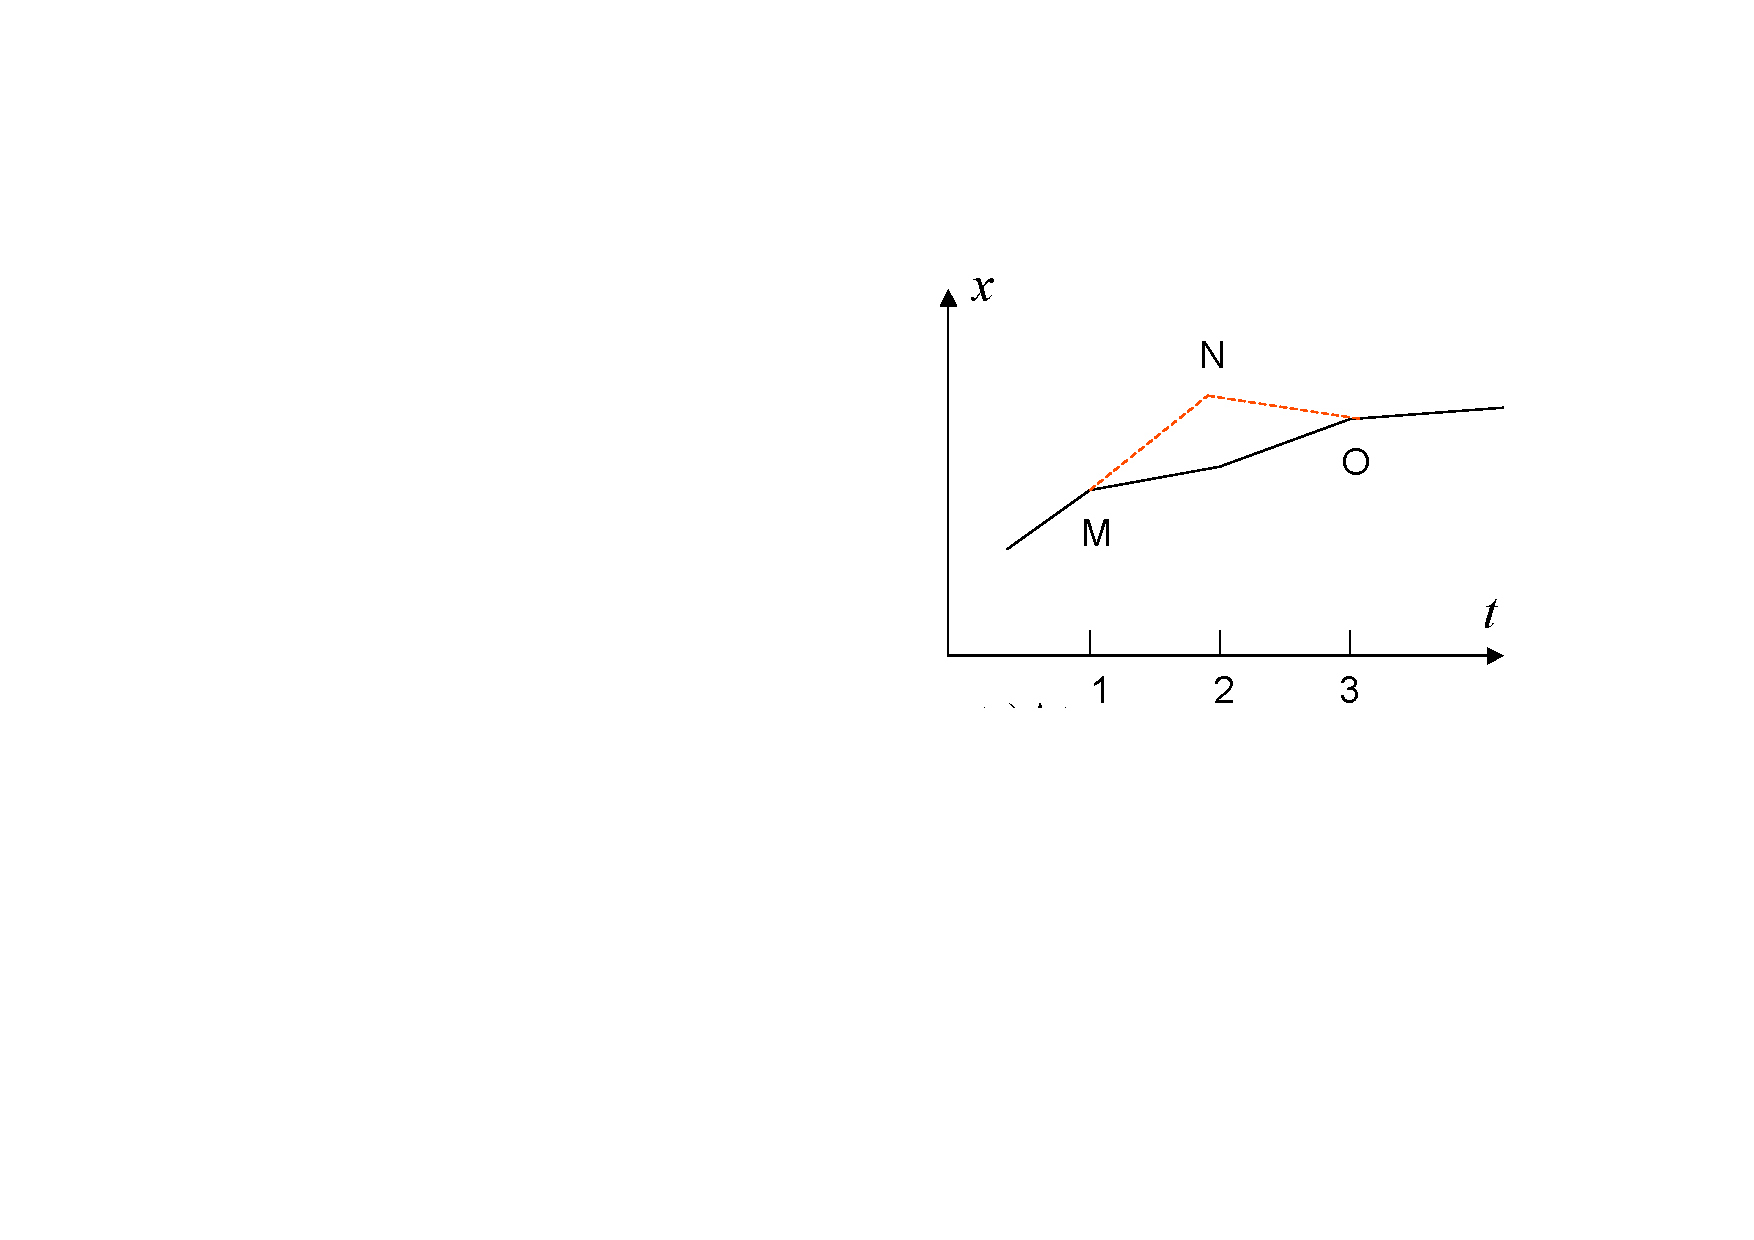
\includegraphics[width=0.5\textwidth]{./graphs/action-path.pdf}
\end{figure}
%%%
%

% position of a point
\newcommand{\pospoint}[1]{\comp{\pvec}{\point{#1}}}
% average velocity of a point
\newcommand{\avelpoint}[1]{\comp{\bar{\pvec}}{\point{#1}}}

The key observation, due to Euler, is that every section of the action integral, or sum in this case, must be stationary; \ie, it must take either a maximum or a minimum value. To see this, refer to \cref{fig:approxpath}. To find this stationary value, refer again to the figure. It shows a linearized path with the points $\point M$ and $\point O$ on it. The point between them, $\point N$ at time $t_2$, was shifted from the linearized path (approximation of the real path taken by a particle) to a higher position. Note in the figure that the positions of $\point M$, $\pospoint M$, and of $\point O$, $\pospoint O$, are fixed. 

Next, calculate the value of the action between the three points, $\action_{\point M\point N\point O}$, as the sum of the actions of the component line segments, remembering that each $\comp xi$ is taken at the beginning of each segment
\beq
\action_{\point M\point N\point O} = \lag\vat{\pospoint M, \avelpoint M, t_1}\diff t 
                                   + \lag\vat{\pospoint N, \avelpoint N, t_2}\diff t\,.
\eeq

Without loss of generality, take equal time steps: $\diff t = t_2 - t_1 = t_3 - t_2$. Then, $\avelpoint M = (\pospoint N - \pospoint M)/\diff t$ and $\avelpoint N = (\pospoint O - \pospoint N)/\diff t$.

Require then the action to be stationary noting that $\action$ is a function of $\pospoint N$ only, since the positions $\pospoint M$ and $\pospoint O$ are fixed, and using the chain rule for derivatives:
\beq
\xod{\action_{\point M\point N\point O}}{\pospoint N} 
    = \left( 
      \xpd{\lag}{\avelpoint M}\xod{\avelpoint M}{\pospoint N} 
      + \xpd{\lag}{\pospoint N}
      + \xpd{\lag}{\avelpoint N}\xod{\avelpoint N}{\pospoint N} 
      \right) \diff t = 0\,.
\eeq

Note that $\dx\avelpoint M/\dx\pospoint N = 1/\diff t$ and $\dx\avelpoint N/\dx\pospoint N = -1/\diff t$ to have
\beq
\xod{\action_{\point M\point N\point O}}{\pospoint N} 
    = \left( 
      \xpd{\lag}{\avelpoint M}\dfrac{1}{\diff t}
      + \xpd{\lag}{\pospoint N}
      - \xpd{\lag}{\avelpoint N}\dfrac{1}{\diff t} 
      \right) \diff t 
    = \xpd{\lag}{\pospoint N}
      - \dfrac{1}{\diff t}
      \left( 
      \xpd{\lag}{\avelpoint N}
      -\xpd{\lag}{\avelpoint M}
      \right)
    = 0\,.
\eeq

This last condition must hold for any point on the path, so taking $\diff t\to 0$, one has
\begin{equation}\label{eq:eleqngeometry}
\eleqn x{} = 0\,.
\end{equation}
This is to say that the condition that the action be stationary for every point of a particle trajectory implies that the particle's position $\pvec$ and velocity $\dt\pvec$ must satisfy \cref{eq:eleqngeometry}. This equation is called the Euler-Lagrange equation of motion and is the backbone of the Lagrangian description of motion, as opposed to the Newtonian description of motion.


\subsection{Classical test particle with Newtonian gravity}
Suppose we are given a particle with mass $m$ and position $\pvec\vat t$ in a Newtonian gravitation field with potential $\zeta$, where $\dim\zeta = \phdim{FL/M} = \phdim{E/M}$. The particle's world line is parameterized by time $t$. The particle's kinetic energy is~\footnote{~In geometric algebra, if $x$ is a vector, then $x^2 = xx = x\iprod x$, since $x$ is parallel to itself, and thus $x\oprod x = 0$.}
\beq
\ken\vat t = \dfrac{1}{2}m\dt\pvec^2\vat t
\eeq
and the particle's gravitational potential energy is
\beq
\pen\vat t = m\zeta\vat{\pvec\vat t, t}\,.
\eeq

Then the particle's Lagrangian is
\beq
\lag\vat t = \ken\vat t - \pen\vat t
           = \dfrac{1}{2}m\dt\pvec^2\vat t - m\zeta\vat{\pvec\vat t, t}\,.
\eeq

Varying $\pvec$ in the integral (equivalent to the Euler-Lagrange differential equation), we get
\beq
0 = \delta\int\lag\vat t\,\dx t 
  = \int\delta\lag\vat t\,\dx t
  = \int\left( m\dt\pvec\vat t\iprod \delta\dt\pvec\vat t
               - m\zeta\vat{\pvec\vat t, t}\iprod\delta\pvec\vat t
         \right)\,\dx t\,.
\eeq

Integrate the first term by parts and discard the total integral. Then divide out the variation to get
\beq
0 = -m\ddt\pvec\vat t - m\gder\zeta\vat{\pvec\vat t, t}
\eeq
and thus
\beq
m\ddt\pvec\vat t = - m\gder\zeta\vat{\pvec\vat t, t}
\eeq
is the equation of motion -- two different expressions for the force.


\subsection{Lagrangian in Vector Notation}
Using Lagrange's mechanics and vector calculus, find the equations of motion for a free particle of mass $m$.

\begin{solution}
The particle kinetic energy is $2\ken\vattpvec = m\dt\pvec^2\vat t$. Then, the particle Lagrangian becomes
\beq
\lag\vattpvec = \dfrac{1}{2}m\dt\pvec^2\vat t\,.
\eeq

Using the particle Langrangian, find the generalized force, generalized momentum and the generalized momentum time derivative
\beq
\xpd{\lag}{\pvec} = 0\,,\qquad
\xpd{\lag}{\dt\pvec} = m\dt\pvec\vat t\qquad\text{and}\qquad
\xod{}{t}\xpd{\lag}{\dt\pvec} = m\ddt\pvec\vat t\,.
\eeq

Euler-Lagrange's equations give finally the particle equations of motion:
\beq
\eleqn{\pvec}{} = m\ddt\pvec\vat t = 0\implies 
\ddt\pvec\vat t = 0\,.\mqed
\eeq
\end{solution}


Consider the last exercise particle to be object of a potential $\pen\vattpvec$. Find the particle equations of motion.

\begin{solution}
The particle Lagrangian becomes
\beq
\lag\vattpvec = \dfrac{1}{2}m\dt\pvec^2\vat t - \pen\vattpvec\,.
\eeq

Then, the generalized force, momentum and its time derivative are
\beq
\xpd{\lag}{\pvec} = -\xpd{\pen\vattpvec}{\pvec} = -\gder\pen\vattpvec \,,\qquad
\xpd{\lag}{\dt\pvec} = m\dt\pvec\vat t\qquad\text{and}\qquad
\xod{}{t}\xpd{\lag}{\dt\pvec} = m\ddt\pvec\vat t\,.
\eeq

Euler-Lagrange's equations give finally the particle equations of motion:
\beq
\eleqn{\pvec}{} = m\ddt\pvec\vat t + \gder\pen\vattpvec = 0\implies 
\ddt\pvec\vat t = -\gder\pen\vattpvec \,.\mqed
\eeq
\end{solution}




\section{Hamiltonian}
The \lingo{Hamiltonian}, $\ham$, is defined by
\beq
\ham = \igmom{}\iprod\igvel{} - \lag\,.
\eeq

The equations of motion can be found by
\beq
\igfor{i}     = -\ipd{\igpos{i}}{\ham}\,,\quad
\igvel{i}     = \ipd{\igmom{i}}{\ham}\quad\text{and}\quad
\ipd{t}{\lag} = -\ipd{t}{\ham}\,. 
\eeq

\begin{example}
Find the equation of motion for a simple pendulum. Use the Hamilton formalism of mechanics.
\end{example}

\begin{solution}
A simple pendulum is a pendulum swinging through an inviscid fluid and consisting of a bob of mass $\mass$ hanging of a inflexible, massless, frictionless rod of length $\length$. To find the equation of motion, follow pendulum amplitude $\igpos\theta$.

For the pendulum, calculate the Langrangian:
\beq
\lag = \dfrac{1}{2}\mass\length^2\left(\igvel{\theta}{}\right)^2 + \mass\grav\length\cos\vat\theta\,.
\eeq
Next, find the generalized momentum as
\beq
\igmom{\theta} = \ipd{\igvel{\theta}{}}{\lag} = \mass\grav\length\cos\vat\theta\,.
\eeq
Then, isolate the generalized velocity:
\beq
\igvel{\theta}{} = \dfrac{\igmom{\theta}}{\mass\length^2}\,.
\eeq

Replace the generalized momentum and velocity in the definition of $\ham$ to have
\beq
\ham = \igmom{\theta}\igvel{\theta}{} 
       - \dfrac{1}{2}\mass\length^2\left(\igvel{\theta}{}\right)^2 
       - \mass\length\cos\vat\theta\,,
\eeq
but $\igvel{\theta}{} = \igmom{\theta}/\mass\length^2$, thus
\beq
\ham = \dfrac{\igmom{\theta}^2}{2\mass\length^2} - \mass\grav\length\cos\vat\theta\,.
\eeq
Then, the equations of motion are
\beq
\igfor{\theta}   = -\ipd{\theta}\ham = -\mass\length\sin\vat\theta\quad\text{and}\quad
\igvel{\theta}{} = \ipd{\igmom{\theta}}{\ham} = \dfrac{\igmom{\theta}}{\mass\length^2}\,.
\eeq
Finally, taking the derivative of the generalized velocity and replacing into the generalized momentum, one has the equation of motion for the simple pendulum
\beq
\igacc{\theta}{} = -\dfrac{\grav}{\length}\sin\vat\theta\,.\mqed
\eeq
\end{solution}



\section{Classical Dynamics}

[Classical Dynamics, Dr David Tong, 2004-2005]

\subsection{Newtonian Mechanics: A Single Particle}
Basic concepts: a particle is defined to be an object of insignificant size; \eg, an electron, a tennis ball or a planet. Obviously the validity of this statement depends on the context: to first approximation, the earth can be treated as a particle when computing its orbit around the sun. But if you want to understand its spin, it must be treated as an extended object.

The motion of a particle of mass $m$ at the position $\pvec$ is governed by Newton's Second Law $f=ma$ or, more precisely,
\beq
f\vat{\pvec,\dt\pvec} = \dt\lmom\,,
\eeq
where $f$ is the force which, in general, can depend on both the position $\pvec$ as well as the velocity $\dt\pvec$, (for example, friction forces depend on $\dt\pvec$) and $\lmom = m\dt\pvec$ is the momentum. Both $f$ and $\lmom$ are 3-vectors. The last equation reduces to $f = ma$ if $\dt m = 0$. But if $m = m\vat t$ (\eg, in rocket science), then the form with $\dt\lmom$ is correct.

General theorems governing differential equations guarantee that if we are given $\pvec$ and $\dt\pvec$ at an initial time $t = t_0$, we can integrate the last equation to determine $\pvec\vat t$ for all $t$ (as long as $f$ remains finite). This is the \emph{goal of classical dynamics}.

The last is not quite correct as stated: we must add the caveat that it holds \emph{only} in an \lingo{inertial frame}. This is defined to be a frame in which a free particle with $\dt m = 0$ travels in a straight line,
\beq
\pvec = \pvec_0 + \dt\pvec t\,,
\eeq
Newton's first law is the statement that such frames exist.

Angular momentum: we define the angular momentum $l$ of a particle and the torque $\tau$ acting upon it as
\beq
l = \pvec\cprod\lmom\qquad\text{and}\qquad\tau = \pvec\cprod f\,.
\eeq
Note that, unlike linear momentum $\lmom$, both $l$ and $\tau$ depend on where we take the origin: \emph{we measure angular momentum with respect to a particular point}. Let us cross both sides of the last equation with $\pvec$. Using the fact that $\dt\pvec$ is parallel to $\lmom$, we can write
\beq
\xod{(\pvec\cprod\lmom)}{t} = \pvec\cprod\dt\lmom\,.
\eeq
Then we get a version of Newton's second law that holds for angular momentum:
\beq
\tau = \dt l\,.
\eeq

Conservation Laws: From the last equations, two important conservation laws follow immediately. 
\begin{itemize}
\item If $f = 0$, then $\lmom$ is constant throughout the motion;
\item If $\tau = 0$, then $l$ is constant throughout the motion.
\end{itemize}
Notice that $\tau = 0$ does not require $f = 0$, but only $\pvec\cprod f = 0$. This means that $f$ \emph{must} be parallel to $\pvec$. This is the definition of a \lingo{central force}. An example is given by the gravitational force between the earth and the sun: the earth's angular momentum about the sun is constant. As written above in terms of forces and torques, these conservation laws appear trivial.

Energy: Let's now recall the definitions of energy. We firstly define the kinetic energy $\ken$ as
\beq
\ken = \dfrac{1}{2}m\dt\pvec\iprod\dt\pvec\,.
\eeq
Suppose from now on that the mass is constant. We can compute the change of kinetic energy with time: $\dt\ken = \dt\lmom\iprod\dt\pvec = f\iprod\dt\pvec$. If the particle travels from position $\pvec_1$ at time $t_1$ to position $\pvec_2$ at time $t_2$ then this change in kinetic energy is given by
\beq
\ken\vat{t_2} - \ken\vat{t_1} = \int_{t_1}^{t_2}\dt\ken\,\dx t
                              = \int_{t_1}^{t_2}f\iprod\dt\pvec\,\dx t
                              = \int_{\pvec_1}^{\pvec_2}f\iprod\dx\pvec\,,
\eeq
where the final expression involving the integral of the force over the path is called the \lingo{work done by the force}. So we see that 
\begin{quote}
the work done is equal to the change in kinetic energy. 
\end{quote}
From now on we will mostly focus on a very special type of force known as a \lingo{conservative force}. Such a force depends only on position $\pvec$ rather than velocity $\dt\pvec$ and is such that the work done is \emph{independent of the path taken}. In particular, for a closed path, the work done vanishes:
\beq
\oint f\iprod\dx\pvec \iff \gder\cprod f = 0\,.
\eeq

It is a deep property of flat space $\espace 3$ that this property implies we may write the force as
\beq
f = -\gder\pen\vat\pvec
\eeq
for some potential $\pen\vat\pvec$. Systems which admit a potential of this form include gravitational, electrostatic and interatomic forces. When we have a conservative force, we necessarily have a conservation law for energy. To see this, return to the change of kinetic energy equation which now reads
\beq
\ken\vat{t_2} - \ken\vat{t_1} = \int_{\pvec_1}^{\pvec_2}f\iprod\dx\pvec
                              = -\int_{\pvec_1}^{\pvec_2}\gder\pen\iprod\dx\pvec
                              = -\pen\vat{t_2} + \pen\vat{t_1}\,,
\eeq
or, rearranging things,
\beq
\ken\vat{t_1} + \pen\vat{t_1} = \ken\vat{t_2} + \pen\vat{t_2} = e\,.
\eeq
So $e = \ken + \pen$ is also a \lingo{constant of motion}. It is the energy. When the energy is considered to be a function of position $\pvec$ and momentum $\lmom$ it is referred to as the \lingo{Hamiltonian} $\ham$.

Example 1: The Simple Harmonic Oscillator. This is a one-dimensional system with a force proportional to the distance $\pvec$ to the origin: $f\vat x = -k\pvec$. This force arises from a potential $2\pen = k\pvec^2$. Since $f\neq 0$,  momentum is \emph{not} conserved (the object oscillates backwards and forwards) and, since the system lives in only one dimension, angular momentum is \emph{not defined}. But energy
\beq
e = \dfrac{1}{2}m\dt\pvec^2 + \dfrac{1}{2}k\pvec^2
\eeq
is conserved.

Example 2: The Damped Simple Harmonic Oscillator. We now include a friction term so that $f\vat{\pvec,\dt\pvec} = -k\pvec - \gamma\dt\pvec$. Since $f$ is not conservative, energy is \emph{not} conserved. This system loses energy until it comes to rest. (The last statement is not entirely true. Mechanical energy is not conserved, but total energy is, because mechanical energy transforms into heating and then the system comes to rest.)

Example 3: Particle Moving Under Gravity. Consider a particle of mass $m$ moving in three dimensions under the gravitational pull of a much larger particle of mass $M$. The force is $f = -(GmM/\pvec^2)\nvec\pvec$ which arises from the potential $\pen = -GmM/\pvec$. Again, the linear momentum $\lmom$ of the smaller particle is \emph{not} conserved, but the force is both central and conservative, ensuring the particle's total energy $e$ and the angular momentum $l$ are conserved.


\subsection{The Principle of Least Action - The Lagrangian Formalism}
Firstly, let's get our notation right. Part of the power of the Lagrangian formulation over the Newtonian approach is that 
\begin{quote}
the Lagrangian formulation does away with vectors in favor of more general coordinates. 
\end{quote}
We start by doing this trivially. Let's rewrite the positions of $N$ particles with coordinates $\pvec_i$ as $\gpos i$ where $i=1,\dotsc,3N$. Then Newton's equations read
\begin{equation}\label{eq:newtonslawofmotion}
\dt{\gmom i} = -\xpd{\pen}{\gpos i}\,,
\end{equation}
where $\gmom i = m_i\gvel i$. The number of degrees of freedom of the system is said to be $3$N. These parameterize a $3N$-dimensional space known as the \lingo{configuration space} $C$. Each point in $C$ specifies a configuration of the system (\ie, the positions of all $N$ particles). Time evolution gives rise to a curve in $C$.

Define the \lingo{Lagrangian} to be a function of the positions $\gpos i$ and the velocities $\gvel i$ of all the particles, given by~\footnote{~The Lagrangian is defined as the difference of two energies, therefore it has the dimensions of energy $\phdim E$; \ie, $\dim\lag = \phdim E$.}
\beq
\lag\vat{\gpos i,\gvel i} = \ken\vat{\gvel i} - \pen\vat{\gpos i}\,,
\eeq
where $2\ken = \sum_i m_i (\gvel i)^2$ is the kinetic energy and $\pen\vat{\gpos i}$ is the potential energy. Note the minus sign between $\ken$ and $\pen$! To describe the principle of least action, we consider all smooth paths $\gpos i\vat t$ in $C$ with fixed end points so that
\beq
\gpos i\vat{t\txt i} = \gpos i\txt{initial}\qquad\text{and}\qquad\gpos i\vat{t\txt f} = \gpos i\txt{final}\,.
\eeq
Of all these possible paths, only one is the true path taken by the system. Which one? To each path, let us assign a number called the action $\action$ defined as
\beq
\action\vat{\gpos i\vat t} = \int_{t\txt{initial}}^{t\txt{final}}\lag\vat{\gpos i,\gvel i}\,\dx t\,.
\eeq
The action is a \lingo{functional} (\ie, a function of the path which is itself a function). The principle of least action is the following result:

Theorem (Principle of Least Action): The actual path taken by the system is an \lingo{extremum} of $\action$.

[proof: omitted]

This requirement holds if and only if
\begin{equation}\label{eq:eulerlagrangeequations}
\eleqn{\gpvec}{i} = 0\qquad\text{for each $i=1,\dotsc,3N$}\,.
\end{equation}
These are known as \lingo{Lagrange's equations} (or sometimes as the \lingo{Euler-Lagrange equations}). 

Lagrange's equations are equivalent to Newton's. From the definition of the Lagrangian, we have $\partial\lag/\partial\gpos i = -\partial\pen/\gpos i$, while $\partial\lag/\partial\gvel i = \gmom i$. It's then easy to see that \cref{eq:eulerlagrangeequations} are indeed equivalent to \cref{eq:newtonslawofmotion}.

\begin{note}
The $\gpos i$ are called \lingo{generalized coordinates}, while the $\gvel i$ are called \lingo{generalized velocities}. Both have \lingo{contravariant} components:
\begin{align*}
\dim \gpos i = \phdim{L}   &\implies\text{contravariant components}\,,\\
\dim \gvel i = \phdim{L/T} &\implies\text{contravariant components}\,.
\end{align*}

The first terms in \cref{eq:eulerlagrangeequations} are called \lingo{generalized forces}, $\gfor i$,
\beq
\gfor i = \xpd{\lag}{\gpos i}\,,
\eeq
while the second terms are called \lingo{generalized momenta}, $\gmom i$,
\beq
\gmom i = \xpd{\lag}{\gvel i}\,.
\eeq
Thus, Euler-Lagrange equations, \cref{eq:eulerlagrangeequations}, can be written in a form analogous to Newton's second law of motion:
\beq
\gfor i = \dt{\gmom i}\,,
\eeq
this is, generalized forces equal the time change of generalized momenta.

Additionally, notice that both generalized forces and momenta have \lingo{covariant components}:
\begin{align*}
\dim \gfor i = \xpd{\lag}{\gpos i} = \phdim{E/L}             &\implies\text{covariant components}\,,\\
\dim \gmom i = \xpd{\lag}{\gvel i} = \phdim{E.T/L} &\implies\text{covariant components}\,,
\end{align*}
where $\phdim{E}$ stands for the dimension of energy.

Finally, note that generalized momenta are the \lingo{conjugate} of generalized coordinates:
\beq
\gmom i = \xpd{\lag}{\gvel i}\,.
\eeq
\end{note}

Some remarks on this important result:
\begin{itemize}
\item This is an example of a variational principle.
%
\item The principle of least action is a slight misnomer. The proof only requires that $\delta\action = 0$ and does not specify whether it is a maxima or minima of $\action$. Since $\lag = \ken - \pen$, we can always increase $\action$ by taking a very fast, wiggly path with $\ken\gg 0$, so the true path is never a maximum. However, it may be either a minimum or a saddle point. So \lingo{Principle of stationary action} would be a more accurate, but less catchy, name. It is sometimes called \lingo{Hamilton's principle}.
%
\item All the fundamental laws of physics can be written in terms of an action principle. This includes electromagnetism, general relativity, the standard model of particle physics and attempts to go beyond the known laws of physics such as string theory.
%
\item There is a beautiful generalization of the action principle to quantum mechanics due to Feynman in which the particle takes all paths with some probability determined by $\action$.
%
\item Back to classical mechanics, there are two very important reasons for working with Lagrange's equations rather than with Newton's. The first is that Lagrange's equations hold in any coordinate system, while Newton's are restricted to an inertial frame. The second is the ease with which we can deal with constraints in the Lagrangian system.
\end{itemize}


\subsection{Changing Coordinate Systems}
Lagrange's equations hold in \emph{any} coordinate system. This follows immediately from the action principle, which is a statement about paths and not about coordinates. So the \lingo{form} of Lagrange's equations holds in any coordinate system. This is in contrast to Newton's equations which are only valid in an inertial frame. Let's illustrate the power of this fact with an example.

Example: Rotating Coordinate Systems: Consider a free particle with Lagrangian given by
\beq
\lag = \dfrac{1}{2}m\dt\pvec^2\,,
\eeq
with $\pvec = \tuple{x,y,z}$. Now measure the motion of the particle with respect to a coordinate system which is rotating with angular velocity $\omega = \tuple{0,0,\omega}$ about the $z$ axis. If $\pvec' = \tuple{x',y',z'}$ are the coordinates in the rotating system, we have the relationship
\begin{align*}
x' &= x\cos\vat{\omega t} + y\sin\vat{\omega t}\,,\\
y' &= y\cos\vat{\omega t} - x\sin\vat{\omega t}\,,\\
z' &= z\,.
\end{align*}

Then we can substitute these expressions into the Lagrangian to find $\lag$ in terms of the rotating coordinates,
\beq
\lag = \dfrac{1}{2}m \left( (\dt x' - \omega y')^2 + (\dt y' + \omega x')^2 + \dt z^2 \right)
     = \dfrac{1}{2}m(\dt\pvec' + \omega\cprod\pvec')^2\,.
\eeq
In this rotating frame, we can use Lagrange's equations to derive the equations of motion. Taking derivatives, we have
\begin{align*}
\xpd{\lag}{\pvec'}             &= m\left(\dt\pvec'\cprod\omega - \omega\cprod(\omega\cprod\pvec') \right) \,,\\
\xod{}{t}\xpd{\lag}{\dt\pvec'} &= m\left(\ddt\pvec' + \omega\cprod\dt\pvec' \right)\,,
\end{align*}
so Lagrange's equation reads
\beq
\xod{}{t}\xpd{\lag}{\dt\pvec'} - \xpd{\lag}{\pvec'} 
    = m\left(\ddt\pvec' 
      + \omega\cprod(\omega\cprod\pvec') 
      + 2\omega\cprod\dt\pvec'\right) = 0\,.
\eeq
The second and third terms in this expression are the \lingo{centrifugal} and \lingo{coriolis forces}. These are examples of the \lingo{fictitious forces}. They're called fictitious because they're a consequence of the reference frame, rather than any interaction. But don't underestimate their importance just because they're ``fictitious''! According to Einstein's theory of general relativity, the force of gravity is on the same footing as these fictitious forces.


\subsection{Constraints and Generalized Coordinates}
Define the operator $\igder i = \partial/\partial\gpos i$.

Now we turn to the second advantage of the Lagrangian formulation. In writing $\gfor i = \dt{\gmom i} = -\igder i\pen$, we implicitly assume that each particle can happily roam anywhere in space $\espace 3$. What if there are constraints? In Newtonian mechanics, we introduce \lingo{constraint forces}. These are things like the tension of ropes and normal forces applied by surfaces. In the Lagrangian formulation, we don't have to worry about such things. 

An Example: The Pendulum. The simple pendulum has a single dynamical degree of freedom $\theta$, the angle the pendulum makes with the vertical. The position of the mass $m$ in the plane is described by two Cartesian coordinates $x$ and $y$ subject to a constraint $x^2 + y^2 = l^2$. We can parameterize this as $x = l\sin\vat\theta$ and $y = l\cos\vat\theta$. Employing the Newtonian method to solve this system, we introduce the tension $T$ and resolve the force vectors to find
\beq
m\ddt x = -Tx/l\qquad\text{and}\qquad m\ddt y = mg - Ty/l\,.
\eeq
To determine the motion of the system, we impose the constraints at the level of the equation of motion, and then easily find
\beq
\ddt\theta = -(g/l)\sin\vat\theta\qquad\text{and}\qquad T = ml\dt\theta^2 + mg\cos\vat\theta\,.
\eeq

While this example was pretty straightforward to solve using Newtonian methods, things get rapidly harder when we consider more complicated constraints (and we'll see plenty presently). Moreover, you may have noticed that half of the work of the calculation went into computing the tension $T$. On occasion we'll be interested in this. (For example, we might want to know how fast we can spin the pendulum before it breaks). But often we won't care about these constraint forces, but will only want to know the motion of the pendulum itself. In this case it seems like a waste of effort to go through the motions of computing $T$. We'll now see how we can avoid this extra work in the Lagrangian formulation. Firstly, let's define what we mean by constraints more rigorously.

\subsubsection{Holonomic Constraints} \lingo{Holonomic Constraints}~\footnote{~Introduced by H. Hertz in 1894, the term \lingo{holonomic} comes from the Greek and means whole law.} are relationships between the coordinates of the form
\beq
\gfor\alpha\vat{\pvec^i, t} = 0\qquad\alpha = 1,\dotsc, 3N-n\,.
\eeq
In general the constraints can be time dependent and our notation above allows for this. Holonomic constraints can be solved in terms of $n$ \lingo{generalised coordinates} $\setprop{\gpos i}{i = 1,\dotsc,n}$. So 
\beq
\pvec^i = \pvec^i\vat{\gpos 1, \dotsc, \gpos n}\,.
\eeq
The system is said to have $n$ degrees of freedom. For the pendulum example above, the system has a single degree of freedom, $\gpos 1 = \gpos{} = \theta$. 

One method to use the Lagrangian formulation is to introduce constraints of this form: introduce $3N-n$ new variables $\lambda_\alpha$, called \lingo{Lagrange multipliers} and define a new Lagrangian. So we can incorporate constraint forces into the Lagrangian setup using Lagrange multipliers. But the big news is that we don't have to! Often we don't care about constraint forces, but only want to know what the generalized coordinates $\gpos i$ are doing. In this case we have the following useful theorem:

Theorem: For constrained systems, we may derive the equations of motion directly in generalized coordinates $\gpos i$
\beq
\lag\vat{\gpos i, \gvel i, t} = \lag\vat{\pvec^i\vat{\gpos i,t}, \dt\pvec^i\vat{\gpos i,t}} \,.
\eeq

If we are only interested in the dynamics of the generalized coordinates $\gpos i$, we may ignore the Lagrange multipliers and work entirely with the unconstrained Lagrangian $\lag\vat{\gpos i, \gvel i, t}$ defined in the last equation where we just substitute in $\pvec^i = \pvec^i\vat{\gpos i,t}$.

Let's see how this works in the simple example of the pendulum. We can parameterize the constraints in terms of the generalized coordinate $\theta$ so that $x = l\sin\vat\theta$ and $y = l\cos\vat\theta$. We now substitute this directly into the Lagrangian for a particle moving in the plane under the effect of gravity, to get
\beq
\lag = \dfrac{1}{2}m\left(\dt x^2 + \dt y^2\right) + mgy = \dfrac{1}{2}ml^2\dt\theta^2 + mgl\cos\vat\theta\,.
\eeq
From which we may derive Lagrange's equations using the coordinate $\theta$ directly
\beq
\eleqn{\theta}{} = ml^2\ddt\theta + mgl\sin\vat\theta = 0\,,
\eeq
which indeed reproduces the equation of motion for the pendulum; \viz, $\ddt\theta = -(g/l)\sin\vat\theta$. Note that, as promised, we haven't calculated the tension $T$ using this method. This has the advantage that we've needed to do less work. If we need to figure out the tension, we have to go back to the more laborious Lagrange multiplier or Newton methods.

\subsubsection{Non-Holonomic Constraints} 
For completeness, let's quickly review a couple of non-holonomic constraints. There's no general theory to solve systems of this type, although it turns out that both of the examples we describe here can be solved with relative ease using different methods.

Inequalities: Consider a particle moving under gravity on the outside of a sphere of radius $r$. It is constrained to satisfy $z^2 + y^2 + z^2 \geq r^2$. This type of constraint, involving an inequality, is non-holonomic. When the particle lies close to the top of the sphere, we know that it will remain in contact with the surface and we can treat the constraint effectively as holonomic. But at some point the particle will fall off. To determine when this happens requires different methods from those above (although it is not particularly difficult).

Velocity Dependent Constraints: Constraints of the form $g\vat{\pvec^i, \dt{\pvec^i}, t} = 0$ which cannot be integrated to give $f\vat{\pvec^2,t} = 0$ are non-holonomic. For example, consider a coin of radius $r$ rolling down a slope. The coordinates $\tuple{x,y}$ fix the coin's position on the slope. But the coin has other degrees of freedom as well: the angle $\theta$ it makes with the path of steepest descent, and the angle $\phi$ that a marked point on the rim of the coin makes with the vertical. If the coin rolls without slipping, then there are constraints on the evolution of these coordinates. We must have that the velocity of the rim is $v\txt{rim} = r\phi$. So, in terms of our four coordinates, we have the constraint
\beq
x = r\dt\phi\sin\vat\theta\qquad\text{and}\qquad y = r\dt\phi\cos\vat\theta\,. 
\eeq
But these cannot be integrated to give constraints of the form $f\vat{x,y,\theta,\phi} = 0$. They are non-holonomic.

\subsection{Summary}
Let's review what we've learnt so far. A system is described by $n$ generalized coordinates $\gpos i$ which define a point in an $n$-dimensional configuration space $C$. Time evolution is a curve in $C$ governed by the Lagrangian 
\beq
\lag\vat{\gpos i,\gvel i, t}
\eeq
such that the $\gpos i$ obey
\beq
\eleqn{\gpvec}{i} = 0\,.
\eeq
These are $n$ coupled 2nd order (usually) non-linear differential equations. 

Before we move on, let's take this opportunity to give an important definition. The quantity
\beq
\gmom i = \xpd{\lag}{\gvel i}
\eeq
is called the \lingo{generalised momentum conjugate to $\gpos i$}. (It only coincides with the real momentum in Cartesian coordinates). We can now rewrite Lagrange's equations as
\beq
\dt{\gmom i} = \xpd{\lag}{\gpos i}\,.
\eeq


\subsection{Noether's Theorem and Symmetries}
In this subsection we shall discuss the appearance of conservation laws in the Lagrangian formulation and, in particular, a beautiful and important theorem due to Noether relating conserved quantities to symmetries.

Let's start with a definition. A function $f\vat{\gpos i, \gvel i, t}$ of the coordinates, their time derivatives and (possibly) time $t$ is called a \lingo{constant of motion} (or a \lingo{conserved quantity}) if the total time derivative vanishes (an application of the chain rule!)
\beq
\xod{f}{t} = \sum_{j = 1}^{n}\left( \xpd{f}{\gpos j}\gvel j + \xpd{f}{\gvel j}\gacc j \right) + \xpd{f}{t}\,,
\eeq
whenever $\gpos i\vat t$ satisfy Lagrange's equations. This means that $f$ remains constant along the path followed by the system. Here's a couple of examples:

Claim: If $\lag$ does not depend explicitly on time $t$ (\ie, $\partial\lag/\partial t = 0$), then
\beq
\ham = \sum_j \gvel j\xpd{\lag}{\gvel j} - \lag
\eeq
is constant. When $\ham$ is written as a function of $\gpos i$ and $\gmom i$, it is known as the \lingo{Hamiltonian}. It is usually identified with the total energy of the system.

Claim: Suppose $\partial\lag/\partial\gpos j = 0$ for some $\gpos j$. Then, $\gpos j$ is said to be \lingo{ignorable} (or \lingo{cyclic}). We have the conserved quantity
\beq
\gmom j = \xpd{\lag}{\gvel j}\,.
\eeq

\subsubsection{Noether's Theorem}
Consider a one-parameter family of maps
\beq
\gpos i\vat t\to\cnvec Qi\vat{s,t}\qquad\text{with}\qquad s\in\set R
\eeq
such that $\cnvec Qi\vat{0,t} = \gpos i\vat t$. Then, this transformation is said to be a \lingo{continuous symmetry of the Lagrangian} $\lag$ if
\beq
\xpd{}{s}\lag\vat{\cnvec Qi\vat{s,t}, \dt{\cnvec Qi}\vat{s,t}, t} = 0\,.
\eeq
Noether's theorem states that 
\begin{quote}
for each such symmetry there exists a conserved quantity.
\end{quote}

Homogeneity of Space: 
\begin{quote}
Homogeneity of Space implies Translation Invariance of $\lag$ implies Conservation of Total Linear Momentum.
\end{quote}
This statement should be intuitively clear. One point in space is much the same as any other. So why would a system of particles speed up to get over there, when here is just as good? This manifests itself as conservation of linear momentum.

Isotropy of Space:
\begin{quote}
Isotropy of Space implies Rotational Invariance of $\lag$ implies Conservation of Total Angular Momentum.
\end{quote}

Homogeneity of Time: What about homogeneity of time? In mathematical language, this means $\lag$ is invariant under $t\to t + s$ or, in other words, $\partial\lag/\partial t = 0$. But we already saw earlier in this section that this implies 
\beq
\ham = \sum_i \gvel i\left( \xpd{\lag}{\gvel i} \right) - \lag 
\eeq
is conserved. In the systems we’re considering, this is simply the total energy. We see that the existence of a conserved quantity which we call energy can be traced to the homogeneous passage of time. Or
\begin{quote}
Time is to Energy as Space is to Momentum.
\end{quote}
Recall from your course on special relativity that energy and 3-momentum fit together to form a 4-vector which rotates under spacetime transformations. Here we see that the link between energy-momentum and time-space exists even in the non-relativistic framework of Newtonian physics. You don't have to be Einstein to see it. You just have to be Emmy Noether.

\begin{note}
It turns out that \emph{all} conservation laws in nature are related to symmetries through Noether's theorem. This includes the conservation of electric charge and the conservation of particles such as protons and neutrons (known as baryons).
\end{note}


\subsection{Applications}

\subsubsection{Bead on a Rotating Hoop}
This is an example of a system with a time dependent holonomic constraint. The hoop is of radius a and rotates with frequency $\omega$. The bead, of mass $m$, is threaded on the hoop and moves without friction. We want to determine its motion. There is a single degree of freedom $\phi$, the angle the bead makes with the vertical. In terms of Cartesian coordinates $\tuple{x,y,z}$ the position of the bead is
\beq
x = a\sin\vat\phi\cos\vat{\omega t}\,,\quad y = a\sin\vat\phi\sin\vat{\omega t}\quad\text{and}\quad z = a - a\cos\vat\phi\,.
\eeq
To determine the Lagrangian in terms of the generalized coordinate $\phi$ we must substitute these expressions into the Lagrangian for the free particle. For the kinetic energy $\ken$ we have
\beq
\ken = \dfrac{1}{2}m\left(x^2 + y^2 + z^2\right) = \dfrac{1}{2}ma\left(\dt\phi^2 + \omega^2\sin^2\vat{\phi}\right)\,,
\eeq
while the potential energy $\pen$ is given by (ignoring an overall constant)
\beq
\pen = mgz = -mga\cos\vat\phi\,.
\eeq
So, replacing $x$, $y$ and $z$ by $\phi$, we have the Lagrangian
\beq
\lag = ma^2\left(\dfrac{1}{2}\dt\phi^2 - \pen\txt{eff}\right)
\eeq
where the effective potential is
\beq
\pen\txt{eff} = \dfrac{1}{ma^2}\left(-mga\cos\vat\phi - \dfrac{1}{2} ma^2\omega^2\sin^2\vat\phi\right)\,.
\eeq

We can now derive the equations of motion for the bead simply from Lagrange's equations which read
\beq
\ddt\phi = -\xpd{\pen\txt{eff}}{\phi}\,.
\eeq

Let's look for stationary solutions of these equations in which the bead doesn't move (\ie, solutions of the form $\ddt\phi = \dt\phi = 0$). From the equation of motion, we must solve $\partial\pen\txt{eff}/\partial\phi = 0$ to find that the bead can remain stationary at points satisfying
\beq
g\sin\vat\phi = a\omega^2\sin\vat\phi\cos\vat\phi\,.
\eeq

There are at most three such points: $\phi = 0$, $\phi = \pi$ or $\cos\vat\phi = g/a\omega^2$. Note that the first two solutions always exist, while the third stationary point is only there if the hoop is spinning fast enough so that $\omega^2\geq g/a$. Which of these stationary points is stable depends on whether $\pen\txt{eff}\vat\phi$ has a local minimum (stable) or maximum (unstable). This in turn depends on the value of $\omega$.


\subsubsection{Spherical Pendulum}
The spherical pendulum is allowed to rotate in three dimensions. The system has two degrees of freedom which cover the range $0\leq\theta < \pi$ and $0\leq\phi < 2\pi$. In terms of cartesian coordinates, we have
\beq
x = l\cos\vat\phi\sin\vat\theta\,,\quad y = l\sin\vat\phi\sin\vat\theta\quad\text{and}\quad z = -l\cos\vat\theta\,.
\eeq

We substitute these constraints into the Lagrangian for a free particle to get
\beq
\lag = \dfrac{1}{2}m\left(\dt x^2 + \dt y^2 + \dt z^2\right) 
     = \dfrac{1}{2}ml^2\left(\dt\theta^2 + \dt\phi^2\sin^2\vat\theta\right) + mgl\cos\vat\theta\,.
\eeq

Notice that the coordinate $\phi$ is ignorable (it does not appear explicitly in the Lagrangian). From Noether's theorem, we know that the quantity
\beq
J = \xpd{\lag}{\dt\phi} = ml^2\dt\phi\sin^2\vat\theta\,.
\eeq
is constant. This is the component of angular momentum in the $\phi$ direction. The equation of motion for $\theta$ follows from Lagrange's equations and is
\beq
ml^2\ddt\theta = ml^2\dt\phi^2\sin\vat\theta\cos\vat\theta - mgl\sin\vat\theta\,.
\eeq

We can substitute $\dt\phi$ for the constant $J$ in this expression to get an equation entirely in terms of $\theta$ which we chose to write as
\beq
\ddt\theta = -\xpd{\pen\txt{eff}}{\theta}\,,
\eeq
where the effective potential is defined to be 
\beq
\pen\txt{eff} = -\dfrac{g}{l}\cos\vat\theta + \dfrac{J^2}{2m^2l^4}\dfrac{1}{\sin^2\vat\theta}\,.
\eeq

An important point here: we must substitute for $J$ into the equations of motion. If you substitute $J$ for $\dt\phi$ directly into the Lagrangian, you will derive an equation that looks like the one above, but you'll get a minus sign wrong! This is because Lagrange's equations are derived under the assumption that $\theta$ and $\phi$ are independent.

As well as the conservation of angular momentum $J$, we also have $\partial\lag/\partial t = 0$ so energy is conserved. This is given by
\beq
e = \dfrac{1}{2}\dt\theta^2 + \pen\txt{eff}\vat\theta\,,
\eeq
where $e$ is a constant. In fact we can invert this equation for $e$ to solve for $\theta$ in terms of an integral
\beq
t - t_0 = \dfrac{1}{\sqrt{2}}\int\dfrac{\dx\theta}{\sqrt{e - \pen\vat\theta}}\,.
\eeq

If we succeed in writing the solution to a problem in terms of an integral like this then we say we've ``reduced the problem to quadrature''. It's kind of a cute way of saying we can't do the integral. But at least we have an expression for the solution that we can play with or, if all else fails, we can simply plot on a computer.

Once we have an expression for $\theta\vat t$ we can solve for $\phi\vat t$ using the expression for $J$,
\beq
\phi = \int\dfrac{J}{ml^2}\dfrac{\dx t}{\sin^2\vat\theta} 
     = \dfrac{J}{\sqrt{2}ml^2}\int\dfrac{1}{\sqrt{e - \pen\txt{eff}}}\,\dx\theta\,,
\eeq
which gives us $\phi = \phi\vat\theta = \phi\vat t$.


\subsubsection{Purely Kinetics Lagrangians}
Often in physics, one is interested in systems with only kinetic energy and no potential energy. For a system with $n$ dynamical degrees of freedom $\gpos a$, $a = 1,\dotsc, n$, the most general form of the Lagrangian with just a kinetic term is
\begin{equation}\label{eq:mostgenerallagrangianform}
\lag = \dfrac{1}{2}\imet ab\vat{\covec qc}\gvel a\gvel b\,.
\end{equation}
The functions $\imet ab = \imet ba$ depend on all the generalized coordinates. Assume that $\det{\imet ab} \neq 0$ so that the inverse matrix $\rmet ab$ exists ($\rmet ab\imet bc = \mkron ac$). It is a short exercise to show that Lagrange's equation for this system are given by
\begin{equation}\label{eq:geodesicequationslagrangeform}
\gacc a + \Gamma^a_{bc}\gvel b\gvel c = 0\,,
\end{equation}
where
\beq
\Gamma^a_{bc} = \dfrac{1}{2}\imet ad\left( 
                \xpd{\imet bd}{\gpos c} 
                + \xpd{\imet cd}{\gpos b} 
                - \xpd{\imet bc}{\gpos d} 
                \right)\,.
\eeq
The functions $\imet ab$ define a \lingo{metric} on the configuration space and the equations \cref{eq:geodesicequationslagrangeform} are known as the \lingo{geodesic equations}. They appear naturally in general relativity where they describe a particle moving in curved spacetime. Lagrangians of the form \cref{eq:mostgenerallagrangianform} also appear in many other areas of physics, including the condensed matter physics, the theory of nuclear forces and string theory. In these contexts, the systems are referred to as \lingo{sigma models}.


\subsubsection{Particles in Electromagnetic Fields}
We saw from the beginning that the Lagrangian formulation works with conservative forces which can be written in terms of a potential. It is no good at dealing with friction forces which are often of the type $f = -k\dt\pvec$. But there are other velocity dependent forces which arise in the fundamental laws of Nature. It's a crucial fact about Nature that all of these can be written in Lagrangian form. Let's illustrate this in an important example.

Recall that the electric field $E$ and the magnetic field (magnetic induction!) $B$ can be written in terms of a vector potential $A\vat{\pvec,t}$ and a scalar potential $\phi\vat{\pvec,t}$
\beq
B = \gder\cprod A\qquad\text{and}\qquad E = -\gder\phi - \dfrac{1}{c}\xpd{A}{t}\,,
\eeq
where $c$ is the speed of light. Let's study the Lagrangian for a particle of electric charge $e$ of the form,
\beq
\lag = \dfrac{1}{2}m\dt\pvec^2 - e\left( \phi - \dfrac{1}{c}\dt\pvec\iprod A \right)\,.
\eeq

The momentum conjugate to $\pvec$ is
\beq
\lmom = \xpd{\lag}{\dt\pvec} = m\dt\pvec + \dfrac{e}{c}A\,.
\eeq
Notice that the momentum is not simply $m\dt\pvec$; it's modified in the presence of electric and magnetic fields. Now we can calculate Lagrange's equations
\beq
\xod{}{t}\xpd{\lag}{\dt\pvec} - \xpd{\lag}{\pvec} = \xod{}{t}\left( m\dt\pvec + \dfrac{e}{c}A \right)
    + e\gder\phi - \dfrac{e}{c}\gder\left(\dt\pvec\iprod A\right) = 0\,.
\eeq

To disentangle this, let's work with indices $a, b = 1, 2, 3$ on the Cartesian coordinates and rewrite the equation of motion as
\beq
m\ivec{\ddt\pvec} a = - e\left( \xpd{\phi}{\ivec\pvec a} + \dfrac{1}{c}\xpd{\covec Aa}{t} \right) 
                      + \dfrac{e}{c}\left( \xpd{\covec Ab}{\ivec\pvec a} - \xpd{\covec Aa}{\ivec\pvec b} \right)\ivec{\dt\pvec} b\,.
\eeq

Now we use our definitions of the $E$ and $B$ fields which, in terms of indices, read
\beq
\covec Ea = -\xpd{\phi}{\ivec\pvec a} - \dfrac{1}{c}\xpd{\covec Aa}{t}\qquad \covec Bc = \lct_{cab}\xpd{\covec Aa}{\ivec\pvec b}\,,
\eeq
so the equation of motion can be written as
\beq
m\ivec{\ddt\pvec}a = e\covec Ea + \dfrac{e}{c}\,\lct_{cab}\covec Bc\ivec{\dt\pvec}{b}\,,
\eeq
or, reverting to vector notation,
\beq
m\ddt\pvec = e\left(E + \dfrac{1}{c}\,\dt\pvec\cprod B\right)\,,
\eeq
which is the \lingo{Lorentz force law}.

Gauge Invariance: The scalar and vector potentials are not unique. We may make a change of the form
\beq
\phi\to\phi - \xpd{\Lambda}{t}\qquad\text{and}\qquad A\to A + c\gder\Lambda\,.
\eeq
These give the same $E$ and $B$ fields for any function $\Lambda$. This is known as a \lingo{gauge transformation}. Under this change, we have
\beq
\lag\to\lag + e\xpd{\Lambda}{t} + e\dt\pvec\iprod\gder\Lambda = \lag + e\xod{\Lambda}{t}\,,
\eeq
but we know that the equations of motion remain invariant under the addition of a total derivative to the Lagrangian. This concept of gauge invariance underpins much of modern physics.


\subsection{The Hamiltonian Formalism}
We'll now move onto the next level in the formalism of classical mechanics, due initially to Hamilton around 1830. While we won't use Hamilton's approach to solve any further complicated problems, we will use it to reveal much more of the structure underlying classical dynamics. If you like, it will help us understands what questions we should ask.


\subsubsection{Hamilton's Equations}
Recall that in the Lagrangian formulation, we have the function $\lag\vat{\gpos i,\gvel i, t}$ where $\gpos i$ ($i = 1,\dotsc, n$) are $n$ generalized coordinates. The equations of motion are
\beq
\eleqn{\gpvec}{i} = 0\,.
\eeq
These are $n$ 2nd order differential equations which require $2n$ initial conditions, say $\gpos i\vat{t = 0}$ and $\gvel i\vat{t = 0}$. The basic idea of 
\begin{quote}
Hamilton's approach is to try and place $\gpos i$ and $\gvel i$ on a more symmetric footing. 
\end{quote}

More precisely, we'll work with the $n$ generalized momenta that we introduced earlier,
\beq
\gmom i = \xpd{\lag}{\gvel i}\qquad\text{where}\qquad i = 1,\dotsc, n\,,
\eeq
so $\gmom i = \gmom i\vat{\gpos i, \gvel i, t}$. \emph{This coincides with what we usually call momentum \emph{only if} we work in Cartesian coordinates} [so the kinetic term is $1/2\,m_i(\gvel i)^2$]. If we rewrite Lagrange's equations using the definition of the momentum (the last equation~\footnote{~Note that $\dim \gmom i = \phdim{E.T}/\phdim L \sim 1/\phdim L$. For this reason, generalized momentum is a covector.}), they become
\beq
\dt{\gmom i} = \xpd{\lag}{\gpos i}\,.
\eeq
The plan will be to eliminate $\gvel i$ in favor of the momenta $\gmom i$ and then to place $\gpos i$ and $\gmom i$ on equal footing.

Let's start by thinking pictorially. Recall that $\elset{\gpos i}$ defines a point in $n$-dimensional configuration space $C$. Time evolution is a path in $C$. However, the state of the system is defined by $\elset{\gpos i}$ and $\elset{\gmom i}$ in the sense that this information will allow us to determine the state at all times in the future. The pair $\tuple{\gpos i, \gmom i}$ defines a point in $2n$-dimensional \lingo{phase space}. Note that since a point in phase space is sufficient to determine the future evolution of the system, paths in phase space can never cross. We say that evolution is governed by a \emph{flow} in phase space.


\subsubsection{The Legendre Transform}
We want to find a function on phase space that will determine the unique evolution of $\gpos i$ and $\gmom i$. This means it should be a function of $\gpos i$ and $\gmom i$ (and not of $\gvel i$), but must contain the same information as the Lagrangian $\lag\vat{\gpos i,\gvel i, t}$. There is a mathematical trick to do this, known as the \lingo{Legendre transform}.

To describe this, consider an arbitrary function $f\vat{x,y}$ so that the total derivative is 
\beq
\dx f = \xpd fx \dx x + \xpd fy \dx y\,.
\eeq
Now define a function $g\vat{x,y,u} = ux - f\vat{x,y}$, which depends on three variables, $x$, $y$ and also $u$. If we look at the total derivative of $g$, we have
\beq
\dx g = \dx(ux) - \dx f = u\dx x + x\dx u - \xpd fx \dx x - \xpd fy \dx y\,.
\eeq
At this point $u$ is an independent variable. But suppose we choose it to be a specific function of $x$ and $y$, defined by
\beq
u\vat{x,y} = \xpd fx\,.
\eeq
Then the term proportional to $\dx x$ in $\dx g$ vanishes and we have 
\beq
\dx g = x\dx u - \xpd fy\dx y\,.
\eeq
Or, in other words, $g$ is to be thought of as a function of $u$ and $y$: $g = g\vat{u,y}$. If we want an explicit expression for $g\vat{u,y}$, we must first invert $u\vat{x,y}$ to get $x = x\vat{u,y}$ and then insert this into the definition of $g$ so that
\beq
g\vat{u,y} = ux\vat{u,y} - f\vat{x\vat{u,y},y}\,.
\eeq
This is the Legendre transform. It takes us from one function $f\vat{x,y}$ to a different function $g\vat{u,y}$ where $u = \cder fx$. The key point is that we haven't lost any information. Indeed, we can always recover $f\vat{x,y}$ from $g\vat{u,y}$ by noting that
\beq
\xpd gu\vert_y = -x\vat{u,y}\qquad\text{and}\qquad \xpd gy\vert_u = -v\vat{u,y}\,,
\eeq
which assures us that the inverse Legendre transform $f = -\cder gu u - g$ takes us back to the original function.

The geometrical meaning of the Legendre transform is captured in the diagram [:)]. For fixed $y$, we draw the two curves $f\vat{x,y}$ and $ux$. For each slope $u$, the value of $g\vat u$ is the maximal distance between the two curves. To see this, note that extremising this distance means
\beq
\xod{}{x}\left( ux - f\vat x \right) = 0 \implies u = \xpd fx\,.
\eeq
This picture also tells us that we can \emph{only apply the Legendre transform to convex functions for which this maximum exists}. Now, armed with this tool, let's return to dynamics


\subsubsection{Hamilton's Equations}
The Lagrangian $\lag\vat{\gpos i, \gvel i, t}$ is a function of the coordinates $\gpos i$, their time derivatives $\gvel i$ and (possibly) time. We define the Hamiltonian to be the Legendre transform of the Lagrangian with respect to the $\gvel i$ variables
\beq
\ham\vat{\gpos i,\gmom i,t} = \sum_{i = 1}^{n}\gmom i\gvel i - \lag\vat{\gpos i, \gvel i, t}\,,
\eeq
where $\gvel i$ is eliminated from the right hand side in favor of $\gmom i$ by using
\beq
\gmom i = \xpd{\lag}{\gvel i} = \gmom i\vat{\gpos j, \gvel j, t}
\eeq
and inverting to get $\gvel i = \gvel i\vat{\gpos j, \gvel j, t}$. Now look at the variation of $\ham$:
\begin{align*}
\dx\ham &= \left( \dx\gmom i\,\gvel i + \gmom i\,\dx\gvel i \right) 
          - \left(\xpd{\lag}{\gpos i}\,\dx\gpos i 
                  + \xpd{\lag}{\gvel i}\,\dx\gvel i
                  + \xpd{\lag}{t}\,\dx t
            \right)\,,\\
        &= \dx\gmom i\,\gvel i - \xpd{\lag}{\gpos i}\,\dx\gpos i - \xpd{\lag}{t}\,\dx t\,.
\end{align*}
but we know that this can be rewritten as
\beq
\dx\ham = \xpd{\ham}{\gpos i}\,\dx\gpos i + \xpd{\ham}{\gmom i}\,\dx\gmom i + \xpd{\ham}{t}\,\dx t\,.
\eeq
So we can equate terms. So far this is repeating the steps of the Legendre transform. The new ingredient that we now add is Lagrange's equation which reads $\dt{\gmom i} = \partial\lag/\partial\gpos i$. We find
\beq
\dt{\gmom i} = -\xpd{\ham}{\gpos i}\,,\qquad \gvel i = \xpd{\ham}{\gmom i}\qquad\text{and}\qquad -\xpd{\lag}{t} = \xpd{\ham}{t}\,.
\eeq
These are \lingo{Hamilton's equations}. We have replaced $n$ 2nd order differential equations by $2n$ 1st order differential equations for $\gpos i$ and $\gmom i$. In practice, for solving problems, this isn't particularly helpful. But, as we shall see, conceptually it's very useful!


\subsubsection{Examples}
A Particle in a Potential: Let's start with a simple example: a particle moving in a potential in 3-dimensional space. The Lagrangian is simply
\beq
\lag = \dfrac{1}{2}m\dt\gpvec^2 - \pen\vat\gpvec\,,
\eeq
where $\gpvec$ is the generalized position vector.

We calculate the momentum by taking the derivative with respect to $\dt\gpvec$:
\beq
p = \xpd{\lag}{\dt\gpvec} = m\dt\gpvec\,,
\eeq
which, in this case, coincides with what we usually call momentum. The Hamiltonian is then given by
\beq
\ham = \lmom\iprod\dt\gpvec - \lag = \dfrac{1}{2m}\lmom^2 + \pen\vat\gpvec\,,
\eeq
where, in the end, we've eliminated $\dt\gpvec$ in favor of $\lmom$ and written the Hamiltonian as a function of $\lmom$ and $\gpvec$. Hamilton's equations are simply
\beq
\dt\gpvec = \xpd{\ham}{\lmom} = \dfrac{1}{m}\lmom\quad\text{and}\quad \dt\lmom = -\xpd{\ham}{\gpvec} = -\gder\pen\,,
\eeq
which are familiar: the first is the definition of momentum in terms of velocity; the second is Newton's equation for this system.


\begin{note}
The process for calculating the equations of motion using Hamilton's formalism can be summarized as follows. 

Given a Lagrangian in terms of the generalized coordinates $\gpos i$ and generalized velocities $\gvel i$ and time:
\begin{itemize}
\item The momenta are calculated by differentiating the Lagrangian with respect to the (generalized) velocities: 
\beq
\gmom i\vat{\gpos i, \gvel i, t} = \xpd{\lag}{\gvel i}\,.
\eeq
%
\item The velocities $\gvel i$ are expressed in terms of the momenta $\gmom i$ by inverting the expressions in the previous step.
%
\item The Hamiltonian is calculated using the usual definition of $\ham$ as the Legendre transformation of $\lag$:
\beq
\ham = \sum_i \gvel i\xpd{\lag}{\gvel i} - \lag 
     = \sum_i \gvel i\gmom i - \lag\,.
\eeq
Then the velocities are substituted for using the previous results.
%
\item Hamilton's equations are applied, to obtain the equations of motion of the system.
\beq
\dt{\gmom i} = -\xpd{\ham}{\gpos i} \qquad\text{and}\qquad \gvel i = \xpd{\ham}{\gmom i}\,.
\eeq
(Note the symmetry between $\lmom$ and $\gpvec$; they are the conjugate to the other.)
\end{itemize}
\end{note}


A Particle in an Electromagnetic Field: We saw earlier that the Lagrangian for a charged particle moving in an electromagnetic field is
\beq
\lag = \dfrac{1}{2}m\dt\gpvec^2 - e\left(\phi - \dfrac{1}{c}\dt\gpvec\iprod A\right)\,.
\eeq
From this we compute the momentum conjugate to the position
\beq
\lmom = \xpd{\lag}{\dt\gpvec} = m\dt\gpvec + \dfrac{e}{c}A\,,
\eeq
which now differs from what we usually call momentum by the addition of the vector potential $A$. Inverting, we have
\beq
\dt\gpvec = \dfrac{1}{m}\left( \lmom - \dfrac{e}{c}A \right)\,.
\eeq

So we calculate the Hamiltonian to be
\beq
\ham\vat{\lmom,\gpvec} = \lmom\iprod\dt\gpvec - \lag 
                       = \dfrac{1}{2m}\left( \lmom - \dfrac{e}{c}A \right)^2 + e\phi\,.
\eeq
Now Hamilton's equations read
\beq
\dt\gpvec = \xpd{\ham}{\lmom} = \dfrac{1}{m}\left( \lmom - \dfrac{e}{c} A\right)\,,
\eeq
while the $\dt\lmom = -\partial\ham/\partial\pvec$ equation is best expressed in terms of components
\beq
\dt{\gmom a} = -\xpd{\ham}{\gpos a} 
        = -e\xpd{\phi}{\gpos a} 
          + \dfrac{e}{2m}\left( \gmom b - \dfrac{e}{c}\covec Ab \right)\xpd{\covec Ab}{\gpos a}\,.
\eeq
To show that this is equivalent to the Lorentz force law requires some rearranging of the indices, but it's not too hard.


An Example of the Example: Let's illustrate the dynamics of a particle moving in a magnetic field by looking at a particular case. Imagine a uniform magnetic field pointing in the $z$-direction: $B = \tuple{0,0,B}$. We can get this from a vector potential $B = \gder\cprod A$ with
\beq
A = \tuple{-By,0,0}\,.
\eeq
This vector potential isn't unique: we could choose others related by a gauge transform as described earlier. But this one will do for our purposes. Consider a particle moving in the $\tuple{x,y}$-plane. Then the Hamiltonian for this system is
\beq
\ham = \dfrac{1}{2m}\left( \gmom x + \dfrac{eB}{c}y \right)^2 + \dfrac{1}{2m}\gmom y^2\,.
\eeq
From which we have four, first order differential equations which are Hamilton's equations
\begin{align*}
&\dt{\gmom x} = 0\,,\\
&\dt x = \dfrac{1}{m}\left( \dt{\gmom x} + \dfrac{eB}{c} y \right)\,,\\
&\dt{\gmom y} = -\dfrac{eB}{cm}\left( \dt{\gmom x} + \dfrac{eB}{c} y \right)\quad\text{and}\quad\\
&\dt y = \dfrac{\gmom y}{m}\,.
\end{align*}
If we add these together in the right way, we find that
\begin{align*}
\gmom y + \dfrac{eB}{c}x &= a = \text{const.}\,,\\
\gmom x &= m\dt x - \dfrac{eB}{c}y = b = \text{const.}\,,
\end{align*}
which is easy to solve: we have
\begin{align*}
x &=  \dfrac{ac}{eB} + R\sin\vat{\omega(t - t_0)}\,,\\
y &= -\dfrac{bc}{eB} + R\cos\vat{\omega(t - t_0)}\,,
\end{align*}
with $a$, $b$, $R$ and $t_0$ integration constants. So we see that the particle makes circles in the $\tuple{x, y}$-plane with frequency
\beq
\omega = \dfrac{eB}{cm}\,.
\eeq
This is known as the \lingo{Larmor frequency}.


\subsubsection{Some Conservation Laws}
Previously, we saw the importance of conservation laws in solving a given problem. The conservation laws are often simple to see in the Hamiltonian formalism. For example,

Claim: If $\cder\ham t = 0$ (\ie, $\ham$ does not depend on time explicitly), then $\ham$ itself is a constant of motion.

Claim: If an ignorable coordinate $\gpvec$ doesn't appear in the Lagrangian, then, by construction, it also doesn't appear in the Hamiltonian. The conjugate momentum $\gmom\gpvec$ is then conserved.


\subsubsection{The Principle of Least Action}
Recall that earlier we saw the principle of least action from the Lagrangian perspective. This followed from defining the action
\beq
\action = \int_{t_1}^{t_2}\lag\vat{\gpos i, \gvel i, t}\,\dx t\,.
\eeq
Then we could derive Lagrange's equations by insisting that $\delta\action = 0$ for all paths with fixed end points so that $\delta\gpos i\vat{t_1} = \delta\gpos i\vat{t_2} = 0$. How does this work in the Hamiltonian formalism? It's quite simple! We define the action
\beq
\action = \int_{t_1}^{t_2}\left( \gmom i\gvel i - \ham \right)\,\dx t\,.
\eeq
where, of course, $\gvel i = \gvel i\vat{\gpos i, \gmom i}$. Now we consider varying $\gpos i$ and $\gmom i$ \emph{independently}. Notice that this is different from the Lagrangian set-up, where a variation of $\gpos i$ automatically leads to a variation of $\gvel i$. But remember that the whole point of the Hamiltonian formalism is that we treat $\gpos i$ and $\gmom i$ on equal footing. So we vary both. We have
\begin{align*}
\delta\action &= \int_{t_1}^{t_2}
                    \left\lbrace 
                        \delta\gmom i\gvel i 
                        + \gmom i \delta\gvel i
                        - \xpd{\ham}{\gmom i}\delta\gmom i
                        - \xpd{\ham}{\gpos i}\delta\gpos i
                    \right\rbrace \,\dx t\,,\\
              &= \int_{t_1}^{t_2}
                    \left\lbrace 
                        \left[ \gvel i - \xpd{\ham}{\gmom i}\right] \delta\gmom i
                        + \left[ -\dt{\gmom i} - \xpd{\ham}{\gpos i}\right] \delta\gpos i
                    \right\rbrace \,\dx t
                  + \left[\gmom i\delta\gpos i \right]_{t_1}^{t_2} \,.
\end{align*}
and there are Hamilton's equations waiting for us in the square brackets. If we look for extrema $\delta\action = 0$ for all $\delta\gmom i$ and $\delta\gpos i$ we get Hamilton's equations
\beq
\gvel i = \xpd{\ham}{\gmom i}\qquad\text{and}\qquad \gpos i = -\xpd{\ham}{\gpos i}\,.
\eeq
Except there's a very slight subtlety with the boundary conditions. We need the last term in the action, $\left[\gmom i\delta\gpos i \right]_{t_1}^{t_2}$, to vanish, and so require only that
\beq
\delta\gpos i\vat{t_1} = \delta\gpos i\vat{t_2} = 0\,,
\eeq
while $\delta\gmom i$ can be free at the end points $t = t_1$ and $t = t_2$. So, despite our best efforts, $\gpos i$ and $\gmom i$ are not quite symmetric in this formalism.

Note that we could simply impose $\delta\gmom i\vat{t_1} = \delta\gmom i\vat{t_2} = 0$ if we really wanted to and the above derivation still holds. It would mean we were being more restrictive on the types of paths we considered. But it does have the advantage that it keeps $\gpos i$ and $\gmom i$ on a symmetric footing. It also means that we have the freedom to add a function to consider actions of the form
\beq
\action = \int_{t_1}^{t_2}
            \left( 
                \gmom i\gvel i 
                - \ham\vat{\gpvec, \lmom} 
                + \dfrac{\dx F\vat{\gpvec, \lmom}}{\dx t} 
            \right)\,,
\eeq
so that what sits in the integrand differs from the Lagrangian. For some situations this may be useful.


\subsubsection{Poisson Brackets}
In this section, we'll present a rather formal, algebraic description of classical dynamics which makes it look almost identical to quantum mechanics!

We start with a definition. Let $f\vat{\gpvec, \lmom}$ and $f\vat{\gpvec, \lmom}$ be two functions on phase space. Then, the \lingo{Poisson bracket} is defined to be
\beq
\poisson{f,g} = \xpd{f}{\gpos i}\xpd{g}{\gmom i} - \xpd{f}{\gmom i}\xpd{g}{\gpos i}\,.
\eeq
Since this is a kind of weird definition, let’s look at some of the properties of the Poisson bracket to get a feel for it. We have
\begin{itemize}
\item anti-commutativity: $\poisson{f,g} = -\poisson{g,f}$\,.
%
\item linearity: $\poisson{\alpha f + \beta g, h} = \alpha\poisson{f,h} + \beta\poisson{g,h}$ for all $\alpha,\beta\in\set R$\,.
%
\item Leibniz rule: $\poisson{fg,h} = f\poisson{g,h} + \poisson{f,h}g$ which follows from the chain rule in differentiation.
%
\item Jacobi identity:
\beq
\poisson{f,\poisson{g,h}} + \poisson{g,\poisson{h,f}} + \poisson{h,\poisson{f,g}} = 0\,.
\eeq
To prove this you need a large piece of paper and a hot cup of coffee. Expand out all 24 terms and watch them cancel one by one.
\end{itemize}

What we've seen above is that the Poisson bracket $\poisson{,}$ satisfies the same algebraic structure as matrix commutators $[,]$ and the differentiation operator $\dx{}$. This is related to Heisenberg's and Schrödinger's viewpoints of quantum mechanics respectively. (You may be confused about what the Jacobi identity means for the derivative operator $\dx{}$. Strictly speaking, the Poisson bracket is like a ``Lie derivative'' found in differential geometry, for which there is a corresponding Jacobi identity).

The relationship to quantum mechanics is emphasized even more if we calculate
\beq
\poisson{\gpos i, \gpos j} = 0\,,\qquad
\poisson{\gmom i, \gmom j} = 0\,,\qquad
\poisson{\gpos i, \gmom j} = \mkron ij\,.
\eeq

Claim: For any function $f\vat{\gpvec, \lmom, t}$,
\beq
\xod ft = \poisson{f,\ham} + \xpd ft\,.
\eeq
\begin{proof}
\begin{align*}
\xod ft &= \xpd{f}{\gmom i}\dt{\gmom i} 
            + \xpd{f}{\gpos i}\gvel i
            + \xpd ft\,,\\
        &= - \xpd{f}{\gmom i}\xpd{\ham}{\gpos i}
           + \xpd{f}{\gpos i}\xpd{\ham}{\gmom i}
           + \xpd ft\,,\\
        &= \poisson{f,\ham} + \xpd ft\,.
\end{align*}
\end{proof}

Isn't this a lovely equation! One consequence is that if we can find a function $i\vat{\lmom,\gpvec}$ which satisfy
\beq
\poisson{i,\ham} = 0\,,
\eeq
then $i$ is a constant of motion. We say that $i$ and $\ham$ \lingo{Poisson commute}. As an example of this, suppose that $\gpos i$ is ignorable (\ie, it does not appear in $\ham$), then
\beq
\poisson{\gmom i, \ham} = 0\,,
\eeq
which is the way to see the relationship between ignorable coordinates and conserved quantities in the Poisson bracket language.

Note that if $I$ and $J$ are constants of motion, then 
\beq
\poisson{\poisson{I,J}, H} = \poisson{I,\poisson{J,H}} + \poisson{\poisson{I,H},J} = 0\,,
\eeq
which means that $\poisson{I,J}$ is also a constant of motion. We say that the constants of motion form a closed algebra under the Poisson bracket.


An Example: Angular Momentum and Runge-Lenz: Consider the angular momentum $l = \gpvec\cprod\lmom$ which, in component form, reads
\beq
\covec l1 = \gpos 2\gmom 3 - \gpos 3\gmom 2\,,\qquad
\covec l2 = \gpos 3\gmom 1 - \gpos 1\gmom 3\qquad\text{and}\qquad
\covec l3 = \gpos 1\gmom 2 - \gpos 2\gmom 1
\eeq
and let's look at the Poisson bracket structure. We have
\beq
\poisson{\covec l1,\covec l2} 
    = \poisson{\gpos 2\gmom 3 - \gpos 3\gmom 2, \gpos 3\gmom 1 - \gpos 1\gmom 3}
    = \poisson{\gpos 2\gmom 3, \gpos 3\gmom 1} + \poisson{\gpos 3\gmom 2, \gpos 1\gmom 3}
    = \gpos 1\gmom 2 - \gpos 2\gmom 1
    = \covec l3\,.
\eeq
So if $\covec l1$ and $\covec l2$ are conserved, we see that $\covec l3$ must also be conserved. Or, in other words, the whole vector $l$ is conserved if any two components are. Similarly, one can show that 
\beq
\poisson{l^2, \covec li} = 0\,,
\eeq
where $l^2 = \sum_i\covec li^2$. This should all be looking familiar from quantum mechanics.



\section{Poisson Bracket and Hamiltonian Mechanics}

\epigraph{Sometimes laws of physics are just guessed using a bit of intuition and a gut feeling that nature must be beautiful or elegantly simple (though occasionally awesomely complex in beauty).}
{John C. Baez}{Lectures on Classical Mechanics, Lectures, 2005}


\subsection{Momentum}
In classical mechanics, \lingo{linear momentum} or translational momentum is the product of the mass and velocity of an object. For example, a heavy truck moving fast has a large momentum -- it takes a large and prolonged force to get the truck up to this speed, and it takes a large and prolonged force to bring it to a stop afterwards. If the truck were lighter, or moving more slowly, then it would have less momentum.

Like velocity, linear momentum is a vector quantity, possessing a direction as well as a magnitude:
\beq
\lmom = mv\,.
\eeq
Linear momentum is also a \lingo{conserved quantity}, meaning that if a closed system is not affected by external forces, its total linear momentum cannot change. In classical mechanics, conservation of linear momentum is implied by Newton's laws; but it also holds in special relativity (with a modified formula) and, with appropriate definitions, a (generalized) linear momentum conservation law holds in electrodynamics, quantum mechanics, quantum field theory and general relativity.


\subsubsection{Newtonian mechanics}
Momentum has a direction as well as magnitude. Quantities that have both a magnitude and a direction are known as vector quantities. Because momentum has a direction, it can be used to predict the resulting direction of objects after they collide, as well as their speeds. Below, the basic properties of momentum are described in one dimension. The vector equations are almost identical to the scalar equations.

Single particle: The momentum of a particle is traditionally represented by the letter $\lmom$. It is the product of two quantities, the mass (represented by the letter $m$) and velocity ($v$):
\beq
\lmom = mv\,.
\eeq

The units of momentum are the product of the units of mass and velocity. In SI units, if the mass is in kilograms and the velocity in meters per second, then the momentum is in kilograms meters/second (\si{kg.m/s}). Being a vector, momentum has magnitude and direction. For example, a model airplane of \SI{1}{kg}, traveling due north at \SI{1}{m/s} in straight and level flight, has a momentum of \SI{1}{kg.m/s} due north measured from the ground.

Many particles: The momentum of a system of particles is the sum of their momenta. If two particles have masses $m_1$ and $m_2$ and velocities $v_1$ and $v_2$, the total momentum is
\beq
\lmom = \lmom_1 + \lmom_2 = m_1v_1 + m_2v_2\,.
\eeq
The momenta of more than two particles can be added in the same way.

A system of particles has a \lingo{center of mass}, a point determined by the weighted sum of their positions:
\beq
\pvec\txt{cm} = \dfrac{m_1\pvec_1 + m_2\pvec_2 + \dotsb}{m_1 + m_2 + \dotsb}\,.
\eeq

If all the particles are moving, the center of mass will generally be moving as well. If the center of mass is moving at velocity $v\txt{cm}$, the momentum is:
\beq
\lmom = mv\txt{cm}\,.
\eeq
This is known as Euler's first law.

Relation to force: If a force $f$ is applied to a particle for a time interval $\diff t$, the momentum of the particle changes by an amount
\beq
\diff\lmom = f\diff t\,.
\eeq
In differential form, this gives Newton's second law: the rate of change of the momentum of a particle is equal to the force $f$ acting on it:
\beq
f = \xod\lmom t\,.
\eeq

If the force depends on time, the change in momentum (or impulse) between times $t_1$ and $t_2$ is
\beq
\diff\lmom = \int_{t_1}^{t_2}f\vat t\,\dx t\,.
\eeq

The second law only applies to a particle that does not exchange matter with its surroundings, and so it is equivalent to write
\beq
f = m\xod vt = ma\,,
\eeq
so the force is equal to mass times acceleration.

Example: a model airplane of \SI{1}{kg} accelerates from rest to a velocity of \SI{6}{m/s} due north in \SI{2}{s}. The thrust required to produce this acceleration is \SI{3}{N}. The change in momentum is \SI{6}{kg.m/s}. The rate of change of momentum is $\SI{3}{(kg.m/s)/s} = \SI{3}{N}$.


Conservation: In a closed system (one that does not exchange any matter with the outside and is not acted on by outside forces) the total momentum is constant. This fact, known as the law of conservation of momentum, is implied by Newton's laws of motion. Suppose, for example, that two particles interact. Because of the third law, the forces between them are equal and opposite. If the particles are numbered 1 and 2, the second law states that $f_1 = \dx\lmom_1/\dx t$ and $f_2 = \dx\lmom_2/\dx t$. Therefore
\beq
\xod{\lmom_1}{t} = \xod{\lmom_2}{t}
\eeq
or
\beq
\xod{}{t}\left(\lmom_1 + \lmom_2\right)\,.
\eeq

If the velocities of the particles are $u_1$ and $u_2$ before the interaction, and afterwards they are $v_1$ and $v_2$, then
\beq
m_1 u_1 + m_2 u_2 = m_1 v_1 + m_2 v_2\,.
\eeq
This law holds no matter how complicated the force is between particles. Similarly, if there are several particles, the momentum exchanged between each pair of particles adds up to zero, so the total change in momentum is zero. This conservation law applies to all interactions, including collisions and separations caused by explosive forces.[5] It can also be generalized to situations where Newton's laws do not hold, for example in the theory of relativity and in electrodynamics.

Objects of variable mass: The concept of momentum plays a fundamental role in explaining the behavior of variable-mass objects such as a rocket ejecting fuel or a star accreting gas. In analyzing such an object, one treats the object's mass as a function that varies with time: $m\vat t$. The momentum of the object at time $t$ is therefore $\lmom\vat t = m\vat t v\vat t$. One might then try to invoke Newton's second law of motion by saying that the external force $f$ on the object is related to its momentum $\lmom\vat t$ by $f = \dx\lmom/\dx t$, but this is \emph{incorrect}, as is the related expression found by applying the product rule to $\dx (mv)/\dx t$:
\begin{align*}
f &= m\vat t \xod vt + v\vat t \xod mt\,.&\eqtxt{wrong!}
\end{align*}
This equation does \emph{not} correctly describe the motion of variable-mass objects. The correct equation is
\beq
f = m\vat t \xod vt - u \xod mt\,.
\eeq
where $u$ is the velocity of the ejected/accreted mass \emph{as seen in the object's rest frame}. This is distinct from $v$, which is the velocity of the object itself as seen in an inertial frame.

This equation is derived by keeping track of both the momentum of the object as well as the momentum of the ejected/accreted mass. When considered together, the object and the mass constitute a closed system in which total momentum is conserved.


\subsubsection{Generalized coordinates}
Newton's laws can be difficult to apply to many kinds of motion because the motion is limited by constraints. For example, a bead on an abacus is constrained to move along its wire and a pendulum bob is constrained to swing at a fixed distance from the pivot. Many such constraints can be incorporated by changing the normal Cartesian coordinates to a set of generalized coordinates that may be fewer in number. Refined mathematical methods have been developed for solving mechanics problems in generalized coordinates. They introduce a generalized momentum, also known as the canonical or conjugate momentum, that extends the concepts of both linear momentum and angular momentum. To distinguish it from generalized momentum, the product of mass and velocity is also referred to as mechanical, kinetic or kinematic momentum. The two main methods are described below.

Lagrangian mechanics: In Lagrangian mechanics, a Lagrangian is defined as the difference between the kinetic energy $\ken$ and the potential energy $\pen$:
\beq
\lag = \ken - \pen\,.
\eeq

If the generalized coordinates are represented as a vector $\gpvec = \tuple{\gpos 1,\gpos 2,\dotsc,\gpos n}$ and time differentiation is represented by a dot over the variable, then the equations of motion (known as the Lagrange or Euler-Lagrange equations) are a set of $N$ equations:
\beq
\eleqn{\gpvec}{j} = 0\,.
\eeq

If a coordinate $\gpos i$ is \emph{not} a Cartesian coordinate, the associated generalized momentum component $\gmom i$ does \emph{not} necessarily have the dimensions of linear momentum. Even if $\gpos i$ is a Cartesian coordinate, $\gmom i$ will \emph{not} be the same as the mechanical momentum if the potential depends on velocity. Some sources represent the kinematic momentum by the symbol $\Pi$.

In this mathematical framework, a generalized momentum is associated with the generalized coordinates. Its components are defined as
\beq
\gmom j = \xpd{\lag}{\gpos j}\,.
\eeq
Each component $\gmom j$ is said to be the conjugate momentum for the coordinate $\gpos j$.

Now if a given coordinate $\gpos i$ does \emph{not} appear in the Lagrangian (although its time derivative might appear), then
\beq
\gmom j = \text{constant}\,.
\eeq
This is the \lingo{generalization of the conservation of momentum}.

Even if the generalized coordinates are just the ordinary spatial coordinates, the conjugate momenta are \emph{not} necessarily the ordinary momentum coordinates.


\subsubsection{Hamiltonian mechanics}
In Hamiltonian mechanics, the Lagrangian (a function of generalized coordinates and their derivatives) is replaced by a Hamiltonian that is a function of generalized coordinates and momentum. The Hamiltonian is defined as
\beq
\ham\vat{\gpvec, \lmom, t} = \lmom\iprod\dt\gpvec - \lag\vat{\gpvec, \dt\gpvec, t} \,,
\eeq
where the momentum is obtained by differentiating the Lagrangian as above. The Hamiltonian equations of motion are
\beq
      \gvel i = \xpd{\ham}{\gmom i}\,,\qquad
-\dt{\gmom i} = \xpd{\ham}{\gpos i}\qquad\text{and}\qquad
  -\xpd\lag t = \xod\ham t\,.
\eeq
(Note the signs and the partial and ordinary derivatives!)

As in Lagrangian mechanics, if a generalized coordinate does \emph{not} appear in the Hamiltonian, its conjugate momentum component is \emph{conserved}.

Symmetry and conservation: Conservation of momentum is a mathematical consequence of the homogeneity (shift symmetry) of space (position in space is the \lingo{canonical conjugate quantity to momentum}). That is, conservation of momentum is a consequence of the fact that the laws of physics do not depend on position; this is a special case of Noether's theorem.


\subsection{Poisson Bracket}
In mathematics and classical mechanics, the \lingo{Poisson bracket} is an important binary operation in Hamiltonian mechanics, playing a central role in Hamilton's equations of motion, which govern the time-evolution of a Hamiltonian dynamical system. The Poisson bracket also distinguishes a certain class of coordinate-transformations, called \lingo{canonical transformations}, which maps canonical coordinate systems into canonical coordinate systems. (A ``canonical coordinate system'' consists of canonical position and momentum variables that satisfy canonical Poisson-bracket relations.) Note that the set of possible canonical transformations is always very rich. For instance, often it is possible to choose the Hamiltonian itself $\ham = \ham\vat{\gpvec,\lmom; t}$ as one of the new canonical momentum coordinates.

In a more general sense: the Poisson bracket is used to define a Poisson algebra, of which the algebra of functions on a Poisson manifold is a special case.


\subsubsection{Canonical coordinates}
In canonical coordinates (also known as Darboux coordinates) $\tuple{\gpos i,\gmom j}$ on the phase space, given two functions $f\vat{\gmom i,\gpos i, t}$ and $g\vat{\gmom i,\gpos i, t}$, then the Poisson bracket takes the form
\beq
\poisson{f,g} = \sum_{i = 1}^{n}
                \left(
                    \xpd{f}{\gpos i}\xpd{g}{\gmom i}
                    - \xpd{f}{\gmom i}\xpd{g}{\gpos i}
                \right)\,.
\eeq


\subsubsection{Hamilton's Equations of Motion}
The Hamilton's equations of motion have an equivalent expression in terms of the Poisson bracket. This may be most directly demonstrated in an explicit coordinate frame. Suppose that $f\vat{\lmom, \gpvec, t}$ is a function on the manifold. Then from the multivariable chain rule, one has
\beq
\xod ft\vat{\lmom, \gpvec, t} = \xpd f\lmom \xod\lmom t + \xpd f\gpvec \xod\gpvec t + \xpd ft\,.
\eeq
Further, one may take $\lmom = \lmom\vat t$ and $\gpvec = \gpvec\vat t$ to be solutions to Hamilton's equations; that is,
\beq
\dt\gpvec = \xpd\ham\lmom  = \poisson{\gpvec, \ham}\qquad\text{and}\qquad
\dt\lmom  = \xpd\ham\gpvec = \poisson{\gmom, \ham}\,.
\eeq
Then one has
\beq
\xod ft\vat{\lmom, \gpvec, t} = \poisson{f,\ham} + \xpd ft\,.
\eeq
Thus, the time evolution of a function $f$ on a symplectic manifold can be given as a one-parameter family of symplectomorphisms (\ie, canonical transformations, area-preserving diffeomorphisms), with the time $t$ being the parameter: Hamiltonian motion is a canonical transformation generated by the Hamiltonian. That is, Poisson brackets are preserved in it, so that \emph{any} time $t$ in the solution to Hamilton's equations, 
\beq
\gpvec\vat t = \exp{-t\poisson{\ham,\cdot}}\gpvec\vat 0\qquad\text{and}\qquad
\lmom\vat t  = \exp{-t\poisson{\ham,\cdot}}\lmom\vat 0\,,
\eeq
can serve as the bracket coordinates. Poisson brackets are \lingo{canonical invariants}.

Dropping the coordinates, one has
\beq
\xod{f}{t} = \left( \xpd{}{t} - \poisson{\ham, \cdot} \right)f\,.
\eeq
The operator in the convective part of the derivative, $i\hat{\lag} = -\poisson{\ham, \cdot}$ is sometimes referred to as the Liouvillian.


\subsubsection{Constants of Motion}
An integrable dynamical system will have constants of motion in addition to the energy. Such constants of motion will commute with the Hamiltonian under the Poisson bracket. Suppose some function $f\vat{\lmom,\gpvec}$ is a constant of motion. This implies that if $\lmom\vat t$, $\gpvec\vat t$ is a trajectory or solution to the Hamilton's equations of motion, then one has that
\beq
0 = \xod ft
\eeq
along that trajectory. Then one has
\beq
0 = \xod ft\vat{\lmom,\gpvec} = \poisson{f,\ham} + \xpd ft\,,
\eeq
where, as above, the intermediate step follows by applying the equations of motion. This equation is known as the \lingo{Liouville equation}. The content of Liouville's theorem is that the time evolution of a measure (or ``distribution function'' on the phase space) is given by the above.

If the Poisson bracket of $f$ and $g$ vanishes ($\poisson{f,g} = 0$), then $f$ and $g$ are said \lingo{to be in involution}. In order 
\begin{quote}
for a Hamiltonian system to be completely integrable, all of the constants of motion must be in mutual involution.
\end{quote}


\subsection{Lagrangian versus Hamiltonian Approaches}
[Lectures on Classical Mechanics -- John C. Baez]

I am not sure where to mention this, but before launching into the history of the Lagrangian approach may be as good a time as any. In later chapters we will describe another approach to classical mechanics: the Hamiltonian approach. Why do we need two approaches, Lagrangian and Hamiltonian?

They both have their own advantages. In the simplest terms, the Hamiltonian approach focuses on \emph{position and momentum}, while the Lagrangian approach focuses on \emph{position and velocity}. The Hamiltonian approach focuses on energy, which is a function of position and momentum -- indeed, `Hamiltonian' is just a fancy word for energy. The Lagrangian approach focuses on the \emph{Lagrangian}, which is a function of position and velocity. Our first task in understanding Lagrangian mechanics is to get a gut feeling for what the Lagrangian means. The key is to understand the integral of the Lagrangian over time -- the `action', $\action$. We shall see that this describes the `total amount that happened' from one moment to another as a particle traces out a path. And, peeking ahead to quantum mechanics, the quantity $\exp\vat{i\action/\hbar}$, where $\hbar$ is Planck's constant, will describe the `change in phase' of a \emph{quantum} system as it traces out this path.

In short, while the Lagrangian approach takes a while to get used to, it provides invaluable insights into classical mechanics and its relation to quantum mechanics.


\subsection{Prehistory of the Lagrangian Approach}
We've seen that a particle going from point $a$ at time $t_0$ to a point $b$ at time $t_1$ follows a path that is a critical point of the action,
\beq
\action = \int_{t_0}^{t_1}(\ken - \pen)\,\dx t\,,
\eeq
so that slight changes in its path do not change the action (to first order). Often, though not always, the action is minimized, so this is called the \lingo{Principle of Least Action}.

Suppose we did not have the hindsight afforded by the Newtonian picture. Then we might ask, ``Why does nature like to minimize the action? And why \emph{this} action $(\ken - \pen)\,\dx t$? Why not some other action?''

`Why' questions are always tough. Indeed, some people say that scientists should never ask `why'. This seems too extreme: a more reasonable attitude is that we should only ask a `why' question if we expect to learn something scientifically interesting in our attempt to answer it. 

There are certainly some interesting things to learn from the question ``why is action minimized?'' First, note that total energy is conserved, so energy can slosh back and forth between kinetic and potential forms. The Lagrangian $\lag = \ken - \pen$ is big when most of the energy is in kinetic form, and small when most of the energy is in potential form. Kinetic energy measures how much is `happening' -- how much our system is moving around. Potential energy measures how much \emph{could} happen, but isn't yet -- that's what the word `potential' means. (Imagine a big rock sitting on top of a cliff, with the potential to fall down.) So, the Lagrangian measures something we could vaguely refer to as the `activity' or `liveliness' of a system: the higher the kinetic energy the more lively the system, the higher the potential energy the less lively. So, we're being told that nature likes to minimize the total of `liveliness' over time: that is, the total action. In other words,
\begin{quote}
nature is as lazy as possible!
\end{quote}

For example, consider the path of a thrown rock in the Earth's gravitational field. The rock traces out a parabola, and we can think of it as doing this in order to minimize its action. On the one hand, it wants to spend a lot much time near the top of its trajectory, since this is where the kinetic energy is least and the potential energy is greatest. On the other hand, if it spends \emph{too} much time near the top of its trajectory, it will need to really rush to get up there and get back down, and this will take a lot of action. The perfect compromise is a parabolic path!

Here we are anthropomorphizing the rock by saying that it `wants' to minimize its action. This is okay if we don't take it too seriously. Indeed, one of the virtues of the Principle of Least Action is that it lets us put ourselves in the position of some physical system and imagine what we would do to minimize the action.

There is another way to make progress on understanding `why' action is minimized: history. Historically there were two principles that were fairly easy to deduce from observations of nature: (i) the principle of minimum energy used in statics, and (ii) the principle of least time, used in optics. By putting these together, we can guess the principle of least action.


\subsection{Hamilton's Equations}
[Hamilton's equations. Dr. M Ramegowda]


\subsubsection{The Hamilton equations of motion}
Lagrange formulation is in terms of generalized coordinates $\gpos i$ and generalized velocities $\gvel i$ gives equations of motion, which are second order in time. Instead if we regard $N$ generalized coordinates $\gpos i$ and $N$ generalized momenta $\gmom i$ as independent variables, and again $\gpvec\vat t$ and $\lmom\vat t$ at every instant of time $t$, we will get $2N$ first order equations. Hence the $2N$ equations of motion describe the behavior of the system in a phase space whose coodinates are the $2N$ independent variables. These are called \lingo{canonical coordinates} and \lingo{canonical momenta}. This new formulation is by the Hamiltonian and is known as Hamiltonian formulation.

The Lagrange equations for a free particle can be written as
\beq
\eleqn{\gpvec}{i} = 0\,,
\eeq
where 
\beq
\lag\vat{\gpvec, \dt\gpvec, t} = \ken - \pen = \dfrac{1}{2}\sum_i m_i\gvel i\gvel i - \pen
\eeq
and
\beq
\xpd{\lag}{\gvel i} = m_i\gvel i = \gmom i\,.
\eeq

The $\gmom i$ are called \lingo{generalized or conjugate momenta}. Replacing last equation in Lagrange equations gives,
\beq
\dt{\gmom i} = \xpd{\lag}{\gpos i}\,.
\eeq
The differential of the Lagrangian can be written as
\beq
\dx\lag = \sum_i \xpd{\lag}{\gpos i}\dx\gpos i 
          + \sum_i \xpd{\lag}{\gvel i}\dx\gvel i
          + \xpd{\lag}{t}\dx t\,.
\eeq
Applying the previous definitions into the last equations, one has
\beq
\dx\lag = \sum_i\dt{\gmom i}\dx\gpos i 
          + \sum_i\gmom i\dx\gvel i 
          + \xpd\lag t\dx t\,.
\eeq
If we define the Hamiltonian $\ham\vat{\gpvec, \lmom, t}$ as a function of generalized coordinates $\gpos i$ and generalized momenta $\gmom i$, the Legendre transformation generate the Hamiltonian
\beq
\ham\vat{\gpvec, \lmom, t} = \sum_i \gvel i\gmom i - \lag\vat{\gpvec, \dt\gpvec, t}\,.
\eeq
Finding the differential of the Hamiltonian and plugging it into the last equation, one has
\beq
      \gvel i = \xpd{\ham}{\gmom i}\,,\qquad
-\dt{\gmom i} = \xpd{\ham}{\gpos i}\qquad\text{and}\qquad
  -\xpd\lag t = \xpd\ham t\,.
\eeq
(Note the signs!)

The first two equations are known as the \lingo{canonical equations of Hamilton}. They constitute the desired set of $2N$ first order equations of motion replacing the $N$ second order Lagrange equations.

If $\tuple{x,y,z}$ are the Cartesian coordinates at time $t$ of a free material point of mass $m$ moving in a potential field $\pen\vat{x,y,z} = \pen\vat{\gpos i}$, we may take $\gpos 1 = x$, $\gpos 2 = y$ and $\gpos 3 = z$.

The kinetic energy $\ken$ is given by
\beq
\ken = \dfrac{1}{m}\left(\dt x^2 + \dt y^2 + \dt z^2\right) 
     = \dfrac{1}{2}m\sum_i(\gvel i)^2\,.
\eeq

The Lagrangian for the particle is
\beq
\ken - \pen = \lag = \dfrac{1}{2}m\sum_i (\gvel i)^2 - \pen\vat{\gpos i}\,,
\eeq
which implies that
\beq
\xpd{\lag}{\gvel i} = m\gvel i \qquad\text{and}\qquad \gmom i = m\gvel i\,.
\eeq
On substituting for $\lag$ and $\gmom i$ in the definition of the Hamiltonian, one has
\beq
\ham = \sum_i \gvel i\gmom i - \lag 
     = m\sum_i (\gvel i)^2 - (\ken - \pen)
     = \ken + \pen\,.
\eeq
Thus the Hamiltonian becomes the total energy of the system.


\subsubsection{Hamiltonian for a free particle in different coordinates}
Using Cartesian coordinates: $\tuple{x,y,z}$ are the Cartesian coordinates at time $t$ of a free material point of mass $m$ moving in a potential field
$\pen\vat{x,y,z}$. The kinetic energy $\ken$ is given by $2\ken = m\left(\dt x^2 + \dt y^2 + \dt z^2\right)$. Thus the Hamiltonian for the particle is
\beq
\ham = \ken + \pen 
     = \dfrac{1}{2}m\left(\dt x^2 + \dt y^2 + \dt z^2\right) + \pen\vat{x,y,z} 
     = \dfrac{1}{2m}\left(\gmom x^2 + \gmom y^2 + \gmom z^2\right) + \pen\vat{x,y,z}\,.
\eeq


Using cylindrical polar coordinates: $\tuple{r, \theta, z}$ are the cylindrical coordinates at time $t$ of a free material point of mass $m$ in the potential field $\pen\vat r$. The kinetic energy $\ken$ is
\beq
\ken = \dfrac{1}{2}m\left(\dt r^2 + (r\dt\theta)^2 + \dt z^2\right) 
     = \dfrac{1}{2m}\left((m\dt r)^2 + 1/r^2 (mr^2\dt\theta)^2 + (m\dt z)^2\right)
     = \dfrac{1}{2m}\left(\gmom r^2 + \dfrac{\gmom\theta^2}{r^2} + \gmom z^2 \right)\,.
\eeq
Thus,
\beq
\ham = \dfrac{1}{2m}\left(\gmom r^2 + \dfrac{\gmom\theta^2}{r^2} + \gmom z^2 \right) + \pen\vat r\,.
\eeq


Using spherical polar coordinates: $\tuple{r,\theta,\phi}$ are the spherical polar coordinates at time $t$ of a free material point of mass $m$ in the potential field $\pen\vat r$.

Following a procedure analogous to the one used to find the Hamiltonian in cylindrical polar coordinates, then the Hamiltonian in spherical polar coordinates becomes
\beq
\ham = \dfrac{1}{2m}\left( \gmom r^2 + \dfrac{\gmom\theta^2}{r^2} + \dfrac{\gmom\phi^2}{r^2\,\sin\vat\theta} \right) + \pen\vat r\,.
\eeq


\subsubsection{Hamiltonian for an electron in a Coulomb field}
When an electron revolving about the charge $e$, its potential energy is given by $\pen = -e^2/r$. Then, the Hamiltonian is
\beq
\ham = \dfrac{1}{2m}\left( \gmom r^2 + \dfrac{\gmom\theta^2}{r^2} + \dfrac{\gmom\phi^2}{r^2\,\sin\vat\theta} \right) - \dfrac{e^2}{r} \,.
\eeq


\subsubsection{Hamiltonian for the simple harmonic oscillator}
The Lagrangian for a simple harmonic oscillator can be written as
\beq
\lag = \dfrac{1}{2}m\sum_i (\gvel i)^2 - \dfrac{1}{2}m\omega^2\sum_i(\gpos i)^2\,.
\eeq

The generalized momentum is
\beq
\gmom i = \xpd{\lag}{\gvel i} 
        = m\gvel i \implies \gvel i = \dfrac{\gmom i}{m}\,.
\eeq
Then, the Hamiltonian becomes
\beq
\ham = \sum_i \gmom i\gvel i - \lag 
     = \dfrac{1}{2m}\sum_i\gmom i^2 + \dfrac{1}{2}m\omega^2\sum_i (\gpos i)^2\,.
\eeq


\subsubsection{Hamiltonian for an electron in electromagnetic field}
Consider a particle of mass $m$ and charge $e$ moving in an electromagnetic field. Lagrangian for the particle is
\beq
\lag = \ken - \pen
     = \dfrac{1}{2}m\sum_i(\gvel i)^2 - e\left(\phi - A\iprod \sum_i \gpos i\right)\,,
\eeq
where $e\left(\phi - A\iprod \sum_i \gpos i\right)$ is the velocity dependent potential.

The generalized momentum is
\beq
\gmom i = \xpd{\lag}{\gvel i}
        = m\gvel i + eA\,.
\eeq
And thus the Hamiltonian becomes
\beq
\ham = \sum_i \gmom i\gvel i - \lag 
     = \dfrac{1}{2m}\left( p - eA \right)^2 + e\phi\,.
\eeq


\subsubsection{Cyclic Coordinates}
Consider a system of $N$ degrees of freedom described by $\gpos i$ generalized coordinates. Then, the Lagrangian of the system is
\beq
\eleqn{\gpvec}{i} = 0\,.
\eeq

If the Lagrangian of the system does not contain a given coordinate $\gpos i$ even though it may contain corresponding velocity $\gvel i$, then the coordinate $\gpos i$ is said to be \lingo{cyclic} or \lingo{ignorable}. Then,
\beq
         \xpd{\lag}{\gpos i} = 0\implies
\xod{}{t}\xpd{\lag}{\gvel i} = 0\implies
              \xod{\lmom}{t} = 0\implies
                     \gmom i = \text{constant}\,.
\eeq

Therefore, \emph{the generalized momentum conjugate to a cyclic coordinate is conserved}. 

Example: In a planetary motion, $\theta$ is cyclic. Therefore, the angular momentum $\gmom\theta = mr^2\dt\theta^2$ is constant or, equivalently, the angular momentum is conserved.


\subsubsection{Poisson brackets}
Poisson brackets are a powerful and sophisticated tool in the Hamiltonian formalism of Classical Mechanics. They also happen to provide a direct link between classical and quantum mechanics. A classical system with $N$ degrees of freedom, say a set of $N/3$ particles in three dimensions, is described by $2N$ \lingo{phase space} coordinates. These are the $N$ generalized coordinates $\elset{\gpos 1, \gpos 2, \dotsc, \gpos N}$ and $N$ conjugate momenta $\elset{\gmom 1, \gmom 2, \dotsc, \gmom n}$. The Hamiltonian of the system depends on these $2N$ variables and possibly on time $t$ as well, and it can be expressed as
\beq
\ham\vat{\gpos 1, \dotsc, \gpos n; \gmom 1, \dotsc, \gmom N; t}\ham\vat{\gpos i, \gmom i, t}\,.
\eeq
The Poisson bracket is an operation which takes \emph{two} functions of phase space and time, call them $f\vat{\gpos i, \gmom i, t}$ and $g\vat{\gpos i, \gmom i, t}$ and produces a \emph{new} function. With respect to canonical coordinates $\tuple{\gpos i, \gmom i}$, it is defined as
\beq
\poisson{f,g} = \sum_i^N\left( \xpd{f}{\gpos i}\xpd{g}{\gmom i} - \xpd{f}{\gmom i}\xpd{g}{\gpos i} \right)\,.
\eeq

In vector notation, Hamilton's equations can be expressed in a more symmetric fashion using Poisson brackets:
\beq
\dt\gpvec = \poisson{\gpvec, \ham} \qquad\text{and}\qquad 
 \dt\lmom = \poisson{\lmom, \ham}\,.
\eeq
\begin{proof}
Expand the last equations using the definition of Poisson brackets and note that, in Hamilton formalism, $\gpvec$ and $\lmom$ are \emph{independent of each other} (\ie, $\cder\gpvec\lmom = \cder\lmom\gpvec = 0$) to have
\beq
\dt\gpvec = \xpd{\gpvec}{\gpvec}\xpd{\ham}{\lmom} - \xpd{\gpvec}{\lmom}\xpd{\ham}{\gpvec} 
          = \xpd{\ham}{\lmom} 
          \qquad\text{and}\qquad 
 \dt\lmom = \xpd{\lmom}{\gpvec}\xpd{\ham}{\lmom} - \xpd{\lmom}{\lmom}\xpd{\ham}{\gpvec} 
          = - \xpd{\ham}{\gpvec} \,.\mqed
\eeq
\end{proof}

In the case of a single degree of freedom, $N = 1$, phase space is 2-dimensional, $\tuple{\gpvec, \lmom}$, and the Poisson bracket has only two terms
\beq
\poisson{f,g} = \xpd{f}{\gpos{}}\xpd{g}{\gmom{}} - \xpd{f}{\gmom{}}\xpd{g}{\gpos{}}\,.
\eeq

The time derivative of the function $f\vat{\gpos i, \gmom i, t}$ is
\beq
\xod ft = \poisson{f,\ham} + \xpd ft\,.
\eeq
This is the equation of motion of the function $f$ expressed in terms of Poisson bracket.


\subsubsection{Constants of the Motion}
A constant of the motion is some function of phase space, independent of time, $f\vat{\gpos i, \gmom i}$, whose value is constant for any particle. In other words, $f$ is a constant of the motion if
\beq
\xod ft = \dt f = 0\,.
\eeq

Since we specified that $f$ does not depend explicitly in time it follows that $\cder ft = 0$. Then,
\beq
\poisson{f,\ham} = 0\,.
\eeq
Thus $f$ is a constant of the motion if and only if $\poisson{f,\ham} = 0$ for all points in phase space.

Energy: Due to the anti-symmetry of the Poisson bracket $\poisson{\ham, \ham} = 0$. Using this we find
\beq
\xod\ham t = \xpd\ham t\,.
\eeq

If the Hamiltonian does not depend on time explicitly, then $\cder\ham t = 0$. Therefore $\dt\ham = 0$ and $\ham\vat{\gpos i, \gmom i}$ is constant. In other words,
\begin{quote}
energy is conserved in cases where the Hamiltonian is time independent.
\end{quote}

Linear Momentum: In a case where the Hamiltonian does not contain a particular coordinate, $\gpos i$, explicitly it is said to be cyclic in that coordinate. Then
\beq
\poisson{\gmom i, \ham} = -\xpd\ham{\gpos i}\,,
\eeq
Since $\gpos i$ is cyclic, then $\cder\ham{\gpos i} = 0$ and $\poisson{\gmom i, \ham} = 0$. Therfore, $\gmom i$ is a constant of the motion. In other words, 
\begin{quote}
momentum is conserved if it is conjugate to a cyclic coordinate.
\end{quote}


Angular Momentum: Consider a particle in three dimension, $\tuple{x,y,z}$, object to a central force potential $\pen\vat r = \pen\vat{x,y,z}$. [... maths here to show the following]
\begin{quote}
for a particle moving in a central force potential all three components of angular momentum are conserved.
\end{quote}






\section{Probability}

\epigraph{The probable is what usually happens.}{Aristotle}{}


\subsection{Wiki}
Probability is a measure or estimation of how likely it is that something will happen or that a statement is true. Probabilities are given a value between 0 (0\% chance or \emph{will not happen}) and 1 (100\% chance or \emph{will happen}). The higher the degree of probability, the more likely the event is to happen, or, in a longer series of samples, the greater the number of times such event is \emph{expected} to happen.

These concepts have been given an axiomatic mathematical derivation in probability theory, which is used widely in such areas of study as mathematics, statistics, finance, gambling, science, artificial intelligence/machine learning and philosophy to, for example, draw inferences about the expected frequency of events. Probability theory is also used to describe the underlying mechanics and regularities of complex systems.


\subsubsection{Interpretations}
When dealing with experiments that are random and well-defined in a purely theoretical setting (like tossing a fair coin), probabilities describe the statistical number of outcomes considered divided by the number of all outcomes (tossing a fair coin twice will yield HH with probability 1/4, because the four outcomes HH, HT, TH and TT are possible). When it comes to practical application, however, the word probability does not have a singular direct definition. In fact, there are two major categories of probability interpretations, whose adherents possess conflicting views about the fundamental nature of probability:
\begin{itemize}
\item Objectivists assign numbers to describe some objective or physical state of affairs. The most popular version of objective probability is frequentist probability, which claims that the probability of a random event denotes the relative frequency of occurrence of an experiment's outcome, when repeating the experiment. This interpretation considers probability to be the relative frequency ``in the long run'' of outcomes. A modification of this is propensity probability, which interprets probability as the tendency of some experiment to yield a certain outcome, even if it is performed only once.
%
\item Subjectivists assign numbers per subjective probability, \ie, as a degree of belief. The most popular version of subjective probability is Bayesian probability, which includes expert knowledge as well as experimental data to produce probabilities. The expert knowledge is represented by some (subjective) prior probability distribution. The data is incorporated in a likelihood function. The product of the prior and the likelihood, normalized, results in a posterior probability distribution that incorporates all the information known to date.[6] Starting from arbitrary, subjective probabilities for a group of agents, some Bayesians claim that all agents will eventually have sufficiently similar assessments of probabilities, given enough evidence.
\end{itemize}


\subsubsection{Etymology}
The modern meaning of probability: probability is a measure of the weight of empirical evidence that is arrived at from inductive reasoning and statistical inference.


\subsection{Theory}
Like other theories, the theory of probability is a representation of probabilistic concepts in formal terms -- that is, in terms that can be considered separately from their meaning. These formal terms are manipulated by the rules of mathematics and logic and any results are interpreted or translated back into the problem domain.

There have been at least two successful attempts to formalize probability, namely the Kolmogorov formulation and the Cox formulation. In Kolmogorov's formulation (see probability space), sets are interpreted as events and probability itself as a measure on a class of sets. In Cox's theorem, probability is taken as a primitive (that is, not further analyzed) and the emphasis is on constructing a consistent assignment of probability values to propositions. In both cases, the laws of probability are the same, except for technical details.

There are other methods for quantifying uncertainty, such as the Dempster-Shafer theory or possibility theory, but those are essentially different and not compatible with the laws of probability as usually understood.


\subsection{Mathematical treatment}
Consider an \lingo{experiment} that can produce a number of \lingo{results}. The collection of all results is called the \lingo{sample space} of the experiment. The power set of the sample space is formed by considering all different collections of possible results. For example, rolling a die can produce six possible results. One collection of possible results gives an odd number on the die. Thus, the subset $\elset{1,3,5}$ is an element of the power set of the sample space of die rolls. These collections are called \lingo{events}. In this case, $\elset{1,3,5}$ is the event that the die falls on some odd number. If the results that actually occur fall in a given event, the event is said to have occurred.

A probability is a way of assigning every event a value between zero and one, with the requirement that the event made up of all possible results (in our example, the event $\elset{1,2,3,4,5,6}$) is assigned a value of one. To qualify as a probability, the assignment of values must satisfy the requirement that if you look at a collection of \lingo{mutually exclusive events} (events with no common results, \eg, the events $\elset{1,6}$, $\elset{3}$ and $\elset{2,4}$ are all mutually exclusive), the probability that at least one of the events will occur is given by the sum of the probabilities of all the individual events.

The probability of an event $A$ is written as $P\vat A$, $p\vat A$ or $Pr\vat A$. This mathematical definition of probability can extend to infinite sample spaces, and even uncountable sample spaces, using the concept of a measure.

The \lingo{opposite or complement of an event $A$}is the event [not $A$] (that is, the event of $A$ not occurring); its probability is given by $p\vat{\lnot A} = 1 - p\vat A$. As an example, the chance of not rolling a six on a six-sided die is 1: $p\vat{\text{change of rolling a six}} = 1 - 1/6 = 1/5$.

If both events $A$ and $B$ occur on a single performance of an experiment, this is called the \lingo{intersection} or \lingo{joint probability of $A$ and $B$}, denoted as $p\vat{A\inter B}$.



\subsection{Independent probability}
If two events, $A$ and $B$ are \emph{independent}, then the joint probability is
\beq
p\vat{A\land B} = p\vat{A\inter B} = p\vat A p\vat B\,,
\eeq
for example, if two coins are flipped the chance of both being heads is $1/2\times 1/2 = 1/4$.


\subsection{Mutually exclusive}
If either event $A$ or event $B$ or both events occur on a single performance of an experiment this is called the \lingo{union of the events $A$ and $B$} denoted as $p\vat{A\union B}$. If two events are mutually exclusive then the probability of either occurring is
\beq
p\vat{A\lor B} = p\vat{A\union B} = p\vat A + p\vat B\,.
\eeq
For example, the chance of rolling a 1 or 2 on a six-sided die is $1/6 + 1/6 = 1/3$.


\subsection{Not mutually exclusive}
If the events are \emph{not} mutually exclusive then
\beq
p\vat{A\lor B} = p\vat A + p\vat B - p\vat{A\land B}\,.
\eeq
For example, when drawing a single card at random from a regular deck of cards, the chance of getting a heart or a face card (J,Q,K) (or one that is both) is $13/52 + 12/52 - 3/52 = 11/26$, because of the 52 cards of a deck 13 are hearts, 12 are face cards, and 3 are both: here the possibilities included in the ``3 that are both'' are included in each of the ``13 hearts'' and the ``12 face cards'' but should only be counted once.


\subsubsection{Conditional probability}
Conditional probability is the probability of some event $A$, given the occurrence of some other event $B$. Conditional probability is written $A\given B$, and is read ``the probability of A, given B''. It is defined by
\beq
p\vat{A\given B} = \dfrac{p\vat{A\inter B}}{p\vat B}\,.
\eeq
If $p\vat B = 0$, then $p\vat{A\given B}$ is formally undefined by this expression.

For example, in a bag of 2 red balls and 2 blue balls (4 balls in total), the probability of taking a red ball is $1/2$; however, when taking a second ball, the probability of it being either a red ball or a blue ball depends on the ball previously taken, such as, if a red ball was taken, the probability of picking a red ball again would be  since only 1 red and 2 blue balls would have been remaining.


\subsubsection{Summary of Probabilities}
\begin{itemize}
\item event: probability
\item $A$: $p\vat A\in[0,1]$.
\item not $A$: $p\vat{\lnot A} = 1-p\vat A$.
\item $A$ or $B$: $p\vat{A\lor B} = p\vat{A\union B} = p\vat A + p\vat B - p\vat{A\inter B}$.
\item $A$ or $B$ (mutually exclusive): $p\vat{A\lor B} = p\vat{A\union B} = p\vat A + p\vat B$.
\item $A$ and $B$: $p\vat{A\land B} = p\vat{A\inter B} = p\vat{A\given B}p\vat B = p\vat{B\given A}p\vat A$.
\item $A$ and $B$ (independent): $p\vat{A\land B} = p\vat{A\inter B} = p\vat A p\vat B$.
\item $A$ given $B$ (conditional prob.): $p\vat{A\given B} = p\vat{A\inter B}/p\vat B$.
\end{itemize}


\subsection{Probability and Probability Experiments}
[Probability demystified -- Allan G. Bluman]

\lingo{Probability} can be defined as the mathematics of chance.

A \lingo{probability experiment} is a chance process that leads to well-defined outcomes or results. For example, tossing a coin can be considered a probability experiment since there are two well-defined outcomes: heads and tails.

An \lingo{outcome} of a probability experiment is the result of a \emph{single} trial of a probability experiment. A \lingo{trial} means flipping a coin once or drawing a single card from a deck. A trial could also mean rolling two dice at once, tossing three coins at once or drawing five cards from a deck at once. \emph{A single trial of a probability experiment means to perform the experiment one time}.

The set of all outcomes of a probability experiment is called a \lingo{sample space}. Some sample spaces for various probability experiments are
\begin{itemize}
\item experiment: sample space;
\item toss a coin: $\elset{H, T}$: head, tail;
\item roll a die: $\elset{1,2,3,4,5,6}$;
\item Toss two coins: $\elset{HH, HT, TH, TT}$.
\end{itemize}

It should be mentioned that each outcome of a probability experiment occurs \emph{at random}. This means you cannot predict with certainty which outcome will occur when the experiment is conducted. Also, 
\begin{quote}
each outcome of the experiment is equally likely unless otherwise stated.
\end{quote}
That means that each outcome has the same probability of occurring.

When finding probabilities, it is often necessary to consider several outcomes of the experiment. For example, when a single die is rolled, you may want to consider obtaining an even number; that is, a two, four, or six. This is called an event. An event then usually consists of one or more outcomes of the sample space. (Note: It is sometimes necessary to consider an event which has no outcomes. More later.)

An event with one outcome is called a \lingo{simple event}. For example, a die is rolled and the event of getting a four is a simple event since there is only one way to get a four. When an event consists of two or more outcomes, it is called a \lingo{compound event}. For example, if a die is rolled and the event is getting an odd number, the event is a compound event since there are three ways to get an odd number, namely, 1, 3, or 5.

Simple and compound events should \emph{not} be confused with the number of times the experiment is repeated. For example, if two coins are tossed, the event of getting two heads is a simple event since there is only one way to get two heads, whereas the event of getting a head and a tail in either order is a compound event since it consists of two outcomes, namely head, tail and tail, head.


\subsubsection{Classical Probability}
Sample spaces are used in classical probability to determine the numerical probability that an event will occur. The formula for determining the probability of an event $E$ is
\beq
p\vat E = \dfrac{\text{number of outcomes contained in the event $E$}}{\text{total number of outcomes in the sample space}}\,.
\eeq

Example: Two coins are tossed; find the probability that both coins land
heads up.

Solution: The sample space for tossing two coins is HH, HT, TH, and TT. Since there are 4 events in the sample space, and only one way to get two heads (HH), the answer is $p\vat{HH} = 1/4$.

Probabilities can be expressed as reduced fractions, decimals, or percents. For example, if a coin is tossed, the probability of getting heads up is $1/2$ or 0.5 or 50\%. (Note: Some mathematicians feel that probabilities should be expressed only as fractions or decimals. However, probabilities are often given as percents in everyday life. For example, one often hears, ``There is a 50\% chance that it will rain tomorrow''.)

Probability problems use a certain language. For example, suppose a die is tossed. An event that is specified as ``getting at least a 3'' means getting a 3, 4, 5, or 6. An event that is specified as ``getting at most a 3'' means getting a 1, 2, or 3.


\subsubsection{Probability Rules}
There are certain rules that apply to classical probability theory. They are presented next.

\begin{enumerate}
\item Rule 1: The probability of any event will always be a number from zero to one.

This can be denoted mathematically as $0\leq p\vat E\leq 1$. What this means is that all answers to probability problems will be numbers ranging from zero to one. Probabilities cannot be negative nor can they be greater than one.

Also, when the probability of an event is close to zero, the occurrence of the event is relatively \lingo{unlikely}. For example, if the chances that you will win a certain lottery are 0.001 or one in one thousand, you probably won't win, unless of course, you are very ``lucky''. When the probability of an event is 0.5 or 12, there is a 50-50 chance that the event will happen -- the same probability of the two outcomes when flipping a coin. When the probability of an event is close to one, the event is \lingo{almost sure to occur}. For example, if the chance of it snowing tomorrow is 90\%, more than likely, you'll see some snow.
%
\item Rule 2: When an event cannot occur, the probability will be zero.
%
\item Rule 3: When an event is certain to occur, the probability is 1.
%
\item Rule 4: The sum of the probabilities of all of the outcomes in the sample space is 1.
%
\item Rule 5: The probability that an event will not occur is equal to 1 minus the probability that the event will occur.

If an event $E$ consists of certain outcomes, then event $\bar E$ is called the \lingo{complement of event $E$} and consists of the outcomes in the sample space which are not outcomes of event $E$.

Now rule five can be stated mathematically as
\beq
p\vat{\bar E} = 1 - E\,.
\eeq
\end{enumerate}


\subsubsection{Empirical Probability}
Probabilities can be computed for situations that do not use sample spaces. In such cases, \lingo{frequency distributions} are used and the probability is called \lingo{empirical probability}. For example, suppose a class of students consists of 4 freshmen, 8 sophomores, 6 juniors, and 7 seniors. The information can be summarized in a frequency distribution in a table.

From a frequency distribution, probabilities can be computed using the following formula:
\beq
p\vat{E} = \dfrac{\text{frequency of E}}{\text{sum of the frequencies}}\,.
\eeq
Empirical probability is sometimes called relative frequency probability.


Example: Using the frequency distribution shown previously, find the probability of selecting a junior student at random.
Solution: Since there are 6 juniors and a total of 25 students, $p\vat{\text{junior}} = 6/25$.

Another aspect of empirical probability is that if a large number of subjects (called a \lingo{sample}) is selected from a particular group (called a \lingo{population}), and the probability of a specific attribute is computed, then when another subject is selected, we can say that the probability that this subject has the same attribute is the same as the original probability computed for the group. For example, a Gallup Poll of 1004 adults surveyed found that 17\% of the subjects stated that they considered Abraham Lincoln to be the greatest President of the United States. Now if a subject is selected, the probability that he or she will say that Abraham Lincoln was the greatest president is also 17\%.

Several things should be explained here. First of all, the 1004 people constituted a sample selected from a larger group called the population. Second, the exact probability for the population can never be known unless every single member of the group is surveyed. This does not happen in these kinds of surveys since the population is usually very large. Hence, the 17\% is only an estimate of the probability. However, if the sample is \lingo{representative} of the population, the estimate will usually be fairly close to the exact probability. Statisticians have a way of computing the accuracy (called the \lingo{margin of error}) for these situations. For the present, we shall just concentrate on the probability.

Also, by a representative sample, we mean the subjects of the sample have similar characteristics as those in the population. There are statistical methods to help the statisticians obtain a representative sample. These methods are called sampling methods and can be found in many statistics books.


\subsubsection{Law of Large Numbers}
We know from classical probability that if a coin is tossed one time, we cannot predict the outcome, but the probability of getting a head is 12 and the probability of getting a tail is 12 if everything is fair. But what happens if we toss the coin 100 times? Will we get 50 heads? Common sense tells us that most of the time, we will not get exactly 50 heads, but we should get close to 50 heads. What will happen if we toss a coin 1000 times? Will we get exactly 500 heads? Probably not. However, as the number of tosses increases, the ratio of the number of heads to the total number of tosses will get closer to 12. This phenomenon is known as the law of large numbers. This law holds for any type of gambling game such as rolling dice, playing roulette, etc.


\subsubsection{Subjective Probability}
A third type of probability is called subjective probability. Subjective probability is based upon an educated guess, estimate, opinion, or inexact information. For example, a sports writer may say that there is a 30\% probability that the Pittsburgh Steelers will be in the Super Bowl next year. Here the sports writer is basing his opinion on subjective information such as the relative strength of the Steelers, their opponents, their coach, etc. Subjective probabilities are used in everyday life; however, they are beyond the scope of this book.


\subsubsection{Summary}
Probability is the mathematics of chance. There are three types of probability: classical probability, empirical probability, and subjective probability. Classical probability uses sample spaces. A sample space is the set of outcomes of a probability experiment. The range of probability is from 0 to 1. If an event cannot occur, its probability is 0. If an event is certain to occur, its probability is 1. Classical probability is defined as the number of ways (outcomes) the event can occur divided by the total number of outcomes in the sample space.

Empirical probability uses frequency distributions, and it is defined as the frequency of an event divided by the total number of frequencies.

Subjective probability is made by a person's knowledge of the situation and is basically an educated guess as to the chances of an event occurring.


\subsection{Sample Spaces}
\subsubsection{Introduction} 
In order to compute classical probabilities, you need to find the sample space for a probability experiment. In the previous chapter, sample spaces were found by using common sense. In this chapter two specific devices will be used to find sample spaces for probability experiments. They are tree diagrams and tables.


\subsubsection{Tree Diagrams}
A tree diagram consists of branches corresponding to the outcomes of two or more probability experiments that are done in sequence.

In order to construct a tree diagram, use branches corresponding to the outcomes of the first experiment. These branches will emanate from a single point. Then from each branch of the first experiment draw branches that represent the outcomes of the second experiment. You can continue the process for further experiments of the sequence if necessary.

Example: Three coins are tossed. Draw a tree diagram and find the sample space.

Solution: Each coin can land either heads up (H) or tails up (T); therefore, the tree diagram will consist of three parts and each part will have two branches. See Figure. Hence the sample space is HHH, HHT, HTH, HTT, THH, THT, TTH, TTT.

Once the sample space is found, probabilities can be computed. 

Example: Three coins are tossed. Find the probability of getting
\begin{enumerate}
\item Two heads and a tail in any order.
\item Three heads.
\item No heads.
\item At least two tails.
\item At most two tails.
\end{enumerate}

Solution:
\begin{enumerate}
\item There are eight outcomes in the sample space, and there are three ways to get two heads and a tail in any order. They are HHT, HTH, and THH; hence,
\beq
p\vat{\text{2 heads and a tail}} = 3/8\,.
\eeq
%
\item Three heads can occur in only one way; hence
\beq
p\vat{\text{HHH}} = 1/8\,.
\eeq
%
\item The event of getting no heads can occur in only one way -- namely, TTT; hence, 
\beq
p\vat{\text{TTT}} = 1/8\,.
\eeq
%
\item The event of at least two tails means two tails and one head or three tails. There are four outcomes in this event -- namely, TTH, THT, HTT, and TTT; hence,
\beq
p\vat{\text{at least two tails}} = 4/8 = 1/2 \,.
\eeq
%
\item The event of getting at most two tails means zero tails, one tail, or two tails. There are seven outcomes in this event -- HHH, THH, HTH, HHT, TTH, THT, and HTT; hence,
\beq
p\vat{\text{at most two tails}} = 7/8\,.
\eeq
\end{enumerate}

When selecting more than one object from a group of objects, it is important to know whether or not the object selected is replaced before drawing the second object. Consider the next two examples.

Example: A box contains a red ball (R), a blue ball (B), and a yellow ball (Y). Two balls are selected at random in succession. Draw a tree diagram and find the sample space if the first ball is replaced before the second ball is selected.

Solution: There are three ways to select the first ball. They are a red ball, a blue ball, or a yellow ball. Since the first ball is replaced before the second one is selected, there are three ways to select the second ball. They are a red ball, a blue ball, or a yellow ball. The tree diagram is shown in figure.

The sample space consists of nine outcomes. They are RR, RB, RY, BR, BB, BY, YR, YB, YY. Each outcome has a probability of $1/9$.

Now what happens if the first ball is not replaced before the second ball is selected?

Example: A box contains a red ball (R), a blue ball (B), and a yellow ball (Y). Two balls are selected at random in succession. Draw a tree diagram and find the sample space if the first ball is not replaced before the second ball is selected.

Solution: There are three outcomes for the first ball. They are a red ball, a blue ball, or a yellow ball. Since the first ball is not replaced before the second ball is drawn, there are only two outcomes for the second ball, and these outcomes depend on the color of the first ball selected. If the first ball selected is blue, then the second ball can be either red or yellow, \etc. The tree diagram is shown in Figure.

The sample space consists of six outcomes, which are RB, RY, BR, BY, YR, YB. Each outcome has a probability of $1/6$.


\subsubsection{Tables}
Another way to find a sample space is to use a table.


\subsubsection{Summary}
Two devices can be used to represent sample spaces. They are tree diagrams and tables.

A tree diagram can be used to determine the outcome of a probability experiment. A tree diagram consists of branches corresponding to the outcomes of two or more probability experiments that are done in sequence.

Sample spaces can also be represented by using tables. For example, the outcomes when selecting a card from an ordinary deck can be represented by a table. When two dice are rolled, the 36 outcomes can be represented by using a table. Once a sample space is found, probabilities can be computed for specific events.


\subsection{The Addition Rules} 


\subsubsection{Introduction}
In this chapter, the theory of probability is extended by using what are called the addition rules. Here one is interested in finding the probability of one event or another event occurring. In these situations, one must consider whether or not both events have common outcomes. For example, if you are asked to find the probability that you will get three oranges or three cherries on a slot machine, you know that these two events cannot occur at the same time if the machine has only three windows. In another situation you may be asked to find the probability of getting an odd number or a number less than 500 on a daily three-digit lottery drawing. Here the events have common outcomes. For example, the number 451 is an odd number and a number less than 500. The two addition rules will enable you to solve these kinds of problems as well as many other probability problems.


\subsubsection{Mutually Exclusive Events}
Many problems in probability involve finding the probability of two or more events. For example, when a card is selected at random from a deck, what is the probability that the card is a king or a queen? In this case, there are two situations to consider. They are: 1. The card selected is a king and 2. The card selected is a queen.

Now consider another example. When a card is selected from a deck, find the probability that the card is a king or a diamond.
In this case, there are three situations to consider: 1. The card is a king, 2. The card is a diamond, 3. The card is a king and a diamond. That is, the card is the king of diamonds.

The difference is that in the first example, a card cannot be both a king and a queen at the same time, whereas in the second example, it is possible for the card selected to be a king and a diamond at the same time. In the first example, we say the two events are \lingo{mutually exclusive}. In the second example, we say the two events are \lingo{not mutually exclusive}. Two events then are mutually exclusive if they cannot occur at the same time. In other words, 
\begin{quote}
mutually exclusive events have \emph{no} common outcomes.
\end{quote}


\subsubsection{Addition Rule I}
The probability of two or more events occurring can be determined by using the addition rules. The first rule is used when the events are mutually exclusive.

\begin{quote}
Addition Rule I: When two events are mutually exclusive, 
\beq
p\vat{A\lor B} = p\vat A + p\vat B \,.
\eeq
\end{quote}

Example: In a committee meeting, there were 5 freshmen, 6 sophomores, 3 juniors, and 2 seniors. If a student is selected at random to be the chairperson, find the probability that the chairperson is a sophomore or a junior.

Solution: There are 6 sophomores and 3 juniors and a total of 16 students.
\beq
p\vat{\text{sophomore}\lor\text{junior}} = p\vat{\text{sophomore}} + p\vat{\text{junior}} = 6/16 + 3/16 = 9/16 \,.
\eeq


\subsubsection{Addition Rule II}
When two events are not mutually exclusive, you need to add the probabilities of each of the two events and subtract the probability of the outcomes that are common to both events. In this case, addition rule II can be used.

\begin{quote}
Addition Rule II: If $A$ and $B$ are two events that are not mutually exclusive, then 
\beq
p\vat{A\lor B} = p\vat A + p\vat B - p\vat{A\land B} \,,
\eeq
where $p\vat{A\land B}$ means the number of outcomes that event $A$ and event $B$ have in common.
\end{quote}

Example: A card is selected at random from a deck of 52 cards. Find the probability that it is a 6 or a diamond.

Solution: Let $A$ the event of getting a 6; then $p\vat a = 4/52$, since there are four 6s. Let $B$ the event of getting a diamond; then $p\vat B = 13/52$, since there are 13 diamonds. Since there is one card that is both a 6 and a diamond (\ie, the 6 of diamonds), $p\vat{A\land B} = 1/52$. Hence,
\beq
p\vat{A\lor B} = p\vat A + p\vat B - p\vat{A\land B} = 4/52 + 13/52 - 1/52 = 16/52 = 4/13 \,.
\eeq

The key word for addition is \emph{or}, and it means that one event or the other occurs. If the events are not mutually exclusive, the probability of the outcomes that the two events have in common must be subtracted from the sum of the probabilities of the two events. For the mathematical purist, only one addition rule is necessary, and that is
\beq
p\vat{A\lor B} = p\vat A + p\vat B - p\vat{A\land B}\,.
\eeq
The reason is that when the events are mutually exclusive, $p\vat{A\land B}$ is equal to zero because mutually exclusive events have no outcomes in common.

\subsubsection{Summary}
Many times in probability, it is necessary to find the probability of two or more events occurring. In these cases, the addition rules are used. When the events are mutually exclusive, addition rule I is used, and when the events are not mutually exclusive, addition rule II is used. If the events are mutually exclusive, they have no outcomes in common. When the two events are not mutually exclusive, they have some common outcomes. The key word in these problems is \emph{or}, and it means to \emph{add}.


\subsection{The Multiplication Rules}


\subsubsection{Introduction}
The previous chapter showed how the addition rules could be used to solve problems in probability. This chapter will show you how to use the multiplication rules to solve many problems in probability. In addition, the concept of independent and dependent events will be introduced.


\subsubsection{Independent and Dependent Events}
The multiplication rules can be used to find the probability of two or more events that occur in sequence. For example, we can find the probability of selecting three jacks from a deck of cards on three sequential draws. Before explaining the rules, it is necessary to differentiate between \lingo{independent} and \lingo{dependent events}.

Two events, $A$ and $B$, are said to be \lingo{independent} if the fact that event $A$ occurs does \emph{not} affect the probability that event $B$ occurs. For example, if a coin is tossed and then a die is rolled, the outcome of the coin in no way affects or changes the probability of the outcome of the die. Another example would be selecting a card from a deck, replacing it, and then selecting a second card from a deck. The outcome of the first card, as long as it is replaced, has no effect on the probability of the outcome of the second card.

On the other hand, when the occurrence of the first event in some way changes the probability of the occurrence of the second event, the two events are said to be \lingo{dependent}. For example, suppose a card is selected from a deck and not replaced, and a second card is selected. In this case, the probability of selecting any specific card on the first draw is $1/52$, but since this card is not replaced, the probability of selecting any other specific card on the second draw is $1/52$, since there are only 51 cards left.

Another example would be parking in a no parking zone and getting a parking ticket. Again, if you are legally parked, the chances of getting a parking ticket are pretty close to zero (as long as the meter does not run out). However, if you are illegally parked, your chances of getting a parking ticket dramatically increase.


\subsubsection{Multiplication Rule I}
Before explaining the first multiplication rule, consider the example of tossing two coins. The sample space is HH, HT, TH, TT. From classical probability theory, it can be determined that the probability of getting two heads is $1/4$, since there is only one way to get two heads and there are four outcomes in the sample space. However, there is another way to determine the probability of getting two heads. In this case, the probability of getting a head on the first toss is $1/2$, and the probability of getting a head on the second toss is also $1/2$. So the probability of getting two heads can be determined by multiplying $1/2\times 1/2 = 1/4$. This example illustrates the first multiplication rule.

\begin{quote}
Multiplication Rule I: For two independent events $A$ and $B$, 
\beq
p\vat{A\land B} = p\vat A p\vat B\,.
\eeq
In other words, when two independent events occur in sequence, the probability that both events will occur can be found by multiplying the probabilities of each individual event.
\end{quote}
The word \emph{and} is the key word and means that both events occur in sequence and to multiply.

Example: A coin is tossed and a die is rolled. Find the probability of getting a tail on the coin and a 5 on the die.

Solution: Since $p\vat{\text{tail}} = 1/2$ and $p\vat{\text{5}} = 1/6$, then $p\vat{\text{tail}\land\text{5}} = 1/2 1/6 = 1/12$. Note that the events are independent.


\subsubsection{Multiplication Rule II}
When two sequential events are dependent, a slight variation of the multiplication rule is used to find the probability of both events occurring. For example, when a card is selected from an ordinary deck of 52 cards the probability of getting a specific card is $1/52$, but the probability of getting a specific card on the second draw is $1/51$, since 51 cards remain.

When the two events $A$ and $B$ are dependent, the probability that the second event $B$ occurs after the first event $A$ has already occurred is written as $p\vat{B\given A}$. This does not mean that $B$ is divided by $A$; rather, it means \lingo{and} is read as ``the probability that event $B$ occurs given that event $A$ has already occurred''. $p\vat{B\given A}$ also means the conditional probability that event $B$ occurs given event $A$ has occurred. The second multiplication rule follows.

\begin{quote}
Multiplication Rule II: When two events are dependent, the probability of both events occurring is 
\beq
p\vat{A\land B} = p\vat A p\vat{B\given A}\,.
\eeq
\end{quote}

Example: A box contains 24 toasters, 3 of which are defective. If two toasters are selected and tested, find the probability that both are defective.

Solution: Since there are 3 defective toasters out of 24, the probability that the first toaster is defective is $3/24 = 1/8$. Since the second toaster is selected from the remaining 23 and there are two defective toasters left, the probability that it is defective is $2/23$. Hence, the probability that both toasters are defective is
\beq
p\vat{D_1\land D_2} = p\vat{D_1}p\vat{D_2\given D_1} = 3/24\times 2/23 = 1/92\,.
\eeq

Remember that the key word for the multiplication rule is \emph{and}. It means to \emph{multiply}.

When two events are dependent, the probability that the second event occurs must be adjusted for the occurrence of the first event. For the mathematical purist, only one multiplication rule is necessary for two events, and that is
\beq
p\vat{A\land B} = p\vat A p\vat{B\given A}\,.
\eeq
The reason is that when the events are independent $p\vat{B\given A} = p\vat B$, since the occurrence of the first event $A$ has no effect on the occurrence of the second event $B$.


\subsubsection{Conditional Probability}
Previously, conditional probability was used to find the probability of sequential events occurring when they were dependent. Recall that $p\vat{B\given A}$ means the probability of event $B$ occurring given that event $A$ has already occurred. Another situation where conditional probability can be used is when additional information about an event is known. Sometimes it might be known that some outcomes in the sample space have occurred or that some outcomes cannot occur. When conditions are imposed or known on events, there is a possibility that the probability of the certain event occurring may change. For example, suppose you want to determine the probability that a house will be destroyed by a hurricane. If you used all houses in the United States as the sample space, the probability would be very small. However, if you used only the houses in the states that border the Atlantic Ocean as the sample space, the probability would be much higher. Consider the following examples.

Example: A die is rolled; find the probability of getting a 4 if it is known that an even number occurred when the die was rolled.

Solution: If it is known that an even number has occurred, the sample space is reduced to 2, 4, or 6. Hence the probability of getting a 4 is 13 since there is one chance in three of getting a 4 if it is known that the result was an even number.

The previou examples of conditional probability was solved using classical probability and reduced sample spaces; however, they can be solved by using the following formula for conditional probability.

The conditional probability of two events $A$ and $B$ is
\beq
p\vat{A\given B} = \dfrac{p\vat{A\land B}}{p\vat B} \,.
\eeq
$p\vat{A\land B}$ means the probability of the outcomes that events $A$ and $B$ have in common.


\subsubsection{Summary}
When two events occur in sequence, the probability that both events occur can be found by using one of the multiplication rules. When two events are independent, the probability that the first event occurs does not affect or change the probability of the second event occurring. If the events are independent, multiplication rule I is used. When the two events are dependent, the probability of the second event occurring is changed after the first event occurs. If the events are dependent, multiplication rule II is used. The key word for using the multiplication rule is \emph{and}. Conditional probability is used when additional information is known about the probability of an event.


\subsection{Expectation}
When a person plays a slot machine, sometimes the person wins and other times -- most often -- the person loses. The question is, ``How much will the person win or lose in the long run?'' In other words, what is the person's expected gain or loss? Although an individual's exact gain or exact loss cannot be computed, the overall gain or loss of all people playing the slot machine can be computed using the concept of mathematical expectation.

Expectation or \lingo{expected value} is a long run average. The expected value is also called the \lingo{mean}, and it is used in games of chance, insurance, and in other areas such as decision theory. The outcomes must be numerical in nature. The expected value of the outcome of a probability experiment can be found by multiplying each outcome by its corresponding probability and adding the results.

Formally defined, the expected value for the outcomes of a probability experiment is 
\beq
e\vat{x} = x_1 p\vat{x_1} + x_2 p\vat{x_2} + \dotsb + x_n p\vat{x_n} \,,
\eeq
where the $x$ corresponds to an outcome and the $p\vat x$ to the corresponding probability of the outcome.


\subsection{The Counting Rules} 

\subsubsection{Introduction}
Since probability problems require knowing the total number of ways one or more events can occur, it is necessary to have a way to compute the number of outcomes in the sample spaces for a probability experiment. This is especially true when the number of outcomes is large. For example, when finding the probability of a specific poker hand, it is necessary to know the number of different possible ways five cards can be dealt from a 52-card deck. (This computation will be shown later in this chapter.)

In order to do the computation, we use the fundamental counting rule, the permutation rules, and the combination rule. The rules then can be used to compute the probability for events such as winning lotteries, getting a specific hand in poker, \etc.


\subsubsection{The Fundamental Counting Rule}
The first rule is called the Fundamental Counting Rule.

For a sequence of $n$ events in which the first event can occur in $k_1$ ways and the second event can occur in $k_2$ ways and the third event can occur in $k_3$ ways, and so on, the total number of ways the sequence can occur is $k_1 k_2 k_3\dotsb k_n$.

Example: In order to paint a room, a person has a choice of four colors: white, light blue, yellow, and light green; two types of paint: oil or latex; and three types of texture: flat, semi-glass, or satin. How many different selections can be made?

Solution: There are four colors, two types of paint, and three textures, so the total number of ways a paint can be selected is $4\times 2\times 3 = 24$ ways.

When determining the number of different ways a sequence of events can occur, it is necessary to know whether or not repetitions are permitted. The next two examples show the difference between the two situations.

Example: The employees of a company are given a 4-digit identification number. How many different numbers are available if repetitions are permitted?

Solution: There are 10 digits (zero through nine), so each of the four digits can be selected in ten different ways since repetitions are permitted. Hence the total number of identification numbers is $10\times 10\times 10\times 10 = \num{10000}$.

Example: The employees of a company are given 4-digit identification numbers; however, repetitions are not allowed. How many different numbers are available?

Solution: In this case, there are 10 ways to select the first digit, 9 ways to select the second digit, 8 ways to select the third digit, and 7 ways to select the fourth digit, so the total number of ways is $10\times 9\times 8\times 7 = 5040$.


\subsubsection{Factorials}
In mathematics there is a notation called \lingo{factorial notation}, which uses the exclamation point. Some examples of factorial notation are
$6! = 6 \times 5 \times 4 \times 3 \times 2 \times 1$.

Notice that factorial notation means to start with the number and find its product with all of the whole numbers less than the number and stopping at one. Formally defined,
\beq
n! = n\times(n-1)\times(n-2)\dotsb 3\times 2\times 1\,.
\eeq

Factorial notation can be stopped at any time. For example, $6! = 6\times 5! = 6\times 5\times 4\times 3!$

In order to use the formulas in the rest of the chapter, it is necessary to know how to multiply and divide factorials. In order to multiply factorials, it is necessary to multiply them out and then multiply the products. For example,
\beq
3!\times 4! = 3\times 2\times 1\times 4\times 3\times 2\times 1 = 144\,.
\eeq
Notice that $3!\times 4! \neq 12!$, since $12! = \num{479001600}$.

Division of factorials is somewhat tricky. You can always multiply them out and then divide the top number by the bottom number. For example,
\beq
\dfrac{8!}{6!} = \dfrac{8\times 7\times 6\times 5\times 4\times 3\times 2\times 1}{6\times 5\times 4\times 3\times 2\times 1}\,.
\eeq
or you can cancel out, as shown:
\beq
\dfrac{8!}{6!} = \dfrac{8\times 7\times 6!}{6!} = 8\times 7 = 56\,.
\eeq
You cannot divide factorials directly.

Also $0! = 1$ by definition.


\subsubsection{The Permutation Rules}
The second way to determine the number of outcomes of an event is to use the \lingo{permutation rules}. An arrangement of $n$ distinct objects in a specific order is called a \lingo{permutation}. For example, if an art dealer had 3 paintings, say A, B, and C, to arrange in a row on a wall, there would be 6 distinct ways to display the paintings. They are ABC, BAC, CAB, ACB, BCA and CBA.

The total number of different ways can be found using the fundamental counting rule. There are 3 ways to select the first object, 2 ways to select the second object, and 1 way to select the third object. Hence, there are $3\times 2\times 1 = 6$ different ways to arrange three objects in a row on a shelf.
Another way to solve this kind of problem is to use permutations. 
\begin{quote}
The number of permutations of $n$ objects using all the objects is $n!$.
\end{quote}

Example: In how many different ways can 6 people be arranged in a row for a photograph?

Solution: This is a permutation of 6 objects. Hence $6! = 720$ ways.

In the previous example, all the objects were used; however, in many situations only some of the objects are used. In this case, the \lingo{permutation rule} can be used.

The arrangement of $n$ objects in a specific order using $r$ objects at a time is called a permutation of $n$ objects taking $r$ objects at a time. It is written as $pr\vat{n,k}$nPr and the formula is
\beq
pr\vat{n,k} = \dfrac{n!}{(n - k)!}\,.
\eeq

Example: In how many different ways can 3 people be arranged in a row for a photograph if they are selected from a group of 5 people?

Solution: Since 3 people are being selected from 5 people and arranged in a specific order, $n = 5$, $r = 3$. Hence, there are
\beq
pr\vat{5,3} = \dfrac{5!}{(5 - 3)!} = \dfrac{5\times 4\times 3\times 2!}{2!} = 5\times 4\times 3 = \SI{60}{ways}\,.
\eeq

Example: How many different signals can be made from seven different flags if four flags are displayed in a row?

Solution: Hence, $n = 7$ and $r = 4$, so $pr\vat{7,4} = 840$.

In the preceding examples, all the objects were different, but when some of the objects are identical, the second permutation rule can be used.
\begin{quote}
The number of permutations of $n$ objects when $r_1$ objects are identical, $r_2$ objects are identical, \etc. is
\beq
\dfrac{n!}{r_1!r_2!\dotsb r_p!}\,,
\eeq
where $r_1 + r_2 + \dotsb + r_p = n$.
\end{quote}

Example: How many different permutations can be made from the letters of the word Mississippi? 

Solution: There are 4s, 4i, 2p, and 1m; hence, $n = 11$, $r_1 = 4$, $r_2 = 4$, $r_3 = 2$ and $r_4 = 1$. Then,
\beq
\dfrac{11!}{4!\times 4!\times 2!\times 1} = \num{34 650} \,.
\eeq


\subsubsection{Combinations}
Sometimes when selecting objects, the order in which the objects are selected is \emph{not} important. For example, when five cards are dealt in a poker game, the order in which you receive the cards is not important. When 5 balls are selected in a lottery, the order in which they are selected is not important. These situations differ from permutations in which order is important and are called combinations. A \lingo{combination} is a selection of objects without regard to the order in which they are selected.

The combination rule is used to find the number of ways to select objects without regard to order.
\begin{quote}
The number of ways of selecting $r$ objects from $n$ objects without regard to order is
\beq
c\vat{n,r} = \binom nr = \dfrac{n!}{(n-r)!r!}\,,
\eeq
where $\binom nr$ is the binomial coefficient.
\end{quote}

Example: In a classroom, there are 8 women and 5 men. A committee of 3 women and 2 men is to be formed for a project. How many different possibilities are there?

Solution: In this case, you must select 3 women from 8 women and 2 men from 5 men. Since the word \emph{and} is used, multiply the answers:
\beq
\binom 8 3\binom 5 2 = 56\times 10 = 560\,.
\eeq


\subsubsection{Probability and the Counting Rules}
A wide variety of probability problems can be solved using the counting rules and the probability rule.

Example: Find the probability of getting a flush (including a straight flush) when 5 cards are dealt from a deck of 52 cards.

Solution: A flush consists of 5 cards of the same suit. That is, either 5 clubs or 5 spades or 5 hearts or 5 diamonds, and includes straight flushes. Since there are 13 cards in a suit, there are $\binom{13}{5}$ ways to get a flush in one suit, and there are 4 suits, so the number of ways to get a flush is
\beq
4\binom{13}{5} = 5148\,.
\eeq
There are $\binom{52}{5}$ ways to select 5 cards.
\beq
\binom{52}{5} = 2 598 960 \,.
\eeq
Therefore, the probability of getting a flush is
\beq
p\vat{\text{flush}} = \dfrac{5148}{2 598 960}\sim 0.00198\,,
\eeq
which is about one chance in 500.


\subsubsection{Summary}
In order to determine the number of outcomes of events, the fundamental counting rule, the permutation rules, and the combination rule can be used. The difference between a permutation and a combination is that for a permutation, the order or arrangement of the objects is important. For example, order is important in phone numbers, identification tags, social security numbers, license plates, \etc. Order is not important when selecting objects from a group. Many probability problems can be solved by using the counting rules to determine the number of outcomes of the events that are used in the problems.


\subsection{The Binomial Distribution}

\subsubsection{Introduction}
Many probability problems involve assigning probabilities to the outcomes of a probability experiment. These probabilities and the corresponding outcomes make up a \lingo{probability distribution}. There are many different probability distributions. One special probability distribution is called the \lingo{binomial distribution}. The binomial distribution has many uses such as in gambling, in inspecting parts, and in other areas.


\subsubsection{Discrete Probability Distributions}
In mathematics, a \lingo{variable} can assume different values. For example, if one records the temperature outside every hour for a 24-hour period, temperature is considered a variable since it assumes different values. Variables whose values are due to chance are called random variables. When a die is rolled, the value of the spots on the face up occurs by chance; hence, the number of spots on the face up on the die is considered to be a \lingo{random variable}. The outcomes of a die are 1, 2, 3, 4, 5, and 6, and the probability of each outcome occurring is 1/6. The outcomes and their corresponding probabilities can be written in a table, as shown, and make up what is called a \lingo{probability distribution}.
\begin{itemize}
\item value, $x$: 1, 2, 3, 4, 5, 6.
\item probability, $p\vat x$: 1/6, 1/6, 1/6, 1/6, 1/6, 1/6.
\end{itemize}

A \lingo{probability distribution} consists of the values of a random variable and their corresponding probabilities.

There are two kinds of probability distributions. They are \lingo{discrete} and \lingo{continuous}. A \emph{discrete} variable has a countable number of values (countable means values of zero, one, two, three, \etc.). For example, when four coins are tossed, the outcomes for the number of heads obtained are zero, one, two, three, and four. When a single die is rolled, the outcomes are one, two, three, four, five, and six. These are examples of discrete variables.

A \emph{continuous} variable has an infinite number of values between any two values. Continuous variables are measured. For example, temperature is a continuous variable since the variable can assume any value between 108 and 208 or any other two temperatures or values for that matter. Height and weight are continuous variables. Of course, we are limited by our measuring devices and values of continuous variables are usually ``rounded off''.

Example: Construct a discrete probability distribution for the number of heads when three coins are tossed.

Solution: Recall that the sample space for tossing three coins is TTT, TTH, THT, HTT, HHT, HTH, THH, and HHH.

The outcomes can be arranged according to the number of heads, as shown.
\begin{itemize}
\item 0 heads TTT
\item 1 head TTH, THT, HTT
\item 2 heads THH, HTH, HHT
\item 3 heads HHH
\end{itemize}

Finally, the outcomes and corresponding probabilities can be written in a table, as shown.
\begin{itemize}
\item Outcome, $x$: 0, 1, 2, 3;
\item Probability, $p\vat x$: 1/8, 3/8, 3/8, 1/8
\end{itemize}
The sum of the probabilities of a probability distribution must be 1.

A discrete probability distribution can also be shown graphically by labeling the $x$ axis with the values of the outcomes and letting the values on the $y$ axis represent the probabilities for the outcomes. The graph for the discrete probability distribution of the number of heads occurring when three coins are tossed is shown in Figure.

There are many kinds of discrete probability distributions; however, the distribution of the number of heads when three coins are tossed is a special kind of distribution called a \lingo{binomial distribution}.

A binomial distribution is obtained from a probability experiment called a \lingo{binomial experiment}. The experiment must satisfy these conditions:
\begin{enumerate}
\item Each trial can have only two outcomes or outcomes that can be reduced to two outcomes. The outcomes are usually considered as a success or a failure.
\item There is a fixed number of trials.
\item The outcomes of each trial are independent of each other.
\item The probability of a success must remain the same for each trial.
\end{enumerate}

Now consider rolling a die. Since there are six outcomes, it cannot be considered a binomial experiment. However, it can be made into a binomial experiment by considering the outcome of getting five spots (for example) a success and every other outcome a failure.

In order to determine the probability of a success for a single trial of a probability experiment, the following formula can be used.
\beq
c\vat{n, x}p^x(1-p)^{n - x}\,,
\eeq
where $n$ are the total number of trials, $x$ the number of successes ($1,2,3,\dotsc,n$), $p$ the probability of a success.

The formula has three parts: $c\vat{n,x}$ determines the number of ways a success can occur, $(p)^x$ is the probability of getting $x$ successes and $(1 - p)^{n - x}$ is the probability of getting $n - x$ failures.

Example: A coin is tossed 3 times. Find the probability of getting two heads and a tail in any given order.

Solution: Since the coin is tossed 3 times, $n = 3$. The probability of getting a head (success) is 1/2, so $p = 1/2$ and the probability of getting a tail (failure) is $1 - 1/2 = 1/2$; $x = 2$ since the problem asks for 2 heads. $(n - x) = 3 - 2 = 1$.

Hence,
\beq
p\vat{\text{2 heads}} = c\vat{3,2}(1/2)^2(1/2) = 3(1/4)(1/2) = 3/8 \,.
\eeq

Notice that there were $c\vat{3,2}$ or 3 ways to get two heads and a tail. The answer 3/8 is also the same as the answer obtained using classical probability that was shown in the first example in this chapter.

In order to construct a probability distribution, the following formula is used:
\beq
c\vat{n, x}p^x(1-p)^{n - x}\,,
\eeq
where $x = 1,2,3,\dotsc,n$. 

The next example shows how to use the formula.

Example: A die is rolled 3 times. Construct a probability distribution for the number of fives that will occur.

Solution: In this case, the die is tossed 3 times, so $n = 3$. The probability of getting a 5 on a die is 1/6, and one can get $x = 0,1,2\text{ or }3$ fives.
\begin{itemize}
\item For $x = 0$, $c\vat{3,0}(1/6)^0(5/6)^3 = 0.5787$.
\item For $x = 1$, $c\vat{3,1}(1/6)^1(5/6)^2 = 0.3472$.
\item For $x = 2$, $c\vat{3,2}(1/6)^2(5/6)^1 = 0.0694$.
\item For $x = 3$, $c\vat{3,3}(1/6)^3(5/6)^0 = 0.0046$.
\end{itemize}

Hence, the probability distribution is
\begin{itemize}
\item Number of fives, $x$: 0, 1, 2, 3.
\item Probability, $p\vat x$: 0.5787, 0.3472, 0.0694, 0.0046.
\end{itemize}

Note: Most statistics books have tables that can be used to compute probabilities for binomial variables.

\subsubsection{The Mean and Standard Deviation for a Binomial Distribution}
Suppose you roll a die many times and record the number of threes you obtain. Is it possible to predict ahead of time the average number of threes you will obtain? The answer is ``Yes''. It is called \lingo{expected value} or the \lingo{mean} of a binomial distribution. This mean can be found by using the formula mean $\avg\mu = np$, where $n$ is the number of times the experiment is repeated and $p$ is the probability of a success. The symbol for the mean is the Greek letter $\mu$, (mu).

Example: A die is tossed 180 times and the number of threes obtained is recorded. Find the mean or expected number of threes.

Solution: $n = 180$ and $p = 1/6$, since there is one chance in 6 to get a three on each roll. Then, $\mu = np = 180(1/6) = 30$. Hence, one would expect on average 30 threes.

Statisticians are not only interested in the average of the outcomes of a probability experiment but also in how the results of a probability experiment vary from trial to trial. Suppose we roll a die 180 times and record the number of threes obtained. We know that we would expect to get about 30 threes. Now what if the experiment was repeated again and again? In this case, the number of threes obtained each time would not always be 30 but would vary about the mean of 30. For example, we might get 28 threes one time and 34 threes the next time, etc. How can this variability be explained? Statisticians use a measure called the \lingo{standard deviation}. When the standard deviation of a variable is large, the individual values of the variable are spread out from the mean of the distribution. When the standard deviation of a variable is small, the individual values of the variable are close to the mean.

The formula for the standard deviation for a binomial distribution is $\sigma = \sqrt{np(1-p)}$. The symbol for the standard deviation is the Greek letter $\sigma$ (sigma).

Example: A die is rolled 180 times. Find the standard deviation of the number of threes.

Solution: $n = 180$, $p = 1/6$, $1 - p = 1 - 1/6 = 5/6$. Thus, 
\beq
\sigma = \sqrt{np(1-p)} = \sqrt{(180)(1/6)(5/6)} = 5\,.
\eeq

The standard deviation is 5. Now what does this tell us?

Roughly speaking, most of the values fall within two standard deviations of the mean:
\beq
\mu - 2\sigma < \text{most values} < \mu + 2\sigma\,.
\eeq
In the die example, we can expect most values will fall between $20 < \text{most values} < 40$. In this case, if we did the experiment many times we would expect between 20 and 40 threes most of the time. This is an approximate \lingo{range of values}. Suppose we rolled a die 180 times and we got only 5 threes, what can be said? It can be said that this is an unusually small number of threes. It can happen by chance, but not very often. We might want to consider some other possibilities. Perhaps the die is loaded or perhaps the die has been manipulated by the person rolling it!


\subsection{Other Probability Distributions}

\subsubsection{Introduction}
The last chapter explained the concepts of the binomial distribution. There are many other types of commonly used discrete distributions. A few are the multinomial distribution, the hypergeometric distribution, the Poisson distribution, and the geometric distribution. This chapter briefly explains the basic concepts of these distributions.

\subsubsection{The Multinomial Distribution}
Recall that for a probability experiment to be binomial, two outcomes are necessary. But if each trial of a probability experiment has more than two outcomes, a distribution that can be used to describe the experiment is called a \lingo{multinomial distribution}. In addition, there must be a fixed number of independent trials, and the probability for each success must remain the same for each trial.

A short version of the multinomial formula for three outcomes is given next. If $X$ consists of events $E_1$, $E_2$ and $E_3$, which have corresponding probabilities of $p_1$, $p_2$ and $p_3$ of occurring, where $x_1$ is the number of times $E_1$ will occur, $x_2$ is the number of times $E_2$ will occur and $x_3$ is the number of times $E_3$ will occur, then the probability of $X$ is
\beq
\dfrac{n!}{x_1!x_2!x_3!}p_1^{x_1}p_2^{x_2}p_3^{x_3}\,,
\eeq
where $x_1 + x_2 + x_3 = n$ and $p_1 + p_2 + p_3 = 1$.


\section{Kinetic Theory}
The \lingo{kinetic theory of gases} describes a gas as a large number of small particles (atoms or molecules), all of which are in constant, random motion. The rapidly moving particles constantly collide with each other and with the walls of the container. Kinetic theory explains macroscopic properties of gases, such as pressure, temperature, and volume, by considering their molecular composition and motion. Essentially, the theory posits that pressure is due not to static repulsion between molecules, as was Isaac Newton's conjecture, but due to collisions between molecules moving at different velocities through Brownian motion.

While the particles making up a gas are too small to be visible, the jittering motion of pollen grains or dust particles which can be seen under a microscope, known as Brownian motion, results directly from collisions between the particle and gas molecules. As pointed out by Albert Einstein in 1905, this experimental evidence for kinetic theory is generally seen as having confirmed the existence of atoms and molecules.


\subsection{Postulates}
The theory for ideal gases makes the following assumptions:
\begin{itemize}
\item The gas consists of very small particles known as molecules. This smallness of their size is such that the total volume of the individual gas molecules added up is negligible compared to the volume of the smallest open ball containing all the molecules. This is equivalent to stating that the average distance separating the gas particles is large compared to their size.
%
\item These particles have the same mass.
\item The number of molecules is so large that statistical treatment can be applied.
\item These molecules are in constant, random, and rapid motion.
\item The rapidly moving particles constantly collide among themselves and with the walls of the container. All these collisions are perfectly elastic. This means, the molecules are considered to be perfectly spherical in shape, and elastic in nature.
%
\item Except during collisions, the interactions among molecules are negligible. (That is, they exert no forces on one another.)
%
\item This implies:
\begin{enumerate}
\item Relativistic effects are negligible.
%
\item Quantum-mechanical effects are negligible. This means that the inter-particle distance is much larger than the thermal de Broglie wavelength and the molecules are treated as classical objects.
%
\item Because of the above two, their dynamics can be treated classically. This means, the equations of motion of the molecules are time-reversible.
\end{enumerate}
%
\item The average kinetic energy of the gas particles depends only on the temperature of the system.
%
\item The time during collision of molecule with the container's wall is negligible as compared to the time between successive collisions.
%
\item Because they have mass, the gas molecules will be affected by gravity.
\end{itemize}
More modern developments relax these assumptions and are based on the Boltzmann equation. These can accurately describe the properties of dense gases, because they include the volume of the molecules. The necessary assumptions are the absence of quantum effects, molecular chaos and small gradients in bulk properties. Expansions to higher orders in the density are known as virial expansions. The definitive work is the book by Chapman and Enskog but there have been many modern developments and there is an alternative approach developed by Grad based on moment expansions. In the other limit, for extremely rarefied gases, the gradients in bulk properties are not small compared to the mean free paths. This is known as the Knudsen regime and expansions can be performed in the Knudsen number.


\subsection{Properties}


\subsubsection{Pressure and Kinetic Energy}
Pressure is explained by kinetic theory as arising from the force exerted by molecules or atoms impacting on the walls of a container. Consider a gas of $N$ molecules, each of mass $m$, enclosed in a cuboidal container of volume $V = L^3$. When a gas molecule collides with the wall of the container perpendicular to the $x$ coordinate axis and bounces off in the opposite direction with the same speed (an elastic collision), then the momentum lost by the particle and gained by the wall is:
\beq
\diff p = p_{\text{i},x} - p_{\text{f},x} = p_{\text{i},x} - (-p_{\text{i},x}) = 2p_{\text{i},x} = 2mv_x\,.
\eeq
where $v_x$ is the $x$-component of the initial velocity of the particle. 

The particle impacts \emph{one specific side wall} once every $\diff t = 2L/v_x$, where $L$ is the distance between opposite walls. Then, the force due to this particle is $f = \diff p/\diff t = mv_x^2/L$. Therefore, the total force on the wall is $F = Nm\avg{v_x^2}/L$, where $\avg{\dots}$ denotes an average over the $N$ particles. Since the assumption is that the particles move in random directions, we will have to conclude that if we divide the velocity vectors of all particles in three mutually perpendicular directions, the average value along each direction must be same~\footnote{~This does not mean that each particle always travel in 45 degrees to the coordinate axes.}: $\avg{v_x^2} = \avg{v^2}/3$. 

We can thus rewrite the force as $F = Nm\avg{v^2}/3L$. This force is exerted on an area $L^2$. Therefore, the pressure of the gas is $P = f/L^2$ or
\begin{equation}\label{eq:pressureofgas}
P = \dfrac{1}{3}N\dfrac{m\avg{v^2}}{V}\,, 
\end{equation}
where $V = L^3$ is the volume of the box. The fraction $n = N/V$ is the number density of the gas (the mass density $\rho = nm$ is less convenient for theoretical derivations on atomic level). (Note that $\dim n = \phdim{molecule/L^3}$.) Using $n$, we can rewrite the pressure as
\beq
P = \dfrac{1}{3}nm\avg{v^2}\,.
\eeq
This is a first non-trivial result of the kinetic theory because it relates pressure, a macroscopic property, to the average (translational) kinetic energy~\footnote{~Since $\dim n = \phdim{molecule/L^3}$, then $m\avg{v^2}$ must have dimensions of $\phdim{E/molecule}$, if the product $nm\avg{v^2}$ is to have dimensions of pressure.} per molecule $m\avg{v^2}/2$, which is a microscopic property.


\subsubsection{Temperature and Kinetic Energy}
From the ideal gas law 
\begin{equation}\label{eq:idealgaslawboltz}
PV = N\boltz T\,,
\end{equation}
where $\boltz$ is the Boltzmann constant and $T$ the absolute (thermodynamic) temperature, and from \cref{eq:pressureofgas}, we have $PV = Nm\avg{v^2}/3$, and thus $N\boltz T = Nm\avg{v^2}/3$. Therefore, the temperature takes the form
\begin{equation}\label{eq:tempboltz}
T = \dfrac{1}{3}\dfrac{m\avg{v^2}}{\boltz}\,,
\end{equation}
which leads to the expression of the kinetic energy of a molecule: $(1/2)m\avg{v^2} = (3/2)\boltz T$. Then, the kinetic energy of the system is $N$ times that of a molecule: $2\ken = Nm\avg{v^2}$. Temperature thus becomes
\begin{equation}\label{eq:kinenergyofsystem}
T = \dfrac{2}{3}\dfrac{\ken}{N\boltz}\,.
\end{equation}
\Cref{eq:kinenergyofsystem} is one important result of the kinetic theory: 
\begin{quote}
The average molecular kinetic energy is proportional to the absolute temperature. 
\end{quote}

From \cref{eq:idealgaslawboltz} and \cref{eq:kinenergyofsystem}, we have
\begin{equation}\label{eq:pressurevolproptoken}
PV = \dfrac{2}{3}\ken\,.
\end{equation}
Thus, the product of pressure and volume per mole is proportional to the average (translational) molecular kinetic energy.

\Cref{eq:idealgaslawboltz} and \cref{eq:pressurevolproptoken} are called the \lingo{classical results}, which could also be derived from statistical mechanics.

Since there are $3N$ degrees of freedom in a monoatomic-gas system with $N$ particles, the kinetic energy per degree of freedom per molecule is $\ken/3N = \boltz T/2$.

In the kinetic energy per degree of freedom, the constant of proportionality of temperature is 1/2 times Boltzmann constant. In addition to this, the temperature will decrease when the pressure drops to a certain point. This result is related to the equipartition theorem.

As noted in the article on heat capacity, diatomic gases should have 7 degrees of freedom, but the lighter gases act as if they have only 5. Thus the kinetic energy per kelvin (monatomic ideal gas) is per mole: \SI{12.47}{J} and per molecule: $\SI{20.7}{\yocto J} = \SI{129}{\micro eV}$.

At standard temperature (\SI{273.15}{K}), we get that per mole: \SI{3406}{J} and per molecule: $\SI{5.65}{\zepto J} = \SI{35.2}{\milli eV}$.


\subsubsection{Collisions with container}
One can calculate the number of atomic or molecular collisions with a wall of a container per unit area per unit time.

Assuming an ideal gas, a derivation results in an equation for total number of collisions per unit time per area:
\beq
A = \dfrac{1}{4}\dfrac{N}{V}v\txt{avg} = \dfrac{n}{4}\sqrt{\dfrac{8\boltz T}{\pi m}}\,.
\eeq
This quantity is also known as the ``impingement rate'' in vacuum physics.


\subsubsection{Speed of molecules}
From the kinetic energy formula it can be shown that
\beq
v^2\txt{rms} = \dfrac{3RT}{\text{molar mass}}\,,
\eeq
with $v$ in \si{m/s}, $T$ in kelvins and $R$ is the gas constant. The molar mass is given as \si{kg/mol}. The most probable speed is 81.6\% of the rms speed and the mean speeds 92.1\% (isotropic distribution of speeds).


\subsubsection{Numeric Values of the Constants}
\begin{itemize}
\item Avogadro constant: \SI{6.022 141 29e23}{mol^{-1}};
\item Boltzmann constant: \SI{1.380 6488e-23}{J/K};
\item molar gas constant: \SI{8.314 4621}{J/mol.K}.
\end{itemize}

\RequirePackage{fix-cm}
\documentclass[9pt,a4paper,reqno]{amsart}

\RequirePackage{./preambule/rmbdarticle}
\RequirePackage{./preambule/rmbdmath}
\RequirePackage{./preambule/rmbdphysics}
% docinfo

\providecommand*{\docTitle}{An alternative formulation of mechanics\xspace}
\providecommand*{\docSubtitle}{Lagrangian Mechanics\xspace}

\providecommand*{\docAuthor}{Diego Herrera}
\providecommand*{\docAuthorEmail}{office@simurgh.at}
\providecommand*{\docProject}{Project\xspace}
\providecommand*{\docProjectNumber}{001\xspace}

\providecommand*{\docCompany}{Simurgh\xspace}
\providecommand*{\docCompanyFull}{Simurgh GmbH\xspace}
\providecommand*{\docAddress}{Address}
\providecommand*{\docAddressTwo}{additional address\xspace}
\providecommand*{\docCityCode}{Leoben, 8700, AT\xspace}
\providecommand*{\docWebsite}{http://www.simurgh.at}
\providecommand*{\docEmail}{office@simurgh.at}

\providecommand*{\docPlace}{Leoben\xspace}
\providecommand*{\docMonth}{August\xspace}
\providecommand*{\docYear}{2014\xspace}
\providecommand*{\docToday}{\ddmmyyyydate\today}

\providecommand*{\docVersion}{0.1.0} % change also doc history file!

\providecommand*{\docKeywords}{place keywords here!}


\begin{document}
\begin{abstract}
Abstract goes here :)
\end{abstract}

\maketitle
%\tableofcontents
\section{Guide}
This section provides with guidelines to approach the mathematical modeling of physical phenomena.


\subsection{Problem background}
A mathematical model of a physical phenomenon begins with the \lingo{problem background}, a description or introduction to the object. It should contain 
\begin{itemize}
\item a \lingo{description} of the essential features of the physical process and 
\item an identification of the \lingo{objectives}, the key questions requiring answers.
\end{itemize}

Answering what, who, where, how and why questions guides to write down the description. Additionally, including graphical illustrations aids not only in the description, but in the definition of physical quantities and the establishment of hypotheses, as well.


\subsection{Problem formulation}
The \lingo{problem formulation} aims to:
\begin{itemize}
\item identify key physical processes;
\item interpret these processes mathematically;
\item establish a mathematical model -- governing equations and suitable initial and boundary conditions;
\item state clearly the assumptions.
\end{itemize}

The formulation must be based on sound physical principles, experimental facts or laws expressed in mathematical terms. As a guide, then, define the physical framework (geometry, kinematics, dynamics, thermal transfer and so on), state a dimensional set and then define the physical quantities, constants, parameters, coefficients and provide their dimensions in the chosen set.

A more formal approach is to begin with educated guessing, followed by dimensional analysis, order of magnitude analysis~\footnote{Order of magnitude analysis is preceded by dimensional analysis, since \emph{only} the comparison of \emph{dimensionless} quantities is meaningful!}, analysis of extreme cases, simplifications and ends with a restricted model. The end result may be less accurate to fit experimental data, but less complex and thus more understandable. If fitting is not satisfactory, one can relax simplifications, one at a time, until a desired, or required, agreement is found.


\subsection{Analysis}
Once the physical and mathematical models and their assumptions have been proposed, one regularly faces a set of equations, probably differential equations together with initial and boundary conditions. The next step is then to analyze the set by
\begin{itemize}
\item non-dimensionalize the equations, included initial and boundary conditions;
\item making analogies with other related problems or phenomena, as the case of mass, energy and momentum transport and
\item relying on analytic and numeric methods, obtaining solutions (results).
\end{itemize}

In the case of obtaining analytic solutions to differential equations, it is necessary to verify that they satisfy the differential equations object to the initial and boundary conditions.

As a final step, uncertainty analysis should be performed, to obtained ranges of validity, instead of punctual solutions.


\subsection{Results}
The final step of modeling physical phenomena is to present results, give conclusions and discussion them. Specifically, one should
\begin{itemize}
\item interpret results with respect to the original physical process and objectives;
\item verify assumptions by confronting the results with reference values or experimental data and
\item identify the solution limitations and possible extensions.
\end{itemize}

%%% LATEX vars used in the following
\newcommand{\angpos}{\theta}     % angular position
\newcommand{\angvel}{\dt\theta}  % angular velocity
\newcommand{\angacc}{\ddt\theta} % angular acceleration
\newcommand{\torque}{\tau}       % torque
\newcommand{\fcoeff}{\alpha}     % friction coefficient
\newcommand{\oscper}{\tau}       % oscillation period
\newcommand{\natfreq}{\omega}    % natural frequency
\newcommand{\cycfreq}{f}         % cyclical frequency
%
\newcommand{\lvel}{v} % linear velocity
\newcommand{\lacc}{a} % linear acceleration
%
\newcommand{\height}{h} % height


\section{Background}
In this section, we set the description of a physical phenomenon: the motion of a gravitational pendulum. We focus on answer the questions: what is a pendulum? what is a gravitational pendulum? How the pendulum is set into motion? What keeps the pendulum moving? What forces act on the pendulum that damp its motion? We also provide a bit of some historical information about it.


\subsection{Description}
A \lingo{pendulum} is a mechanical system consisting of a bob hanging by a rod attached to a pivot.  A \lingo{gravitational pendulum} is a pendulum object only to gravitational interactions. Finally, a \lingo{simple gravitational pendulum} is a gravitational pendulum consisting of a massive bob hanging by a massless rod attached to a frictionless pivot. \Cref{fig:simplegravpendulum} depics a simple pendulum. 

For all the pendulums, at any time $t$, the angle made by the rod with respect to the vertical, the pendulum equilibrium position, is called the \lingo{pendulum amplitude}, $\angpos$. The \lingo{pendulum trajectory}, $\angpos\vat t$, is found by joining the different $\angpos$ at their corresponding $t$. Lastly, the \lingo{pendulum angular velocity}, $\angvel$, can be calculated as the time derivative of $\angpos$.
%
% ------------------------------------------------------------- Figure
% position: bthH. size:width=0.5\textwidth. file:location+filename
\docfigure{bt}{width=0.5\textwidth}{./graphs/pendulum.pdf}%
   {Gravitational pendulum}
   {Schema of a simple gravitational pendulum}%
   {fig:simplegravpendulum}%
% ------------------------------------------------------------- EndFigure

Returning to the physical description, a gravitational pendulum is set into motion by:
\begin{enumerate}
\item moving the bob from its equilibrium position to an initial amplitude, $\angpos_0$, at an initial time;
\item applying a force that imprints an angular velocity to the bob at an initial time, $\angvel_0$, or
\item both at the same initial time.
\end{enumerate}

Once motion starts, the system acquires \lingo{kinetic energy}, $\ken$, that is then balanced by \lingo{gravitational potential energy}, $\pen$. This restoring energy causes the system to oscillate about the equilibrium position, swinging back and forth. The time for one complete cycle, a left swing and a right swing, is called the \lingo{pendulum period}, $\oscper$. The interplay between both energies continues indefinitely, unless an external force, such as a \lingo{damping force}, stops the pendulum from moving. Friction at the pivot or fluid drag, provided a partial or total pendulum submersion in a viscous fluid, are examples of damping forces. Finally, buoyancy is another force that comes into play by effectively reducing the bob weight.

A bit of history. Galileo Galilei studied pendulums \ca 1600. He discovered that the pendulum periods are \lingo{isochronos}; \ie, the period is independent of the initial amplitude. Then, by further studies, Christiaan Huygens proposed that the pendulum period depends on the square of its length. More precisely, he found that
\begin{equation}\label{eq:huygenslawfortheperiod}
\oscper = 2\pi\sqrt{\dfrac{\length}{\grav}}\,,
\end{equation}
where $\length$ is the rod length and $\grav$ the free fall acceleration. This equation is known as \lingo{Huygens' law for the period}. See, finally, that Huygens' law is consistent with the Galilei's isochronos result.


\subsection{Objective}
The aim herein is to find a closed form of a mathematical function to predict the trajectory of a gravitational pendulum. A closed form may perhaps not be found when modeling a real gravitational pendulum, thus restrictions based on sound physical arguments would need be made.

\section{Physical processes}
There are two main classes of gravitational pendulum motion: \lingo{undamped motion} -- no frictional forces nor drag considered -- and \lingo{damped motion} -- friction and drag acknowledged. In both cases, however, the interplay between the pendulum kinetic energy and gravitational potential need be accounted, since it drives motion.

To begin to find the mathematical model, we estimate the period of a simple gravitational pendulum by using educated guessing. This stage will sketch and, hopefully, backup more formal theoretical and mathematical analysis.

Next, to uncover the relationships among the physical quantities that may affect the pendulum motion, we firstly propose formally such quantities, join then them as dimensionless quantities and use finally physical arguments to restrain the physical model. The last step will pave the path to a simple, however accurate, mathematical model.


\subsection{Educated guessing}
Before performing lengthy theoretical calculations, we use simple physical considerations to estimate some pendulum quantities. In concrete, we present an assessment for the pendulum period by approximating its tangencial acceleration and its oscillation distance. We apply Newtonian mechanics arguments to the case of a simple gravitational pendulum. 
%
%%% Figures
% ------------------------------------------------------------- Figure
% position: bthH. size:width=0.5\textwidth. file:location+filename
 \docfigure{bt}{width=0.25\textwidth}{./graphs/pendulum-forces.pdf}%
   {Forces acting on a simple pendulum}
   {A pendulum bob of mass $\mass$ hangs from a massless rope of length $\length$. The bob is released from rest at an angle $\angpos_0$.}%
   {fig:pendulumforces}%
% ------------------------------------------------------------- EndFigure

[\Cref{fig:pendulumforces} source: Sanjoy Mahajan, Order of Magnitude Physics A Textbook with Applications to the Retinal Rod and to the Density of Prime Numbers. PhD Thesis. California Institute of Technology Pasadena, California. 1998]

Consider \cref{fig:pendulumforces}. The pendulum bob is object of a force $\sim\mass\grav\sin\vat{\angpos_0}$ that accelerates it at~\footnote{~The first term of the Taylor series for $\sin\vat{\angpos}$ is $\angpos$, with an error of order $\angpos^3$.} $\lacc\sim\grav\sin\vat{\angpos_0}\sim\grav\angpos_0$. Then, in time $\oscper$, the bob moves a distance $\lacc\oscper^2\sim\grav\angpos_0\oscper^2$. On the other hand, to complete a cycle, the bob needs to travel a distance $\lambda\sim\length\angpos_0$, so $\grav\angpos_0\oscper^2 \sim \length\angpos_0$. Hence, the estimation of $\oscper$ is thus
\beq
\oscper\sim\sqrt{\dfrac{\length}{\grav}}\,,
\eeq
which is consistent with Huygens's law, \cref{eq:huygenslawfortheperiod}, and Galilei's isochronos observation.

Additionally, to cross-check, we can estimate a typical bob velocity and with it approximate the period. First, the maximum potential energy is $\pen\sim\mass\grav\height$, where~\footnote{~The first term of the Taylor series for $\left(1 - \cos\vat{\angpos}\right)$ is $\angpos^2/2$, with an error of order $\angpos^4$.} $\height = \length\left(1 - \cos\vat{\angpos_0}\right)\sim\length\angpos_0^2$. On the other hand, the maximum kinetic energy is given by $\ken\sim\mass\lvel^2$. Since a simple pendulum is undamped, the maximum kinetic energy equals the maximum potential energy. Hence, the maximum velocity can be found by $\mass\lvel^2\sim\mass\grav\length\angpos_0^2$, which yields $\lvel\sim\angpos_0\sqrt{\grav\length}$. Finally, the period is then $\oscper\sim\lambda/\lvel\sim\sqrt{\length/\grav}$, as estimated using force and acceleration.



\subsection{Dimensional and order of magnitude analyses}\label{subsec:dimanalysisorderofmag}
In this section, we show how to use dimensional and order of magnitude analyses to reduce model complexity. We do this by considering first damped pendulum motion to then going gradually to undamped motion by reasoning physically.


\subsubsection{Dimensional analysis}
Since the problem belongs to dynamics, choose the dimensional set $\elset{\phdim L, \phdim M, \phdim T}$, with a cardinality of three. Next, as in \cref{tab:quantitiesgravpendulum}, list the possible physical quantities that may influence the pendulum motion along with their symbols and dimensions~\footnote{~The model for the friction at the pivot is $\torque = \fcoeff\mass\grav\radius$, where $\fcoeff$ is the friction coefficient, $\mass$ the mass supported by the pivot and $\radius$ the radius of the axis or rod supporting the pivot.} in the chosen set.
%
% ------------------------------------------------------------- PreTable
\docpretable{bt}{0.51\textwidth}{lcc}%
% ------------------------------------------------------------ PostTable
\toprule
\multicolumn{1}{c}{Quantity} & Symbol    & Dimension \\
\midrule
bob amplitude             & $\angpos$          & $ 1$ \\
bob initial amplitude     & $\angpos_0$        & $ 1$ \\
bob mass                  & $\mass\txt{bob}$   & $\phdim M$ \\
bob density               & $\dens\txt{bob}$   & $\phdim M/\phdim L^3$ \\
bob diameter              & $\diam\txt{bob}$   & $\phdim L$ \\
%
rod length                & $\length\txt{rod}$ & $\phdim L$ \\
rod mass                  & $\mass\txt{rod}$   & $\phdim M$ \\
torque at pivot           & $\torque$          & $\phdim M\phdim L^2/\phdim T$ \\
pivot friction coefficient & $\fcoeff$         & $ 1$ \\
%
fluid density             & $\dens\txt{fl}$    & $\phdim M\phdim L^3$ \\
fluid dynamic viscosity   & $\dynvis$          & $\phdim M/\phdim L\phdim T$ \\
%
time                      & $t$                & $\phdim T$ \\
free fall acceleration    & $\grav$            & $\phdim L/\phdim T^2$ \\
\bottomrule
%
\end{tabularx}
\docposttable{Quantities for pendulum motion}
    {Physical quantities involved in the motion of a gravitational pendulum}
    {tab:quantitiesgravpendulum}
% ------------------------------------------------------------- EndTable

A first approach may be to model the pendulum amplitude by a function $f$ of the form
\beq
\angpos = f\vat{
            \angpos_0,
            t,
            \grav,
            \length\txt{rod},
            \mass\txt{rod},
            \torque,
            \fcoeff,
            \mass\txt{bob},
            \dens\txt{bob},
            \diam\txt{bob},
            \dens\txt{fl},
            \dynvis
}\,.
\eeq
This complex relationship can be organized by means of dimensional analysis. 

To begin with, since $\dens\txt{bob}$, $\mass\txt{bob}$ and $\diam\txt{bob}$ are related, discard mass. With this reduction, there are 12 physical quantities and 3 independent dimensions. Thus, according to the Pi-theorem, $12 - 3 = 9$ dimensionless quantities, $\elset{\kdim_i}$, can be formed. Choose these dimensionless quantities as
\begin{align*}
&\kdim_1 = \angpos\,,\,
 \kdim_2 = \angpos_0\,,\,
 \kdim_3 = t\sqrt{\dfrac{\grav}{\length}}\,,\,\\
&\kdim_4 = \fcoeff\,,\,
 \kdim_5 = \dfrac{\mass\txt{rod}}{\mass\txt{bob}}\,,\,
 \kdim_6 = \dfrac{\left(\mass\txt{bob} + \mass\txt{rod}\right)\grav\length\txt{rod}}{\torque}\,,\,\\
&\kdim_7 = \dfrac{\diam}{\length}\,,\,
 \kdim_8 = \dfrac{\dens\txt{fl}}{\dens\txt{bob}}\,,\,
 \kdim_9 = \dfrac{\dens\txt{fl}\diam\sqrt{\length\grav}}{\dynvis}\,.
\end{align*}
See that $\kdim_1$ contains the quantity being sought, $\angpos$, that $\kdim_2$ the quantity that originates motion, $\angpos_0$, and $\kdim_3$ the (independent) quantity against which to confront motion, $t$. Now, again using the Pi-theorem, the desired \emph{dimensionless} function, $\kdimf$, has the \emph{form}:
\begin{equation}\label{eq:fullgravpendulummodel}
\angpos = \kdimf\vat{
            \angpos,
            \angpos_0,
            t\sqrt{\dfrac{\grav}{\length}},
            \fcoeff,
            \dfrac{\mass\txt{rod}}{\mass\txt{bob}},
            \dfrac{\left(\mass\txt{bob} + \mass\txt{rod}\right)\grav\length\txt{rod}}{\torque},
            \dfrac{\diam}{\length},
            \dfrac{\dens\txt{fl}}{\dens\txt{bob}},
            \dfrac{\dens\txt{fl}\diam\sqrt{\length\grav}}{\dynvis}
            }\,.
\end{equation}

To reduce the complexity of the mathematical model, restrain the physical model by working on the pendulum and by making assumptions. Under such hypotheses, we will go from a damped motion case to an undamped motion case.


\subsubsection{Assumptions and their mathematical interpretation}\label{subsec:mathinterpretation}
First, consider a \lingo{frictionless pivot}. Proper lubrication of the pivot reduces friction. With this, the frictional torque term disappears, $\kdim_4 = \kdim_6 = 0$.

Next, consider a \lingo{massless, inflexible rod}. The rod may be build of a strong material; strong enough to support the bob without elongating. This allows the construction of a very thin rod, with which the ratio of masses vanishes, $\kdim_5 = 0$.

Consider a rod length much greater than the bob length. This is possible since we build the pendulum with a very strong rod. Then, the ratio $\diam/length$ can be discarded, $\kdim_7 = 0$.

Consider an non-buoyant fluid by encasing the pendulum and surrounding it by air. The bob density will then be greater than air density. This implies a non-buoyant fluid. Thus, $\kdim_8 = 0$.

Consider air as an \lingo{inviscid fluid}. An inviscid fluid is a fluid with no viscosity, resulting thus in no drag. Air considered as inviscid, implies no viscosity, thus no drag. Therefore, $\kdim_9 = 0$.

Then, after having restrained the physical model, we seek for a mathematical function of the form
\begin{equation}\label{eq:simplegravpendulumdimanalysis}
\angpos = \kdimf\vat{
            \angpos_0, 
            t\sqrt{\dfrac{\grav}{\length}}
            }\,.
\end{equation}
Neither dimensional analysis nor order of magnitude analysis can help to find the functional form of $\kdimf$. It must be found by a more refined analysis or by experimentation. Nevertheless, based on sensible considerations, we have reduced the complex physical model by passing from 13 dimensional quantities to 3 dimensionless quantities. At the end of the day, however, only confrontation with experimental data will support or disprove the reductions we have done.

Finally, for the sake of mathematical purposes, we can combine all the previous assumptions by defining a \lingo{simple gravitational pendulum}:
\begin{quote}
a simple gravitational pendulum is a pendulum composed of a massive bob hanging by a massless and inflexible rod attached to a frictionless pivot. Under the influence of gravitational interactions, the pendulum swings through an inviscid fluid of negligible density.
\end{quote}


\subsubsection{Notes}
Considering an undamped system implies that mechanical energy \emph{must} be conserved, for only kinetic energy turns into gravitational potential energy and \vis. Hence, Lagrange's and Hamilton's formulations of mechanics can be used instead of Newton's to analyze the system.

Incidentally, \cref{eq:simplegravpendulumdimanalysis} may seem, at first sight, a very restricted model. It is, nevertheless, a practical one: a longcase clock pendulum. Such a clock consists of case full of air holding inside a heavy bob hanging by a light and inflexible rod attached to a lubricated pivot.


\subsection{Mathematical model}\label{subsec:mathmodel}
In this section, we deduce the equation of motion for a simple gravitational pendulum by means of Lagrange's formulation mechanics to a pendulum that is set into motion by displacing the bob an initial angle $\angpos_0$ with no further forces, $\angvel_0 = 0$.

Consider a simple gravitational pendulum composed of a bob of mass $\mass$ and a rod of length $\length$. Let $\angpos$ be the amplitude of the pendulum for any time $t$, the initial angle be $\angpos_0$, the initial velocity be $\angvel_0 = 0$ and, finally, $\grav$ be the free fall acceleration. Then, find the equation of motion for the pendulum.

%\begin{solution}
Using $\angpos$ as the generalized position and $\angvel$ as the generalized velocity, write down the Lagrangian, $\lag$, for the system:
\begin{equation}\label{eq:lagrangiansimplependulum}
\lag = \dfrac{1}{2}\mass\length^2\angvel^2 - \mass\grav\length\left(1 - \cos\vat{\angpos}\right)\,.
\end{equation}
Find next the generalized momentum, $\igmom\angpos$, and its temporal change, $\dtigmom\angpos$:
\begin{equation}\label{eq:genmomentumanditstempchange}
\igmom\angpos   = \ipd{\angvel}{\lag} = \mass\length^2\angvel\implies
\dtigmom\angpos = \iod{t}\ipd{\angvel}{\lag} = \mass\length^2\angacc\,.
\end{equation}
Calculate then the generalized force, $\igforce\angpos$:
\beq
\igforce\angpos = \ipd{\angpos}{\lag} = -\mass\grav\length\sin\vat\angpos\,.
\eeq
Replace the generalized force and the temporal change of the generalized momentum in Euler-Lagrange's equation:
\beq
\igforce\angpos = \dtigmom\angpos \implies
\mass\length^2\angacc + \mass\grav\length\sin\vat\angpos = 0\,.
\eeq
Since $\mass\length > 0$, divide the last equation through $\mass\length^2$ to have
\beq
\angacc + \dfrac{\grav}{\length}\sin\vat\angpos = 0\,.
\eeq
Finally, rewrite the last equation by joining to it the initial conditions:
\begin{equation}\label{eq:mathmodelsimppend}
  \begin{dcases}
    %\nxod{2}{\angpos}{t}\vat t + \dfrac{\grav}{\length}\sin\vat{\angpos\vat t} = 0\,,\\
    %\angpos\vat 0 = \angpos_0\,,\\
    %\xod\angpos t\vat 0 = \angvel_0 = 0\,,
    \angacc\vat t + \dfrac{\grav}{\length}\sin\vat{\angpos\vat t} = 0\,,\\
    \angpos\vat 0 = \angpos_0\,,\\
    \angvel\vat 0 = 0\,,
  \end{dcases}
\end{equation}
which yields the equation of motion for a simple gravitational pendulum.
%\end{solution}

\section{Analysis}
In this section, we solve the mathematical model proposed in \cref{subsec:mathmodel}; \ie, we solve \cref{eq:mathmodelsimppend}.


\subsection{Non-dimensional analysis}
First, non-dimensionalize the model. The independent quantity is $t$, the dependent quantity $\angpos$ and the parameters are $\angpos_0$, $\length$ and $\grav$. Since $\angpos$ is already dimensionless, we only have to non-dimensionalize $t$. We can do this by using $\kdim_3$ obtained in \cref{subsec:dimanalysisorderofmag}. Thus,
\beq
\scpq t = \kdim_3 
        = t\sqrt{\dfrac{\grav}{\length}}\implies
t = \scpq t\sqrt{\dfrac{\length}{\grav}}
\eeq
and 
\beq
\dx t   = \dx\scpq t \sqrt{\dfrac{\length}{\grav}}\implies
\dx t^2 = \dx\scpq t^2\dfrac{\length}{\grav}\,.
\eeq
Replacing both equations in \cref{eq:mathmodelsimppend} and dividing the result through $\grav/\length$, we have
\begin{equation}\label{eq:nondimmathmodelsimppend}
\begin{dcases}
  \angacc + \sin\vat{\angpos} = 0\,,\\
  \angpos\vat 0 = \angpos_0\,,\\
  \angvel\vat 0 = 0\,,
\end{dcases}
\end{equation}
where the derivatives are to be taken with respect to $\scpq t$. Note that the \cref{eq:nondimmathmodelsimppend} is dimensionless and parameter free.


\subsection{Analytic solution}
\Cref{eq:nondimmathmodelsimppend} is a non-linear, second-order ordinary differential equation. We can linearize it by restraining $\angpos$ to values less than $\SI{1}{rad}$ (\aka, small-angle approximation). With this, $\sin\vat\angpos\sim\angpos$ and therefore
\beq
\begin{dcases}
  \angacc + \angpos = 0\,,\\
  \angpos\vat 0 = \angpos_0\,,\\
  \angvel\vat 0 = 0\,,
\end{dcases}
\eeq
where the error due to the approximation is of order $\angpos^3$. The solution to this equation is
\beq
\angpos\vat{\scpq t} = \angpos_0\cos\vat{\scpq t}\,,
\eeq
or, returning to the dimensional quantity $t$,
\begin{equation}\label{eq:solsimppendsmallangle}
\angpos\vat t = \angpos_0\cos\vat{t \sqrt{\dfrac{\grav}{\length}}}\,,
\end{equation}
which gives the desired result.

\section{Results}
Although physically and mathematically restrained with respect to the original problem, an undamped pendulum,  \cref{eq:solsimppendsmallangle} does provide a closed form function to predict the displacement of a simple gravitational pendulum with respect to time. 

Hereafter, we discuss this equation under physical grounds and confront its predictions with experimental data.


\subsection{Theoretical discussion}
In this section, we investigate the physical consequences of \cref{eq:solsimppendsmallangle}.

[consistency on the description of motion: when particle moves to the right, the force points to the left (grav. potential energy restores kinetic energy), and \vis.

circular motion: amplitude describes a circle, since inflexible rod]


\subsubsection{Analogies with other phenomena}\label{subsec:analogieswithotherphenomena}
In classical \lingo{simple harmonic motion}, the period of the motion, $\oscper$, is the time required for a complete oscillation and defined by
\beq
\oscper = \dfrac{2\pi}{\natfreq}\,,
\eeq
where $\natfreq$ is the motion \lingo{natural frequency}.

The motion of a simple gravitational pendulum, described by \cref{eq:solsimppendsmallangle}, is an instance of simple harmonic motion, where $\angpos_0$ is the semi-amplitude of the oscillation and where the natural frequency is
\beq
\natfreq = \sqrt{\dfrac{\grav}{\length}}\,.
\eeq
The period of the pendulum motion, for the outward and return, is thus
\begin{equation}\label{eq:simplependulumperiod}
\oscper = 2\pi\sqrt{\dfrac{\length}{\grav}}\,,
\end{equation}
which is Huygens's law for the period.

Note that \emph{only} under the small-angle approximation, the period is independent of the amplitude; \ie, \lingo{isochronism} -- the property Galileo discovered.


\subsubsection{Momentum conservation}
Momentum of a system is conserved if no forces act on the system, thus $\dt\mom = 0$ holds. Since we departed from the hypothesis that gravity drives the simple gravitational pendulum, \cref{eq:solsimppendsmallangle} should \emph{not} preserve momentum~\footnote{~In the grand scheme of things, momentum \emph{is} conserved, but to see this, we would need to add Earth's momentum to the pendulum's.}.

Find the pendulum angular velocity by differentiating \cref{eq:dimlesssolsimppendsmallangle}, the dimensionless form of \cref{eq:solsimppendsmallangle}, with respect to $\scpq t$:
\begin{equation}\label{eq:angposandangvel}
\angvel = \iod{\scpq t}\angpos = -\angpos_0\sin\vat{\scpq t}\,.
\end{equation}
Next, replace the pendulum angular velocity in \cref{eq:genmomentumanditstempchange}, the pendulum momentum:
\beq
\igmom\angpos = \mass\length^2\angvel 
              = - \mass\length^2\angpos_0\sin\vat{\scpq t}\,.
\eeq
Finally, calculate the momentum time derivative:
\beq
\dtigmom\angpos = - \mass\length^2\angpos_0\cos\vat{\scpq t}\,.
\eeq
Since $\dtigmom\angpos$ is \emph{not} overall zero, momentum is \emph{not} conserved during motion. Thus, \cref{eq:solsimppendsmallangle} physical considerations regarding momentum.


\subsubsection{Energy conservation}
In Hamilton's formulation of mechanics, the Hamiltonian of a system equals the system total energy. Thus, if the total energy is conserved, then the Hamiltonian time derivative must be null. Equivalently, it can be proved that~\footnote{~This theorem is useful for it saves computing the time derivative of the Hamiltonian.}
\begin{quote}
if the Hamiltonian does not explicitly depend on time, then total energy is conserved. 
\end{quote}
Particularly, in the case of the simple pendulum, \cref{eq:solsimppendsmallangle} \emph{should} conserve total energy, because it was deduced by hypothesizing an undamped system.

Firstly, write down the Hamiltonian, $\ham$, of the system:
\beq
\ham = \ken + \pen 
     = \dfrac{1}{2}\mass\length^2\angvel^2 + \mass\grav\length\left(1 - \cos\vat{\angpos}\right)\,. 
\eeq
Replace $\left(1 - \cos\vat{\angpos}\right)$ by the first term of its Taylor series:
\beq
2\ham = \mass\length^2\angvel^2 + \mass\grav\length\angpos^2\,. 
\eeq
Plug \cref{eq:dimlesssolsimppendsmallangle} and \cref{eq:angposandangvel} into the last equation to have
\beq
2\ham = \mass\length\angpos_0^2\left(\length\sin^2\vat{\scpq t} + \grav\cos^2\vat{\scpq t}\right)\,.
\eeq
Since the Hamiltonian $\ham$ \emph{does} depend on time, \cref{eq:solsimppendsmallangle} does \emph{not} satisfy the energy conservation principle. The small-angle approximation originates this discrepancy.


\subsection{Experimental data and reference values}
No experimentation was specifically made for the writing of the present document. However, some reference values were found in the internet [source!]. 


\subsubsection{Experiment}\label{sec:experiment}
In [source!], the experimental set-up consisted of a pendulum with a spherical, stainless-steel-made bob of mass $\mass\txt{bob} = \SI{100.0}{m}$ hanged of a stainless steel rod whose length was varied during experimentation; however, it was assumed to be inflexible and massless. The rod was connected to a well lubricated pivot. The pendulum was set into motion by displacing the bob an amplitude $\angpos_0 = \ang{10.00}$ from rest. Finally, the pendulum was encased and surrounded by air at room temperature.


\subsubsection{Verification of assumptions}
Before confronting experimental numbers with predictions of \cref{eq:solsimppendsmallangle}, it is necessary to verify that all the assumptions made to deduce \cref{eq:solsimppendsmallangle} are satisfied.

First, consider the \lingo{frictionless pivot} assumption. The experiment was done by properly lubricating the pivot-rod joint. So the assumption holds. Some useful numbers to back-up this assumption: a dry and clean joint of steel pivot and steel rod has a friction coefficient of 0.80, while when lubricated 0.16.

Consider the \lingo{massless, inflexible rod} assumption. [source!] does not report numbers to support this assumption. We take it as satisfied.

Again, the diameter of the bob was not reported. But, we can estimate it by considering the stainless steel density equal to $\SI{7750}{kg/m^3}$. Then, considering a spherically shaped bob, the diameter would be
\beq
\diam = \sqrt[3]{\dfrac{6\mass\txt{bob}}{\pi\dens\txt{bob}}}
      = \sqrt[3]{\dfrac{6\times\num{100.00e-3}}{\pi\times\num{7750}}}
      = \SI{2.2910}{cm}\,.
\eeq
With this number, we can calculate the $\diam/\length$ ratio for the smaller case of $\length$ analyzed: $\SI{100.00}{cm}$. Then, $\diam/\length = \num{0.02291}$, which can be ignored.

Then, consider the non-buoyant fluid assumption. If the system was at $\SI{15}{\celsius}$, at sea level, then $\dens\txt{air} = \SI{1.225}{kg/m^3}$. Hence, 
\beq
\dfrac{\dens\txt{air}}{\dens\txt{steel}} = \dfrac{\num{1.225}}{\num{7750}} 
                                         = \num{0.158e-4}\,, 
\eeq
which can be discarded.

Finally, consider if the hypothesis of taken air as an inviscid fluid was satisfied by plugging some typical values into $\kdim_9$:
\beq
\dfrac{\dens\txt{air}\diam\txt{bob}\sqrt{\length\grav}}{\dynvis}
    = \dfrac{1.225\times\num{2.9011e-2}\sqrt{1.00\times 9.80665}}{\num{1.983e-5}}
    \sim \num{5611} \,,
\eeq
See that inertial forces, $\dens\txt{air}\diam\txt{bob}\sqrt{\length\grav}$, are much larger than viscous forces, $\dynvis$. 

Since the experimental set-up was such that satisfied all the hypotheses leading to \cref{eq:solsimppendsmallangle}, we can, therefore, use this equation to model the simple pendulum in this case.


\subsubsection{Analysis of experimental results}
The gathered experimental together with the model predictions of \cref{eq:solsimppendsmallangle} are presented in \cref{fig:confrontingmodelexpdata}.
%
% ------------------------------------------------------------- Figure
% position: bthH. size:width=0.5\textwidth. file:location+filename
 \docfigure{bt}{width=0.5\textwidth}{./graphs/pendulum-exp-model.pdf}%
   {Pendulum: experiment \vs model}
   {Model values for the simple gravitational pendulum and experimental data gathered from a real gravitational pendulum}%
   {fig:confrontingmodelexpdata}%
% ------------------------------------------------------------- EndFigure

Using these data, \cref{fig:confrontingmodelexpdata}, one finds that the \lingo{coefficient of determination}, $R^2$, between model and experimental figures is $\num{0.9876}$, while the relative error $\SI{2.03}{\%}$. Both numbers show agreement between model and experiment, thus \cref{eq:solsimppendsmallangle} is taken to correctly represent real pendulums.


\subsubsection{Conclusions}
A closed mathematical function between the simple pendulum displacement and time was found, \cref{eq:solsimppendsmallangle}. This model agrees with the momentum conservation but not with energy conservation due to the small-angle approximation. However, when its predictions are confronted with experimental data, the model figures agree with physical reality if the assumptions leading to it are satisfied by experimental set-ups.

Finally, if more accuracy is required or in cases where less agreement is found when applying \cref{eq:solsimppendsmallangle} to a real pendulum, then the model can be extended by relaxing the assumptions made in \cref{subsec:mathinterpretation}. For instance, if the pendulum swings through a viscous fluid, such as a liquid, then the dimensionless quantities $\kdim_8$ and $\kdim_9$ should be included. Or, if there is little care in lubricating the pivot, then $\kdim_4$, $\kdim_5$ and $\kdim_6$ should be further studied.


\appendix
\section{Simple harmonic motion}
In this section, we present a small account of the simple harmonic motion of a spring-mass system -- a simple harmonic oscillator.


\subsection{Background}
We present, in the following, a brief description of the harmonic motion, emphasizing in simple harmonic motion. Then, we set the main objectives of the current analysis.


\subsubsection{Description}
A \lingo{harmonic oscillator} is a system that, when displaced from its equilibrium position, experiences a restoring force, $\force$, proportional to a displacement, $\disp$:
\beq
\force = -\kspring\disp\,,
\eeq
where $\kspring$ as a strictly positive constant.

If $\force$ is the only force acting on the system, then the system is called a \lingo{simple harmonic oscillator} and its motion is said to be a \lingo{simple harmonic motion}. Note that the force depends only on the position, thus it can be written as the gradient of a \lingo{potential}, $\pen$; \ie, as $\force = -\grad\pen$. Additionally, since there are no other forces present -- such as drag, buoyancy, gravity and so on --, mechanical energy is conserved.

An instance of a harmonic oscillator is a \lingo{spring-mass system}. In such a system, $\force$ is given by \lingo{Hooke's law} and $\kspring$ is a constant factor characteristic of the spring, its \lingo{stiffness}. Regularly, the system is set into motion by stretching or contracting the mass together with the spring a distance $\odisp_0$ from the mass equilibrium position, called the \lingo{amplitude}, the maximum displacement, with null initial velocity, $\ovel = 0$.


\subsubsection{Objective}
The goal is to obtain a closed form mathematical function to predict the amplitude for a simple harmonic oscillator, as well as a formula to predict its period.


\subsection{Physical processes}
We go now into a more physical and mathematical approach to the analysis of the simple harmonic oscillator.


\subsubsection{Educated guessing}\label{subsubsec:guessingsimpleoscillator}
As a first approach to analyze the spring-mass system, we estimate the oscillator~\footnote{~Hereafter, oscillator will refer to a spring-mass system.} period.

Consider an oscillator composed of a mass $\mass$ and a spring of stiffness $\kspring$. After having been set into motion by displacing the oscillator a distance $\odisp_0$, $\mass$ experiences a force $\force\sim\kspring\odisp_0$ by the spring, which tries to restore the oscillator to its equilibrium position. This force accelerates the oscillator at $\oacc\sim\kspring\odisp_0/\mass$. During a time $\oper$, the oscillator travels a distance $\oacc\oper^2\sim\kspring\odisp_0\oper^2/\mass$. On the other hand, to complete a cycle, the oscillator has to travel a distance $\odisp\sim 2\odisp_0\sim\odisp_0$. Now, equating both distances, one finds that $\kspring\odisp_0\oper^2/\mass\sim\odisp_0$, which leads finally to an estimate of the oscillator period
\beq
\oper\sim\sqrt{\dfrac{\mass}{\kspring}}\,.
\eeq

It can be seen that $\oper$ dependency on $\kspring$ and $\mass$ is not linear. Finally, the last equation implies that simple harmonic motion is \lingo{isochronous}; \ie, the period and frequency are independent on the amplitude.


\subsubsection{Dimensional analysis}
We would like to find the form of a dimensionless function of the physical quantities affecting the oscillator (spring-mass) motion.

The problem belongs to mechanics, so we choose the dimensional set $\elset{\phdim F, \phdim L, \phdim T}$, with cardinality of three. Using this set, consider \cref{tab:quantitiesharmonicscillator} as a list of hypothesized physical quantities affecting oscillator motion.
%
% ------------------------------------------------------------- PreTable
\docpretable{bt}{0.51\textwidth}{lcc}%
% ------------------------------------------------------------ PostTable
\toprule
\multicolumn{1}{c}{Quantity} & Symbol    & Dimension \\
\midrule
%
Displacement            & $\odisp$    & $\phdim L$ \\    
Initial displacement    & $\odisp_0$  & $\phdim L$ \\
Spring stiffness        & $\kspring$  & $\phdim F/\phdim L$ \\
System mass             & $\mass$     & $\phdim F\phdim T^2/\phdim L$ \\
Time                    & $t$         & $\phdim T$ \\
\bottomrule
%
\end{tabularx}
\docposttable{Quantities for harmonic oscillator motion}
    {Physical quantities involved in the motion of a harmonic oscillator}
    {tab:quantitiesharmonicscillator}
% ------------------------------------------------------------- EndTable

There are five physical quantities and three base dimensions, thus, according to the Pi-theorem, $5 - 3 = 2$ dimensionless quantities can be formed:
\begin{equation}\label{eq:dimlessquantitiessimpleoscillator}
\kdim_1 = \dfrac{\odisp}{\odisp_0}\qquad\text{and}\qquad
\kdim_2 = t\sqrt{\dfrac{\kspring}{\mass}}\,.
\end{equation}
Then, again by the Pi-theorem, we seek a dimensionless function, $\kdimf$, of the form
\beq
\kdim_1 = \kdimf\vat{\kdim_2}\implies 
\dfrac{\odisp}{\odisp_0} = \kdimf\vat{t\sqrt{\dfrac{\kspring}{\mass}}}\,.
\eeq
The closed form of $\kdimf$ must be found by theory.


\subsubsection{Mathematical model}
Since the problem involves forces, we use Newton's formulation of mechanics to find the equation of motion for the simple harmonic oscillator.

Consider a simple harmonic oscillator consisting of a mass $\mass$ connected to a spring of stiffness $\kspring$ set into motion by initially displacing the mass a distance $\odisp_0$ from rest. Then, find the equation of motion for the oscillator displacement $\odisp$ for any time $t$.

Apply Newton's second law of motion to the oscillator to find
\beq
\mass\oacc = -\kspring\odisp\,,
\eeq
where $\oacc$ is the oscillator acceleration produced by the restoring force $\force = -\kspring\odisp$.

Since $\mass > 0$, divide the last equation through $\mass$ to have
\beq
\oacc + \dfrac{\kspring}{\mass}\odisp = 0\,.
\eeq

Lastly, join the initial conditions to the last equation to have the equation of motion for the simple harmonic oscillator:
\begin{equation}\label{eq:eqmotionsimpleharmonicoscillator}
  \begin{cases}
      \oacc\vat t + \natfreq^2\odisp\vat t = 0\,, \\
      \odisp\vat 0 = \odisp_0\,, \\
      \ovel\vat 0 = 0\,,
  \end{cases}
\end{equation}
where $\natfreq$ is defined as
\beq
\natfreq = \sqrt{\dfrac{\kspring}{\mass}}
\eeq
and is called the \lingo{oscillator natural frequency}.


\subsection{Analysis}
Now, we solve \cref{eq:eqmotionsimpleharmonicoscillator} to find a closed form of $\odisp\vat t$.


\subsubsection{Non-dimensionalization}
Consider \cref{eq:eqmotionsimpleharmonicoscillator}. The independent quantity is $t$, the dependent one $\odisp$ and the parameters are $\kspring$ and $\mass$.

Non-dimensionalize $\odisp$ using $\kdim_1$, found in \cref{eq:dimlessquantitiessimpleoscillator}:
\beq
\scpq\odisp = \kdim_1 = \dfrac{\odisp}{\odisp_0}\implies
\odisp = \odisp_0\scpq\odisp\,,
\eeq
with differentials
\beq
   \dx\odisp = \odisp_0\dx\scpq\odisp\qquad\text{and}\qquad
\ndx 2\odisp = \odisp_0\ndx 2\scpq\odisp\,.
\eeq
Then, non-dimensionalize $t$ using $\kdim_2$ -- see \cref{eq:dimlessquantitiessimpleoscillator}:
\beq
\scpq t = \kdim_2 = t\sqrt{\dfrac{\kspring}{\mass}}\implies
t = \scpq t\sqrt{\dfrac{\mass}{\kspring}}\,,
\eeq
with differentials
\beq
\dx t = \dx\scpq t\sqrt{\dfrac{\mass}{\kspring}}\qquad\text{and}\qquad
\dx t^2 = \dx\scpq t^2\dfrac{\mass}{\kspring}\,.
\eeq
Replacing $\scpq\odisp$, $\scpq t$ and their differentials in \cref{eq:eqmotionsimpleharmonicoscillator} gives
\begin{equation}\label{eq:dimlessequationmotionsimpleoscillator}
\begin{cases}
\scoacc\vat{\scpq t} + \scpq\odisp\vat{\scpq t} = 0\,, \\
\scpq\odisp\vat 0 = 1\,,\\
\scovel\vat 0 = 0\,.
\end{cases}
\end{equation}
where the derivatives are to be taken with respect to $\scpq t$. Note that the equation of motion is dimensionless and parameter free.


\subsubsection{Analytic solution}
\Cref{eq:dimlessequationmotionsimpleoscillator} is a second-order, linear ordinary differential equation  whose solution is given by
\beq
\scpq\odisp = \cos\vat{\scpq t}\,,
\eeq
or, in dimensional form,
\beq
\odisp = \odisp_0\cos\vat{t\sqrt{\dfrac{\kspring}{\mass}}}
       = \odisp_0\cos\vat{t\natfreq}\,.
\eeq


\subsection{Results}
The oscillator natural frequency is related to the \lingo{temporal frequency}, $\cycfreq$, by
\beq
\natfreq = 2\pi\cycfreq\,.
\eeq
In turn, $\cycfreq$ is related to the oscillator period, $\oper$, by
\beq
\oper = \dfrac{1}{\cycfreq} \implies
\oper = \dfrac{2\pi}{\natfreq} 
      = 2\pi\sqrt{\dfrac{\mass}{\kspring}}\,,
\eeq
which agrees with what was guessed in \cref{subsubsec:guessingsimpleoscillator}; \ie, simple harmonic motion is \lingo{isochronous}.

On the other hand, since no other force but Hooke's law force acts on the system, energy must be conserved. To verify energy conservation, find first $\odisp$ in dimensional form:
\beq
\scpq\odisp = \cos\vat{\scpq t}\implies
\odisp = \odisp_0\cos\vat{t\natfreq}\,.
\eeq
Then, calculate the oscillator velocity
\beq
\lvel = \ovel = -\odisp_0\natfreq\sin\vat{t\natfreq}\,.
\eeq
With this result, compute the oscillator kinetic energy:
\beq
2\ken = \mass\lvel^2 = \mass\odisp_0^2\natfreq^2\sin^2\vat{t\natfreq}\,.
\eeq
But $\natfreq^2 = \kspring/\mass$, hence
\beq
2\ken = \kspring\odisp_0^2\sin^2\vat{t\natfreq}\,.
\eeq

On the other hand, determine the potential energy by means of Hooke's law force, $\force$. Since $\force$ depends only on $\odisp$, it can be written as the gradient of a potential: $\force = -\grad\pen$. Which, after integration, in one dimension, gives 
\beq
2\pen = \kspring\odisp^2\,.
\eeq
Replacing $\odisp$ and $\natfreq$ in the last equation results in
\beq
2\pen = \kspring\odisp_0^2\cos^2\vat{t\natfreq}\,.
\eeq

The total energy of the oscillator, $\ener$, is the addition of kinetic and potential energies, thus
\beq
2\ener = \kspring\odisp_0^2\left(\sin^2\vat{t\natfreq} + \cos^2\vat{t\natfreq}\right)\implies
\ener = \dfrac{1}{2}\kspring\odisp_0^2\,,
\eeq
which is a constant. Therefore, energy \emph{is} conserved during motion of a simple harmonic oscillator.

\section{Dimensional analysis}


\subsection{Dorsey}
[Dimensional Analysis, Alan Dorsey]


\subsubsection{Introduction}
The first step in modeling any physical phenomena is the identification of the relevant physical quantities and the relationships among these quantities via known physical laws. For many complex phenomena, where \latin{ab initio} theories are difficult or impossible to construct, modeling methods are indispensable and one of the most powerful modeling methods is \lingo{dimensional analysis}. Here we will use dimensional analysis to \emph{solve} problems or at least to infer some information about the solution.

The basic \emph{principle} is that
\begin{quote}
physical laws do not depend upon arbitrariness in the choice of the basic units of measurement.
\end{quote}
In other words, if a physical law is valid in a chosen system of units, then it's valid in all systems. Consider, for instance, the angular frequency of small oscillations of a mathematical pendulum of length $\length$ and mass $\mass$:
\beq
\angfreq = \sqrt{\dfrac{\grav}{\length}}\,,
\eeq
where $\grav$ is the free fall acceleration. The last equation can be derived applying Newton's second law of motion to the pendulum. However, we can deduce it from dimensional considerations alone. What can $\angfreq$ depend upon? It is reasonable to assume that the relevant quantities are $\mass$, $\length$ and $\grav$. Now suppose that we change the system of units so that the unit of mass is changed by a factor of $\phdim M$, the unit of length by a factor of $\phdim L$ and the unit of time by a factor of $\phdim T$. With this change of units, the units of frequency will change by a factor of $\phdim T^{-1}$, the units of velocity by a factor of $\phdim L\phdim T^{-1}$ and the units of acceleration by a factor of $\phdim L\phdim T^{-2}$. Therefore, the units of the quantity $\grav/\length$ will change by $\phdim T^{-2}$ and those of $\left(\grav/\length\right)^{1/2}$. Consequently, the ratio
\beq
\kdim = \dfrac{\angfreq}{\sqrt{\grav/\length}}
\eeq
is invariant under a change of units; $\kdim$ is called a \lingo{dimensionless quantity}. Since it doesn't depend upon the quantities $\elset{\mass, \grav, \length}$, it is in fact a constant. Therefore, from dimensional considerations alone, we find that
\beq
\angfreq = \kdim\sqrt{\dfrac{\grav}{\length}}\,.
\eeq
A few comments are in order:
\begin{enumerate}
\item the frequency is independent of the mass of the pendulum bob;
\item the constant $\kdim$ cannot be determined from dimensional analysis alone.
\end{enumerate}
These results are typical to dimensional analysis:
\begin{quote}
uncovering often unexpected relations among the quantities, while at the same time falling to pin down numerical constants.
\end{quote}
Indeed, to fix the numerical constants we need a real \emph{theory} of the phenomena in question, which goes beyond dimensional analysis.


\subsubsection{Dimensions}
In the previous discussion, note that if the units of length are changed by a factor of $\phdim L$ and the units of time by a factor of $\phdim T$, then the units of velocity change by a factor of $\phdim L\phdim T^{-1}$. We call $\phdim L\phdim T^{-1}$ the \lingo{dimensions} of the velocity; it tell us the factor by which the numerical value of the velocity changes under a change in the units (within the $\elset{\phdim L, \phdim M, \phdim T}$ class). We denote the dimensions of a physical quantity, say, $\phi$ by $\dim\phi$; thus, $\dim\lvel = [\phdim L\phdim T^{-1}]$. A dimensionless quantity would have $\dim\kdim = [1]$; \ie, its numerical value is the same in all systems of units within a given class. What about more complicated quantities such as force? From Newton's second law, $\force = \mass\acc$, so that $\dim\force = \dim\mass\dim\acc = [\phdim M\phdim L/\phdim T^2]$. Proceeding in this way, we can easily construct the dimensions of any physical quantity; some of the more commonly encountered quantities are included in Table 1.

We see that all of the dimensions in Table 1 are \lingo{power law monomials} of the form (in the $\elset{\phdim L, \phdim M, \phdim T}$ class):
\beq
\dim\phi = \kdim\phdim L^a\phdim M^b\phdim T^c\,,
\eeq
where $\kdim$ and $\elset{a,b,c}$ are constants. In fact, this is a general result that can be proven mathematically, see Barenblatt's book [...]. This property is often called \lingo{dimensional homogeneity} and is really the key to dimensional analysis. To see why this is useful, consider again the determination of the period of a point pendulum, in a more abstract form. We have for the dimensions $\dim\angfreq = [\phdim T^{-1}]$, $\dim\grav = [\phdim L/\phdim T^2]$, $\dim\length = [\phdim L]$ and $\phdim\mass = [\phdim M]$. If $\angfreq$ is a function of $\elset{\grav, \length, \mass}$, then its dimensions must be a power law monomial of the dimensions of these quantities. We then have
%\beq
  \begin{align*}
    \dim\angfreq &= [\phdim T^{-1}] \\
                 &= \dim\grav^a \dim\length^b \dim\mass^c \\
                 &= \left(\phdim L/\phdim T^2\right)^a \phdim L^b \phdim M^c \\
                 &= \phdim L^{a + b} \phdim T^{-2a} \phdim M^c \,,
  \end{align*}
%\eeq
with $\elset{a,b,c}$ constants determined by comparing the dimensions on both sides of the equation. We see that 
\beq
a + b = 0\,,\qquad -2a = -1\quad\text{and}\quad c = 0\,.
\eeq
The solution is then $a = 1/2$, $b = -1/2$ and $c = 0$ and we recover that $\angfreq = \kdim\sqrt{\grav/\length}$.

A set of quantities $\elset{a_1, a_2, \dotsc, a_k}$ is said to have \lingo{independent dimensions} if none of these quantities have dimensions that can be represented as a product of powers of the dimensions of the remaining quantities. For instance, density, $\dim\dens = [\phdim M/\phdim L^3]$, velocity and force have independent dimensions, so that there is no product of powers of these quantities that is dimensionless. On the other hand, density, velocity and pressure, $\dim\press = \phdim M/\phdim L\phdim T^2$, are \emph{not} independent for we can write $\dim\press = \dim\dens\dim\lvel^2$; \ie, $\press/\dens\lvel^2$ is a dimensionless quantity.

Now suppose that we have a relationship between a quantity $a$, which is being determined in some experiment (which we will refer to as the \lingo{governed quantity}), and a set of quantities $\elset{a_1, \dotsc, a_k}$ that are under experimental control (the \lingo{governing quantities}, that is of the form
\begin{equation}\label{eq:dimensionalequation}
a = f\vat{a_1, \dotsc, a_k; a_{k + 1}, \dotsc, a_n}\,,
\end{equation}
where $\elset{a_1, \dotsc, a_k}$ have independent dimensions. For example, this would mean that the dimensions of the governed quantity $a$ is determined by the dimensions of $\elset{a_1, \dotsc, a_k}$, while all of the $a_s$'s with $s > k$ can be written as products of powers of the dimensions of $\elset{a_1, \dotsc, a_k}$; \eg, $a_{k + 1}/a_1^p\dotsb a_k^r$ would be dimensionless, with $\elset{p, \dotsc, r}$ an appropriately chosen set of constants. With this set of definitions, it is possible to prove that the last equation can be written as
\begin{equation}\label{eq:dimensionlessequation}
a = a_1^p\dotsb a_k^r\kdimf\vat{
    \dfrac{a_{k + 1}}{a_1^{p_{k + 1}}\dotsb a_k^{r_{k + 1}}}\,,
    \dotsc\,,
    \dfrac{a_{n}}{a_1^{p_{n}}\dotsb a_k^{r_{n}}}
    }\,,
\end{equation}
with $\kdimf$ some function of \lingo{dimensionless quantities only}. The great simplification is that while the function $f$ in 
\autoref{eq:dimensionalequation} was a function of $n$ variables, the function $\kdimf$ in \autoref{eq:dimensionlessequation} is \emph{only a function of $n - k$ variables}. \autoref{eq:dimensionlessequation} is a mathematical statement of \lingo{Buckinham's $\Pi$-Theorem} -- the central result of dimensional analysis. Dimensional analysis cannot supply us with the dimensionless function $\kdimf$ -- we need a real theory for that.

As a simple example of how this works, let's return to the pendulum, but this time we'll assume that the mass can be distributed, so that we relax the condition of the mass being concentrated at a point. The governed quantity is the frequency $\angfreq$; the governing quantities are $\grav$, $\length$, (which can be interpreted as the distance between the pivot point and the center of mass), $\mass$ and the moment of inertia about the pivot point, $\minert$. Since $\dim\minert = [\phdim M\phdim L^2]$, the set $\elset{\grav, \mass, \length, \minert}$ is not independent; we can choose as our independent quantities $\elset{\grav, \mass, \length}$ as before, with $\minert/\mass\length^2$ a dimensionless quantity. In the nottion developed above, $n = 4$ and $k = 3$. Therefore, dimensional analysis tells us that
\beq
\angfreq = \sqrt{\dfrac{\grav}{\length}}\kdimf\vat{\dfrac{\minert}{\mass\length^2}}\,,
\eeq
with $\kdimf$ some function that cannot be determined from dimensional analysis alone; we need a \emph{theory} in order to determine it.


\subsection{Examples}

\subsubsection{Oscillations of a star}
A star undergoes some mode of oscillation. How does the frequency $\omega$ of oscillation depend upon the properties of the star? The first step is the identification of the physically relevant quantities. Certainly the density $\dens$ and the radius $\radius$ are important; we'll also need the gravitational constant $\kgrav$, which appears in Newton's law of universal gravitation. We could add the mass $\mass$ to the list, but if we assume that the density is constant as a first approximation, then $\mass = \dens 4\pi\radius^3/3$ and the mass is redundant. Therefore, $\omega$ is the governed quantity, with dimensions $\dim\omega = [\phdim T^{-1}]$ and $\elset{\dens, \radius, \kgrav}$ are the governing quantities, with dimensions $\dim\dens = [\phdim M/\phdim L^3]$, $\dim\radius = [\phdim L]$ and $\dim\kgrav = [\phdim L^3/\phdim M\phdim T^{2}]$. You can easily check that $\elset{\dens, \radius, \kgrav}$ have independent dimensions (in the $\elset{\phdim L, \phdim M, \phdim T}$ class, $\length$ brings $[\phdim L]$, $\dens$ brings $[\phdim M]$ and $\kgrav$ brings $[\phdim T]$); therefore, $n = 3$ and $k = 3$, so the function $\kdimf$ is simply a constant in this case. Next, determine the exponents. Then, we have
\beq
\omega = \kdim\sqrt{\kgrav\dens}\,,
\eeq
with $\kdim$ a dimless constant. We see that the frequency of oscillation is proportional to the square root of the density and independent of the radius. Once again, the determination of $\kdim$ requires a real theory of stellar oscillation, but the interesting dependence upon the physical quantities has been obtained from dimensional considerations alone.


\subsubsection{Energy in a nuclear explosion}
We next turn to a famous example worked out by G. I. Taylor. In a nuclear explosion there is an essentially instantaneous release of energy $\ener$ in a small region of space. This produces a spherical shock wave, with the pressure inside the shock wave thousands of times greater that the initial air pressure, which may be neglected. How does the radius $\radius$ of this shock wave grow with time $t$? The relevant governing variables are $\ener$, $t$, and the initial air density $\dens_0$. This set of quantities has independent dimensions, so $n = 3$ and $k = 3$. We next determine the exponents to find
\beq
\radius = \kdim\dfrac{\ener^{3/5}t^{2/5}}{\dens_0^{1/5}}\,,
\eeq
with $\kdim$ an undetermined dimless constant. If we could plot the radius $\radius$ of the shock as a function of time $t$ on a log-log plot, then the slope of the line should be $2/5$. The intercept of the graph would provide information about the energy $\ener$ released in the explosion, if the constant $\kdim$ could be determined. By solving a model shock-wave problem Taylor estimated $\kdim$ to be about 1; he was able to take declassified movies of nuclear tests and, using his model, infer the yield of the bombs. This data, of course, was strictly classified; it came as a surprise to the American intelligence community that these data were essentially publicly available to those well versed in dim. analysis.


\subsubsection{Solution of the diffusion equation}
Dimensional analysis can also be used to solve certain types of partial differential equations. If this seems too good to be true, it isn't. Here we will concentrate on the solution of the diffusion equation.

We'll start by deriving the one-dimensional diffusion equation. Let $\tau\vat{x,t}$ represent the temperature of a metal bat at a point $x$ at time $t$. The first step is the derivation of a \lingo{continuity equation} for the thermal flow on the bar. Let the bar have a cross sectional area $a$, so that the infinitesimal volume of the bar between $x$ and $x + \Dx x$ is $a\Dx x$. The amount of thermal energy contained in this volume is $c_p\tau a\Dx x$, with $c_p$ the specific thermal capacity at constant pressure \emph{per unit volume}; it has dimensions $\dim c_p = [\phdim M/\phdim L\phdim T^2\phdimtemp]$. In a time interval $\dx t$, this energy changes by an amount $c_p\ipd t\tau a\Dx x\dx t$ due to the change in temperature. This change in energy must come from somewhere and is the result of a flux of energy $q\vat{x,t}$ through the area $a$ ($q$ is thermal energy flowing through a unit area per unit time). Into the left side of the volume, an amount of energy $qa\dx t$ flows an a time $\dx t$; on the right hand side of the volume, a quantity $a\left(q + \ipd xq \Dx x\right)\dx t$ flows out in a time $\dx t$, so that the net accumulation of thermal energy in the volume is $-a\ipd xq\Dx x\dx t$. Equating the two expressions for the rate of change of the thermal energy in the volume $a\Dx x$, we find
\beq
c_p\ipd t\tau = - \ipd xq\,,
\eeq
which is the equation of continuity. It is a mathematical expression of the conservation of energy in the volume $a\Dx x$. We supplement this with a phenomenological law of energy conduction known as \lingo{Fourier's law}: the thermal flux is proportional to the negative of the local temperature gradient (thermal energy flows from a hot reservoir to a cold reservoir):
\beq
q = -\kappa\ipd x\tau\,,
\eeq
with $\kappa$ the \lingo{thermal conductivity} of the metal bar. The thermal conductivity is usually measured in units of $\si{W.cm^{-1}.K^{-1}}$ and has dimensions $\dim\kappa = [\phdim M\phdim L/\phdim T^3\phdimtemp]$. Combining the last equations, we obtain the \lingo{diffusion equation}, often called the \lingo{heat} equation:
\beq
\ipd t\tau = d\nipd 2\tau x\,,
\eeq
where $d = \kappa/c_p$ is the \lingo{thermal diffusivity} of the metal bar; it has dimensions $\dim d = [\phdim L^2/\phdim T]$. The last equation is the diffusion equation for thermal energy. It usually results from combining a continuity equation with an empirical law that expresses a current of flux in terms of some local gradient.

Suppose that the bar is very long, so that we can consider the idealized case of an infinite bar. At an initial time $t = 0$, we add an amount of thermal energy $q_0$ (with $\dim q_0 = [\phdim M\phdim L^2/\phdim T^2]$) at some point of the bar, which we will arbitrarily call $x = 0$. We could do this, for instance, by briefly holding a match to the bar. The energy is conserved at all times, so that
\beq
c_p a\int_\infty^\infty \tau\vat{x,t}\dx x = q_0\,.
\eeq

How does this thermal energy diffuse away from $x = 0$ as a function of time t; \ie, what is $\tau\vat{x,t}$? We first identify the important parameters. The temperature $\tau$ certainly depends upon $x$, $t$ and the diffusivity $d$; we see from the last equation that it also depends upon the initial conditions through the combination $q = q_0/c_p a$. We have then $n = 4$ dimensions. These dimensions are not independent, for the quantity $x/\left(dt\right)^{1/2}$ is dimensionless, so that $k = 3$. We will choose as our governing quantities $\elset{t, d, q}$. Now express $\tau$ in terms of these quantities using dimensional analysis, so the solution of the diffusion equation is of the form
\beq
\tau\vat{x,t} = \dfrac{q}{\left(dt\right)^{1/2}}\kdimf\vat{\dfrac{x}{\left(dt\right)^{1/2}}}\,,
\eeq
with $\kdimf$ a function that we still need to determine. The important point is that $\kdimf$ is only a function of the combination $x/\left(dt\right)^{1/2}$ and not $x$ and $t$ separately. To determine $\kdimf$, let's introduce the dimensionless variable $z = \left(dt\right)^{1/2}$. Now use the chain rule to calculate various derivatives of $\tau$ to have:
\beq
\nxod 2{\kdimf\vat{z}}z + \dfrac{z}{2} \xod {\kdimf\vat{z}}z + \dfrac{1}{2}\kdimf\vat z = 0\,.
\eeq
Note that
\begin{quote}
dimensional analysis has reduced the problem from the solution of a partial differential equation in two quantities to the solution of an ordinary differential equation in one quantity!
\end{quote}
The normalization condition, boundary condition, becomes 
\beq
\int_\infty^\infty \kdimf\vat z\,\dx z = 1\,.
\eeq
The last equation is an exact differential
\beq
\xod{}{z}\left(\xod\kdimf z + \dfrac{z}{2}\kdimf\right) = 0\,,
\eeq
which we can integrate once to obtain
\beq
\xod\kdimf z + \dfrac{z}{2}\kdimf = c\,,
\eeq
where $c$ is an integration constant.

However, since any physically reasonable solution would have both $\kdimf\to 0$ and $\iod x\kdimf\to 0$ as $x\to\infty$, the integration constant must be zero. We now need to solve a first order differential equation. The solution of such an equation is
\beq
\kdimf\vat z = h\exp\vat{-z^2/4}\,,
\eeq
with $h$ a constant. To determine $h$, we use the normalization condition
\beq
h\int_\infty^\infty \exp\vat{-z^2/4}\,\dx z = h\left(4\pi\right)^{1/2} = 1\,,
\eeq
where the integral (known as a \lingo{Gaussian integral}) can be found in integral tables. Therefore, $h = 1/\left(4\pi\right)^{1/2}$. Finally, returning to our original quantities, we have
\beq
\tau\vat{x,t} = \dfrac{q}{\left(4\pi dt\right)^{1/2}}\exp\vat{-x^2/4dt}\,.
\eeq
This is the complete solution for the temperature distribution in a one-dimensional bar due to a point source of thermal energy.









%\bibliographystyle{plainnat}
%\bibliography{./sections/biblio}

\end{document}

\section{Environmental Modeling}
[environmental modeling - ekkehard holzbecher]

Control volume: a fixed volume that does not change in size in time.


\subsection{Continuity Equation for Mass}
Consider the change of mass during the time $\diff t$ within a control volume with spacing $\diff x$, $\diff y$ and $\diff z$, each for one direction in $\espace 3$. On the one hand, consider the mass within the control volume at the beginning and at the end of the time period and then calculate the difference between the two. On the other hand, balance all fluxes across the boundaries of the volume; \ie, fluxes into the volume have to be taken as positive, while those leaving the volume are negative. In $\espace 3$, six faces of the control volume have to be taken into account.

Mass at the beginning and at the end of the period $[t, t+\diff t]$ is given by~\footnote{~In this derivation, Euler description of motion is implicitly used: the control volume is not only fixed in size, but also fixed in space, while the fluid passes across it.}
\beq
\theta c\vat{x,t}\diff x\diff y\diff z \qquad\text{and}\qquad \theta c\vat{x,t+\diff t}\diff x\diff y\diff z\,,
\eeq
where $\theta$ denotes the share on the total volume. In case of a saturated porous medium, $\theta$ denotes porosity. In the unsaturated zone, within a soil, for example, $\theta$ is the volumetric water saturation, when the aqueous phase is concerned. In the situation in which two fluids occupy the space (say water and oil), the share of each phase has to be taken into account too. $\diff x\diff y\diff z$ stands for volume and $c$ denotes mass concentration, $\dim c = \phdim{M}/\phdim{V}$ (mass per unit volume). The change of mass per unit time is then
\beq
\theta\dfrac{c\vat{x,t+\diff t} - c\vat{x,t}}{\diff t}\diff x\diff y\diff z\,.
\eeq

Fluxes in $x$-direction are given across faces of the control volume:
\beq
\theta j_{x-}\vat{x,t}\diff y\diff z\qquad\text{and}\qquad\theta j_{x+}\vat{x,t}\diff y\diff z\,,
\eeq
where $j_{x-}$ denotes mass flux across the left face of the volume, in negative $x$-direction. Analogously, $j_{x+}$ denotes the mass flux in $x$-direction across the right face, in positive $x$-direction. Fluxes may change spatially and temporally which do the brackets indicate. Both fluxes are positive, if they add mass to the control volume and negative otherwise. The physical dimension of mass flux is $\dim j = \phdim{M}/\phdim{A.T}$. The term $\theta\diff y\diff z$ denotes the area through which flow takes place.

The balance between both flux terms is thus given by
\beq
\theta\left(j_{x-}\vat{x,t} - j_{x+}\vat{x,t} \right) \diff y\diff z\,.
\eeq

For the sake of simplicity, the fluxes across the four other faces are neglected during the derivation at this point\ie, assume here that the flux components in the $y$- and $z$-directions are both zero. As previously stated, both formulations measure mass change and thus need be equal:
\beq
\theta\dfrac{c\vat{x,t+\diff t} - c\vat{x,t}}{\diff t}\diff x\diff y\diff z
    = \theta\left(j_{x-}\vat{x,t} - j_{x+}\vat{x,t} \right) \diff y\diff z\,.
\eeq

Divide the last equation through the volume and porosity to have
\beq
\dfrac{c\vat{x,t+\diff t} - c\vat{x,t}}{\diff t}
    = \dfrac{j_{x-}\vat{x,t} - j_{x+}\vat{x,t}}{\diff x}\,.
\eeq

From this equation a differential equation can be derived by the transition of the finite grid spacing $\diff x$ and time step $\diff t$ to infinitesimal expressions; \viz., by the limits $\diff x\to 0$ and $\diff t\to 0$. It follows
\beq
\xpd ct\vat{x,t} = -\xpd{j_x}x\vat{x,t}\,,
\eeq
which is a differential formulation for the principle of mass conservation. The presumption for the differentiation procedure is that the functions $c$ and $j_x$ are smooth, \ie, differentiable. The last equation is valid for one-dimensional transport and s the basis for the mathematical analysis of transport processes. The dimensions of the equation are $\phdim{M}/\phdim{L^3.T}$.

This formulation is also valid if there are no internal mass ``sources'' or ``sinks''. Sources and sinks are here understood in the most general sense: each process, which creates or destroys some species, as measured by $c$, can contribute to such a source or sink.

To extend the formulation so to consider sources and sinks: if these are described by a source- or sink-rate $q\vat{x,t}$ with dimensions $\phdim{M}/\phdim{L^3.T}$, which may vary spatially and temporally, add the integral term
\beq
\int_{\diff x}\int_{\diff t} q\vat{x,t}\,\dx t\dx x\,.
\eeq
The term is positive if mass as added (source) and negative if mass is removed (sink). In the derivation of the mass conservation equation, the integral term has to be differentiated, this leads to the general transport equation in one space dimension:
\beq
\theta\xpd ct = -\xpd{\theta j_x}x + q\,.
\eeq

Flux components in $y$- and $z$-directions can also be taken into account, based on formulae analogous to the formula for the $x$-direction. The fluxes $j_{y-}$, $j_{y+}$, $j_{z-}$ and $j_{y+}$ have to be introduced, balanced and the balances added to the derivation. Take the limits $\diff y\to 0$ and $\diff z\to 0$ to obtain
\beq
\theta\xpd ct = -\gder\iprod\theta j + q
\eeq
or, equivalently,
\beq
\theta\fpder tc = \theta\cder ct = -\div j + q
\eeq
The last equations are geometric objects, so the vector equations are valid in any coordinate system. Besides, they are written in a compact (elegant) form.

The derived equation for mass conservation alone is not yet sufficient for a complete mathematical formulation. There are too many unknown variables, namely concentration and the components of the flux vector $j$. In order to reduce the number of unknowns, use a formulation that connects concentration and flux, resulting in an equation where the concentration is the only unknown variable.

The advective flux is given by the product of the concentration and the fluid velocity:
\beq
j = cv = vc\,,
\eeq
since $c$ is a scalar-valued function.









\section{Some Lingo about Approximate Solutions}


\epigraph{The art of being wise is the art of knowing what to overlook.}{William James}{}


\subsection{Spherical Cow}
Spherical cow is a metaphor for highly simplified scientific models of complex real life phenomena.

The phrase comes from a joke about theoretical physicists:
\begin{quote}
Milk production at a dairy farm was low, so the farmer wrote to the local university, asking for help from academia. A multidisciplinary team of professors was assembled, headed by a theoretical physicist, and two weeks of intensive on-site investigation took place. The scholars then returned to the university, notebooks crammed with data, where the task of writing the report was left to the team leader. Shortly thereafter the physicist returned to the farm, saying to the farmer ``I have the solution, but it only works in the case of spherical cows in a vacuum''.
\end{quote}

The point of the joke is that physicists will often reduce a problem to the simplest form they can imagine in order to make calculations more feasible, even though such simplification may hinder the model's application to reality.


\subsection{Fermi Problem}
In science, particularly in physics or engineering education, a Fermi problem, Fermi question, or Fermi estimate is an estimation problem designed to teach dimensional analysis, approximation, and the importance of clearly identifying one's assumptions. Named after physicist Enrico Fermi, such problems typically involve making justified guesses about quantities that seem impossible to compute given limited available information.

Fermi was known for his ability to make good approximate calculations with little or no actual data, hence the name. One example is his estimate of the strength of the atomic bomb detonated at the Trinity test, based on the distance traveled by pieces of paper dropped from his hand during the blast. Fermi's estimate of 10 kilotons of TNT was remarkably close to the now-accepted value of around 20 kilotons, a difference of less than one order of magnitude.


\subsubsection{Examples of Fermi problems}
The classic Fermi problem, generally attributed to Fermi, is ``How many piano tuners are there in Chicago?'' A typical solution to this problem involves multiplying a series of estimates that yield the correct answer if the estimates are correct. For example, we might make the following assumptions:
\begin{itemize}
\item There are approximately 5,000,000 people living in Chicago.
\item On average, there are two persons in each household in Chicago.
\item Roughly one household in twenty has a piano that is tuned regularly.
\item Pianos that are tuned regularly are tuned on average about once per year.
\item It takes a piano tuner about two hours to tune a piano, including travel time.
\item Each piano tuner works eight hours in a day, five days in a week, and 50 weeks in a year.
\end{itemize}
From these assumptions, we can compute that the number of piano tunings in a single year in Chicago is:

(5,000,000 persons in Chicago) / (2 persons/household) × (1 piano/20 households) × (1 piano tuning per piano per year) = 125,000 piano tunings per year in Chicago.

We can similarly calculate that the average piano tuner performs:

(50 weeks/year)×(5 days/week)×(8 hours/day)/(2 hours to tune a piano) = 1000 piano tunings per year per piano tuner.

Dividing gives:

(125,000 piano tunings per year in Chicago) / (1000 piano tunings per year per piano tuner) = 125 piano tuners in Chicago.

A famous example of a Fermi-problem-like estimate is the Drake equation, which seeks to estimate the number of intelligent civilizations in the galaxy. The basic question of why, if there is a significant number of such civilizations, ours has never encountered any others is called the Fermi paradox.


\subsubsection{Advantages and scope}
Scientists often look for Fermi estimates of the answer to a problem before turning to more sophisticated methods to calculate a precise answer. This provides a useful check on the results: where the complexity of a precise calculation might obscure a large error, the simplicity of Fermi calculations makes them far less susceptible to such mistakes. (Performing the Fermi calculation first is preferable because the intermediate estimates might otherwise be biased by knowledge of the calculated answer.)

Fermi estimates are also useful in approaching problems where the optimal choice of calculation method depends on the expected size of the answer. For instance, a Fermi estimate might indicate whether the internal stresses of a structure are low enough that it can be accurately described by linear elasticity; or if the estimate already bears significant relationship in scale relative to some other value, for example, if a structure will be over-engineered to withstand loads several times greater than the estimate.

Although Fermi calculations are often not accurate, as there may be many problems with their assumptions, this sort of analysis does tell us what to look for to get a better answer. For the above example, we might try to find a better estimate of the number of pianos tuned by a piano tuner in a typical day, or look up an accurate number for the population of Chicago. It also gives us a rough estimate that may be good enough for some purposes: if we want to start a store in Chicago that sells piano tuning equipment, and we calculate that we need 10,000 potential customers to stay in business, we can reasonably assume that the above estimate is far enough below 10,000 that we should consider a different business plan (and, with a little more work, we could compute a rough upper bound on the number of piano tuners by considering the most extreme reasonable values that could appear in each of our assumptions).


\subsubsection{Explanation}
Fermi estimates generally work because the estimations of the individual terms are often close to correct, and overestimates and underestimates help cancel each other out. That is, if there is no consistent bias, a Fermi calculation that involves the multiplication of several estimated factors (such as the number of piano tuners in Chicago) will probably be more accurate than might be first supposed.

In detail, multiplying estimates corresponds to adding their logarithms; thus one obtains a sort of Wiener process or random walk on the logarithmic scale, which diffuses as $\sqrt{n}$ (in number of terms $n$). In discrete terms, the number of overestimates minus underestimates will have a binomial distribution. In continuous terms, if one makes a Fermi estimate of $n$ steps, with standard deviation $\sigma$ units on the log scale from the actual value, then the overall estimate will have standard deviation $\sigma\sqrt{n}$, since the standard deviation of a sum scales as $\sqrt{n}$ in the number of summands.

For instance, if one makes a 9-step Fermi estimate, at each step overestimating or underestimating the correct number by a factor of 2 (or with a standard deviation 2), then after 9 steps the standard error will have grown by a logarithmic factor of $\sqrt{9} = 3$, so $2^3 = 8$. Thus one will expect to be within 1/8 to 8 times the correct value – within an order of magnitude, and much less than the worst case of erring by a factor of (about 2.7 orders of magnitude). If one has a shorter chain or estimates more accurately, the overall estimate will be correspondingly better.


\subsection{Back-of-the-envelope calculation}
A back-of-the-envelope calculation is a rough calculation, typically jotted down on any available scrap of paper such as the actual back of an envelope. It is more than a guess but less than an accurate calculation or mathematical proof.

The defining characteristic of back-of-the-envelope calculations is the use of simplified assumptions.

A similar phrase is ``back of a napkin'', which is also used in the business world to describe sketching out a quick, rough idea of a business or product.


\subsection{Sanity testing}
A sanity test or sanity check is a basic test to quickly evaluate whether a claim or the result of a calculation can possibly be true. It is a simple check to see if the produced material is rational (that the material's creator was thinking rationally, applying sanity). The point of a sanity test is to rule out certain classes of obviously false results, not to catch every possible error. A rule-of-thumb may be checked to perform the test. The advantage of a sanity test, over performing a complete or rigorous test, is speed.

In arithmetic, for example, when multiplying by 9, using the divisibility rule for 9 to verify that the sum of digits of the result is divisible by 9 is a sanity test -- it will not catch every multiplication error, however it's a quick and simple method to discover many possible errors.

In computer science, a sanity test is a very brief run-through of the functionality of a computer program, system, calculation, or other analysis, to assure that part of the system or methodology works roughly as expected. This is often prior to a more exhaustive round of testing.

When talking about quantities in physics, the claim of a power output of a car cannot be \SI{700}{kJ} since that is a unit of energy, not power (energy per unit time).


\subsection{Heuristic}
Heuristic refers to experience-based techniques for problem solving, learning, and discovery. Where the exhaustive search is impractical, heuristic methods are used to speed up the process of finding a satisfactory solution; mental shortcuts to ease the cognitive load of making a decision. Examples of this method include using a rule of thumb, an educated guess, an intuitive judgment, or common sense.

The most fundamental heuristic is trial and error, which can be used in everything from matching nuts and bolts to finding the values of variables in algebra problems.

Here are a few other commonly used heuristics, from George Pólya's 1945 book, How to Solve It:
\begin{itemize}
\item If you are having difficulty understanding a problem, try drawing a picture.
\item If you can't find a solution, try assuming that you have a solution and seeing what you can derive from that (``working backward'').
\item If the problem is abstract, try examining a concrete example.
\item Try solving a more general problem first (the ``inventor's paradox'': the more ambitious plan may have more chances of success).
\end{itemize}

In engineering, a heuristic is an experience-based method that can be used as an aid to solve process design problems, varying from size of equipment to operating conditions. By using heuristics, time can be reduced when solving problems. Several methods are available to engineers. These include Failure mode and effects analysis and Fault tree analysis. The former relies on a group of qualified engineers to evaluate problems, rank them in order of importance and then recommend solutions. The methods of forensic engineering are an important source of information for investigating problems, especially by elimination of unlikely causes and using the weakest link principle. Because heuristics are fallible, it is important to understand their limitations. They are aids that facilitate quick estimates and preliminary process designs.


Heuristic (engineering): In engineering, heuristics are experience-based methods used to reduce the need for calculations pertaining to equipment size, performance, or operating conditions. Heuristics are fallible and do not guarantee a correct solution. It is important to understand their limitations when applying them to different equipment and processes. Though heuristics are limited, they may be of value. This is because they offer time saving approximations in preliminary process design.

Problem solving methods are intrinsic to forensic engineering methods, where failures are analyzed for the root cause or causes. Only when failures have been investigated with conclusive results can remedial action be taken with confidence.

Example: Storage Vessels: These heuristics were taken from Turton's ``Analysis, Synthesis, and Design of Chemical Processes''.
\begin{itemize}
\item Use vertical tanks on legs when the tank is less than \SI{3.8}{m^3}.
\item Use horizontal tanks on concrete supports when the tank is between 3.8 and \SI{38}{m^3},
\item Use vertical tanks on concrete pads when the tank is beyond \SI{38}{m^3},
\item Liquids subject to breathing losses may be stored in tanks with floating or expansion roofs for conservation.
\item Freeboard is 15\% below \SI{1.9}{m^3} and 10\% above \SI{1.9}{m^3}.
\item Thirty day capacity often is specified for raw materials and products, but depends on connecting transportation equipment schedules.
\end{itemize}


\subsection{Orders of approximation}
In science, engineering, and other quantitative disciplines, orders of approximation refer to formal or informal terms for how precise an approximation is, and to indicate progressively more refined approximations: in increasing order of precision, a zeroth order approximation, a first order approximation, a second order approximation, and so forth.

Formally, an $n$th order approximation is one where the order of magnitude of the error is at most $x^n$, or in terms of big $O$ notation, the error is $O\vat{x^n}$. In suitable circumstances, approximating a function by a Taylor polynomial of degree $n$ yields an $n$th order approximation, by Taylor's theorem: a first order approximation is a linear approximation, and so forth.


\subsection{Handwaving}
Handwaving arguments often include order-of-magnitude estimates and dimensional consistency. Competent, well-intentioned researchers and professors rely on handwaving when, given a limited time, a large result must be shown and minor technical details cannot be given much attention; \eg, ``It can be shown that $z$ is even''.

Back-of-the-envelope calculations are approximate ways to get an answer by over-simplification and are compatible with handwaving.



\section{Some Numeric Methods}

\subsection{Back-of-the-envelop Calculations}
%
% [street-figthing-maths: sanjoy mahajan: p.78]
%
\lingo{Back-of-the-envelope calculations} use rough estimates for important factors and correction. Calculations are done in two parts:
\begin{itemize}
\item The ``big part'': the most important factor in a back-of-the-envelope product usually comes from the powers of 10, so evaluate this big part first; and
%
\item The correction, the ``small part'': after taking out the big part, the remaining part is a correction factor. Normally, this product too is simplified by taking out its big part. To perform the calculation, round each factor to the closest number among \emph{three} choices: 1, ``few'' or 10. The invented number few lies midway between 1 and 10: It is the geometric mean of 1 and 10, so $(\text{few})^2 = 10$ and $\text{few} \sim 3$.
\end{itemize}


\subsection{Chinese Multiplication}
Cool trick: it replaces multiplication by counting dots! Easy to apply!

\url{https://www.youtube.com/watch?v=OAREm_4Z8fs}.


\subsection{Lumping}
Approximate methods are robust: They almost always provide a reasonable answer. And the least accurate but most robust method is lumping. Instead of dividing a changing process into many tiny pieces (as done in calculus), group or lump it into one or two pieces. This simple approximation and its advantages are illustrated using examples ranging from demographics to nonlinear differential equations.

\subsubsection{Estimating populations: How many babies?}
The first example is to estimate the number of babies in the United States. For definiteness, call a child a baby until he or she turns 2 years old. An exact calculation requires the birth dates of every person in the United States. This, or closely similar, information is collected once every decade by the US Census Bureau.

As an approximation to this voluminous data, the Census Bureau publishes the number of people at each age. The data for 1991 is a set of points lying on a yr wiggly line $N\vat t$, where $t$ is age. Then
\beq
N\txt{babies} = \int_0^{\SI{2}{yr}}N\vat t\,\dx t\,.
\eeq
This method has several problems. First, it depends on the huge resources of the US Census Bureau, so it is not usable on a desert island for back-of-the-envelope calculations. Second, it requires integrating a curve with no analytic form, so the integration must be done numerically. Third, the integral is of data specific to this problem, whereas mathematics should be about generality. An exact integration, in short, provides little insight and has minimal transfer value. Instead of integrating the population curve exactly, approximate it -- lump the curve into one rectangle.

What are the height and width of this rectangle? The rectangle's width is a time, and a plausible time related to populations is the life expectancy. It is roughly 80 years, so make 80 years the width by pretending that everyone dies abruptly on his or her 80th birthday. The rectangle's height can be computed from the rectangle's area, which is the US population -- conveniently 300 million in 2008. Therefore,
\beq
\text{height} = \dfrac{\text{area}}{\text{width}} \sim \dfrac{\num{3e8}}{\SI{75}{yr}}\,.
\eeq

Why did the life expectancy drop from 80 to 75 years? Fudging the life expectancy simplifies the mental division: 75 divides easily into 3 and 300. The inaccuracy is no larger than the error made by lumping, and it might even cancel the lumping error. Using 75 years as the width makes the height approximately \SI{4e6}{yr^{-1}}.

Integrating the population curve over the range $t=0,\dots,\SI{2}{yr}$ becomes just multiplication:
\beq
N\txt{babies} \sim \SI{4e6}{yr^{-1}}\times \SI{2}{yr} = \num{8e6} \,.
\eeq
The Census Bureau’s figure is very close: \num{7.980e6}. The error from lumping canceled the error from fudging the life expectancy to 75 years!


\subsection{Estimating Integrals}
The US population curve was difficult to integrate partly because it was unknown. But even well-known functions can be difficult to integrate. In such cases, two lumping methods are particularly useful: the $1/e$ heuristic and the full width at half maximum (FWHM) heuristic.


\subsubsection{$1/e$ heuristic}
Electronic circuits, atmospheric pressure and radioactive decay contain the ubiquitous exponential and its integral (given here in dimensionless form)
\beq
\int_0^\infty e^{-t}\,\dx t\,.
\eeq
To approximate its value, let's lump the $e^{-t}$ curve into one rectangle.

What values should be chosen for the width and height of the rectangle? A reasonable height for the rectangle is the maximum of $e^{-t}$, namely 1. To choose its width, use significant change as the criterion (a method used again later): Choose a significant change in $e^{-t}$; then find the width $\diff t$ that produces this change. In an exponential decay, a simple and natural significant change is when $e^{-t}$ becomes a factor of $e$ closer to its final value (which is 0 here because $t$ goes to $\infty$). With this criterion, $\diff t = 1$. The lumping rectangle then has unit area -- which is the exact value of the integral!

Encouraged by this result, let's try the heuristic on the difficult integral.
\beq
\int_\infty^\infty e^{-x^2}\,\dx x\,.
\eeq

Again lump the area into a single rectangle. Its height is the maximum of $e^{-x^2}$, which is 1. Its width is enough that $e^{-x^2}$ falls by a factor of $e$. This drop happens at $x = \pm 1$, so the width is $\diff x = 2$ and its area is $1\times 2$. The exact area is $\sqrt{\pi}\sim 1.77$, so lumping makes an error of only 13\%: For such a short derivation, the accuracy is extremely high.


\subsubsection{Full width at half maximum}
Another reasonable lumping heuristic arose in the early days of spectroscopy. As a spectroscope swept through a range of wavelengths, a chart recorder would plot how strongly a molecule absorbed radiation of that wavelength. This curve contains many peaks whose location and area reveal the structure of the molecule (and were essential in developing quantum theory). But decades before digital chart recorders existed, how could the areas of the peaks be computed?

They were computed by lumping the peak into a rectangle whose height is the height of the peak and whose width is the full width at half maximum (FWHM). Where the $1/e$ heuristic uses a factor of e as the significant change, the FWHM heuristic uses a factor of 2.

Try this recipe on the Gaussian integral $\int_\infty^\infty e^{-x^2}\,\dx x$. The maximum height of $e^{-x^2}$ is 1, so the half maxima~\footnote{~$f\vat x = e^{-x^2}$, then $f'\vat x = -2xe^{-x^2}$. $\max f\vat x = 1$, so the half-max occurs at $1/2$. Therefore, $e^{-x^2} = 1/2\implies -x^2 = \ln\vat{1/2}\implies x^2 = \ln\vat 2$. Finally, $x = \pm \sqrt{\ln\vat{2}}$.} are at $x = \pm\sqrt{\ln\vat 2}$ and the full width is $2\sqrt{\ln\vat 2}$. The lumped rectangle therefore has area $2\sqrt{\ln\vat 2}\sim 1.665$. The exact area is $\sqrt{\pi}\sim 1.77$: The FWHM heuristic makes an error of only 6\%, which is roughly one-half the error of the $1/e$ heuristic.


\subsection{Estimating Derivatives}
In the preceding examples, lumping helped estimate integrals. Because integration and differentiation are closely related, lumping also provides a method for estimating derivatives. The method begins with a dimensional observation about derivatives. A derivative is a ratio of differentials; for example, $\dx f/\dx x$ is the ratio of $\dx f$ to $\dx x$. Because $\dx{}$ is dimensionless, the dimensions of $\dx f/\dx x$ are the dimensions of $f/x$. This useful, surprising conclusion is worth testing with a familiar example: Differentiating height $y$ with respect to time $t$ produces velocity $\dx y/\dx t$, whose dimensions of $\phdim{L/T}$ are indeed the dimensions of $y/t$.


\subsubsection{Secant Approximation}
As $\dx f/\dx x$ and $f/x$ have identical dimensions, perhaps their magnitudes are similar:
\beq
\xod fx \sim \dfrac{f}{x}\,.
\eeq
Geometrically, the derivative $\dx f/\dx x$  is the slope of the \emph{tangent} line, whereas the approximation $f/x$ is the slope of the \emph{secant} line. By replacing the curve with the secant line, we make a lumping approximation.

Let's test the approximation on an easy function such as $f\vat x = x^2$. Good news -- the secant and tangent slopes differ only by a factor of 2:
\beq
\xod fx\vat x = 2x\qquad\text{and}\qquad \dfrac{f}{x}\vat x = x\,.
\eeq

How accurate is the secant approximation for $f\vat x = x^2 + 100$? The secant approximation is quick and useful but can make large errors. When $f\vat x = x^2 + 100$, for example, the secant and tangent at $x = 1$ have dramatically different slopes. The tangent slope $\dx f/\dx x$ is 2, whereas the secant slope $f\vat 1/1$ is 101. The ratio of these two slopes, although dimensionless, is distressingly large.

The large discrepancy in replacing the derivative $\dx f/\dx x$, which is
\beq
\lim_{\diff x\to 0}\dfrac{f\vat x - f\vat{x - \diff x}}{\diff x}\,,
\eeq
with the secant slope $f\vat x/x$ is due to two approximations. The first approximation is to take $\diff x = x$ rather than $\diff x = 0$. Then $\dx f/\dx x\sim (f\vat x - f\vat 0)/x$. This first approximation produces the slope of the line from $\tuple{0,f\vat 0}$ to $\tuple{x,f\vat x}$. The second approximation replaces $f\vat 0$ with 0, which produces $\dx f/\dx x\sim f/x$; that ratio is the slope of the secant from $\tuple{0,0}$ to $\tuple{x,f\vat x}$.


\subsubsection{Improved Secant Approximation}
The second approximation is fixed by starting the secant at $\tuple{x,f\vat x}$ instead of $\tuple{0,0}$.

With that change, what are the secant and tangent slopes when $f\vat x = x^2 + C$? Call the secant starting at $\tuple{0,0}$ the origin secant; call the new secant the $x = 0$ secant. Then the $x = 0$ secant always has one-half the slope of the tangent, no matter the constant $C$. The $x = 0$ secant approximation is robust against -- is \emph{unaffected} by -- vertical translation.

How robust is the $x = $0 secant approximation against horizontal translation? To investigate how the $x = 0$ secant handles horizontal translation, translate $f\vat x = x^2$ rightward by 100 to make $f\vat x = (x-100)^2$. At the parabola's vertex $x = 100$, the $x = 0$ secant, from $\tuple{0,104}$ to $\tuple{100,0}$, has slope -100; however, the tangent has zero slope. Thus the $x = 0$ secant, although an improvement on the origin secant, is \emph{affected} by horizontal translation.


\subsubsection{Significant Change Approximation}
The derivative itself is unaffected by horizontal and vertical translation, so a derivative suitably approximated might be translation invariant. An approximate derivative is
\beq
\xod fx\sim\dfrac{f\vat{x + \diff x} - f\vat x}{\diff x}\,,
\eeq
where $\diff x$ is not zero but is still small.

How small should $\diff x$ be? Is $\diff x = 0.01$ small enough? The choice $\diff x = 0.01$ has two defects. First, it cannot work when $x$ has dimensions. If $x$ is a length, what length is small enough? Choosing $\diff x = \SI{1}{mm}$ is probably small enough for computing derivatives related to the solar system, but is probably too large for computing derivatives related to falling fog droplets. Second, no fixed choice can be scale invariant. Although $\diff x = 0.01$ produces accurate derivatives when $f\vat x = \sin\vat x$, it fails when $f\vat x = \sin\vat{1000 x}$, the result of simply rescaling $x$ to $1000x$.

These problems suggest trying the following significant-change approximation:
\beq
\xod fx \sim \dfrac{\text{significant $\diff f$ (change in $f$) at $x$}}
                   {\diff x\,\text{that produces a significant $\diff f$}}\,.
\eeq
Because the $\diff x$ here is defined by the properties of the curve at the point of interest, without favoring particular coordinate values or values of $\diff x$, the approximation is \emph{scale and translation invariant}.

To illustrate this approximation, let's try $f\vat x = \cos\vat x$ and estimate $f'$ at $x = 3\pi/2$ with the three approximations: the origin secant, the $x = 0$ secant, and the significant-change approximation. The origin secant goes from $\tuple{0,0}$ to $\tuple{3\pi/2,0}$, so it has zero slope. It is a poor approximation to the exact slope of 1. The $x = 0$ secant goes from $\tuple{0,1}$ to $\tuple{3\pi/2,0}$, so it has a slope of $-2/3\pi$, which is worse than predicting zero slope because even the sign is wrong!

The significant-change approximation might provide more accuracy. What is a significant change in $f\vat x = \cos\vat x$? Because the cosine changes by 2 (from $-1$ to $1$), call 1/2 a significant change in $f\vat x$. That change happens when $x$ changes from $3\pi/2$, where $f\vat x = 0$, to $3\pi/2 + \pi/6$, where $f\vat x = 1/2$. In other words, $\diff x$ is $\pi/6$. The approximate derivative is therefore
\beq
\xod fx\sim \dfrac{\text{significant $\diff f$ near $x$}}{\diff x}
        \sim \dfrac{1/2}{\pi/6} = 3/\pi\,.
\eeq
This estimate is approximately 0.955 -- amazingly close to the true derivative of 1.


\subsection{Analyzing differential equations: The spring-mass system}
Estimating derivatives reduces differentiation to division; it thereby reduces differential equations to algebraic equations.

To produce an example equation to analyze, connect a block of mass $m$ to an ideal spring with spring constant (stiffness) $k$, pull the block a distance $x_0$ to the right relative to the equilibrium position $x = 0$, and release it at time $t = 0$. The block oscillates back and forth, its position $x$ described by the ideal-spring differential equation
\beq
m\ddt x + kx = 0\,.
\eeq
Let's approximate the equation and thereby estimate the oscillation frequency.


\subsubsection{Checking Dimensions}
Upon seeing any equation, first check its dimensions. If all terms do not have identical dimensions, the equation is not worth solving -- a great saving of effort. If the dimensions match, the check has prompted reflection on the meaning of the terms; this reflection helps prepare for solving the equation and for understanding any solution.

What are the dimensions of the two terms in the spring equation? Look first at the simple second term $kx$. It arises from Hooke's law, which says that an ideal spring exerts a force $kx$ where $x$ is the extension of the spring relative to its equilibrium length. Thus the second term $kx$ is a force. Is the first term also a force?

The first term $m\ddt x$ contains the second derivative $\ddt x = \dx^2 x/\dx t^2$, which is familiar as an acceleration. Many differential equations, however, contain unfamiliar derivatives. The Navier-Stokes equations of fluid mechanics are an example.

To practice for later handling such complicated terms, let's now find the dimensions of $\dx^2 x/\dx t^2$ by hand. Because $\dx^2 x/\dx t^2$ contains two exponents of 2, and $x$ is length and $t$ is time, $\dx^2 x/\dx t^2$ might plausibly have dimensions of $\phdim{L^2/T^2}$.

Are $\phdim{L^2/T^2}$ the correct dimensions? To decide, use the idea that the differential symbol $\dx{}$ means ``a little bit of''. The numerator $\dx^2 x$, meaning $\dx{}$ of $\dx x$, is ``a little bit of a little bit of x''. Thus, it is a length. The denominator $\dx t^2$ could plausibly mean $(\dx t)^2$ or $\dx(t^2)$. [It turns out to mean $(\dx t)^2$.] In either case, its dimensions are $\phdim{T^2}$. Therefore, the dimensions of the second derivative are $\phdim{L/T^2}$:
\beq
\dim\nxod 2xt = \dfrac{\phdim{L}}{\phdim{T^2}}\,.
\eeq
This combination is an acceleration, so the spring equation's first term $m\ddt x$ is mass times acceleration -- giving it the same dimensions as the $kx$ term.


\subsubsection{Estimating the magnitudes of the terms}
The spring equation passes the dimensions test, so it is worth analyzing to find the oscillation frequency. The method is to replace each term with its approximate magnitude. These replacements will turn a complicated differential equation into a simple algebraic equation for the frequency.

To approximate the first term $m\ddt x$, use the significant-change approximation to estimate the magnitude of the acceleration $\ddt x$:
\beq
\nxod 2xt \sim \dfrac{\text{significant}\;\diff x}{
                \left(\diff t\,\text{that produces a significant}\;\diff x\right)}\,.
\eeq
To evaluate this approximate acceleration, first decide on a significant $\diff x$ -- on what constitutes a significant change in the mass's position. The mass moves between the points $x = -x_0$ and $x = +x_0$, so a significant change in position should be a significant fraction of the peak-to-peak amplitude $2x_0$. The simplest choice is $\diff x = x_0$.

Now estimate $\diff t$: the time for the block to move a distance comparable to $\diff x$. This time -- called the characteristic time of the system -- is related to the oscillation period $T$. During one period, the mass moves back and forth and travels a distance $4x_0$ -- much farther than $x_0$. If $\diff t$ were, say, $T/4$ or $T/2\pi$, then in the time $\diff t$ the mass would travel a distance comparable to $x_0$. Those choices for $\diff t$ have a natural interpretation as being approximately $1/\omega$, where the angular frequency $\omega$ is connected to the period by the definition $\omega \defby 2\pi/T$. With the preceding choices for $\diff x$ and $\diff t$, the $m\ddt x$ term is roughly $mx_0\omega^2$.

What does ``is roughly'' mean? The phrase cannot mean that $mx_0\omega^2$ and $m\ddt x$ are within, say, a factor of 2, because $m\ddt x$ varies and $mx_0/T^2$ is constant. Rather, ``is roughly'' means that a typical or characteristic magnitude of $m\ddt x$ -- for example, its root-mean-square value -- is comparable to $mx_0\omega^2$. Let's include this meaning within the twiddle notation $\sim$. Then the typical-magnitude estimate can be written
\beq
m\ddt x\sim mx_0\omega^2\,.
\eeq

With the same meaning of ``is roughly'', namely that the typical magnitudes are comparable, the spring equation's second term $kx$ is roughly $kx_0$. The two terms must add to zero -- a consequence of the spring equation $m\ddt x + kx = 0$.

Therefore, the magnitudes of the two terms are comparable:
\beq
mx_0\omega^2\sim kx_0\,.
\eeq
The amplitude $x_0$ divides out! With $x_0$ gone, the frequency $\omega$ and oscillation period $T = 2\pi/\omega$ independent of amplitude. [This reasoning uses several approximations, but this conclusion is exact.] The approximated angular frequency $\omega$ is then $\sqrt{k/m}$.

For comparison, the exact solution of the spring differential equation is
\beq
x = x_0\cos\vat{\omega t}\,,
\eeq
where $\omega$ is $\sqrt{k/m}$. The approximated angular frequency is also exact!


\subsection{Predicting the period of a pendulum}
Lumping not only turns integration into multiplication, it turns nonlinear into linear differential equations. Our example is the analysis of the period of a pendulum, for centuries the basis of Western timekeeping.

How does the period of a pendulum depend on its amplitude? The amplitude $\theta_0$ is the maximum angle of the swing; for a loss-less pendulum released from rest, it is also the angle of release. The effect of amplitude is contained in the solution to the pendulum differential equation:
\beq
m\ddt\theta + g/l\sin\vat\theta = 0\,.
\eeq
The analysis will use all our tools: dimensions, easy cases and lumping.


\subsubsection{Dimensions}
Since the term $g/l$ has no dimensions nor do angles, the differential equation is manifestly dimensionless. So we can proceed to analyze the equation.


\subsubsection{Small amplitudes: Applying extreme cases}
The pendulum equation is difficult because of its nonlinear factor $\sin\vat\theta$. Fortunately, the factor is easy in the small-amplitude extreme case $\theta\to 0$. In that limit, the height of the triangle, which is $\sin\vat\theta$, is almost exactly the arclength $\theta$. Therefore, for small angles, $\sin\vat\theta\sim\theta$.

In the small-amplitude extreme, the pendulum equation becomes linear:
\beq
\ddt\theta + g/l\theta = 0\,.
\eeq
Compare this equation to the spring-mass equation:
\beq
m\ddt x + kx = 0\,.
\eeq
The equations correspond with $x$ analogous to $\theta$ and $k/m$ analogous to $g/l$. The frequency of the spring-mass system is $\omega = \sqrt{k/m}$ k/m, and its period is $T = 2\pi/\omega = 2\pi m/k$. For the pendulum equation, the corresponding period is
\begin{align*}
T &= 2\pi\sqrt{\dfrac{l}{g}}\,. &\eqtxt{for small amplitudes}
\end{align*}
(This analysis is a preview of the method of analogy.)


\subsubsection{Arbitrary amplitudes: Applying dimensional analysis}
The preceding results might change if the amplitude $\theta_0$ is no longer small. 

As $\theta_0$ increases, does the period increase, remain constant, or decrease? Any analysis becomes cleaner if expressed using dimensionless groups. This problem involves the period $T$, length $l$, gravitational strength $g$, and amplitude $\theta$. Therefore, $T$ can belong to the dimensionless group $T/\sqrt{l/g}$. Because angles are dimless, $\theta_0$ is itself a dimless group. The two groups are independent.

An instructive contrast is the ideal spring-mass system. The period $T$, spring constant $k$ and mass $m$ can form the dimensionless group $T/\sqrt{m/k}$; but the amplitude $x_0$, as the only quantity containing a length, cannot be part of any dimensionless group and cannot therefore affect the period of the spring-mass system. In contrast, the pendulum's amplitude $\theta_0$ is already a dimensionless group, so it can affect the period of the system.

Two dimensionless groups produce the general dimensionless form
\beq
\text{one group} = \text{function of the other group},
\eeq
so
\beq
\dfrac{T}{\sqrt{l/g}} = \text{function of $\theta_0$}\,.
\eeq
Because $T/\sqrt{l/g} = 2\pi$, when $\theta_0 = 0$ (the small-amplitude limit), factor out the $2\pi$ to simplify the subsequent equations, and define a dimensionless period $h$ as follows:
\beq
\dfrac{T}{\sqrt{l/g}} = 2\pi h\vat{\theta_0}\,.
\eeq
The function $h$ contains all information about how amplitude affects the period of a pendulum. Using $h$, the original question about the period becomes the following: Is $h$ an increasing, constant, or decreasing function of amplitude? This question is answered in the following section.


\subsubsection{Large amplitudes: Extreme cases again}
For guessing the general behavior of $h$ as a function of amplitude, useful clues come from evaluating $h$ at two amplitudes. One easy amplitude is the extreme of zero amplitude, where $h\vat 0 = 1$h. A second easy amplitude is the opposite extreme of large amplitudes.

How does the period behave at large amplitudes? As part of that question, what is a large amplitude? An interesting large amplitude is $\pi/2$, which means releasing the pendulum from horizontal. However, at $\pi/2$ the exact $h$ is the following awful expression~\footnote{~According to Wolfram Alpha, the value of the integral is $\sqrt{\pi}/\Gamma\vat{3/4}^2\sim 1.180340599\dots$, where $\Gamma$ is the gamma function.}
\beq
h\vat{\pi/2} = \dfrac{\sqrt{2}}{\pi}\int_{0}^{\pi/2}\dfrac{\dx\theta}{\sqrt{\cos\vat\theta}}\,.
\eeq
Is this integral less than, equal to or more than 1? Who knows? The integral is likely to have no closed form and to require numerical evaluation.

Because $\theta_0 = \pi/2$ is not a helpful extreme, be even more extreme. Try $\theta_0 = \pi$, which means releasing the pendulum bob from vertical. If the bob is connected to the pivot point by a string, however, a vertical release would mean that the bob falls straight down instead of oscillating. This novel behavior is neither included in nor described by the pendulum differential equation.

Fortunately, a thought experiment is cheap to improve: Replace the string with a massless steel
rod. Balanced perfectly at $\theta_0 = \pi$, the pendulum bob hangs upside down forever, so $T\vat\pi = \infty$ and $h\vat\pi = \infty$. Thus, $h\vat\pi > 1$ and $h\vat 0 = 1$. From these data, the most likely conjecture is that $h$ increases monotonically with amplitude. Although $h$ could first decrease and then increase, such twists and turns would be surprising behavior from such a clean differential equation.


\subsubsection{Moderate amplitudes: Applying lumping}
The conjecture that $h$ increases monotonically was derived using the extremes of zero and vertical amplitude, so it should apply at intermediate amplitudes. Before taking that statement on faith, recall a proverb from arms-control negotiations: ``Trust, but verify''.

At moderate (small but nonzero) amplitudes, does the period, or its dimensionless cousin $h$, increase with amplitude? In the zero-amplitude extreme, $\sin\vat\theta$ is close to $\theta$. That approximation turned the nonlinear pendulum equation $\ddt\theta + g/l\sin\vat\theta = 0$ into the linear, ideal-spring equation -- in which the period is independent of amplitude.

At nonzero amplitude, however, $\theta$ and $\sin\vat\theta$ differ and their difference affects the period. To account for the difference and predict the period, split $\sin\vat\theta$ into the tractable factor $\theta$ and an adjustment factor $f\vat\theta$. The resulting equation is
\beq
\ddt\theta + \dfrac{g}{l}\theta\dfrac{\sin\vat\theta}{\theta} = 0\,,
\eeq
where the adjustment factor: $f\vat\theta = \sin\vat\theta / \theta$.

The nonconstant $f\vat\theta$ encapsulates the nonlinearity of the pendulum equation. When $\theta$ is tiny, $f\vat\theta \sim 1$: The pendulum behaves like a linear, ideal-spring system. But when $\theta$ is large, $f\vat\theta$ falls significantly below 1, making the ideal-spring approximation significantly inaccurate. As is often the case, a changing process is difficult to analyze. As a countermeasure, make a lumping approximation by replacing the changing $f\vat\theta$ with a constant.

The simplest constant is $f\vat 0$. Then the pendulum differential equation becomes $\ddt\theta + g/l = 0$. This equation is, again, the ideal-spring equation. In this approximation, period does not depend on amplitude, so $h = 1$ for all amplitudes. For determining how the period of an unapproximated pendulum depends on amplitude, the $f\vat\theta\to f\vat 0$ lumping approximation discards too much information.

Therefore, replace $f\vat\theta$ with the other extreme $f\vat{\theta_0}$. Then the pendulum equation becomes
\beq
\ddt\theta + g/l\,\theta\,f\vat{\theta_0} = 0\,.
\eeq
Is this equation linear? What physical system does it describe? Because $f\vat{\theta_0}$ is a constant, this equation is linear! It describes a zero-amplitude pendulum on a planet with gravity $g\txt{eff}$ that is slightly weaker than earth gravity -- as shown by the following slight regrouping:
\beq
\ddt\theta + \dfrac{gf\vat{\theta_0}}{l}\theta = 0\,,
\eeq
where $g\txt{eff} = gf\vat{\theta_0}$.

Because the zero-amplitude pendulum has period $T = 2\pi\sqrt{l/g}$, the zero-amplitude, low-gravity pendulum has period
\beq
T\vat{\theta_0}\sim 2\pi\sqrt{\dfrac{l}{g\txt{eff}}} 
                = 2\pi\sqrt{\dfrac{l}{gf\vat{\theta_0}}}\,.
\eeq
Using the dimensionless period $h$ avoids writing the factors of $2\pi$, $l$ and $g$, and it yields the simple prediction
\beq
h\vat{\theta_0} \sim f\vat{\theta_0}^{-1/2} 
                = \left(\dfrac{\sin\vat{\theta_0}}{\theta_0}\right)^{-1/2}\,.
\eeq
At moderate amplitudes the approximation closely follows the exact dimensionless period (dark curve, in figure). As a bonus, it also predicts $h\vat\pi = \infty$, so it agrees with the thought experiment of releasing the pendulum from upright.

How much larger than the period at zero amplitude is the period at \ang{10} amplitude? A \ang{10} amplitude is roughly \SI{0.17}{rad}, a moderate angle, so the approximate prediction for $h$ can itself accurately be approximated using a Taylor series. The Taylor series for $\sin\vat\theta$ begins $\theta - \theta^3/6$, so
\beq
f\vat{\theta_0}\sim 1 - \dfrac{\theta_0^2}{6}\,.
\eeq
Then $h\vat{\theta_0}$, which is roughly $f\vat{\theta_0}^{-1/2}$, becomes
\beq
h\vat{\theta_0} = \left( 1 - \dfrac{\theta_0^2}{6} \right)^{-1/2}\,.
\eeq

Another Taylor series yields $(1 + x)^{-1/2}\sim 1 - x/2$ (for small $x$). Therefore,
\beq
h\vat{\theta_0} \sim 1 + \dfrac{\theta_0^2}{12}\,.
\eeq

Restoring the dimensioned quantities gives the period itself:
\beq
T \sim 2\pi \sqrt{\dfrac{l}{g}}\left( 1 + \dfrac{\theta_0^2}{12}\right)\,.
\eeq
Compared to the period at zero amplitude, a \ang{10} amplitude produces a fractional increase of roughly $\theta_0^2/12\sim 0.0025$ or 0.25\%. Even at moderate amplitudes, the period is nearly independent of amplitude!

Does our lumping approximation underestimate or overestimate the period? The lumping approximation simplified the pendulum differential equation by replacing $f\vat\theta$ with $f\vat{\theta_0}$. Equivalently, it assumed that the mass always remained at the endpoints of the motion where $\magn\theta = \theta_0$. Instead, the pendulum spends much of its time at intermediate positions where $\magn\theta < \theta_0$ and $f\vat\theta > f\vat{\theta_0}$. Therefore, the average $f$ is greater than $f\vat{\theta_0}$. Because $h$ is inversely related to $f$ ($h = f^{-1/2}$), the $f\vat\theta\to f\vat{\theta_0}$ lumping approximation overestimates $h$ and the period.

The $f\vat\theta\to f\vat{0}$ lumping approximation, which predicts $T = 2\pi\sqrt{l/g}$, underestimates the period. Therefore, the true coefficient of the $\theta_0^2$ term in the period approximation
\beq
T \sim 2\pi \sqrt{\dfrac{l}{g}}\left( 1 + \dfrac{\theta_0^2}{12}\right)
\eeq
lies between 0 and $1/12$. A natural guess is that the coefficient lies halfway between these extremes -- namely, $1/24$. However, the pendulum spends more time toward the extremes (where $f\vat\theta = f\vat{\theta_0}$) than it spends near the equilibrium position (where $f\vat\theta = f\vat 0$. Therefore, the true coefficient is probably closer to $1/12$ -- the prediction of the $f\vat\theta\to f\vat{\theta_0}$ approximation -- than it is to 0. An improved guess might be two-thirds of the way from 0 to $1/12$, namely $1/18$.

In comparison, a full successive-approximation solution of the pendulum differential equation gives the following period
\beq
T = 2\pi \sqrt{\dfrac{l}{g}}\left( 1 + \dfrac{1}{16}\theta_0^2 + \dfrac{11}{3072}\theta_0^4 + \dotsb \right)\,.
\eeq
Our educated guess of $1/18$ is very close to the true coefficient of $1/16$!


\subsubsection{Summary}
Lumping turns calculus on its head. Whereas calculus analyzes a changing process by dividing it into ever finer intervals, lumping simplifies a changing process by combining it into one unchanging process. It turns curves into straight lines, difficult integrals into multiplication, and mildly nonlinear differential equations into linear differential equations.


\subsection{Newton's Method}
In numerical analysis, \lingo{Newton's method}, \aka Newton-Raphson method, is a method for finding successively better approximations to the roots (or zeroes) of a real-valued function: $x\,:\,f\vat x = 0$.


\subsubsection{Algorithm}
The algorithm in one variable is the following:
\begin{itemize}
%
\item Given a function $f$ defined over the reals $x$ and given its derivative $f'$, then guess $x_0$ for a root of the function $f$.
%
\item Provided the function satisfies all the assumptions made in the derivation formula, a better approximation $x_1$ is
\beq
x_1 = x_0 - \dfrac{f\vat{x_0}}{f'\vat{x_0}}\,.
\eeq
%
\item Geometrically, $\tuple{x_1,0}$ is the intersection with the $x$-axis of a line tangent to $f$ at $\tuple{x_0, f\vat{x_0}}$\,.
%
\item The process is repeated as
\beq
x_{n+1} = x_n - \dfrac{f\vat{x_n}}{f'\vat{x_n}}\,,
\eeq
until a sufficiently accurate value is reached.
%
\end{itemize}


\subsubsection{Description}
The idea of the method is as follows: one starts with an initial guess which is reasonably close to the true root, then the function is approximated by its tangent line (which can be computed using the tools of calculus) and one computes the $x$-intercept of this tangent line. This $x$-intercept will typically be a better approximation to the function's root than the original guess and the method can be iterated.

Suppose $\fdef f{[a,b]}{\set R}$ is a differentiable function defined on the interval $[a,b]$ with values in the real numbers $\set R$. The formula for converging on the root can be easily derived. Suppose we have some current approximation $x_n$. Then, we can derive the formula for a better approximation, $x_{n+1}$. We know from the definition of the derivative at a given point that it is the slope of a tangent at that point. That is,
\beq
f'\vat{x_n} = \dfrac{\diff y}{\diff x} = \dfrac{f\vat{x_n} - 0}{x_n - x_{n+1}}\,.
\eeq
Here, $f'$ denotes the derivative of the function $f$. Then, by algebra, we can derive
\beq
x_{n+1} = x_n - \dfrac{f\vat{x_n}}{f'\vat{x_n}}\,.
\eeq

We start the process off with some arbitrary initial value $x_0$. (The closer to the zero, the better. But, in the absence of any intuition about where the zero might lie, a ``guess and check'' method might narrow the possibilities to a reasonably small interval by appealing to the intermediate value theorem.) The method will usually converge, provided this initial guess is close enough to the unknown zero and that $f'\vat{x_0}\neq 0$. Furthermore, for a zero of multiplicity 1, the convergence is at least quadratic in a neighborhood of the zero, which intuitively means that the number of correct digits roughly at least doubles in every step.


\subsubsection{Failure Analysis}
[read wiki article ;)]


\subsubsection{Applications}
Minimization and maximization problems: Newton's method can be used to find a minimum or maximum of a function. The derivative is zero at a minimum or maximum, so minima and maxima can be found by applying Newton's method to the derivative. The iteration becomes:
\beq
x_{n+1} = x_n - \dfrac{f'\vat{x_n}}{f''\vat{x_n}}\,.
\eeq

Solving transcendental equations: many transcendental equations can be solved using Newton's method. Given the equation
\beq
g\vat x = h\vat x\,,
\eeq
with $g\vat x$ or $h\vat x$ a transcendental equation, one writes
\beq
f\vat x = g\vat x - h\vat x\,.
\eeq
The values of $x$ that solves the original equation are then the roots of $f\vat x$, which may be found via Newton's method.


\subsubsection{Examples}
Square root of a number: find the square root of 612. This is equivalent to finding the solution to
\beq
x^2 = 612\,,
\eeq
with derivative $f'\vat x = 2x$.

With an initial guess of 10, the sequence given by Newton's method is ... With only 5 iterations, one can obtain a solution accurate to many decimal places: 24.738 633 753 767.

Solution of $\cos\vat x = x^3$. Rephrase this problem to find the roots of the equation $f\vat x = \cos\vat x - x^3$. We have $f'\vat x = -\sin\vat x - 3x^2$. Since $\cos x\leq 1$ for all $x$ and $x^3 > 1$ for $x > 1$, then we know that our zero lies between 0 and 1. We try a starting value of $x_0 = 0.5$. (Note that a starting value of 0 will lead to a undefined result, showing the importance of using a starting point that is close to the zero.)...

The correct digits are underlined in the above example. In particular, $x_6$ is correct to the number of decimal places given (0.865 474 033 102). We see that the number of correct digits after the decimal point increases from 2 (for $x_3$) to 5 and 10, illustrating the quadratic convergence.


\subsubsection{Pseudocode}
[wiki article ;)]


\subsection{Rectangle Method}
The \lingo{rectangle method} computes an approximation to a definite integral, made by finding the area of a collection of rectangles whose heights are determined by the values of the function.


\subsubsection{Formula}
Specifically, the interval $]a,b[$ over which the function is to be integrated is divided into $N$ equal subintervals of length $h = (b-a)/N$. The rectangles are then drawn so that either their left or right corners, or the middle of their top line lies on the graph of the function, with bases running along the $x$-axis. The approximation to the integral is then calculated by adding up the areas (base multiplied by height) of the $N$ rectangles, giving the formula
\beq
\int_a^b f\vat x\,\dx x\sim h\sum_{n = 0}^{N - 1}f\vat{x_n}\,,
\eeq
where $h = (b-a)/N$ and $x_n = a + nh$.

The formula for $x_n$ above gives $x_n$ for the top-left corner approximation.

As $N$ gets larger, this approximation gets more accurate. In fact, this computation is the spirit of the definition of the Riemann integral and the limit of this approximation as $n\to\infty$ is defined and equal to the integral of $f$ on $]a,b[$ if this Riemann integral is defined. Note that this is true regardless of which $i$ is used, however, the midpoint approximation tends to be more accurate for finite $n$.


\subsubsection{Error}
For a function $f$ which is twice differentiable, the approximation error in each section $]a, a+\diff[$ of the midpoint rule decays as the cube of the width of the rectangle.
\beq
E_i \leq \dfrac{\diff^3}{24}f''\vat{\xi}\,,
\eeq
for some $\xi$ in $]a, a+\diff[$. Summing this, the approximation error for $n$ intervals with width $\diff$ is less than or equal to $n = 1,2,3,\dotsc$, where $n+1$ is the number of nodes
\beq
E \leq \dfrac{n\diff^3}{24}f''\vat{\xi}
\eeq
in terms of the total interval, we know that $n\diff = b - a$, so we can rewrite the expression:
\beq
E\leq \dfrac{(b-a)\diff^2}{24}f''\vat\xi\,,
\eeq
for some $\xi$ in $]a,b[$.


\subsection{Trapezoidal Rule}
The \lingo{trapezoidal rule}, \aka the trapezoid rule or trapezium rule, is a technique for approximating the definite integral
\beq
\int_a^b f\vat x\,\dx x\,.
\eeq

The trapezoid rule works by approximating the region under the graph of the function $f\vat x$ as a trapezoid and calculating its area. It follows that
\beq
\int_a^b f\vat x\,\dx x \sim (b - a)\dfrac{f\vat a + f\vat b}{2}\,.
\eeq


\subsubsection{Applicability and alternatives}
The trapezoidal rule is one of a family of formulas for numerical integration called \lingo{Newton-Cotes formulas}, of which the midpoint rule is similar to the trapezoid rule. Simpson's rule is another member of the same family and, in general, has faster convergence than the trapezoidal rule for functions which are twice continuously differentiable, though not in all specific cases. However, for various classes of rougher function (ones with weaker smoothness conditions), the trapezoidal rule has faster convergence in general than Simpson's rule.

Moreover, the trapezoidal rule tends to become extremely accurate when periodic functions are integrated over their periods, which can be analyzed in various ways.

For non-periodic functions, however, methods with unequally spaced points such as Gaussian quadrature and Clenshaw-Curtis quadrature are generally far more accurate.


\subsubsection{Numerical Implementation}
For a domain discretized into $N$ equally spaced panels, or $N+1$ grid points ($1,2,3,\dotsc,N+1$), where the grid spacing is $h = (b-a)/N$, the approximation to the integral becomes
\begin{align*}
\int_a^b f\vat x\,\dx x 
    &\sim \dfrac{h}{2}\sum_{k = 1}^{N}\left(f\vat{x_{k+1}} + f\vat{x_k} \right) \\
    &= \dfrac{b-a}{2N}\left( f\vat{x_1} + 2f\vat{x_2} + 2f\vat{x_3} + \dotsb + 2f\vat{x_N} + 2f\vat{x_{N+1}} \right) \,.
\end{align*}


\subsubsection{Error Analysis}
The error of the composite trapezoidal rule is the difference between the value of the integral and the numerical result:
\beq
E = \int_a^b f\vat x\,\dx x - \dfrac{b-a}{2N}
    \left(\dfrac{f\vat a + f\vat b}{2} + \sum_{k=1}^{N-1} f\vat{a + k \dfrac{b-a}{2N}}
    \right) \,.
\eeq
There exists a number $\xi$ between $a$ and $b$, such that
\beq
E = -\dfrac{(b - a)^3}{12N^2}f''\vat\xi\,.
\eeq


\subsection{Simpson's Rule}
\lingo{Simpson's rule} is a method for numerical integration, the numerical approximation of definite integrals.

Simpson's rule also corresponds to the 3-point Newton-Cotes quadrature rule.

Simpson's rule is a staple of scientific data analysis and engineering. Ti si widely used, for instance, by naval architects to numerically integrate hull offsets and cross-sectional areas to determine volumes and centroids of ships or lifeboats.


\subsubsection{Formula}
Specifically, Simpson's rule is the following approximation
\beq
\int_a^b f\vat x\,\dx x\sim \dfrac{b - a}{6}\left( f\vat a + 4f\vat{\dfrac{a + b}{2}} + f\vat b \right)\,.
\eeq


\subsubsection{Error}
The error in approximating an integral by Simpson's rule is
\beq
\dfrac{1}{90}\left(\dfrac{b - a}{2}\right)^5 \big\vert f^{(4)}\vat\xi \big\vert\,, 
\eeq
where $\xi$ is some number between $a$ and $b$.

The error is asymptotically proportional to $(b-a)^5$. Since the error term is proportional to the fourth derivative of $f$ at $\xi$, then this shows that Simpson's rule provides exact results for any polynomial $f$ degree three or less, since the fourth derivative of such a polynomial is zero at all points.


\subsection{Perturbation Theory}
\lingo{Perturbation theory} comprises mathematical methods that are used to find an approximate solution to a problem which cannot be solved exactly, by starting from the exact solution of a related problem. Perturbation theory is applicable if the problem at hand can be formulated by adding a ``small'' term to the mathematical description of the exactly solvable problem.

Perturbation theory leads to an expression for the desired solution in terms of a formal power series in some ``small'' parameter -- known as a \lingo{perturbation series} -- that quantifies the deviation from the exactly solvable problem. The leading term in this power series is the solution of the exactly solvable problem, while further terms describe the deviation in the solution, due to the deviation from the initial problem. Formally, we have for the approximation to the full solution $A$, a series in the small parameter (here called $\epsilon$), like the following:
\beq
A = A_0 + \epsilon^1 A_1 + \epsilon^2 A_2 + \dotsb\,.
\eeq
In this example, $A_0$ would be the known solution to the exactly solvable initial problem and , $A_1,A_2,\dotsc$ represent the \lingo{higher-order terms} which may be found iteratively by some systematic procedure. For small $\epsilon$ these higher-order terms in the series become successively smaller. An approximate ``perturbation solution'' is obtained by truncating the series, usually by keeping only the first two terms, the initial solution and the ``first-order'' perturbation correction:
\beq
A\sim A_0 + \epsilon A_1\,.
\eeq


\subsubsection{Perturbation Theory for Algebraic Equations}
Consider the quadratic equation
\beq
x^2 -1 = \epsilon x\,.
\eeq
The two roots of this equation are
\beq
x_1 = \epsilon/2 + \sqrt{1 + \epsilon^2/4}\qquad\text{and}\qquad
x_2 = \epsilon/2 - \sqrt{1 + \epsilon^2/4}\,.
\eeq
For small $\epsilon$, these roots are well approximated by the first few terms of their Taylor series expansion
\beq
x_1 =  1 + \epsilon/2 + \epsilon^2 /8 + O\vat{\epsilon^3}\qquad\text{and}\qquad
x_2 = -1 + \epsilon/2 - \epsilon^2 /8 + O\vat{\epsilon^3}\,.
\eeq

Can we obtain the last equations without prior knowledge of the exact solutions of the quadratic? Yes, using regular perturbation theory. The technique involves four steps.
%
\begin{enumerate}
%
\item Assume that the solution(s) of the quadratic equation can be Taylor expanded in $\epsilon$. Then we have
\beq
x = X_0 + \epsilon X_1 + \epsilon^2 X_2 + O\vat{\epsilon^3}\,,
\eeq
for $X_0, X_1, X_2$ to be determined.
%
\item Substitute the last equation into that of the quadratic written as $x^2 - 1 - \epsilon x = 0$ and expand the left hand side of the resulting equation in power series of $\epsilon$. Using
\beq
       x^2 = X_0^2 + 2\epsilon X_0 X_1 + \epsilon^2 (X_1^2 + 2X_0 X_2) + O\vat{\epsilon^3}\implies
\epsilon x = \epsilon X_0 + \epsilon^2 X_1 + O\vat{\epsilon^3}\,.
\eeq
this gives
\beq
X_0^2 - 1 + \epsilon (2X_0 X_1 - X_0) + \epsilon^2 (X_1^2 + 2X_0 X_1 - X_1) + O\vat{\epsilon^3} = 0\,.
\eeq
%
\item Equate to zero the successive terms of the series in the left hand side of the last equation:
\begin{align*}
& O\vat{\epsilon^0}: & X_0^2 - 1 = 0\,,\\
& O\vat{\epsilon^1}: & 2X_0 X_1 - X_0 = 0\,,\\
& O\vat{\epsilon^2}: & X_1^2 + 2X_0 X_2 - X_1 = 0\,,\\
& O\vat{\epsilon^3}: & \dots\,.
\end{align*}
%
\item Successively solve the sequence of equations obtained in in the last step. Since $X_0^2 - 1 = 0$
has two roots, $X_0 = \pm 1$, one obtains
\begin{align*}
X_0 &=  1, X_1 &= 1/2, X_2 &= 1/8\,,\\
X_0 &= -1, X_1 &= 1/2, X_2 &=-1/8
\end{align*}
It can be checked that substituting the last equations into the roots of the quadratic one recovers the quadratic.
%
\end{enumerate}

From the previous example it might not be clear what the advantage of regular perturbation theory is, since one can obtain the approximations to the quadratic roots more directly by Taylor expansion of the roots themselves. To see the strength of regular perturbation theory, consider the following equation
\beq
x^2 - 1 = \epsilon e^x\,.
\eeq

The solutions of this equation are not available; therefore the direct method is inapplicable here. However, the Taylor series expansion of these solutions can be obtained by perturbation theory. We introduce the expansion $x = X_0 + \epsilon X_1 + \epsilon^2 X_2 + O\vat{\epsilon^3}$ as in the first step of the solution to the last example. In the second step, we use (recall that $e^z = 1 + z + z^2/2 + O\vat{z^3}$)
\beq
\epsilon e^x = \epsilon e^{X_0 + \epsilon X_1 + \epsilon^2 X_2 + O\vat{\epsilon^3}}
             = \epsilon e^{X_0} e^{\epsilon X_1 + \epsilon^2 X_2 + O\vat{\epsilon^3}}
             = \epsilon e^{X_0} + \epsilon^2 X_1 e^{X_0} + O\vat{\epsilon^3}\,.
\eeq

Substituting this expression in the original equation written as $x^2 - 1 - \epsilon e^x = 0$, we obtain
\beq
X_0^2 
  - 1 
  + \epsilon \left(2 X_0 X_1 - e^{X_0} \right) 
  + \epsilon^2 \left( X_1^2 + 2 X_0 X_1 - X_1 e^{X_0}\right) 
  + O\vat{\epsilon^3}
= 0\,.
\eeq
Then, after having obtained the roots to the last system of equations, the expansion can be written as
\begin{align*}
x_1 &=  1 + \epsilon e/2  + \epsilon^2 e^2/8  + O\vat{\epsilon^3}\,,\\
x_2 &= -1 - \epsilon/(2e) - \epsilon^2/(8e^2) + O\vat{\epsilon^3}\,.
\end{align*}


\subsection{Normalization of Algebraic Equations}
[Use of nondim. and approx. techniques]

A simple example concerns finding roots of a simultaneous system of algebraic equations:
\beq
\begin{cases}
x + 10y &= 21\,,\\
5x + 5y &= 7\,.\\
\end{cases}
\eeq

In the first equation, the coefficient of $x$ is small compared to the coefficient of $y$, so it is tempting to ignore $x$ and approximate the value of $y$:
\beq
y\sim 2.1
\eeq

Substituting the $y$ approximation into the second equation approximates the value of $x$:
\beq
x \sim\dfrac{7 - 2.1}{5}\sim 0.98\,.
\eeq

To check the approximation's validity, $\tuple{x,y}\sim\tuple{0.98,2.1}$ is substituted into the first equation of the system, producing the ratio of the first term to the second term:
\beq
\dfrac{x}{10y}\sim\dfrac{0.98}{2.1}\sim 0.05\ll 1\,.
\eeq

This ratio validates $y = 2.1$. In fact, approximate roots $x = 0.98$ and $y = 2.1$ are close to exact roots:
\beq
x = 1\qquad\text{and}\qquad
y = 2\,.
\eeq

Notice the cycle: assume, derive, calculate, check!


\chapter*{Fitting data by the method of least squares}


\section*{Reference exercise}
%
[Taken from \citep[p. 25.]{cohen:2010}]

Given $n$ experimental data points $\tuple{x_k, y_k}$ and a \lingo{fitting equation}, \aka model equation, $f\vat{x_k}$ with unknown coefficients $\elset{\alpha_k}$ with $1 \leq k \leq n$, the method of least squares consists on minimizing the \lingo{square of the root mean square, rms, error} 
%
\beq
    e = \ssum{k}{\epsilon_k}^2 = \ssum{k}{\left(f_k - y_k\right)^2}
\eeq
%
with respect to the coefficients $\elset{\alpha_k}$.


For instance, consider that a theory predicts the data in \cref{tab:data} decreasing with increasing $x$ as a quadratic in $1/x$.
%
% ------------------------------------------------------------- PreTable
\docpretable{bt}{0.18\textwidth}{cc}%
% position: bthH. size: 0.9\textwidth. cols: llcp{6mm}
% use: \docfloatwidth whenever possible!
% NOTE: does not include \toprule
%
\toprule
%
$x_k$ & $y_k$ \\
%
\midrule
%
1.3 & 5.42 \\
2.2 & 4.28 \\
3.7 & 3.81 \\
4.9 & 3.62 \\
%
\bottomrule
%
% ------------------------------------------------------------ PostTable
\end{tabularx}
\docposttable{Fitting data}{Data with inverse power of $x$ decrease}{tab:data}
% include: \end{tabularx}%
% ------------------------------------------------------------- EndTable

Begin by defining the model to fit the data:
%
\begin{equation}\label{eq:fittingequation}
    f\vat x = \alpha_1 + \alpha_2 \dfrac{1}{x} + \alpha_3 \dfrac{1}{x^2}\,.
\end{equation}
%
Then, find the square of the rms error of the model and the data:
%
\beq
    e = \ssum{k}{\left(\alpha_1 + \alpha_2\dfrac{1}{x} + \alpha_3\dfrac{1}{x^2} - y_k\right)^2}\,.    
\eeq
%
Minimize $e$ with respect to the coefficients $\elset{\alpha_k}$:
%
\begin{align*}
%
\ipd 1e &= 2\ssum{k}{\left(\alpha_1 + \alpha_2\dfrac{1}{x_k} + \alpha_3\dfrac{1}{x_k^2} - y_k\right)} = 0\,,\\
%
\ipd 2e &= 2\ssum{k}{\dfrac{1}{x_k}\left(\alpha_1 + \alpha_2\dfrac{1}{x_k} + \alpha_3\dfrac{1}{x_k^2} - y_k\right)} = 0\,,\\
%
\ipd 3e &= 2\ssum{k}{\dfrac{1}{x^2_k}\left(\alpha_1 + \alpha_2\dfrac{1}{x_k} + \alpha_3\dfrac{1}{x_k^2} - y_k\right)} = 0\,.
%
\end{align*}
%
Distribute the sums in every term, perform algebra and replace the values of \cref{tab:data} to have
%
\begin{align*}
    4.000\alpha_1 + 1.698\alpha_2 + 0.913\alpha_3 &= 17.130\,,\\
    1.698\alpha_1 + 0.913\alpha_2 + 0.577\alpha_3 &= 7.883\,,\\
    0.913\alpha_1 + 0.577\alpha_2 + 0.400\alpha_3 &= 4.52\,.
\end{align*}
%
Solve the system of equations to find $\elset{\alpha_1 = 3.261, \alpha_2 = 1.480, \alpha_3 = 1.722}$. The model thus becomes
%
\beq
    f\vat x = 3.261 + 1.480\dfrac{1}{x} + 1.722\dfrac{1}{x^2}\,,
\eeq
%
with a fitting error
%
\beq
    e = \sum_{k = 1}^4\left( 3.261 + 1.480\dfrac{1}{x} + 1.722\dfrac{1}{x^2} - y_k\right)^2 
      = 0.001\,. \mqed
\eeq


\section*{Data analysis and regression analysis}


\subsection*{Procedure}
%
Follow the procedure to fit data:
%
\begin{itemize}
%
\item plot data to see trends, NaNs, missing values, outliers, \etc. Consider fitting equations if there is not a subjacent theoretical equation for the data;
%
\item preprocess data: deal with missing values (interpolation), carefully remove NaNs and outliers, consider filtering and detrending data if appropriate;
%
\item summarize data with descriptive statistics;
%
\item normalize or standardize data to find more accurate fitting coefficients;
%
\item perform regression analysis with the norm. or std. data: find the fitting equation, perform error analysis (correlation coefficients, residuals);
%
\item denormalize or destandardize the coefficients and the fitting equation to give them the original dimensions;
%
\item analyze dimensions, specially for the fitting equation coefficients; \ie, give context to abstract fitting equations; non-dimensionalyze the results if possible;
%
\item present the fitting equation and its coefficients with proper dimensions, limits of applicability and errors. Follow Sonin's advice for result presentation, \cite[p. 23]{sonin:2001}.
%
\end{itemize}


\subsection*{Example revisited}
%
Let's revisit the reference exercise, but this time let's apply the procedure to analyze data and then perform regression analysis. 

To give a physical context to the data, assume that the impulse is temperature and the response mass density; \ie, $x$ becomes temperature $\temp/\si{\celsius}$ and $y$ mass density $\dens/\si{kg.cm^{-3}}$.


\subsubsection*{Data preprocessing}
%
To begin with, plot the unprocessed data to see trends, NaNs and so on.
%
% --------------------------------------------------------------- Figure
%
% position: bthH. size:width=0.5\textwidth. file:location+filename.pdf
% caption. label:fig:wec
% use: \docfloatwidth whenever possible!
 \docfigure{bt}{width=1.25\textwidth}{./graphs/raw-data.pdf}%
   {Raw data}%
   {Unprocessed experimental data}%
   {fig:rawdata}%
%
% ------------------------------------------------------------ EndFigure

As seen in \cref{fig:rawdata}, there are no NaNs, missing values or outliers. There is no need to filter, nor to detrend data either.

Since there is a \scare{theory} behind data, assume the fitting equation \cref{eq:fittingequation}; \ie,
%
\beq
    \dens\vat\temp = \alpha_1 + \alpha_2 \dfrac{1}{\temp} + \alpha_3 \dfrac{1}{\temp^2}\,.
\eeq


\subsubsection*{Descriptive statistics}
%


\subsubsection*{Data scaling}
%
Scale (normalize and non-dimensionalize) data by dividing the values by their maximum; \ie, by dividing temperature values by \SI{4.9}{\celsius} and mass density values by \SI{5.42}{g/cm^3}; \ie, transform data as
%
\begin{equation}\label{eq:scalefactors}
    \bar\temp = \dfrac{\temp}{\temp\txt{max}}\qquad\text{and}\qquad
    \bar\dens = \dfrac{\dens}{\dens\txt{max}}\,, 
\end{equation}
%
where the bars represent scaled quantities.

The result is presented in ...


\subsubsection*{Regression analysis}
%
Perform the regression analysis as explained in the \emph{Reference exercise} section with the scaled data to find:
%
\beq
    \bar\alpha_1 = 0.601703\,,\qquad
    \bar\alpha_2 = 0.055723\qquad\text{and}\qquad
    \bar\alpha_3 = 0.0132309\,,
\eeq
%
where the bars represent scaled coefficients.


\subsubsection*{Rescaling model equation}
%
Rescale the model equation by applying the inverse transform of \cref{eq:scalefactors}:
%
\beq
    \dfrac{\dens}{\dens\txt{max}} = \bar\alpha_1 
                                    + \bar\alpha_2\dfrac{\temp\txt{max}}{\temp} 
                                    + \bar\alpha_3\dfrac{\temp^2\txt{max}}{\temp^2}\,.
\eeq
%
By rescaling the model, the coefficients become
%
\beq
    \alpha_1 = 3.2612306\,,\qquad
    \alpha_2 = 1.479891434\qquad\text{and}\qquad
    \alpha_3 = 1.72179258678\,.
\eeq

Finally, find the rms error as in table ...
%
\beq
    e = 0.001\,.
\eeq
%
\Cref{fig:crosscheck} depicts a cross check between data and model prediction. The straight line indicates agreement between the two; \ie, the model fits experimental data.
%
% --------------------------------------------------------------- Figure
%
% position: bthH. size:width=0.5\textwidth. file:location+filename.pdf
% caption. label:fig:wec
% use: \docfloatwidth whenever possible!
 \docfigure{bt}{width=1.25\textwidth}{./graphs/cross-check.pdf}%
   {Cross-check}%
   {Cross-check between data and model prediction values}%
   {fig:crosscheck}%
%
% ------------------------------------------------------------ EndFigure


\subsubsection*{Results}
%
Regression of the data presented in ... results in the model
%
\beq
    \dens = \alpha_1 + \dfrac{\alpha_2}{\temp} + \dfrac{\alpha_3}{\temp^2}\,,\quad
            \begin{cases}
                \alpha_1/\si{kg.cm^{-3}} &= 3.2612306\,,\\
                \alpha_2/\si{kg.\celsius.cm^{-3}} &= 1.479891434\,,\\
                \alpha_3/\si{kg.\celsius^2.cm^{-3}} &= 1.72179258678\,,
            \end{cases}
\eeq
which is valid for $1.3\leq\temp/\si{\celsius}\leq 4.9$ and $3.62\leq\dens/\si{kg.cm^{-3}}\leq 5.42$, with an rms error of 0.001.

Finally, the model equation can be presented in dimless form:
%
\beq
    {\bar\dens} = 0.602 
                + \dfrac{0.0557}{\bar\temp} 
                + \dfrac{0.0132}{\bar\temp^2}\quad
    \begin{cases}
        \bar\dens = \dens/\SI{5.42}{kg.cm^{-3}}\,,\\
        \bar\temp = \temp/\SI{4.9}{\celsius}\,,
    \end{cases}
\eeq
which is valid for $0.265\leq\bar\temp\leq 1.000$ and $0.668\leq\bar\dens\leq 1.0000$, with an rms error of 0.001.

\section{Uncertainties}

[A Beginner's Guide to Uncertainty of Measurement, Stephanie Bell]

\subsection{Basic Definitions}
What is a measurement? A measurement tells us about a property of something. It might tell us how heavy an object is, or how hot, or how long it is. A measurement gives a number to that property. Measurements are always made using an instrument of some kind. Rulers, stopwatches, weighing scales, and thermometers are all measuring instruments. The result of a measurement is normally in two parts: a number and a unit of measurement, \eg. `How long is it? ... \SI{2}{m}'.

What is not a measurement? There are some processes that might seem to be measurements, but are not. For example, comparing two pieces of string to see which is longer is not really a measurement. Counting is not normally viewed as a measurement. Often, a test is not a measurement: tests normally lead to a `yes/no' answer or a `pass/fail' result. (However, measurements may be part of the process leading up to a test result.)

What is uncertainty of measurement? The uncertainty of a measurement tells us something about its quality.
\begin{quote}
Uncertainty of measurement is the doubt that exists about the result of any measurement.
\end{quote}
You might think that well-made rulers, clocks and thermometers should be trustworthy, and give the right answers. But for every measurement -- even the most careful -- there is always a margin of doubt. In everyday speech, this might be expressed as `give or take': \eg, a stick might be two meters long `give or take a centimeter'.


\subsubsection{Expressing uncertainty of measurement}
Since there is always a margin of doubt about any measurement, we need to ask `How big is the margin?' and `How bad is the doubt?' Thus, two numbers are really needed in order to quantify an uncertainty. One is the width of the margin, or interval. The other is a confidence level, and states how sure we are that the `true value' is within that margin. For example: We might say that the length of a certain stick measures \SI{20}{cm} plus or minus \SI{1}{cm}, at the 95 percent confidence level. This result could be written: $\SI{20}{cm}\pm\SI{1}{cm}$, at a level of confidence of 95\%.

The statement says that we are 95 percent sure that the stick is between \SI{19}{cm} and \SI{21}{cm} long. There are other ways to state confidence levels.


\subsubsection{Error versus uncertainty}
It is important not to confuse the terms `error' and `uncertainty'.

Error is the difference between the measured value and the `true value' of the thing being measured.

Uncertainty is a quantification of the doubt about the measurement result.

Whenever possible we try to correct for any known errors: for example, by applying corrections from calibration certificates. But any error whose value we do not know is a source of uncertainty.


\subsection{How many readings should you average?}
Broadly speaking, the more measurements you use, the better the estimate you will have of the `true' value. The ideal would be to find the mean from an infinite set of values. The more results you use, the closer you get to that ideal estimate of the mean. But performing more readings takes extra effort, and yields `diminishing returns'. What is a good number? Ten is a popular choice because it makes the arithmetic easy. Using 20 would only give a slightly better estimate than 10. Using 50 would be only slightly better than 20. As a rule of thumb usually between 4 and 10 readings is sufficient.


\subsection{How many readings do you need to find an estimated standard deviation?}
Again, the more readings you use, the better the estimate will be. In this case it is the estimate of uncertainty that improves with the number of readings (not the estimate of the mean or `end result'). In ordinary situations 10 readings is enough. For a more thorough estimate, the results should be adjusted to take into account the number of readings.


\subsection{Where do errors and uncertainties come from?}
Many things can undermine a measurement. Flaws in the measurement may be visible or invisible. Because real measurements are never made under perfect conditions, errors and uncertainties can come from:
\begin{itemize}
\item The measuring instrument: instruments can suffer from errors including bias, changes due to aging, wear, or other kinds of drift, poor readability, noise (for electrical instruments) and many other problems.
%
\item The item being measured: which may not be stable. (Imagine trying to measure the size of an ice cube in a warm room.)
%
\item The measurement process: the measurement itself may be difficult to make. For example measuring the weight of small but lively animals presents particular difficulties in getting the subjects to co-operate.
%
\item `Imported' uncertainties: calibration of your instrument has an uncertainty which is then built into the uncertainty of the measurements you make. (But remember that the uncertainty due to not calibrating would be much worse.)
%
\item Operator skill: some measurements depend on the skill and judgment of the operator. One person may be better than another at the delicate work of setting up a measurement, or at reading fine detail by eye. The use of an instrument such as a stopwatch depends on the reaction time of the operator. (But gross mistakes are a different matter and are not to be accounted for as uncertainties.)
%
\item Sampling issues: the measurements you make must be properly representative of the process you are trying to assess. If you want to know the temperature at the work-bench, don't measure it with a thermometer placed on the wall near an air conditioning outlet. If you are choosing samples from a production line for measurement, don't always take the first ten made on a Monday morning.
%
\item The environment: temperature, air pressure, humidity and many other conditions can affect the measuring instrument or the item being measured.
\end{itemize}

Where the size and effect of an error are known (\eg. from a calibration certificate) a correction can be applied to the measurement result. But, in general, uncertainties from each of these sources, and from other sources, would be individual `inputs' contributing to the overall uncertainty in the measurement.


\subsection{The general kinds of uncertainty in any measurement}
\subsubsection{Random or systematic}
The effects that give rise to uncertainty in measurement can be either:
\begin{itemize}
\item random: where repeating the measurement gives a randomly different result. If so, the more measurements you make, and then average, the better estimate you generally can expect to get.
%
\item systematic: where the same influence affects the result for each of the repeated measurements (but you may not be able to tell). In this case, you learn nothing extra just by repeating measurements. Other methods are needed to estimate uncertainties due to systematic effects, \eg. different measurements, or calculations.
\end{itemize}

\subsubsection{Distribution - the `shape' of the errors}
The spread of a set of values can take different forms, or probability distributions.

Normal distribution: In a set of readings, sometimes the values are more likely to fall near the average than further away. This is typical of a normal or Gaussian distribution. You might see this type of distribution if you examined the heights of individuals in a large group of men. Most men are close to average height; few are extremely tall or short.

Figure 2 shows a set of 10 `random' values in an approximately normal distribution. A sketch of a normal distribution is shown in Figure 3.

Uniform or rectangular distribution: When the measurements are quite evenly spread between the highest and the lowest values, a rectangular or uniform distribution is produced. This would be seen if you examined how rain drops fall on a thin, straight telephone wire, for example. They would be as likely to fall on any one part as on another.

Figure 4 shows a set of 10 `random' values in an approximately rectangular distribution. A sketch of a rectangular distribution is shown in Figure 5.


\subsection{How to calculate uncertainty of measurement}
To calculate the uncertainty of a measurement, firstly you must identify the sources of uncertainty in the measurement. Then you must estimate the size of the uncertainty from each source. Finally the individual uncertainties are combined to give an overall figure.

There are clear rules for assessing the contribution from each uncertainty, and for combining these together.

\subsubsection{The two ways to estimate uncertainties}
No matter what are the sources of your uncertainties, there are two approaches to estimating them: `Type A' and `Type B' evaluations. In most measurement situations, uncertainty evaluations of both types are needed.
\begin{enumerate}
\item Type A evaluations: uncertainty estimates using statistics (usually from repeated readings).
%
\item Type B evaluations: uncertainty estimates from any other information. This could be information from past experience of the measurements, from calibration certificates, manufacturer's specifications, from calculations, from published information, and from common sense.
\end{enumerate}
There is a temptation to think of `Type A' as `random' and `Type B' as `systematic', but this is \emph{not} necessarily true.

How to use the information from Type A and Type B evaluations is described below.


\subsection{Eight main steps to evaluating uncertainty}
The main steps to evaluating the overall uncertainty of a measurement are as follows.
\begin{enumerate}
\item Decide what you need to find out from your measurements. Decide what actual measurements and calculations are needed to produce the final result.
%
\item Carry out the measurements needed.
%
\item Estimate the uncertainty of each input quantity that feeds into the final result. Express all uncertainties in similar terms. (See below).
%
\item Decide whether the errors of the input quantities are independent of each other. If you think not, then some extra calculations or information are needed. (See correlation below.)
%
\item Calculate the result of your measurement (including any known corrections for things such as calibration).
%
\item Find the combined standard uncertainty from all the individual aspects. (See below.)
%
\item Express the uncertainty in terms of a coverage factor (see below), together with a size of the uncertainty interval, and state a level of confidence.
%
\item Write down the measurement result and the uncertainty, and state how you got both of these. (See below.)
\end{enumerate}


\subsection{Other things you should know before making an uncertainty calculation}
Uncertainty contributions must be expressed in similar terms before they are combined. Thus, all the uncertainties must be given in the same units, and at the same level of confidence.


\subsubsection{Standard uncertainty}
All contributing uncertainties should be expressed at the same confidence level, by converting them into standard uncertainties. A standard uncertainty is a margin whose size can be thought of as `plus or minus one standard deviation'. The standard uncertainty tells us about the uncertainty of an average (not just about the spread of values). A standard uncertainty is usually shown by the symbol $u$ (small u), or $u\vat y$ (the standard uncertainty in $y$).

\begin{itemize}
\item Calculating standard uncertainty for a Type A evaluation: When a set of several repeated readings has been taken (for a Type A estimate of uncertainty), the mean, $\avg x$, and estimated standard deviation, $s$, can be calculated for the set. From these, the estimated standard uncertainty, $u$, of the mean is calculated from:
\beq
u = \dfrac{s}{\sqrt{n}}\,,
\eeq
where $n$ was the number of measurements in the set. (The standard uncertainty of the mean has historically also been called the standard deviation of the mean, or the standard error of the mean.)


\item Calculating standard uncertainty for a Type B evaluation: Where the information is more scarce (in some Type B estimates), you might only be able to estimate the upper and lower limits of uncertainty. You may then have to assume the value is equally likely to fall anywhere in between, \ie, a rectangular or uniform distribution. The standard uncertainty for a rectangular distribution is found from:
\beq
\dfrac{a}{\sqrt{3}}\,,
\eeq
where $a$ is the semi-range (or half-width) between the upper and lower limits.

Rectangular or uniform distributions occur quite commonly, but if you have good reason to expect some other distribution, then you should base your calculation on that. For example, you can usually assume that uncertainties `imported' from the calibration certificate for a measuring instrument are normally distributed.


\item Converting uncertainties from one unit of measurement to another: Uncertainty contributions must be in the same units before they are combined. As the saying goes, you cannot `compare apples with pears'.
\end{itemize}


\subsection{Combining standard uncertainties}
Individual standard uncertainties calculated by Type A or Type B evaluations can be combined validly by `summation in quadrature' (also known as `root sum of the squares'). The result of this is called the combined standard uncertainty, shown by $u_c$ or $u_c\vat y$.

Summation in quadrature is simplest where the result of a measurement is reached by addition or subtraction. The more complicated cases are also covered below for the multiplication and division of measurements, as well as for other functions.


\subsection{Correlation}
The equations given above to calculate the combined standard uncertainty are only correct if the input standard uncertainties are not inter-related or correlated. This means we usually need to question whether all the uncertainty contributions are independent. Could a large error in one input cause a large error in another? Could some outside influence, such as temperature, have a similar effect on several aspects of uncertainty at once - visibly or invisibly? Often individual errors are independent. But if they are not, extra calculations are needed. These are not detailed here, but can be found in some of the further reading.


\subsection{Coverage factor $k$}
Having scaled the components of uncertainty consistently, to find the combined standard uncertainty, we may then want to re-scale the result. The combined standard uncertainty may be thought of as equivalent to `one standard deviation', but we may wish to have an overall uncertainty stated at another level of confidence, \eg, 95 percent. This re-scaling can be done using a coverage factor, $k$. Multiplying the combined standard uncertainty, $u_c$, by a coverage factor gives a result which is called the expanded uncertainty, usually shown by the symbol $U$; \ie,
\beq
U = ku_c\,.
\eeq
A particular value of coverage factor gives a particular confidence level for the expanded uncertainty.

Most commonly, we scale the overall uncertainty by using the coverage factor $k = 2$, to give a level of confidence of approximately 95 percent. ($k = 2$ is correct if the combined standard uncertainty is normally distributed. This is usually a fair assumption, but the reasoning behind this is explained elsewhere, in the references.)

Some other coverage factors (for a normal distribution) are:
\begin{itemize}
\item $k = 1$ for a confidence level of approximately 68 percent. 
\item $k = 2.58$ for a confidence level of 99 percent.
\item $k = 3$ for a confidence level of 99.7 percent.
\end{itemize}
Other, less common, shapes of distribution have different coverage factors.

Conversely, wherever an expanded uncertainty is quoted with a given coverage factor, you can find the standard uncertainty by the reverse process, \ie, by dividing by the appropriate coverage factor. This means that expanded uncertainties given on calibration certificates, if properly expressed, can be `decoded' into standard uncertainties.


\subsection{How to express the answer}
It is important to express the answer so that a reader can use the information. The main things to mention are:
\begin{itemize}
\item The measurement result, together with the uncertainty figure, \eg, `The length of the stick was $\SI{20}{cm}\pm\SI{1}{cm}$' or `The length of the stick was $\SI{20+-1}{cm}$'.
%
\item The statement of the coverage factor and the level of confidence. A recommended wording is: `The reported uncertainty is based on a standard uncertainty multiplied by a coverage factor $k = 2$, providing a level of confidence of approximately 95\%'.
%
\item How the uncertainty was estimated (you could refer to a publication where the method is described, \eg, UKAS Publication M 3003).
\end{itemize}


\subsection{Example - a basic calculation of uncertainty}
Below is a worked example of a simple uncertainty analysis. It is not realistic in every detail, but it is meant to be simple and clear enough to illustrate the method. First the measurement and the analysis of uncertainty are described. Secondly, the uncertainty analysis is shown in a table (a `spreadsheet model' or `uncertainty budget').


\subsubsection{The measurement: how long is a piece of string?}
Suppose you need to make a careful estimate of the length of a piece of string. Following the steps listed in above, the process is as follows.

Step 1. Decide what you need to find out from your measurements. Decide what actual measurements and calculations are needed to produce the final result. You need to make a measurement of the length, using a tape measure. Apart from the actual length reading on the tape measure, you may need to consider:
\begin{itemize}
\item Possible errors of the tape measure: Does it need any correction, or has calibration shown it to read correctly  and what is the uncertainty in the calibration? Is the tape prone to stretching? Could bending have shortened it? How much could it have changed since it was calibrated? What is the resolution, \ie how small are the divisions on the tape (\eg, milimetres)?
%
\item Possible errors due to the item being measured: Does the string lie straight? Is it under- or over-stretched? Does the prevailing temperature or humidity (or anything else) affect its actual length? Are the ends of the string well-defined, or are they frayed?
%
\item Possible errors due to the measuring process, and the person making the measurement: How well can you line up the beginning of the string with the beginning of the tape measure? Can the tape be laid properly parallel with the string? How repeatable is the measurement? Can you think of any others?
\end{itemize}

Step 2. Carry out the measurements needed. You make and record your measurements of length. To be extra thorough, you repeat the measurement a total of 10 times, aligning the tape measure freshly each time (probably not very likely in reality!). Let us suppose you calculate the mean to be \SI{5.017}{m}, and the estimated standard deviation to be \SI{0.0021}{m} (\ie, \SI{2.1}{mm}).

For a careful measurement you might also record:
\begin{itemize}
\item when you did it;
\item how you did it, \eg, along the ground or vertically, reversing the tape measure or not, and other details of how you aligned the tape with the string - which tape measure you used;
\item environmental conditions (if you think these could affect your results);
\item anything else that could be relevant.
\end{itemize}

Step 3. Estimate the uncertainty of each input quantity that feeds into the final result. Express all uncertainties in similar terms (standard uncertainty, $u$). You would look at all the possible sources of uncertainty and estimate the magnitude of each. Let us say that in this case:
\begin{itemize}
\item The tape measure has been calibrated. It needs no correction, but the calibration uncertainty is 0.1 percent of reading, at a coverage factor $k = 2$ (for a normal distribution). In this case, 0.1 percent of \SI{5.017}{m} is close to \SI{5}{mm}. Dividing by 2 gives the standard uncertainty (for $k = 1$) to be $u = \SI{2.5}{mm}$.
%
\item The divisions on the tape are millimetres. Reading to the nearest division gives an error of no more than \SI{+-0.5}{mm}. We can take this to be a uniformly distributed uncertainty (the true readings could lie variously anywhere in the \SI{1}{mm} interval; \ie, \SI{+-0.5}{mm}). To find the standard uncertainty, $u$, we divide the half-width (\SI{0.5}{mm}) by $\sqrt 3$, giving $u = \SI{0.3}{mm}$, approximately.
%
\item The tape lies straight, but let us suppose the string unavoidably has a few slight bends in it. Therefore the measurement is likely to underestimate the actual length of the string. Let us guess that the underestimate is about 0.2 percent, and that the uncertainty in this is also 0.2 percent at most. That means we should correct the result by adding 0.2 percent (\ie, \SI{10}{mm}). The uncertainty is assumed to be uniformly distributed, in the absence of better information. Dividing the half-width of the uncertainty (\SI{10}{mm}) by $\sqrt 3$ gives the standard uncertainty $u = \SI{5.8}{mm}$ (to the nearest \SI{0.1}{mm}).
\end{itemize}

The above are all Type B estimates. Below is a Type A estimate.

The standard deviation tells us about how repeatable the placement of the tape measure is, and how much this contributes to the uncertainty of the mean value. The estimated standard deviation of the mean of the 10 readings is found using the formula above:
\beq
\dfrac{s}{\sqrt n} = \dfrac{2.1}{10} = \SI{0.7}{mm}\qquad\eqtxt{to one decimal place}\,.
\eeq
Let us suppose that no other uncertainties need to be counted in this example. (In reality, other things would probably need to be included.)

Step 4. Decide whether the errors of the input quantities are independent of each other. (If you think not, then some extra calculations or information are needed.) In this case, let us say that they are all independent.

Step 5. Calculate the result of your measurement (including any known corrections for things such as calibration). The result comes from the mean reading, together with the correction needed for the string lying slightly crookedly, \ie,
\beq
\SI{5.017}{m} + \SI{0.010}{m} = \SI{5.027}{m}\,.
\eeq

Step 6. Find the combined standard uncertainty from all the individual aspects. The only calculation used in finding the result was the addition of a correction, so summation in quadrature can be used in its simplest form (using the equation above). The standard uncertainties are combined as
\beq
u_c = \sqrt{2.5^2 + 0.3^2 + 5.8^2 + 0.7^2} = \SI{6.4}{mm}\qquad\eqtxt{to one decimal place}\,.
\eeq

Step 7. Express the uncertainty in terms of a coverage factor (see above), together with a size of the uncertainty interval, and state a level of confidence. For a coverage factor $k = 2$, multiply the combined standard uncertainty by 2, to give an expanded uncertainty of \SI{12.8}{mm} (\ie, \SI{0.0128}{m}). This gives a level of confidence of about 95 percent.

Step 8. Write down the measurement result and the uncertainty, and state how you got both of these. You might record:
\begin{quote}
The length of the string was \SI{5.027+-0.013}{m}. The reported expanded uncertainty is based on a standard uncertainty multiplied by a coverage factor $k = 2$, providing a level of confidence of approximately 95\%.

The reported length is the mean of 10 repeated measurements of the string laid horizontally. The result is corrected for the estimated effect of the string not lying completely straight when measured. The uncertainty was estimated according to the method in `A Beginner's Guide to Uncertainty of Measurement'.
\end{quote}


\subsubsection{Analysis of uncertainty: spreadsheet model}
To help in the process of calculation, it can be useful to summarize the uncertainty analysis or `uncertainty budget' in a spreadsheet as in \cref{tab:uncertaintybudget} below.
%%%
\begin{landscape}
\docpretable{bt}{0.9\textwidth}{lcccc}%
% position: bthH. size: 0.9\textwidth. cols: llcp{6mm}
%
\toprule
%
{Source of uncertainty} & {Value ($\pm$)} & {Prob. distribution} & {Divisor} & {Std. uncertainty}\\
%
\midrule
{Calibration uncertainty} & \SI{5.0}{mm} & Normal & 2 & \SI{2.5}{mm} \\
%
{Resolution (size of divisions)} & \SI{0.5}{mm}* & Rectangular & $\sqrt 3$ & \SI{0.3}{mm} \\
%
{String not lying perfectly straight} & \SI{10.0}{mm}* & Rectangular & $\sqrt 3$ & \SI{5.8}{mm} \\
%
{Std. uncer. of mean (10 repeated reads)} & \SI{0.7}{mm} & Normal & 1 & \SI{0.7}{mm} \\
%
{Combined standard uncertainty} & & Assumed normal & & \SI{6.4}{mm} \\
%
{Expanded uncertainty} & & Assumed normal ($k = 2$) & & \SI{12.8}{mm} \\
\bottomrule
%
\end{tabularx}
\docposttable{Uncertainty Budget}{Spreadsheet model showing the `uncertainty budget'. The * means that the ($\pm$) half-width divided by $\sqrt{3}$ was used.}{tab:uncertaintybudget}
\end{landscape}
%%%


\subsection{How to reduce uncertainty in measurement}
Always remember that it is usually as important to minimize uncertainties as it is to quantify them. There are some good practices which can help to reduce uncertainties in making measurements generally. A few recommendations are:
\begin{itemize}
\item Calibrate measuring instruments (or have them calibrated for you) and use the calibration corrections which are given on the certificate.
%
\item Make corrections to compensate for any (other) errors you know about.
%
\item Make your measurements traceable to national standards -- by using calibrations which can be traced to national standards via an unbroken chain of measurements. You can place particular confidence in measurement traceability if the measurements are quality-assured through a measurement accreditation (UKAS in the UK).
%
\item Choose the best measuring instruments, and use calibration facilities with the smallest uncertainties.
%
\item Check measurements by repeating them, or by getting someone else to repeat them from time to time, or use other kinds of checks. Checking by a different method may be best of all.
%
\item Check calculations, and where numbers are copied from one place to another, check this too.
%
\item Use an uncertainty budget to identify the worst uncertainties, and address these.
%
\item Be aware that in a successive chain of calibrations, the uncertainty increases at every step of the chain.
%
\end{itemize}


\subsection{Some other good measurement practices}
Overall, use recognized good practices in measurements, for example:
\begin{itemize}
\item Follow the maker's instructions for using and maintaining instruments.
\item Use experienced staff, and provide training for measurement.
\item Check or validate software, to make sure it works correctly.
\item Use rounding correctly in your calculations.
\item Keep good records of your measurements and calculations. Write down readings at the time they are made. Keep a note of any extra information that may be relevant. If past measurements are ever called into doubt, such records can be very useful.
\end{itemize}
Many more good measurement practices are detailed elsewhere, for example in the international standard ISO/IEC 17025 `General requirements for the competence of testing and calibration laboratories'.


\subsection{Rounding}
Calculators and spreadsheets can give an answer to many decimal places. There are some recommended practices for rounding the results:
\begin{itemize}
\item Use a meaningful degree of rounding in calculations. The uncertainty in a measurement result may define how many decimal places you should report. For example, if the uncertainty in your result is in the first decimal place, then the measurement result should probably also be stated to one decimal place, \eg, 
\beq
\SI{20.1+-0.2}{cm}\,.
\eeq
%
\item Make your calculations to at least one more significant figure than you eventually require. Be aware of how many significant figures you need to use when multiplying or dividing or carrying out more complex calculations.
%
\item Rounding of values should be carried out only at the end of the calculation, to avoid rounding errors. For example, if 2.346 is rounded up to 2.35 at an early stage in a calculation, it could later be rounded up to 2.4. But if 2.346 is used throughout a calculation it would be correctly rounded to 2.3 at the \emph{final} stage.
%
\item Although results are finally rounded either up or down, depending on which is the nearest figure, the rule for rounding uncertainties is different. 
\begin{quote}
The final uncertainty is rounded up to the next largest figure, not down.
\end{quote}
\end{itemize}


\subsection{Words of warning}
Uncertainty analysis is an evolving subject area. There have been subtle changes in approach over the years. What is more, the rules given in this Beginner's Guide are not `absolute'. There are plenty of special cases where slightly different rules apply. There is even room for debate on the finer points of how to account for particular uncertainties. But still the advice given in this publication represents normal good practice.

What is given here is not the full story. Special cases have not been dealt with in this Guide. Extra rules apply:
\begin{itemize}
\item if you use statistics on very small sets of data (less than about 10),
\item if one component of uncertainty is much bigger than all the others involved,
\item if some inputs to the calculation are correlated,
\item if the spread or distribution is unusual in shape,
\item if the uncertainty is not for a single result, but for fitting a curve or line to a number of points.
\end{itemize}
These cases are covered by some other texts.


\section{Propagation of Uncertainties}

[Analysis of experiments for the physical sciences, J. Mitroy]

\subsection{The need for uncertainties}
The whole structure and application of science depends on measurements which, however carefully made, are subject to uncertainties, or ``errors''. While it can take a great deal of knowledge and expertise to obtain accurate data it is just as important to analyze the data correctly. A significant part of the analysis of any experiment is to identify sources of uncertainties, reduce them whenever possible and determine the overall accuracy of the results. Unfortunately this aspect of scientific work is not treated with the importance it deserves, it is often done carelessly and in the worst cases ignored.

In order to know whether two measurements of a physical quantity, say the local value of the gravitational acceleration, are the same, some idea of the reliability of each measurement is needed. Suppose the values of $g$ obtained using a sophisticated experiment that uses a laser to time the fall of a body down an evacuated tube are \SI{9.7831+-0.0002}{m/s^2} and \SI{9.7848+-0.0002}{m/s^2}. Even though the difference between the two values of $g$ is very small, being only \SI{0.0017}{m/s^2}, this difference is much larger than the stated uncertainty in the experiment and you would have to conclude that the results were mutually incompatible. On the other hand, we could hang a metal bob on the end of a string, and use this as a pendulum to measure $g$. If we obtained \SI{9.97+-0.18}{ m/s^2} and \SI{9.80+-0.20}{m/s^2} for two measurements of $g$, we would conclude that the measurements were consistent with each other. Despite the fact that the difference between the two measurements is quite large, \SI{0.17}{m/s^2}, the two results lie within their mutual uncertainties so they are compatible. The moral of the story is simple, 
\begin{quote}
unless the accuracy of the individual measurements is known, it is impossible to make a sensible comparison between the two measurements.
\end{quote}

The basic aim of most experiments is to obtain a value for a quantity, which I will call $x$, and determine its uncertainty $\dx x$, so that the result can be stated as
\beq
x\txt{best}\pm\dx x\,.
\eeq
This statement means that the experimenter's best estimate for the quantity is the value $x\txt{best}$, and in addition denotes the fact that the value of $x$ could in addition lie somewhere between $(x\txt{best} - \dx x)$ and $(x\txt{best} + \dx x)$. The standard convention is to define the uncertainty $\dx x$ to be positive so $(x\txt{best} + \dx x)$ is always the highest probable value of the quantity and $(x\txt{best} - \dx x)$ the lowest. In this chapter various sources of uncertainties will be discussed, then we will consider how the various uncertainties combine to give the final uncertainty. In the sections that follow, we use $x$ rather than the cumbersome expression $x\txt{best}$ to denote the best estimate of the experimental results, and we use the best estimate of $x$ when evaluating expressions.

For low precision work, it is acceptable to quote the uncertainty with one significant figure. In high precision work uncertainties are stated with two significant figures. As will be seen below, there is no point in quoting uncertainties with three significant figures.


\subsection{Relative and absolute uncertainties}
There are two ways the uncertainty in an experimental quantity can be expressed. First as an absolute uncertainty, and second as a relative uncertainty. When an experimental measurement is written in the form
\beq
x\pm\dx x
\eeq
the quantity, $\dx x$ is the absolute uncertainty and is always positive by convention.

It is also possible to express the uncertainty as a ratio. The relative (or fractional) uncertainty is defined as
\beq
\dx x_r = \dfrac{\dx x}{\magn{x}}\,.
\eeq
The relative uncertainty is always a positive number and, since $\dx x$ and $x$ have the same dimensions, the relative uncertainty, (or fractional uncertainty) is \emph{dimensionless}.

The relative uncertainty is sometimes multiplied by 100 and quoted as a percentage error. While it is sometimes convenient to use the term ``percentage error'' when discussing the sizes of relative error, the use of percentage errors in written reports is discouraged.

In a number of situations, such as when combining uncertainties from two different measurements, it is often more convenient to work with the relative uncertainty rather than the absolute uncertainty.


\subsection{Uncertainties in Experimental Measurements}
The theory which estimates the uncertainties in experimental results is sometimes called the ``Theory of Errors''. In the context of data analysis, the concept of error is used for several different things, such as spread of data resulting from random fluctuations in the length of a scale due to temperature changes, systematic errors resulting from the calibration errors in an electronic balance, or to a spread in data due to sloppy measurement technique. The term error is unfortunate, since it would seem to imply that experiments are plagued by mistakes whereas this is not always the case. A better term to use is uncertainty, and this will be used throughout this chapter and succeeding chapters. Uncertainties likely to be encountered arise from a number of causes including,
\begin{itemize}
\item mistakes, gross uncertainties,
\item reading uncertainties,
\item calibration errors,
\item random uncertainties and
\item systematic or regular uncertainties.
\end{itemize}
The first three items discuss some of the physical reasons causes result in uncertainties. The last two items divide the uncertainties into the two classes of random errors and systematic errors. As will be discussed in below, different procedures should be used when either random errors or statistical errors have to be combined to determine the total uncertainty.


\subsection{Estimating the uncertainty in a single measurement}
Having talked about the types of uncertainties that can arise, some discussion of how these uncertainties can be estimated immediately arises. There are no hard rules that can be used but the following methods are useful. Read The Manual or RTFM (as often abbreviated on the internet). If you are using an instrument such as a voltmeter or a Cathode Ray Oscilloscope or something more complicated it will likely come with an instruction manual. Somewhere in the manual will be a description of the reading error or the calibration error. Some simple instruments like rulers do not come with instruction manuals, but it is expected that students should be able to estimate the reading error of a ruler.

One way to estimate the error is to repeat the measurement. If you are measuring the elapsed time for some process with a stopwatch, take a series of additional measurements for identical experimental conditions. The spread in the different measurements of the elapsed time will give you some idea of the uncertainty. If you are measuring the width of the bar, you might consider taking measurements at a number of different points along the length of the bar. When you have made a series of measurements, you might take the arithmetic mean as your best estimate for the experimental parameter. You also might take
\beq
\dx x = \dfrac{\magn{x\txt{biggest} - x\txt{smallest}}}{2}
\eeq
as your \emph{estimate} for the uncertainty in $x$.


\subsection{Precision versus accuracy}
When the words precision and accuracy are used in everyday language, they are usually interpreted as having the same meaning. (The word-processor used to create this manuscript has a built-in thesaurus. In this thesaurus, precision and accuracy are listed as synonyms).

In the sciences these two words have different meanings. The best way to explain this is with an example. Suppose a series of measurements have been made with a Voltmeter which has a display showing 4 digits. However, according to the manual, the experimental uncertainty of the voltmeter might be \SI{+-1.5}{\%}. The precision of the reading refers to the accuracy of the voltmeter display (4 digits), while the accuracy of the reading is only \SI{+-1.5}{\%}.


\subsection{Propagation of Uncertainties}
After a number of direct measurements the final experimental result is usually calculated, via a graph and/or mathematical expression which uses all the measured quantities. The uncertainty in the final result must then be determined from measured uncertainties, that is, we must find out how measured uncertainties ``propagate'' through the calculations to produce the uncertainty in the final answer.

Note: in Stephanie Bell's book, ``A Beginner's Guide to Uncertainty of Measurement'', this is called ``Combining standard uncertainties''.


\subsubsection{Sums and Differences}
Suppose we have measured quantities $x$, $y$, with corresponding uncertainties $\dx x$, $\dx y$, and we wish to know the uncertainty in $p$ where $p = x + y$. To estimate the uncertainty in $p$, it is only necessary to decide the highest and lowest values.

Given $p = x + y$ the highest probable value of $p$ is $p = (x + y) + (\dx x + \dx y)$ and the lowest probable value is of $p$ is $p = (x + y) - (\dx x + \dx y)$. The best estimate of $p$ is $p = x + y$ and its uncertainty is $\dx p = \dx x + \dx y$.

If $p$ is a function of $n$ variables, $\elset{x_i}$, then it is easy to generalize the last argument to
\beq
p = \left(\sum_{i = 1}^n x_i \right)\pm\left(\sum_{i = 1}^n \dx x_i\right)\,.
\eeq


\subsubsection{Arbitrary functions (use of differential calculus)}
When more complicated relationships such as log, sin, \etc, occur uncertainties can be calculated by the application of differential calculus. If $x$ is measured with an uncertainty $\dx x$ and is used to calculate a function $p = p\vat x$, then the uncertainty $\dx p$ can be derived from differential calculus. Using Taylor's theorem to expand the function $p\vat x$ in the neighborhood of a point, $x$
\beq
p\vat{x + \dx x} = p\vat x + \xod px\,\dx x + \dotsb\,.
\eeq
Rearranging this, it is easy to see that
\beq
p\vat{x + \dx x} - p\vat x = \xod px\,\dx x + \dotsb\,.
\eeq

Interpreting, $\left(p\vat{x + \dx x} - p\vat x\right)$ as the change in $p$ resulting from a small change in $x$, gives
\beq
\dx p = \bigg\vert\dfrac{\dx p}{\dx x}\bigg\vert\dx x\,.
\eeq
(Sometimes $\dx p/\dx x$ is written as $p'\vat x$). A graphical depiction showing how a small change in $x$ leads to a change in $p$ is shown in Figure. The change in $p$ can be determined from the slope of the graph at the point of interest.


\begin{example}
A classic method of determining the height of a tall building involves a barometer. The method involves the experimenter taking the barometer to the top of the building, dropping it off the side and recording the time it takes to hit the ground. According to standard theory, the time taken for the barometer to reach the base is related to the height by the equation, $2h = gt^2$. Given that the local value of $g = \SI{9.783+-0.001}{m/s^2}$ and the elapsed time is \SI{3.4+-0.1}{s}, what is the height of the building and its uncertainty?
\end{example}

\begin{solution}
Replace the values of $g$ and $t$ in the expression for $h$ to have
\beq
h = \dfrac{1}{2}gt^2 = \dfrac{1}{2}9.783\times 3.4^2 = \SI{56.5457}{m}\,.
\eeq

To find the absolute uncertainty in $h$, derivate the expression for $h$ using the product rule for derivatives:
\beq
2\dx h = \dx g t^2 + g 2t\dx t\implies
\dx h = \dfrac{1}{2}t^2\dx g + gt\dx t\,.
\eeq

Replace numeric values for the quantities in the last equation to find
\beq
\dx h = (0.5)(3.4)^2(0.001) + (9.783)(3.4)(0.1) = \SI{3.332}{m}\,.
\eeq

Therefore, the height of the building can be expressed as
\beq
h = \SI{56.5+-3.3}{m}\,.\mqed
\eeq
\end{solution}

An alternative solution uses the relative uncertainty instead of the absolute uncertainty:
\begin{solution}
Find $\dx h$ as in the previous solution, 
\beq
\dx h = \dfrac{1}{2}t^2\dx g + gt\dx t\,.
\eeq

Then, divide the last equation by $2h = gt^2$ to have the relative uncertainty:
\beq
\dfrac{\dx h}{h} = \dfrac{\dx g}{g} + 2\dfrac{\dx t}{t}\,.
\eeq
Note that the last equation is easier to apply and uses less operations to yield $\dx h$; \ie, it's less error prone!

Next, replace numeric values in the last equation to yield:
\beq
\dfrac{\dx h}{h} = \dfrac{0.001}{9.783} + 2\dfrac{0.1}{3.4} = 0.0589257 \implies
\dx h = (56.5457)(0.0589257) = 3.331997 \sim \SI{3.3}{m}\,,
\eeq
which agrees with the previous result.
\end{solution}


\begin{example}
Suppose the diagonal length of a rectangle, $c$, has to be computed from the horizontal and vertical dimensions. Given $a = \SI{0.760 +- 0.001}{m}$ and $b = \SI{0.246 +- 0.001}{m}$, compute $c$ using the identity $c^2 = a^2 + b^2$ and determine uncertainty in $c$.
\end{example}

\begin{solution}
Calculate $c$ as
\beq
c = \sqrt{a^2 + b^2} = \sqrt{0.760^2 + 0.246^2} = 0.79882\,.
\eeq

Then, find the absolute uncertainty by
\beq
c\dx c = a\dx a + b\dx b\implies
\dx c = \dfrac{a}{c}\dx a + \dfrac{b}{c}\dx b\implies
\dx c = \dfrac{0.760}{0.79882}0.001 + \dfrac{0.246}{0.79882}0.001 \sim 0.001259 \,.
\eeq

Therefore, the diagonal length of the rectangle is
\beq
c = \SI{0.7988+-0.0012}{m}\,.\mqed
\eeq
\end{solution}


\subsubsection{General Expression for Error Propagation}
In this section a general technique will be developed from which all the previous rules can be derived. The general technique discussed in this section is often easier to apply in situations where there are quite complicated functional relations between the experimental variables. The general expression avoids the calculation of the uncertainty in a number of steps.

Suppose two quantities $x$ and $y$ have been measured and then used to calculate some function $p = p\vat{x,y}$. This function could be as simple as $p\vat{x,y} = x + y$ or something more complicated like $p\vat{x,y} = \exp{x} + \log\vat{y}$.

Using Taylor's theorem generalized to two dimensions
\beq
p\vat{x + \dx x, y + \dx y} = p\vat{x,y} + \xpd px\dx x + \xpd py\dx y + \dotsb\,,
\eeq
where $\dx x$ and $\dx y$ are any small changes in $x$ and $y$ and $\cder px$ and $\cder py$ are the partial derivatives of $p$ with respect to $x$ and $y$. Identifying the uncertainty in $p$ with $(p\vat{x + \dx x, y + \dx y} - p\vat{x, y})$ we see that
\beq
\dx p = \bigg\vert\xpd px\bigg\vert\dx x + \bigg\vert\xpd py\bigg\vert\dx y\,.
\eeq

This result can be generalized to a system with $n$ measured variables $\elset{x_i}$ with uncertainties $\elset{\dx x_i}$. When the measured values $\elset{x_i}$ are used to compute the function $p\vat{x_i}$, then the general expression for the uncertainty is
\begin{equation}\label{eq:erroranalysisformula}
\dx p = \sum_{i = 1}^n\bigg\vert\xpd{p}{x_i}\bigg\vert\,\dx x_i\,.
\end{equation}

You should note that the last equation does not represent that last word in error formulae. When individual errors are statistical in nature, the manner in which errors are added together should be modified. A detailed discussion of this topic is postponed until a further section.


\subsection{Examples}
Find the volume of \SI{0.25}{mol} of a gas at \SI{200}{kPa} and \SI{300}{K}.


\subsubsection{Volume calculation}
Assume the gas to be an ideal gas. Then, model its properties by the ideal gas law: $pv = nrt$. Using such a model, the volume the gas occupies becomes
\beq
v = \dfrac{nrt}{p} = \dfrac{(0.25)(8.3144621)(300)}{200} \sim \SI{3.12}{L},
\eeq
where the value for the molar gas constant, $r = \SI[separate-uncertainty = false]{8.314 4621(75)}{J/mol.K}$, was taken from the NIST website.


\subsubsection{Estimation of uncertainties}
Since no uncertainties were given for the data but for $r$, assume the following:
\begin{itemize}
\item Type A uncertainties: molar gas constant: std. unc.: $\dx r = \SI[scientific-notation = true]{0.0000075}{J/mol.K}$. (According to the NIST website, all the values for fundamental constants are quoted with standard uncertainties.)
%
\item Type B uncertainties: all the rest of physical quantities are assumed to be rectangular distributed; \ie, their standard uncertainties are given by $a/\sqrt{3}$, where $a$ is an estimated uncertainty. Specifically, assume the following values for the standard uncertainties:
\begin{itemize}
\item amount of gas, $\dx n = 0.05/\sqrt{3} \sim \SI{0.029}{mol}$, 
\item pressure, $\dx p = 1/\sqrt{3} \sim \SI{0.58}{kPa}$, 
\item thermodynamic temperature, $\dx t = 1/\sqrt{3} \sim \SI{0.58}{K}$.
\end{itemize}
\end{itemize}

Then, the combined uncertainty for $v$ can be calculated by
\beq
\dfrac{\dx v}{v} = \dfrac{\dx n}{n} + \dfrac{\dx r}{r} + \dfrac{\dx t}{t} - \dfrac{\dx p}{p}\,,
\eeq
which comes from the application of \cref{eq:erroranalysisformula}  divided by $v = nrt/p$.

Introduce numeric values in the last equation to have
\beq
\dfrac{\dx v}{v} = \dfrac{0.029}{0.25} + \dfrac{\num[scientific-notation = true]{7.5e-6}}{8.3144626} + \dfrac{0.58}{300} - \dfrac{0.58}{200}\,,
\eeq
which yields the combined standard uncertainty for the volume: $\dx v \sim \SI{0.36}{L}$.

Next, use a coverage factor of 2 to find the expanded uncertainty for the volume with a confidence level of 95\%; \ie, $u_v = (2)(0.36) = \SI{0.72}{L}$.

Finally, report the value for the volume and its uncertainty:
\begin{quote}
The volume of \SI{0.25}{mol} of a gas at \SI{200}{kPa} and \SI{300}{K} is \SI{3.12+-0.72}{L}. The reported value assumes the gas to be ideal and, thus, comes directly from the application of the ideal gas law.

The reported expanded uncertainty, on the other hand, results from a combined standard uncertainty multiplied by a coverage factor of 2, providing then a level of confidence of \ca 95\%.
\end{quote}


\section{Differential Geometry}


\subsection{Comma and Semi-colon Derivatives}
Comma-derivative: The components of the gradient of the one-form $\dx A$ are denoted $\cder Ak$, or sometimes $\igder kA$, and are given by
\beq
\cder Ak = \igder kA = \xpd A{\scoord k} \,.
\eeq

Semi-colon or covariant derivative: The covariant derivative of a \emph{contravariant} tensor $\cntens Aa$ (also called the ``semicolon derivative'' since its symbol is a semicolon) is given by
\beq
\coder{\cntens Aa}{b} = \xpd{\cntens Aa}{\scoord b} + \chris abk\cntens Ak 
                      = \cder{\cntens Aa}{b} + \chris abk\cntens Ak \,,
\eeq
where $\chris kij$ is a Christoffel symbol, Einstein summation has been used in the last term, and $\cder{\cntens Aa}{b}$ is a comma derivative. The notation $\gder\iprod A$, which is a generalization of the symbol commonly used to denote the divergence of a vector function in three dimensions, is sometimes also used.

The covariant derivative of a \emph{covariant tensor} $\cotens Aa$ is
\beq
\coder{\cotens Aa}{b} = \xpd{\cotens Aa}{\scoord b} - \chris abk\cotens Ak \,,
\eeq


\subsection{Some Derivatives}
Consider a scalar field $f = f\vat{t, \scoord i}$ (a scalar-valued function of the position vector). Then, the total time derivative of the scalar field, denoted $\dt f$, is defined by 
\beq
\dt f = \igder tf + \igder if\dtcntens\pvec i\,.
\eeq

Partial time derivative operator:
\beq
\igder t = \xpd{}{t}\,.
\eeq

Partial spatial (coordinate) derivative operator:
\beq
\igder k = \igder{\scoord k} = \xpd{}{\scoord k}.
\eeq

Absolute derivative of a tensor field $T$ upon the parameter $t$:
\beq
\mder Tt = \abstder{T} = \dfrac{\fder T}{\dx t} = \dfrac{\gder T}{\dx t}\,.
\eeq


\subsection{Continuity Equation}
Recall that the most important equation in fluid dynamics, as well as in general continuum mechanics, is the celebrated equation of continuity, (we explain the symbols in the following text)
\beq
\igder t\rho + \div(\rho u) = 0\,.
\eeq

As a warm-up for turbulence, we will derive the continuity equation, starting from the mass conservation principle. Let $\dx m$ denote an infinitesimal mass of a fluid particle. Then, using the absolute time derivative operator $\abstder{} = \mder t{}$, the mass conservation principle reads
\beq
\abstder{\dx m} = 0\,.
\eeq

If we further introduce the fluid density $\rho = \dx m/\dx v$, where $\dx v$ is an infinitesimal volume of a fluid particle, then the mass conservation principle can be rewritten as
\beq
\abstder{\rho\dx v} = 0\,,
\eeq
which is the absolute derivative of a product, and therefore expands into
\beq
\dt\rho \dx v + \rho\abstder{\dx v} = 0\,.
\eeq

Now, as the fluid density $\rho = \rho\vat{\scoord k, t}$ is a function of both time $t$ and spatial coordinates $\scoord k$, for $k = 1,2,3$, that is, a scalar-field, its total time derivative $\dt\rho$ is defined by
\beq
\dt\rho = \igder t\rho + \igder{\scoord k}\rho\igder t\scoord k 
        = \igder t\rho + \coder\rho k \cntens uk\,,
\eeq
or, in vector form,
\beq
\dt\rho = \igder t\rho + \grad\rho\iprod u\,,
\eeq
where $u = \cntens uk = \cntens uk\vat{\scoord k, t}$ is the velocity vector-field of the fluid.

Regarding $\abstder{\dx v}$, the other term figuring in the absolute derivative of a product, we start by expanding an elementary volume $\dx v$ along the sides $\elset{\dx\scoord i_{(p)}, \dx\scoord j_{(q)}, \dx\scoord k_{(r)}}$ of an elementary parallelepiped, as
\beq
\dx v = \dfrac{1}{3!}\mkron{pqr}{ijk}\,\dx\scoord i_{(p)} \dx\scoord j_{(q)} \dx\scoord k_{(r)}\,,\qquad
    [i,j,k,p,q,r = 1,2,3]
\eeq
so that its absolute derivative becomes [maths here :)] which finally simplifies into
\beq
\abstder{\dx v} = \coder{\cntens uk}k\dx v = \div{(u)}\dx v\,,
\eeq
Substituting the products into the continuity equation gives
\beq
\abstder{\rho \dx v} = \left(\igder t\rho + \coder\rho k\cntens uk\right)\,\dx v 
                        + \rho\coder{\cntens uk}k\dx v 
                     = 0
\eeq

As we are dealing with arbitrary fluid particles, then $\dx v \neq 0$, so from the last equation follows
\beq
\igder t\rho + \coder\rho k\cntens uk + \rho\coder{\cntens uk}k =
    \igder t\rho + \coder{\left(\rho\cntens uk\right)}k = 0\,,
\eeq

The last equation is the covariant form of the continuity equation, which in standard vector notation becomes
\beq
\igder t\rho + \div(\rho u) = 0\,.
\eeq


\subsection{Differential Forms}
Consider a set of coordinates $\elset{\cnvec x1,\dotsc,\cnvec xn}$ on a manifold $\region M$ and consider the set
\beq
\tuple{\nbvec 1, \dotsc, \nbvec n} = \tuple{\xpd{}{\cnvec x1},\dotsc,\xpd{}{\cnvec xn}}
\eeq
be the basis for $T_m\region M$.

Consider the set
\beq
\tuple{\dbvec 1, \dotsc, \dbvec n} = \tuple{\dx\cnvec x1, \dotsc, \dx\cnvec xn}
\eeq
be the dual basis for $T_m^*\region M$.

At each point $m\in\region M$, we can write a 2-form as
\beq
\Omega_m\vat{v,w} = \Omega_{ij}\vat m\cnvec vi\cnvec wj\,,
\eeq
where
\beq
\Omega_{ij}\vat m = \tuple{\xpd{}{\cnvec xi}, \xpd{}{\cnvec xj}}\,.
\eeq


\subsection{Algebra of Differential Forms}
Consider the forms $\elset{\dx\cnvec xi, \dx\cnvec xj}$ and the scalar $\alpha\in\set R$, then
\begin{itemize}
\item addition is commutative: $\dx\cnvec xi + \dx\cnvec xj = \dx\cnvec xj + \dx\cnvec xi$;
\item multiplication by a scalar is commutative: $\alpha\dx\cnvec xi = \dx\cnvec xi\alpha$;
\item subtraction: $\dx\cnvec xi - \dx\cnvec xj = \dx\cnvec xi + (-1)\dx\cnvec xj$;
\item multiplication: $\dx\cnvec xi\dx\cnvec xj = 0$, when $i=j$, and $\dx\cnvec xi\dx\cnvec xj = -\dx\cnvec xj\dx\cnvec xi$, when $i\neq j$. Both conditions can be summarized by
\beq
\acom{\dx\cnvec xi}{\dx\cnvec xj} = 0\,;
\eeq
or, expanding the anti-commutator brackets:
\beq
\xacom{\dx\cnvec xi}{\dx\cnvec xj} = 0\,.
\eeq
\end{itemize}


\section{Heat Transfer}

\subsection{Relation of heat transfer and thermodynamics}

\subsubsection{First law for closed systems}
The result of applying the first law of thermodynamics -- conservation of energy -- to a closed system is
\beq
\dt h = \dt w + \dt\ien\,,
\eeq
wherein $\dt h$ is the heat transfer rate, $\dt w$ the work transfer rate and $\dt\ien$ the internal energy change rate. All the terms in the last equation have dimensions of energy flow, $\phdim{E/T}$. The sign convention adopted is that $\dt h$ is positive ($\dt h > 0$) when heat is added to the system, $\dt w > 0$ when energy is taken away from the system and $\dt\ien > 0$ when the system's energy increases. There's also, however, another sign convention, IUPAC's and Planck's: all net energy transfers to the system are taken as positive, all net energy transfers from the system are negative. Finally, the most suitable way of finding the correct signs of the energy transfer terms is via the conservation of energy statement -- all in rate change:
\begin{quote}
+ accumulation = + input - output + generation, or,
\beq
\dt\ien = \dt h - \dt w\,.
\eeq
\end{quote}

The most important measurable quantity in heat analysis is temperature. Then, we need a way to relate the internal energy of a system to its temperature. For homogeneous bodies, based on experimental results, it is regularly assumed that the internal energy of a macroscopic body is proportional to its average thermodynamic temperature, $T$; \ie,
\beq
\ien \propto T\implies 
\ien = C T\,,
\eeq
where $C$ is a material's property called \lingo{heat capacity} (the capacity that a body has to store heat :). So defined, heat capacity is an \lingo{extensive property} (a property that depends on the body's mass), $\dim C = \phdim{E/\Theta}$. It is more convenient, though, to work with the \lingo{intensive property} $c$ called \lingo{specific heat capacity}; that is, the capacity that a body has to store heat per unit mass, $\dim c = \phdim{E/M\Theta}$. Then, the internal energy of a body can be calculated as
\beq
\ien = mcT\,,
\eeq
where $m$ is the body's mass.

If $p\dx v$ work is the only work that occurs, and the body is assumed to be homogeneous (so $\dt c = 0$), then
\beq
\dt h = p \dt v + \dt\ien\,.
\eeq

The last equation has two important cases:
\beq
\dt h = 
\begin{cases}
\dt\ien = mc_v\dt T\,,&\text{constant volume process; \ie, $\dx v = 0$,}\\
\dt H   = mc_p\dt T\,,&\text{constant pressure process; \ie, $\dx p = 0$,}
\end{cases}
\eeq
where $H = \ien + pv$ is the enthalpy, $c_v$ and $c_p$ are the specific heat capacities at constant volume and constant pressure and mass is assumed to be constant, $\dt m = 0$.


\subsubsection{Thermodynamic relations and definition of heat capacities}
The internal energy of a closed system changes either by adding ``heat'' to the system of by the system performing work. Mathematically,
\beq
\dx\ien = \delta h + \delta w\,.
\eeq

For work as a result of an increase of the system volume, then we have
\beq
\dx\ien = \delta h - p\dx v\,.
\eeq

If now heat is added at constant volume, then the second term of the last equation vanishes and we have
\beq
\left(\xpd\ien T\right)_v = \left(\xpd h T\right)_v = c_v\,.
\eeq
This defines the heat capacity at constant volume, $c_v$, $\dim c_v = \phdim{E/\Theta}$.

Another useful quantity is the heat capacity at constant pressure, $c_p$. With the enthalpy of the system given by
\beq
H = \ien + pv\,,
\eeq
then, the equation for $\dx\ien$ changes to
\beq
\dx H = \delta h + v\dx p\,,
\eeq
and, therefore, at constant pressure, we have
\beq
\left(\xpd H T\right)_p = \left(\xpd hT\right)_p = c_p\,.
\eeq


\subsubsection{Relation between heat capacities}
Measuring the heat capacity at constant volume can be difficult for liquids and solids, since small temperature changes typically require large pressures to keep a solid or liquid at constant volume, implying that the containing vessel must be nearly rigid or at least very strong. Instead it's easier to measure the heat capacity at constant volume -- allowing the material to expand or contract freely -- and solve for the heat capacity at constant volume using maths derived from the basic thermodynamic laws. Starting from the fundamental thermodynamic relation, we can show
\beq
C_p - C_v = T\left(\xpd pT\right)_{v,n} T\left(\xpd vT\right)_{p,n}\,,
\eeq
where the partial derivatives are taken at constant volume and constant number of particles, and constant pressure and constant number of particles.

This can also be written as
\beq
C_p - C_v = vT\dfrac{\alpha^2}{\beta_T}\,,
\eeq
where $\alpha$ is the \lingo{coefficient of thermal expansion} and $\beta_T$ is the isothermal compresibility.

For an ideal gas, evaluation of the partial derivatives according to the equation of state $pv = nrT$, where $r$ is the gas constant, gives
\beq
C_p - C_v = r\,.
\eeq


\subsubsection{First law of thermodynamics}
This is a version of the law of conservation of energy specialized for thermodynamic systems: the energy of an isolated system is constant.

When a system expands in a quasistatic process, the work done by the system on the environment is $p\dx v$, whereas the work done on the system is $-p\dx v$. Using either convention sign for work gives the same relation for the change in internal energy:
\beq
\dx\ien = \delta h - p\dx v\,.
\eeq

Work and heat are expressions of actual physical processes which supply or remove energy, while internal energy is a math abstraction that keeps account of the exchanges of energy that befall the system. Thus, the term $\delta h$ means that amount of energy added or removed by heat conduction or radiation, rather than referring to a form of energy within the system. Likewise, work energy for $\delta w$ meas that amount of energy gained or lost as result of work. Internal energy is a system property, whereas work done and heat supplied are not.

\begin{note}
Thermodynamics is independent on the underlying atomic theory of matter. It only deals with macroscopic properties: pressure, temperature, \etc. This is thermodynamics major strength, for any microscopic theory must submit its results to thermodynamics. Paradoxically, this very strength might be seen as a weakness in physical explanation: it is desirable to have a microscopically based mechanical explanation for heat transfer phenomena.
\end{note}

\begin{note}
Thermodynamics should be called \lingo{thermostatics}, because it only describes systems in thermal equilibrium. Thus, since thermodynamics doesn't take into account $t$, the problem is how to determine temperatures, because the internal energy as a function of time, $\ien\vat t$, cannot be predicted a priori. Therefore, some principles must be added to predict $\ien$, $h$ and $T$. These principles are called \lingo{transport laws} and are not a part of thermodynamics. They include Fourier's law of heat conduction, Newton's law of cooling and Stefan-Boltzmann law for thermal radiation. These are experimental laws. 
\end{note}


\subsubsection{Heat capacity for solids and liquids}
When the substances undergoing the process in \lingo{incompressible}, then $\dx v = 0$ for any pressure variation. Therefore, the two specific heats are equal: $c_v = c_p = c$, implying that
\beq
\dt h = \dt\ien = mc\dt T\,.
\eeq

Since solids and liquids con often be approximated as being incompressible, we shall frequently use the last equation.


\subsection{Modes of heat transfer}
The basic modes of heat transfer are
\begin{itemize}
\item heat conduction;
\item heat convection and
\item heat radiation.
\end{itemize}


\subsubsection{Heat conduction}
Fourier's law (empirical law): the local heat \lingo{flux} $\flux$ resulting from thermal conduction is proportional to the magnitude of the temperature gradient and opposite to it in sign; \ie,
\beq
\flux = -k\gder T\,,
\eeq
where $k > 0$ is the proportional constant that depends on the material called the \lingo{thermal conductivity}. It's a constant if the material is homogeneous or isotropic. The dimensions of the quantities in the last equation are $\dim \flux = \phdim{E/L^2T}$, $\dim k = \phdim{E/TL\Theta}$, $\dim\gder = \phdim{1/T}$ and $\dim T = \phdim{\Theta}$.

The integral form of Fourier's law is obtained by integrating the differential form over the material's total surface $S$:
\beq
\dt h = -k\oint_S \gder T\iprod\dx A\,,
\eeq
where $\dt h$ is the amount of heat transferred per unit time, $\dim\dt h = \phdim{E/T}$, and $\dx A$ the oriented surface element (remember: $\dx A = n\dx a$, where $n$ is a unit vector normal to $\dx A$).

Thermal conductivity values: because of how molecules are arranged, solids will have generally higher thermal conduction than gases. Thus, the process of heat transfer is more efficient in solids than in gases. In a gas $k$ is proportional to the molecular speed and molar specific heat and inversely proportional to the cross-sectional area of molecules. Values for $k$ can be found in tables, but it's desirable to have an idea of the $k$ order of magnitude.


\subsubsection{Heat convection}
Consider a typical convection cooling situation: cool gas flows past a warm body. The fluid immediately adjacent to the body forms a slowed-dense region called \lingo{boundary layer}. Heat is conducted into this layer, which sweeps it away and, farther downstream, mixes it into the streams. We call such process  of carrying heat away from a moving fluid \lingo{convection}. Newton considered the convection process and suggested that the cooling would be such that
\beq
\xod{T\txt{body}}{t}\propto T\txt{body} - T_\infty\,,
\eeq
where $T_\infty$ is the temperature of the incoming fluid. This statement suggests that energy is flowing from the body. But, if energy is constantly replenished, then the body temperature need not change. Thus, with $h = mc\dt T$, we get
\beq
h\propto T\txt{body} - T_\infty\,.
\eeq
This equation can then be rephrased in therms of $\flux = h/a$, where $a$ is the body outer surface area, as
\beq
\flux = \bar h\left(T\txt{body} - T_\infty\right)\,,
\eeq
This is the steady-state of Newton's law of cooling. The constant $h$ is the \lingo{film coefficient} or \lingo{heat transfer coefficient}. The bar over $h$ indicates that's an average over the surface of the body. Without the bar, $h$ denotes the ``local'' value of the heat transfer coefficient at a point on the surface. The dimensions of $h$ and $\bar h$ are $\dim h = \dim\bar h = \phdim{E/TL^2\Theta}$.

It turns out that Newton oversimplified the process description when he made his conjecture. Heat convection is complicated and $\bar h$ can depend on the temperature difference $\left(T\txt{body} - T_\infty\right)= \diff T$:
\begin{itemize}
\item $h$ is really independent of $\diff T$ when the fluid is forced past a body and $\diff T$ is not too large. This is called \lingo{forced convection}.
%
\item When fluid buoys up from a hot body or down from a cold one, $h$ varies as some weak power of $\diff T$ -- typically as $\diff T^{1/4}$ or $\diff T^{1/3}$. This is called \lingo{free} or \lingo{natural convection}. If the body is hot enough to boil a liquid surrounding it, $h$ will typically vary as $\diff T^{2}$.
\end{itemize}

Typical values of $h$ are presented in tables.

Lumped-capacity solution: the problem now is to predict the transient (time dependent) cooling of a convectively cooled object. Apply the first law statement (accumulation = -out energy; out energy: energy that goes from the system into the surrounding fluid) to have:
\beq
\dt\ien = -\flux\implies
\xod{}{t}\left(\rho c v\left(T - T\txt{ref}\right)\right) = -\bar h a\left(T - T_\infty\right)\,,
\eeq
where $a$ and $v$ are the surface area and volume of the body, $T$ is the temperature of the body, $T = T\vat t$, and $T\txt{ref}$ is an arbitrary temperature at which $\ien$ is defined to equal zero. Thus,
\beq
\xod{}{t}\left(T - T_\infty\right) = -\dfrac{\bar h a}{\rho cv}\left(T - T_\infty\right)\,.
\eeq
The general solution to this equation is
\beq
\ln\left(T - T_\infty\right) = -\dfrac{t}{\tau} + C\,,
\eeq
where the group $\tau = \rho cv/\bar ha$ is the time constant. If the initial temperature is $T\vat{t = 0} = T\txt i$, then $C = \ln{\left(T\txt i - T_\infty\right)}$ and the cooling of the body is given by
\beq
\dfrac{T - T\infty}{T\txt i - T\infty} = \exp\vat{-t/\tau}\,.
\eeq

All the physical parameters in the problem have now been `lumped'' into the time constant. It represents the time required for a body to cool to $1/e$ or \SI{37}{\%} of its initial temperature above (or below) $T\infty$. The ratio $t/\tau$ can also be interpreted as
\beq
\dfrac{t}{\tau} = \dfrac{\bar h a t}{\rho cv} 
                = \dfrac{\text{capacity for convection from surface}}{\text{heat capacity of the body}}\,.
\eeq

\begin{note}
Thermal conductivity is missing from the last equations. The reason is that we have assumed that the temperature of the body is nearly uniform, and thus means that internal conduction is not important. If $L/(k\txt b/\bar h)\ll 1$, then the temperature of the body, $T\txt b$, is almost constant within the body at any time. Thus,
\beq
\dfrac{\bar h L}{k\txt b}\ll 1\implies
T\txt b\vat{x,t}\sim T\vat t\sim T\txt{surface}
\eeq
and the thermal conductivity $k\txt b$ becomes irrelevant to the cooling process. This condition must be satisfied if the lumped solution is to be accurate.

We call the group
\beq
\dfrac{\bar h L}{k\txt b} = \biot
\eeq
\lingo{Biot number}. If $\biot$ were large, the situation would be reversed. In this case, $\biot\gg 1$ and the convection process offers little resistance to heat transfer. We could solve the heat diffusion equation:
\beq
\nxpd 2Tx = \dfrac{1}{\alpha}\xpd Tt\,,
\eeq
subject to the simple boundary condition $T\vat{x,t} = T\infty$, when $x = L$ to determine the temperature in the body and its rate of cooling in this case.

Biot number will therefore be the basis for determining what sort of problem we have to solve.
\end{note}

To calculate the rate of entropy production in a lumped-capacity system, we note that the entropy always in the universe is the sum of the entropy decrease of the body and the more rapid entropy increase of the surroundings. The source of irreversibility is heat flow through the boundary layer. Accordingly, we unite the time rate of change of entropy of the universe as
\beq
\dt S\txt{un} = \dt S\txt b + \dt S\txt{fl}
              = -\dfrac{h\txt{rev}}{T\txt b} + \dfrac{h\txt{rev}}{T_\infty}
              = -\rho c v \xod{T\txt b}{t}\left(\dfrac{1}{T_\infty} - \dfrac{1}{T\txt b}\right)\,.
\eeq


\subsubsection{Heat radiation -- thermal radiation}
Electromagnetic radiation is generated by the thermal motion of charged particles in matter. All matter with temperature greater than the absolute zero emits thermal radiation. Examples of thermal radiation are the visible light and infrared light emitted by an incandescent light bulb, the infrared radiation emitted by animals and detectable with an infrared camera. Thus, thermal radiation can be seen as a conversion of thermal energy into electromagnetic energy.

If a radiation-emitting object meets the physical characteristics of a black body in thermodynamic equilibrium, the radiation is called \lingo{black body radiation}. Planck's law describes the \lingo{spectrum of black-body radiation}, which depends only on the object's temperature. Wien's displacement law  determines the most likely \lingo{frequency of the emitted radiation} and Stephan-Boltzmann law given the \lingo{radiation intensity}.

Heat transfer by thermal radiation: all bodies constantly emit energy by a process of em radiation. The intensity of such energy flux depends upon the temperature of the body. Most of the heat that reaches you when you sit in front of a fire is radiant energy. Radiant energy warms you when you walk in the sun.

Objects that are cooler that the fire or the sun emit much less energy because the energy emission varies as the fourth power of absolute temperature. Very often, the emission of energy, or radiant heat transfer, from cooler bodies can be neglected in comparison with convection and conduction -- approximate analyses, order of magnitude analyses and limiting (extreme cases) analyses can be helpful here! But heat transfer processes that occur at high temperature or with conduction or convection suppressed by evacuated insulators normally involve a significant fraction of radiation.

The em spectrum: thermal radiation occurs in a range of the em spectrum of energy emission. Accordingly, it inhabits the same wavelike properties as light or radio waves. Each quantum of radiant energy has a wavelength $\lambda$ and a frequency $\nu$ associated with it. 

The full spectrum includes an enormous range of energy-bearing waves, of which heat is only a small part. Tables list the various forms over a range of wavelengths that spams 17 orders of magnitude. Heat radiation, whose main component is normally the spectrum of infrared radiation, passes through a three-order-of-magnitude window in $\lambda$ or $\nu$.

Black bodies: the model for the perfect thermal radiator is the so-called \lingo{black body}. This is a body that absorbs all energy that reaches it and reflects nothing. The term is a bit confusing, since they \emph{emit} energy. Thus, under infrared vision, a black body would glow with ``color'' appropriate to its temperature. Perfect radiators \emph{are} ``black'' in the sense that they absorb all visible light (and all other radiation) that reaches them.

To model a black body a ``Hohlraum'' is used. What are the important features of a thermally black body? First consider a distinction between heat and infrared radiation: \lingo{infrared radiation} refers o a particular range of wavelengths, while \lingo{heat} refers to the whole range of radiant energy flowing from one body to another. Suppose that a radiant heat flux $\flux$ falls upon a translucent plate that's not black. A fraction $\alpha$ of the total incident energy, called the \lingo{absorptance}, is absorbed by the body; a fraction $\rho$, called \lingo{reflectance}, is reflected from it and a fraction $\tau$, called \lingo{transmittance}, passes through. Thus,
\beq
1 = \alpha + \rho + \tau\,.
\eeq
This relation can also be written for the energy carried by each wavelength in the distribution of wavelengths that makes up \lingo{heat} from a source at any temperature
\beq
1 = \alpha_{\lambda} + \rho_{\lambda} + \tau_{\lambda}\,.
\eeq

All radiant energy incident on a black body is absorbed, so that $\alpha\txt b$ or $\alpha_{\lambda\txt b} = 1$ and $\rho\txt b = \tau\txt b = 0$. Furthermore, the energy emitted by a black body reaches a theoretical maximum given by Stephan-Boltzmann law.

Stephan-Boltzmann law: the energy flux radiating from a body is commonly designated by $e\vat t$, $\dim e = E/L^2T$. The symbol $e_\lambda\vat{\lambda, T}$ designates the distribution function of radiative flux in $\lambda$, or the \lingo{monochromatic emission power}:
\beq
e_\lambda\vat{\lambda, T} = \xod{e}{t}\vat{\lambda, T}\qquad\text{or}\qquad
e\vat{\lambda, T} = \int_{0}^{\lambda}e_\lambda\vat{\lambda, T}\,\dx\lambda\,.
\eeq
Thus,
\beq
e\vat T = E\vat{\infty, T} = \int_{0}^{\infty}e_\lambda\vat{\lambda, T}\,\dx\lambda\,.
\eeq

The dependence of $e\vat T$ on $T$ for a black body was found experimentally by Stefan... The Stephan-Boltzmann law is
\beq
e\txt b = \sigma T^4\,,
\eeq
where the Stephan-Boltzmann constant $\sigma$ is \SI{5.670373(21)e-8}{W/m^2K^4}:
\beq
\sigma = \dfrac{2\pi^5}{15}\dfrac{\boltz^4}{h^3 c^2}\qquad\text{and}\qquad
\dim\sigma = \dfrac{E}{TL^2\Theta^4}\,,
\eeq
or, in terms of the gas constant $r$,
\beq
\sigma = \dfrac{2\pi^5}{15}\dfrac{r^4}{h^3c^2\avog^2}\,,
\eeq
where $\avog$ is the Avogadro's number.

A useful mnemonic for $\sigma$ is 5-6-7-8: $\sigma \sim \SI{5.67e-8}{W/m^2K^4}$.

$e_\lambda$ \vs $\lambda$: nature requires that, at a given temperature, a body will emit a unique distribution of energy in wavelength. Thus, when you heat a poker in the fire, it first glows a dull red -- emitting most of its energy at long wavelengths and just a bit in the visible regime. When it's white-hot, the energy distribution has been both greatly increased and shifted towards he shorter-wavelength visible range. At each temperature, a black body yields the highest value of $e_\lambda$ that a black body can attain.

Measurements of the black body systems are shown... The locus of maxima of the curves is plotted. It obys a relation called Wien's law:
\beq
(\lambda T)_{e_\lambda = max} = \SI{2989}{\micro mK}\,.
\eeq

About 3/4 of the radiant energy of a black body lies to the right of this line. Notice that, while the locus of maxima leans towards the visible range at higher temperatures, only is a small fraction of the radiation visible at the highest temperature.

Predicting how the monochromatic emission power of a black body depends on $\lambda$ was solved by Planck. He made the prediction and set the basis for quantum mechanics. He found that
\beq
e_{\lambda\txt b} = 2\pi\dfrac{hc_0^2}{\lambda^5\left(\exp\vat{hc_0/\boltz T\lambda} - 1\right)}\,,
\eeq
where $c_0$ is the speed of light in vacuum, $h$ is the Planck's constant, $\boltz$ is Boltzmann constant.

Radiant heat exchange: suppose that a heated object (1) radiates only to some other object (2) and that both objects are thermally black. All heat leaving object (1) arrives at object (2) and all heat arriving at object (1) comes from object (2). Thus, the net heat transferred from object (1) to object (2), $q\txt{net}$, is the difference. Let now $q\txt{1 to 2} = a_1e\txt b\vat{T_1}$ and $q\txt{2 to 1} = a_1e\txt b\vat{T_2}$:
\beq
q\txt{net} = a_1\sigma\left(T_1^4 - T_2^4\right)\,.
\eeq

We have seen that non-black bodies absorb less radiation than black bodies, which are perfect absorbers. Likewise, non-black bodies emit less radiation that black bodies, which also happens to be perfect emitters. We can characterize the emissive power of a non-black body using a property known as \lingo{emittance} $\epsilon$:
\beq
e\txt{non-black} = \epsilon e\txt b = \epsilon\sigma T^4\,,
\eeq
where $0 < \epsilon\leq 1$. When radiation is exchanged between two bodies that are not-black, we have
\beq
q\txt{net} = a_1 f\txt{1-2}\sigma\left(T_1^4 - T_2^4\right)\,,
\eeq
wherein the \lingo{transfer factor} $f\txt{1-2}$ depends on the emittance of both bodies as well as the geometrical ``view''.


\subsection{A look ahead}
To solve actual problems, three tasks must be completed:
\begin{enumerate}
\item heat diffusion equation must be solved subject to appropriate boundary and initial conditions;
\item the convective heat transfer coefficient $h$ must be determined if convection is relevant;
\item the factor $f\txt{1-2}$ must be determined to calculate radiative heat transfer.
\end{enumerate}

There are three types of heat transfer problems:
\begin{enumerate}
\item theoretical: a systematic statement of principles; a formulation of apparent relationships or underlying principles of certain observed phenomena;
\item analysis: the solving by means of equations; the breaking up of any whole into its parts so as to find out their nature, function, relationship and so forth;
\item practice: the doing of something as an application of knowledge.
\end{enumerate}

\section{Problem Solving}

\epigraph{Before developing the necessary mathematics, survey the crucial physics.}
{John F. Lindner}
{Electromagnetism with Spacetime Algebra, 2011}


\epigraph{Too much mathematical rigor teaches rigor mortis: the fear of making an unjustified leap even when it lands on a correct result. Instead of paralysis, have courage -- shoot first and ask questions later. Although unwise as public policy, it is a valuable problem-solving philosophy.}
{Sanjoy Mahajan}
{Street-Fighting Mathematics: The Art of Educated Guessing and Opportunistic Problem Solving, 2010}


\subsection{Dimensional Analysis}

\subsubsection{Fundamental Constants as Conversion Factors}
Follow Michael Duff's ideas:
\begin{quote}
the laws of physics are inherently dimensionless and fundamental constants as $c$, $\hbar$ or $G$, in the fundamental equations of physics, must be seen as mere conversion factors to convert mass, time and length into each other or to scale between the macroscopic and the microscopic world.
\end{quote}

To see this, consider $c$, the speed of light in vacuum. This constant is not only a fundamental constant but also universal; \ie, it holds in the whole Universe! So, using the definition of velocity, $c = x/t$, we find that
\beq
x = ct\,,
\eeq
which is to say, we can measure distances in meters or in seconds or, conversely, time in seconds or in meters. The latter fact is used in the Theory of Relativity and Astronomy: the distance from Earth to our neighbor galaxy, Canus Major Dwarf, is \SI{25000}{light-yr}; yeap! Distance measured in years!

Another example is given by Boltzmann constant $\boltz$ and the ideal gas law: $pv = nRT = N\boltz T$. Here, $\dim\boltz = \phdim{E/\Theta}$, where $\phdim\Theta$ represents the dimension of temperature. Thus $\boltz$ converts $T$, a macroscopic property, to energy, so that the product can be coupled with $N$, the number of particles, a microscopic property. In other words, $\boltz$ provides a bridge to move from the macro-world -- pressure, forces, temperature, volume, \etc., to the micro-world!


\subsubsection{Energy of an Ideal Gas under Pressure}
Say you have a piston acting on a cylinder of cross section $a$ containing a fluid of volume $v$. Say you apply a force $f$ perpendicular to the cross area. Then, the pressure $p$ exerted by the force is $p = f/a$. This pressure compresses the fluid, reducing its volume. See that pressure manifests macroscopically as a surface phenomenon. The question now is what changes in the fluid? How does the fluid react, internally, to $f$? To develop an approximate answer, use dimensional analysis. 

First, determine the dimensions of pressure:
\beq
\dim p = \dim f/a = \phdim{ML}/\phdim{T^2L^2} \,.
\eeq
Multiply the RHS of the last equation by a factor $\phdim{L/L}$ to find
\beq
\dim p = \phdim{ML^2/T^2L^3} = \phdim{E/L^3} = \phdim{E/V}\sim e/v \,,
\eeq
where $e$ represents the energy imparted by the piston to the fluid. (We have used the tilde notation $\sim$ because dimensions match but dimensionless quantities are hidden to dimensional analysis.) Thus, we get that
\beq
pv\sim e\,.
\eeq

On the other hand, say that the fluid is a gas, an ideal gas. Then, according to the ideal gas law, we have
\beq
pv = NRT\,,
\eeq
where $p$ is the gas pressure, $v$ the gas volume, $N$ the amount of gas, $R$ the ideal gas constant and $T$ the gas thermodynamic temperature. Since the external energy imparted by the piston must equal the energy changed in the fluid, we have
\beq
e\sim NRT = \kdim NRT\,,
\eeq
where $\kdim$ is a dimensionless quantity.

Therefore, aided by dimensional analysis, we found that the ideal gas internal energy is proportional $NRT$ and that it changes upon the action of $p$. 

In general, \ie, not only for ideal gases, the relationship shows that $e$ increases when $p$ does, then if a compression force acts of a fluid, we would expect that the fluid energy increases, manifested as a change in the fluid temperature.

Incidentally, for ideal gases, $\kdim$ is a gas property called the \lingo{dimensionless heat capacity}, denoted $c$. It's related to the \lingo{heat capacity}, $C$, by the relation
\beq
C = cNR\,,
\eeq
where $\dim C = \dim NR = \phdim{E/\Theta}$ and $c = 3/2$. Therefore, the energy of an ideal gas can be expressed as
\beq
e = CT = \dfrac{3}{2}T\,,
\eeq
which says that the internal energy of an ideal gas depends only on temperature.


\subsubsection{Ratio between Electric and Gravitational Forces}
Find the ratio of the electric force to the gravitational force between the nuclei of two hydrogen atoms in a rest frame.

\begin{solution}
Consider both atoms to be $\ce{^1 H}$. Model the electrostatic force between them $\magn{f\txt e}$ by Coulomb's force law: $\magn{f\txt e} = k\txt e e^2/r^2$, where $k\txt e$ represents Coulomb's constant, $e$ the proton's electric charge -- the elementary charge -- and $r$ the separation between the centers of the nuclei. Express next Coulomb's constant as a function of fundamental constants via the relation $k\txt e = \alpha c_0 h/2\pi e^2$, where $\alpha$ represents the fine-structure constant, $c_0$ the speed of light in vacuum and $h$ Planck's constant. Replace then the last equation into Coulomb's force law to have
\beq
\magn{f\txt e}\approx \dfrac{\alpha}{2\pi}c_0 h\,.
\eeq

On the other hand, model the gravitational force between the nuclei $\magn{f\txt g}$ by Newton's force law of universal gravitation: $\magn{f\txt g} = Gm\txt p^2/r^2$, where $G$ stands for the Newtonian constant of gravitation and $m\txt p$ for a proton's mass. Use the proton-electron mass ratio $\beta$ to express $m\txt p$ as a function of the electron's mass $m\txt e$, $m\txt p = \beta m\txt e$, then express $m\txt e$ as a function of fundamental constants: $m\txt e = 2hR_\infty/\alpha^2 c_0$, where $R_\infty$ stands for Rydberg constant, and thus rewrite Newton's force law:
\beq
\magn{f\txt g}\approx \dfrac{4\beta^2}{\alpha^4}\dfrac{h^2 G R_\infty^2}{c_0^2}\,.
\eeq

Finally, find the $\magn{f\txt e}$ to $\magn{f\txt g}$ ratio:
\beq
\dfrac{\magn{f\txt e}}{\magn{f\txt g}} = \dfrac{\alpha^5}{8\pi\beta^2}\dfrac{c_0^3}{hGR_\infty^2}\,.\mqed
\eeq
\end{solution}

\begin{dimensional}
Verify the dimensional homogeneity of the last equation by performing dimensional analysis on it -- note that the left hand side and the first term of the right hand side are manifestly dimensionless, so must the second term be:
\beq
\dim\dfrac{c_0^3}{hGR_\infty^2} = \phdim{\dfrac{L^3}{T^3}}
                                  \phdim{\dfrac{MT^2}{L^3}}
                                  \phdim{\dfrac{T}{ML^2}}
                                  \phdim{\dfrac{L^2}{1}}
                                = 1\,.\mqed
\eeq
\end{dimensional}


\begin{approximation}
Find the order of magnitude of the ratio $\magn{f\txt e}/\magn{f\txt g}$ given by the expression
\beq
\dfrac{\magn{f\txt e}}{\magn{f\txt g}} = \dfrac{\alpha^5}{8\pi\beta^2}\dfrac{c_0^3}{hGR_\infty^2}\,.
\eeq

Use the values provided by the NIST~\footnote{~List of frequently used constants: \url{http://physics.nist.gov/cuu/Constants/}.}:
%
\begin{multicols}{2}
\begin{itemize}
\item $\alpha = \num{7.297 352 5698d-3}$;
\item $   \pi \sim\num{3.14159 26535 9}$;
\item $ \beta = \num{1836.152 672 45}$;
\item $c_0 = \SI{299 792 458}{m/s}$;
\item $  h = \SI{6.626 069 57d-34}{J/s}$;
\item $  G = \SI{6.673 84d-11}{m^3/kg.s^2}$;
\item $R_\infty = \SI{10 973 731.568 539}{m^{-1}}$.
\end{itemize}
\end{multicols}
%

Use the ``back-of-the-envelope'' technique:
\begin{itemize}
%
\item Approximate the values of the constants to 1, 3 or 10 for the ``small part'': $\alpha \sim \num{1d-2}$, $8\sim 10$, $\pi\sim 3$, $\beta \sim \num{1d3}$, $c_0 \sim \num{3d8}$, $h \sim \num{1d-33}$, $G \sim \num{1d-10}$ and $R_\infty \sim \num{1d7}$;
%
\item Replace the approximate values into the equation:
\beq
\dfrac{\alpha^5}{8\pi\beta^2}\dfrac{c_0^3}{hGR_\infty^2} \sim 
\dfrac{(\num{1d-2})^5}{10\times 3\times(\num{1d3})^2}\dfrac{(\num{3d8})^3}{\num{1d-33}\times\num{1d-10}\times(\num{1d7})^2}\,.
\eeq
%
\item Calculate the ``big part'', the powers of ten: \num{1d35}, and calculate then the ``small part'', $3^3/3$, to finally have
\beq
\dfrac{\magn{f\txt e}}{\magn{f\txt g}}\sim \num{9d35}\sim \num{1d36}\sim O\vat{\num{d36}}\,.
\eeq
%
\end{itemize}

This is, the electric force is \ca 36 orders of magnitude greater than the gravitational force.
\end{approximation}


\subsection{From Approximate Solutions to Formal Analytic Solutions}
To illustrate various problem solving techniques, we will analyze the motion of a charged particle using Newtonian Physics. We will do so by showing various math and physics methods in different levels of sophistication: guessing, dimensional analysis, approximations and analytic techniques. Finally, we present a final wrapped-up solution.

\begin{example}
Consider a particle of constant electric charge $q$ and constant mass $m$ moving with velocity $v$ due to an interaction with a constant electromagnetic field. Assuming Newtonian physics, find the rate at which the particle's kinetic energy $k$ changes in time $t$.
\end{example}


\subsubsection{Guessing the Solution}

As a first approximation to the solution, instead of working with the general case, we go to an specific example by considering the moving particle to be an electron and the electric field to be originated by a proton. The dynamics is described by Lorentz force law.

Let's first analyze the electron-electric field interaction. The proton creates an electric field due to its charge $q\txt{p}$. Lorentz force states that the proton's field strength $\magn{e\txt{p}}$ is given by $\magn{e\txt{p}}\propto \magn{q\txt{p}}/r^2$, where $r$ is the distance from the proton's center. Geometrically, this means that $\magn{e\txt{p}}$ creates concentric surfaces of equal electric potential in $\espace 3$, called \lingo{isoelectric surfaces}, just like a static ``heat'' source forms concentric isothermal surfaces around its center. When something moves towards the proton, it will ``pierce'' such surfaces. Note that the field strength scales \emph{inversely} with the \emph{squared} distance: for instance, if the distance is \emph{halved}, the field strengthens by a factor of \emph{four}. In other words, the closer to the proton's center, the stronger the interaction with its field becomes. On the other hand, when an electron, with charge $\magn{q\txt{e}} < 0$, enters the field, it is ``attracted'' to the proton's center as the force between them, $\magn{f\txt{p-e}}\propto -\magn{q\txt{e}}\magn{q\txt{p}}/r^2$, increases with decreasing distance. In turn, the electron's velocity $v\txt{e}$ increases and so does its kinetic energy $k\txt{e} \propto v\txt{e}^2$. Therefore, we expect $\dt k\txt{e}\sim -q\txt{e}e\txt{p}v\txt{e}$. (Notice the negative sign in the expression. It says that the electron looses energy as it falls into the proton! Also, see that $\dt k\txt{e}$ does not depend on the electron's mass.)

Now, let's analyze the electron-magnetic field interaction. An electron moving in a magnetic field experiences a \emph{sideways} force $f\txt{m}$ proportional to (i) the strength of the magnetic ``field'' $\magn{b}$, (ii) the component of the velocity perpendicular to such field $v\txt{e}$ and (iii) the charge of the electron $q\txt{e}$; \ie, the second term of the Lorentz force: $f\txt{m} = q\txt{e}v\txt{e}\cprod b$. Note that $f\txt{m}$ is always \emph{perpendicular} to both the $v\txt{e}$ and the $b$ that created it, mathematically expressed by the (cross) product $v\txt{e}\cprod b$. Then, when the electron moves in the field, it traces an helical path in which the helix axis is parallel to the field and in which $v\txt{e}$ remains constant. Because the magnetic force is always perpendicular to the motion, the $b$ can do \emph{no} work. It can only do work \emph{indirectly}, via the electric field generated by a changing $b$. This means that, if no work is directly created by the magnetic field, then the change rate of the electron's kinetic energy should not depend directly on it, but rather indirectly, via the electron's velocity: $k\txt{e}\propto v\txt{e}^2\implies\dt k\txt{e}\propto v\txt{e}$, which has the same dependence as the equation obtained in the electron-electric field analysis.

Finally, because an electron moving towards a proton is an example of a more general case, expect the \emph{form} of the electron-proton case to work for \emph{any} moving charged particle under a constant electromagnetic field. This means that, physically, the change of the particle's kinetic energy $\dt k$ should directly depend only on the electric field (and not on the magnetic induction), the particle's charge and its velocity: $\dt k\sim qev$. Mathematically, see that, since $e$ and $v$ are both vectors, the product $ev$ must be a product between vectors. The only suitable product is the inner product, \aka scalar product, because it is the only one to return a scalar; this would agree with the scalar nature of $\dt k$. This means, therefore,
\beq
\dt k\sim qe\iprod v\,.
\eeq
We expect this guessed equation to be obtained by formal methods.


\subsubsection{Dimensional Analysis}
For the next solution, we will use dimensional analysis to determine the \emph{functional} form of the model to the phenomenon.

To find the \lingo{functional form of the physical model} by means of dimensional analysis follow the steps:
%
\begin{enumerate}
\item Instead of using the SI fundamental dimensions, use the set $\elset{\phdim F, \phdim L, \phdim T, \phdim Q}$ of \emph{four} dimensionally independent quantities, where $\phdim F$ represents the dimension of force, $\phdim L$ length, $\phdim T$ time and $\phdim Q$ electric charge.
%
\item In the chosen set, the dimensions of the \emph{six} physical quantities that model the phenomenon are $\dim k = \phdim{FL}$, $\dim t = \phdim{T}$, $\dim q = \phdim{Q}$, $\dim e = \phdim{FQ^{-1}}$, $\dim v = \phdim{LT^{-1}}$ and $\dim b = \phdim{FTQ^{-1}L^{-1}}$.
%
\item According to the Buckinham's theorem, \aka $\Pi$ theorem, there are $6 - 4 = 2$ dimensionless quantities $\kdim$. The first one is $\kdim_1 = k/(tevq)$ and the second $\kdim_2 = bv/e$.
%
\item Finally, the model should have the form:
\beq
g\vat{\kdim_1, \kdim_2} = g\vat{\dfrac{k}{tevq}, \dfrac{bv}{e}} = 0 \implies \dfrac{k}{t} = qev\,h\vat{\dfrac{bv}{e}}\,,
\eeq
where $h$ is a function of $(bv/e)$.
\end{enumerate}

In the last equation, the precise form of the function $h$ must be determined by experimentation or by analytic means. However, dimensional analysis confirms our suspicion: $\dt k\sim k/t \sim qev$; \ie, the product $qev$ ``lives upstairs'' in the equation. The second term, the function $h$, should be equal to a dimensionless parameter $\kdim$ if our guess is to be correct. We will keep $h$, nevertheless, for it may be that our guess is not correct.


\subsubsection{Approximate Methods}
For a second approximation, we will use actual equations and will apply to them approximate methods to find the \emph{form} of the physical model. This helps to better understand the physics behind the process by avoiding the distractions of unnecessary constants, numeric factors and complicated notation. Additionally, it helps, as a sketch, to develop and to present the analytic solution.

First, write the complete set of equations modeling the phenomenon:
\begin{align*}
k &= \dfrac{1}{2}mv^2\,, &\eqtxt{kinetic energy}\\
f &= q(e + v\cprod b)\,, &\eqtxt{Lorentz force law}\\
f &= ma = m\dt v\,,      &\eqtxt{Newton's second law of motion}
\end{align*}
where the variables were already defined during guessing and dimensional analysis.

Then, drop unnecessary constants and numeric factors, use the secant method to approximate derivatives~\footnote{~In the \lingo{secant method}, tangents (derivatives) are replaced by secants (quotients); \ie, if $f = f\vat x$, then $\dx f/\dx x\sim f/x$.} and treat vectors as scalars~\footnote{~This means to replace vectors by scalars and to replace products between vectors by multiplications between scalars.} to find
\begin{align*}
    k &\sim mv^2\,,                        &\eqtxt{approx. kinetic energy}\\
\dt k &\sim k/t \sim mv^2/t\sim (mv/t)v\,, &\eqtxt{approx. kinetic energy time rate change}\\
    f &\sim q(e + v b)\,,                  &\eqtxt{approx. Lorentz force law}\\
    f &\sim mv/t\,.                        &\eqtxt{approx. Newton's second law of motion}
\end{align*}

Find the equation of motion by equating Newton's law to Lorentz law: $(mv/t)\sim q(e + v b)$. Plug this equation into the one for $k/t$, via the factor $(mv/t)$:
\beq
k/t \sim q(e + v b)v\sim qev + qvbv\,.
\eeq
In the last equation, the term $(qvbv)$ is likely to vanish, because $v$ is to enter $(v\cprod b)$ as $(v\cprod b)\iprod v$, for $v$ comes from $k\sim mv^2\sim mv\iprod v$ and thus $(qv\cprod b)\iprod v \sim (qvbv) = 0$, since $v\cprod b$ is orthogonal to $v$. Then, the expression would be $k/t\sim qev$ with some product of vectors between $e$ and $v$ -- the scalar product. The model could thus be written as $k/t\sim qe\iprod v$. Finally, remembering that $k/t\sim \dt k$, then 
\beq
\dt k\sim qe\iprod v\,.\mqed
\eeq

The equation found by approximate means agrees with our guess and, partially, with dimensional analysis. This increases our confidence in understanding the phenomenon! Besides, all the previous methods have cleared the derivation plan: i) find $\dt k$ from $k$; ii) find the equation of motion by using the definition of linear momentum, by equating Newton's law to Lorentz law and by leaving $mv$ on one side and iii) finally, plug in the equation of motion onto $\dt k$ and play with products between vectors to arrive to the final solution.


\subsubsection{Wordy Derivation}
We solve the problem now by presenting a ``wordy-version'' of the analytic solution: we describe the math derivation in detail.

The particle kinetic energy is $2k = mv^2$. This could be rewritten as 
\beq
2k = mv\iprod v\,, 
\eeq
since $v$ is colinear to itself; \ie, its outer product is zero; \viz, $v^2 = vv = \cgprod vv = v\iprod v$. 

Then, calculate the kinetic energy change rate with time by
\beq
2k = mv\iprod v\implies 2\dt k = m(\dt v\iprod v + v\iprod\dt v) 
                               = m(\dt v\iprod v + \dt v\iprod v) 
                               = 2m\dt v\iprod v\,,
\eeq
where the product rule for the differentiation of the inner product [$(f\iprod g)' = f'\iprod g + f\iprod g'$, for vector-valued functions $f$ and $g$], the commutativity property of the inner product [for vectors $a$ and $b$, $a\iprod b = b\iprod a$] and the dot notation [$\dt k\defby \dx k/\dx t$] were used. 

Next, one cancels out the numerical factor 2 in both sides of the equality to find that
\beq
\dt k = m\dt v\iprod v\,.
\eeq

On the other hand, the particle's motion can be modeled by equating Newton's second law of motion with Lorentz force, since the particle interacts with an electromagnetic field. Thus, we find that 
\beq
\dt p = q(e + v\cprod b)\,,
\eeq
where $p$ is the particle's linear momentum. By definition, $p = mv$, so $\dt p = \dt mv + m\dt v = m\dt v$, because mass is constant, $\dt m = 0$, then we have that
\beq
m\dt v = q(e + v\cprod b)\,.
\eeq

Plug in the last equation (equation of motion) into the $\dt k$ expression:
\beq
\dt k = qe\iprod v + q(v\cprod b)\iprod v \,. 
\eeq
For vectors $x,y,z$, the product $(x\cprod y)\iprod z$ is called the \lingo{scalar triple product}. This product equals zero whenever $x = z$. In our case, we have that $x = z = v$, or, more precisely, $(v\cprod b)\iprod v = 0$. Therefore, one finally finds
\beq
\dt k = qe\iprod v\,,
\eeq
the rate at which the particle's kinetic energy changes with respect to time.

This (analytic) solution confirms our guessed model and the approximate solutions. Then, it creates confidence, not only on our intuition, but also on the efficacy of approximate methods.


\subsubsection{Formal Derivation}
Finally, we present a more formal solution, suitable for publishing.

Agree on the given hypotheses and on the symbols and notation previously established.

To begin, model the motion of the charged particle by equating Newton's second law of motion with Lorentz force law to find the particle's equation of motion:
\begin{equation}\label{eq:chargedparticlemotion}
m\dt v = q(e + v\cprod b)\,.
\end{equation}

On the other hand, write the particle's kinetic energy as $2k = mv^2 = mv\iprod v$. Then, calculate the change rate of kinetic energy with respect to time $\dt k$:
\begin{equation}\label{eq:kinenergychange}
\dt k = m\dt v\iprod v\,.
\end{equation}

Plug \cref{eq:chargedparticlemotion} into \cref{eq:kinenergychange} to find that $\dt k = qe\iprod v + q(v\cprod b)\iprod v$. Since the scalar triple product vanishes this gives, finally,
\beq
\dt k = qe\iprod v\,.\mqed
\eeq

The formal solution was obtained from the derivation of the wordy solution. They only differ in presentation. In the formal solution,
\begin{itemize}
\item the presentation is brief, concise, straight to the point, but not incomplete. It only leaves ``obvious details'' to be filled in -- for instance, nowhere it is written that $\dt p = \dt mv + m\dt v = m\dt v$, because under hypotheses, $m$ is constant, so it is ``well-known'' that $f = ma$ in such a case;
\item equations are referred to by proper, technical names (Newton's second law of motion, scalar triple product and so on);
\item only ``important'' equations, derivations and results are displayed, whereas small equations, non-trivial, but small, derivations and partial results are presented in-line -- with the running text;
\item verbs changed to the imperative to avoid the use of personal grammar forms -- we, us, one and so on -- and of the passive voice.
\end{itemize}


\subsection{Newton's, Lagrange's and Hamilton's Formalism of Classical Mechanics}
Consider a simple harmonic oscillator: a mass $m$ attached to a spring of constant $\kappa$ object to a force $f\vat x = -\kappa x$, where $x$ is the mass position and where frictional forces are neglected. Find the equation of motion for the oscillator.


\subsubsection{Newton's}
The equation of motion reads, directly from Newton's second law of motion:
\beq
f = m\ddt x \implies m\ddt x + \kappa x = 0\,.
\eeq
Notice that $f\neq 0$, thus linear momentum is not conserved. Additionally, the force is central, so no angular momentum defined.


\subsubsection{Lagrange's}
Since the force depends only on position $f = f\vat x$, then it is conservative and therefore arises from a potential $\pen$ given by $2\pen = \kappa x^2$. This means that Lagrange's formalism can be applied. 

The kinetic energy of the mass $\ken$ is $2\ken = m\dt x^2$. Then, the Lagrangian $\lag$ for the system is
\beq
\lag = \ken - \pen = \dfrac{1}{2}m\dt x^2 - \dfrac{1}{2}\kappa x^2 \,.
\eeq

The generalized force acting on the system is then $\cder\lag x = -\kappa x$. Since this is not zero, the generalized momentum is not conserved. Additionally, there are no cyclic quantities. Moreover, since $\lag$ is $t$ independent, then the total energy of the system is conserved.

On the other hand, the generalized momentum of the system is $\cder\lag{\dt x} = m\dt x$ and thus $\dx(\cder\lag{\dt x})/\dx t = m\ddt x$. Therefore, the equation of motion can be read from Euler-Lagrange's equation:
\beq
\eleqn{x}{} = m\ddt x + \kappa x = 0\,.
\eeq


\subsubsection{Hamilton's}
Consider the Lagrangian found in the previous section. By applying Legendre's transform, replace the generalized velocity $\dt x$ by the generalized momentum $p$ in $\lag$:
\begin{itemize}
\item the Lagrangian is well behaved for all $x$. The Lagrangian first derivative $\cder\lag{\dt x}$ is also well behaved for all $x$. And the second derivative $\cder\lag{\dt x\dt x} = m$ is always positive, since $m > 0$. Therefore, Legendre's transform can be applied to $\lag$.
%
\item Define $p = \cder\lag{\dt x} = m\dt x$. This implies that $\dt x = p/m$.
%
\item Define the Hamiltonian of the system by $\ham = p\dt x - \lag$. Replace the correspondent quantities to find
\beq
\ham = p\dt x - \lag 
     = \dfrac{p^2}{m} - \left(\dfrac{1}{2}m\dt x^2 - \dfrac{1}{2}\kappa x^2\right)
     = \dfrac{1}{2m}\left(p^2 + \kappa x^2\right)\,.
\eeq
%
\end{itemize}
In the last equation, note that $\ham$ is $t$ independent, so the total energy of the system is conserved.

Finally, find the equations of motion from Hamilton's equations:
\begin{align*}
\dt x &= \poisson{p, \ham} = \xpd{\ham}{p}  = \dfrac{p}{m}\,,\\
\dt p &= \poisson{x, \ham} = -\xpd{\ham}{x} = -\kappa x\,.
\end{align*}

\subsubsection{Comparison}
From Newton's formalism, we know that $f$ arises from a potential $\ken$, that linear momentum is not conserved, that angular momentum is not defined and that the equation of motion reads $m\ddt x + \kappa x = 0$. From Lagrange's, we learn that momentum is not conserved, but total energy is, and that the equation of motion is the same as the one found by Newton's. Finally, from Hamilton's, we find that the momentum is not conserved, but total energy is, that the total energy is given by $2em = p^2 + \kappa x^2$ and that the Hamilton's equations of motion are $\dt x = p/m$ and $\dt p = -\kappa x$.


\subsection{Nondimensionalization}


\subsubsection{Damped Oscillator}
Consider a mass $m$ attached to a spring with stiffness $k$ that is set into motion from a equilibrium position $x_0$ at time $t_0$. Consider the mass is object to a frictional force proportional to the mass velocity. Then, find the non-dim. equation of motion of the system.

Use Hooke's law to model the restoring force $f\txt r$ of the spring: $f\txt r = -kx$, where $x$ represents the position of the mass from its equilibrium position.

Then, find the frictional force as $f\txt f = -c\dt x$, where $c$ represents the viscous damping coefficient.

Model the equation of motion by applying Newton's second law of motion:
\beq
m\ddt x + c\dt x + kx = 0\,.
\eeq

Before non-dim. the system equation of motion, verify its dimensional homogeneity:
\beq
\dim m\ddt x = \phdim{ML/T^2} = \phdim{F}\,,\,
 \dim c\dt x = \phdim{M/T\cdot L/T} = \phdim{F}\,\text{and}\,
     \dim kx = \phdim{M/T^2\cdot L} = \phdim{F}\,.
\eeq
Since all the terms have dimensions of force, $\phdim{F}$, the model equation is homogeneous, thus, nondim. can proceed.

To begin with non-dim., rewrite the equation of motion as
\beq
m\nxod 2xt + c\xod xt + kx = 0\,.
\eeq
In this 2nd-order ordinary differential equation, the independent variable is $t$, the dependent one $x$ and the parameters $m$, $c$ and $k$.

Scale time $\scpq t$ and position $\scpq x$ by finding characteristic quantities $\chpq t$ and $\chpq x$ satisfying $\scpq t = t/\chpq t$ and $\scpq x = x/\chpq x$. With these replacements, find
\begin{align*}
x &= \chpq x\scpq x\implies \dx x = \chpq x\dx \scpq x \implies \dx^2 x = \chpq x\dx^2 \scpq x\,,\\
t &= \chpq t\scpq t\implies \dx t = \chpq t\dx \scpq t \implies \dx t^2 = \chpq t^2\dx \scpq t^2\,.
\end{align*}

Replace the characteristic and scaled quantities in the equation of motion to have
\beq
\dfrac{m\chpq x}{\chpq t^2}\nxod 2{\scpq x}{\scpq t} +
\dfrac{c\chpq x}{\chpq t}\xod{\scpq x}{\scpq t} +
k\chpq x\scpq x = 0\,.
\eeq

Divide the last equation through the coefficient of the highest order term; \ie, $m\chpq x/\chpq t^2$, to get
\beq
\nxod 2{\scpq x}{\scpq t} +
\dfrac{c\chpq t}{m}\xod{\scpq x}{\scpq t} +
\dfrac{k\chpq t^2}{m}\scpq x = 0\,.
\eeq

Since the last equation has only one characteristic quantity, do
\beq
\dfrac{k\chpq t^2}{m} = 1\implies 
\chpq t^2 = \dfrac{m}{k}\implies
\chpq t = \sqrt{\dfrac{m}{k}}\,.
\eeq

Replace these quantities in the equation of motion:
\beq
\nxod 2{\scpq x}{\scpq t} + 
\dfrac{c}{m}\sqrt{\dfrac{m}{k}}\xod{\scpq x}{\scpq t} +
\scpq x = 0\,.
\eeq 

Define the quantity $2\zeta = c/m\sqrt{m/k} = c/\sqrt{mk}$ and replace it in the previous equation
\beq
\nxod 2{\scpq x}{\scpq t} + 
2\zeta\xod{\scpq x}{\scpq t} +
\scpq x = 0\,.
\eeq

The quantity $\zeta$ physically represents the \lingo{damping ratio}, whereas the inverse of the characteristic time, denoted $\omega_0$, the \lingo{undamped angular frequency of the oscillator}. $\omega_0$ is thus given by
\beq
\omega_0 = \dfrac{1}{\chpq t} = \sqrt{\dfrac{k}{m}} \,.
\eeq

The value of the damping ratio $\zeta$ critically determines the behavior of the system. A damped harmonic oscillator can be:
\begin{itemize}
\item Overdamped ($\zeta > 1$): The system returns (exponentially decays) to steady state without oscillating. Larger values of the damping ratio return to equilibrium slower.
%
\item Critically damped ($\zeta = 1$): The system returns to steady state as quickly as possible without oscillating. This is often desired for the damping of systems such as doors.
%
\item Underdamped ($\zeta < 1$): The system oscillates (with a slightly different frequency than the undamped case) with the amplitude gradually decreasing to zero. The angular frequency of the underdamped harmonic oscillator is given by
\beq
\omega_1 = \omega_0 \sqrt{1 - \zeta^2}\,.
\eeq
\end{itemize}

The $Q$ factor of a damped oscillator is defined as
\beq
Q = 2\pi\dfrac{\text{Energy stored}}{\text{Energy lost per cycle}}\,.
\eeq
$Q$ is related to the damping ratio by the equation 
\beq
Q = \dfrac{1}{2\zeta}\,.
\eeq

Finally, the nondimensionalized equation of motion is called the \lingo{universal oscillation equation}, since all second order linear oscillatory systems can be reduced to this form.


\subsection{Think Physically}
Maths methods are fine, since they provide a formal way to arrive to and present results in a mechanical way. However, this is the downside from a physical viewpoint: sometimes, physical arguments are forgotten.

The idea in this section is to revert this pattern; \ie, to use physical reasoning supported by maths methods. Let's explain it with examples.


\subsubsection{Circular Motion}
Consider a particle tracing a 2-dim. circular shape while it moves during time $t$. The particle's position $\pvec\vat t$ can be tracked by means of two Cartesian coordinates, say $\pvec\vat t = \tuple{x\vat t, y\vat t}$. Now, in this case, maths are better expressed by using polar coordinates; \ie, by tracking the particle's position by $\pvec\vat t = \tuple{r\vat t, \theta\vat t}$, where $r\vat t$ is the distance from the circle's center, $\point O$, to $\pvec\vat t$ and $\theta\vat t$ the angle between the vector from $\point O$ to $\pvec\vat t$ and a reference line: chosen to be the $x$-axis in Cartesian coordinates.

From a mathematical perspective, the next step is to express $\tuple{x\vat t, y\vat t}$ as functions of $\tuple{r,\theta}$, then write $\pvec\vat t$ and finally find all the physical parameters: velocity, acceleration, forces, equations of motion and so on. This is the path that we will not follow. We will use physical reasoning to find $\pvec\vat t$ and other parameters.

The particle position $\pvec\vat t$ can be tracked by a vector with two coordinates: a radial component $r\vat t$ measuring only radial displacements (as if our circle would be expanding or contracting) and an arc component $s\vat t$ measuring only the arclength the particle traces in the circle. In this coordinates, $\pvec\vat t = \tuple{r\vat t, s\vat t}$. The particle velocity, then, becomes
\beq
\dt\pvec\vat t = \tuple{\dt x\vat t, \dt s\vat t} \,.
\eeq

Now we relate $\dt s\vat t$ to $\theta\vat t$ via the definition of radians: $\theta = s/r$. So $\dt s = r\dt\theta\vat t$ and we call $\dt\theta\vat t$ the angular velocity. Therefore, the equation of $\dt\pvec\vat t$ becomes
\beq
\dt\pvec\vat t = \tuple{\dt r, r\dt\theta}\,.
\eeq
The first component, $\dt r$, called radial velocity, measures the rate at which the particle's position moves towards or apart the center of the circle, $\point O$, whereas The angular velocity measures how the angle changes in time. Note that $r\dt\theta$ is tangent to the curve traced by the particle.

\section{Lists}

List of derivatives: \url{https://en.wikipedia.org/wiki/List_of_derivatives}.

List of derivatives: \url{https://en.wikipedia.org/wiki/Derivative}.

List of integrals: \url{https://en.wikipedia.org/wiki/List_of_integrals}.

List of Taylor series: \url{https://en.wikipedia.org/wiki/Taylor_series}.

List of vector identities: \url{https://en.wikipedia.org/wiki/Vector_identities}.

List of vector calculus identities: \url{https://en.wikipedia.org/wiki/Vector_calculus_identities}.

List of vector algebra identities: \url{https://en.wikipedia.org/wiki/Vector_algebra_relations}.

Cylindrical and polar coordinates: \url{https://en.wikipedia.org/wiki/Del_in_cylindrical_and_spherical_coordinates}.

Orthogonal coordinates: \url{https://en.wikipedia.org/wiki/Orthogonal_coordinates}.

Curvilinear coordinates: \url{https://en.wikipedia.org/wiki/Curvilinear_coordinates}.

Vector algebra \vs. Geometric algebra: \url{https://en.wikipedia.org/wiki/Comparison_of_vector_algebra_and_geometric_algebra}.

List of mathematical functions: \url{https://en.wikipedia.org/wiki/List_of_mathematical_functions}.

List of sums: \url{https://en.wikipedia.org/wiki/Sums}.

List of trig. indentities: \url{https://en.wikipedia.org/wiki/Trigonometric_identity}.

Differential equations of mathematical physics: \url{https://en.wikipedia.org/wiki/Differential_equations_of_mathematical_physics}.

Harmonic oscillator: \url{https://en.wikipedia.org/wiki/Harmonic_oscillator}.

Dimensional analysis: \url{https://en.wikipedia.org/wiki/Dimensional_analysis}.

List of dimensionless numbers: \url{https://en.wikipedia.org/wiki/List_of_dimensionless_numbers#List_of_dimensionless_quantities}.

List of orders of magnitude: \url{https://en.wikipedia.org/wiki/Orders_of_magnitude_(numbers)}.

List of physical quantities: \url{https://en.wikipedia.org/wiki/List_of_physical_quantities}.

Physical property: \url{https://en.wikipedia.org/wiki/Physical_property}.

Physical quantity: \url{https://en.wikipedia.org/wiki/Physical_quantity}.


\section{Notation}

\begin{multicols}{2}
%%%
%%%
\subsection{General Commands}
\begin{itemize}
\item to be defined by: a defby b: $a\defby b$.
\item difference operator: diff a: $\diff a$.
\item text in equations: eqtxt.
\end{itemize}


\subsection{Sets}
\begin{itemize}
\item set: set A: $\set A$.
\item elements of a set: elset(a,b,c): $\elset{a,b,c}$.
\item set with a property: setprop(x)(x>0): $\setprop{x}{x>0}$.
%\item Cartesian (set) product: set A setprod set B: $\set A\sprod\set B$.
\item Cartesian (set) product: set A sprod set B: $\set A\sprod\set B$.
\item Cartesian power: nset An: $\nset An$.
\item union of sets: set A union set B: $\set A\union\set B$.
\item intersection of sets: set A inter set B: $\set A\inter\set B$.
\item Dim-grade space (2 is the dimension and 3 is the grade): dgspace V23: $\dgspace V23$.
\item $n$-dim Euclidean space: espace n: $\espace n$.
\item $n$-dim Minkowski space: mkspace n: $\mkspace n$.
\item geometric algebra: ga: $\ga$.
\item geometric algebra on a $n$-dim. linear space $\nset Vn$: nga n: $\nga n$.
\item dimension grade geometric algebra (2 is the dimension and 3 is the grade): dgga 23: $\dgga 23$.
\item tuple: tuple(1,2,3): $\tuple{1,2,3}$.
\end{itemize}


\subsection{Probability}
\begin{itemize}
\item event A: A: $A$.
\item not event A: lnot A: $\lnot A$.
\item probability of event $A$ occurring: p vat A: $p\vat A$.
\item probability of event $A$ not occurring: p vat(lnot A): $p\vat{\lnot A}$.
\item $A$ and $B$: A land B: $A\land B$.
\item $A$ or $B$: A lor B: $A\lor B$.
\item $A$ given $B$ (provided $B$): A given B: $A\given B$.
\end{itemize}


\subsection{Functions}
\begin{itemize}
\item function definition: fdef(f)(set A cartprod set B)(set R): $\fdef{f}{\set A\sprod\set B}{\set R}$.
\item function mapping: fmap(f)(x)(x**2): $\fmap f x{x^2}$.
\item maps to: x mapsto x**2: $x\mapsto x^2$.
\item function class (calculus): class k: $\class k$.
\item value at: f vat(x): $f\vat x$.
\item function composition: f fcomp g: $f\fcomp g$.
\item a binary operation: a bprod b: $a\bprod b$.
\item derivative operator (on functions): fder f: $\fder f$.
\item partial derivative operator (on functions): derivative with respect to $x$ of $f$: fpder xf: $\fpder xf$.
\end{itemize}


\subsection{Sequences and Series}
\begin{itemize}
\item sequence: seq ak()(): $\seq ak{}{}$.
\item sequence with limits: seq(a)(k)(k=1)(10): $\seq{a}{k}{k=1}{10}$.
\item series: serie(ak)(k=1)(n): $\serie{a_k}{k = 1}{n}$.
\item Fibonacci numbers: fib vat 10: $\fib\vat 10$.
\end{itemize}


\subsection{Geometric Algebra}
\begin{itemize}
\item point: point P: $\point P$.
\item curve: curve C: $\curve C$.
\item surface: surf S: $\surf S$.
\item region: region R: $\region R$.
\item bound: bound region A: $\bound{\region A}$.
\item vector: vec a: $\vec a$.
\item normal (unit) vector: nvec(a): $\nvec{a}$.
\item omitted vector from a product: ovec(a): $\ovec{a}$.
\item clifs or multivectors: (use capitals) A: $A$.
\item pseudoscalar: pscl: $\pscl$.
\item better, less typing, use lower-case for vectors $a$ and upper-case for other objects (bivectors, trivectors,...): $A$.
\item use i for the pscl: $i$.
\item orthogonal: ortho: $a\ortho b$.
\item parallel: parallel: $a\parallel b$.
\item to be perpendicular to: perto(a)(b): $\perto{a}{b}$.
\item to be parallel to: parto(a)(b): $\parto{a}{b}$.
\item to be orthogonal to: ortto(a)(b): $\ortto{a}{b}$.
\item to be colinear to: colto(a)(b): $\colto{a}{b}$.
\item projection of $p$ onto $q$: projon pq: $\projon pq$.
\item rejection of $p$ onto $q$: rejon pq: $\rejon pq$.
\item magnitude: magn(a): $\magn{a}$.
\item inverse: inv(a): $\inv{a}$.
\item reverse: rev(a): $\rev{a}$.
\item hodge dual: hdual(a): $\hdual{a}$.
\item anticommutator: acom(a)(b): $\acom{a}{b}$.
\item commutator: com(a)(b): $\com{a}{b}$.
\item expanded anticommutator: xacom(a)(b): $\xacom ab$.
\item expanded commutator: xcom(a)(b): $\xcom ab$.
\item step: step(A1): $\step A1$.
\item scalar step: sstep(A): $\sstep A$.
\item grade operator: Grade A: $\Grade A$.
\item grade: grade A2: $\grade A2$.
\item scalar grade: sgrade A: $\sgrade A$.
\item clif with step: sclif Ak: $\sclif Ak$.
\item even part: even(A): $\even A$.
\item odd part: odd(A): $\odd A$.
\item gorm (geometric norm?): gorm A: $\gorm A$.
\item expanded gorm: xgorm A: $\xgorm A$.
\item metric: metric: $\metric$.
\item Kronecker delta: kron: $\kron$.
\item signature: diag a: $\diag a$.
\item signature: sign a: $\sign a$.
\item inner product: iprod: $a\iprod b$.
\item outer product: oprod: $a\oprod b$.
\item cross product: cprod: $a\cprod b$.
\item cannonical decomposition of the geometric product: cgprod ab: $\cgprod ab$.
\end{itemize}


\subsection{Geometric Calculus}
\begin{itemize}
\item ordinary one-dim. derivative: dx x: $\dx x$.
\item ordinary time derivative (dot derivative): dt x: $\dt x$.
\item ordinary second time derivative (dot-dot derivative): ddt x: $\ddt x$.
\item expanded ordinary derivative: xod Hq: $\xod Hq$.
\item expanded partial derivative: xpd Hq: $\xpd Hq$.
\item expanded material derivative: xmd phi t: $\xpd\phi t$.
\item expanded $n$-order ordinary derivative: nxod 3xt:$\nxod 3xt$.
\item expanded $n$-order partial derivative: nxpd 3xt:$\nxpd 3xt$.
\item comma derivative: cder phi k: $\cder\phi k$.
\item semi-colon: covariant derivative: coder(cntens Aa)(k): $\coder{\cntens Aa}{k}$.
\item material derivative: mder phi t: $\mder \phi t$.
\item absolute time derivative: abstder a: $\abstder a$.
\item Christoffel symbol: chris abc: $\chris abc$.
\item geometric derivative: gder(a): $\gder{a}$.
\item directional derivative: dder(F)(a): $\dder F{a}$.
\item Laplace derivative: lder(a): $\lder{a}$.
\item Laplace operator: lap a: $\lap a$.
\item D'Alembert operator: dalder(phi): $\dalder\phi$.
\item gradient: grad(phi): $\grad\phi$.
\item divergence: div(phi): $\div\phi$.
\item curl: curl(phi): $\curl\phi$.
\item rotational (curl): rot(phi): $\rot\phi$.
\end{itemize}


\subsection{Tensors}
\begin{itemize}
\item spatial coordinates: scord k: $\scoord k$.
\item spatial coordinates time derivative: dtscoord k: $\dtscoord k$.
\item tensor: tens T: $\tens T$.
\item (empty) slot: tuple(slot, a, slot): $\tuple{\slot, a, \slot}$.
\item tensor product: a tprod b: $a\tprod b$.
\item tensor contraction: tcont(a tprod b): $\tcont(a \tprod b)$.
\item indexed tensor contraction: itcont(1,2)(a tprod b tprod c): $\itcont{1,2}(a \tprod b \tprod c)$.
\item tensor components: tcomp T: $\tcomp T$.
\item covariant tensor components: cotens T(ij): $\cotens T{ij}$.
\item contravariant tensor components: cntens T(ij): $\cntens T{ij}$.
\item Levi-Civita tensor: lct: $\lct$.
\item covariant tensor time derivative: dtcotens ak: $\dtcotens ak$.
\item contravariant tensor time derivative: dtcntens ak: $\dtcntens ak$.
\end{itemize}


\subsection{Index Notation}
\begin{itemize}
\item frame element, vector: fvec: $\fvec$.
\item frame: frm(k): $\frm k$.
\item indexed frame: ifrm(k)(0)(n): $\ifrm{k}{0}{n}$.
\item reciprocal frame: rfrm k: $\rfrm k$.
\item indexed frame vector: ifvec k: $\ifvec k$.
\item indexed reciprocal frame vector: rfvec k: $\rfvec k$.
\item components of vector in frame: comp vk: $\comp vk$.
\item components of vector in reciprocal frame: rcomp vk: $\rcomp vk$.
\item metric coefficients in frame: imet kl: $\imet kl$.
\item metric coefficients in reciprocal frame: rmet kl: $\rmet kl$.
\item mixed metric coefficients: mmet kl: $\mmet kl$.
\item kronecker delta coefficients in frame: ikron kl: $\ikron kl$.
\item kronecker delta coefficients in reciprocal frame: rkron kl: $\rkron kl$.
\item mixed kronecker coefficients: mkron kl: $\mkron kl$.
\item indexed geometric derivative (in reciprocal frame): igder k: $\igder k$.
\item indexed geometric derivative (in frame): rgder k: $\rgder k$.
\end{itemize}


\subsection{Dimensional Analysis}
\begin{itemize}
\item dimension: dim k: $\dim k$.
\item dimension and system of units (use underscore as lim): sdim(FLT)k: $\sdim_{FLT}p = \phdim{F/L^2}$.
\item unit: unit k: $\unit k$.
\item physical dimension: phdim k: $\phdim k$.
\item dimensionless quantity: kdim: $\kdim$.
\item characteristic physical quantity: chpq a: $\chpq a$.
\item scaled physical quantity: scpq x: $\scpq x$.
%
\item reynolds number: rey: $\rey$.
\item biot number: biot: $\biot$.
\end{itemize}


\subsection{Mechanics}
\begin{itemize}
\item position vector: pvec vat t: $\pvec\vat t$.
\item value at time and position vector (for functions): vattpvec: $\vattpvec$.
\item separation vector between points: svec: $\svec$.
\item linear momentum: lmom: $\lmom$.
\item kinetic energy: ken vat t: $\ken\vat t$.
\item potential energy: pen vat t: $\pen\vat t$.
\item Action functional: action: $\action$.
\item Lagrange function: lag: $\lag$.
\item Hamilton function: ham: $\ham$.
%
\item Hamilton Kinetic energy: hken: $\hken$.
\item Hamilton potential energy: hpen: $\hpen$.
%
\item Euler-Lagrange Equation: eleqn(q)(i): $\eleqn{q}{i}$.
%
\item contra-variant vector: cnvec pi: $\cnvec pi$.
\item (contra-variant) indexed vector: ivec pi: $\ivec pi$.
\item covariant vector (covector): covec pi: $\covec pi$.
%
\item basis vector: bvec: $\bvec$.
\item natural basis vector: nbvec i: $\nbvec i$.
\item dual basis vector: dbvec i: $\dbvec i$.
%
\item generalized position vector: gpvec: $\gpvec$.
\item indexed generalized position: gpos i: $\gpos i$.
\item indexed generalized velocity: gvel i: $\gvel i$.
\item indexed generalized momentum: gmom i: $\gmom i$.
\item indexed generalized force: gfor i: $\gfor i$.
\end{itemize}


\subsection{Transport Phenomena}
\begin{itemize}
\item thermodynamic temperature: temp: $\temp$.
\item substance: subs A: $\subs A$.
\item flux: flux: $\flux$.
\item mass flux of substance A: mflux A: $\mflux A$.
\item concentration of substance A: conc A: $\conc A$.
\item bracket concentration of substance A: bconc Aa: $\bconc Aa$.
\item chemical amount of substance A: amount A: $\amount A$.
\item reaction rate of substance A: rrate A: $\rrate A$.
\item time derivative of conc.: dtconc A: $\dtconc A$.
\item time derivative of chem. amount: dtamount A: $\dtamount A$.
\end{itemize}


\subsection{Various}
\begin{itemize}
\item Iverson brackets: iverson(k=l): $\iverson{k=l}$.
\item Poisson brackets: poisson(f,g): $\poisson{f,g}$.
\item matrix representation: mtrx metric: $\mtrx\metric$.
\item Taylor series generated by $f$ at the point $a$: tseries(f)(x)(a): $\tseries{f}{x}{a}$.
\item Taylor polynomial of degree $n$ generated by $f$ at the point $a$: ntpol(n)(f)(x)(a): $\ntpol{n}{f}{x}{a}$.
\item Fourier series generated by $f$ at the point $x$: fseries fx: $\fseries fx$.
\item partial sums of the Fourier series generated by $f$ at the point $x$: nfsum(f)(n)(x): $\nfsum{f}{n}{x}$.
\item Legendre transform of a function: ltrans f: $\ltrans f$.
\item conjugate variable (under Legendre transf.): cvar: $\cvar x$.
\item average quantity: avg a: $\avg a$.
\end{itemize}


\subsection{Constants}
\begin{itemize}
\item Boltzmann constant: boltz: $\boltz$.
\item speed of ligth in vacuum: ligth: $\ligth$.
\item Avogadro's number: avog: $\avog$.
\end{itemize}


\subsection{Alphabet}
\begin{itemize}
\item Latin minuscules:
\beq
a b c d e f g h i j k l m n o p q r s t u v w x y z\,.
\eeq
%
\item Latin majuscules:
\beq
A B C D E F G H I J K L M N O P Q R S T U V W X Y Z\,.
\eeq
%
\item Greek:
\beq
\alpha\beta\gamma\delta\epsilon\varepsilon\zeta\eta\theta\vartheta\iota\kappa\lambda\mu\nu\xi\pi\varpi
\eeq
%
\item Greek:
\beq
\rho\varrho\sigma\varsigma\tau\upsilon\phi\varphi\chi\psi\omega\Gamma\Delta\Theta\Lambda\Xi\Pi\Sigma\Upsilon\Phi\Psi\Omega
\eeq
\end{itemize}

\end{multicols}


%
\appendix
%
\bibliographystyle{plainnat}
\bibliography{./sections/biblio}
%
\end{document}

